\documentclass[10pt,twocolumn,letterpaper]{article}
\usepackage[T1]{fontenc}

\usepackage{amsmath,amssymb,amsthm,mathtools,bm,braket}
\usepackage{mathptmx}
\renewcommand{\ttdefault}{pcr}
\usepackage[margin=0.68in,columnsep=0.26in,headheight=14pt,headsep=0.15in,footskip=0.28in]{geometry}
\usepackage{graphicx,booktabs,array,tabularx,longtable,multirow}
\usepackage{microtype,fancyhdr,caption,titlesec,enumitem,float,placeins}

\usepackage[hidelinks,bookmarksnumbered=true,hypertexnames=false]{hyperref}
\usepackage{xurl}
\setlength{\parindent}{1em}
\setlength{\parskip}{0.16em}
\setlength{\emergencystretch}{2em}
\setlength{\abovedisplayskip}{6pt plus2pt minus2pt}
\setlength{\belowdisplayskip}{6pt plus2pt minus2pt}
\captionsetup{font=small,labelfont=bf,justification=raggedright,singlelinecheck=false}
\titleformat{\section}{\large\bfseries}{\thesection.}{0.45em}{}
\titleformat{\subsection}{\normalsize\bfseries}{\thesubsection}{0.45em}{}
\titleformat{\subsubsection}{\normalsize\bfseries}{\thesubsubsection}{0.45em}{}
\titlespacing*{\section}{0pt}{11pt plus2pt minus2pt}{5pt}
\titlespacing*{\subsection}{0pt}{8pt plus2pt minus2pt}{3pt}
\pagestyle{fancy}\fancyhf{}
\fancyhead[L]{\footnotesize SAM Volume \VolumeRoman\ | \leftmark}
\fancyhead[R]{\footnotesize Brady | 19 October 2026}
\fancyfoot[C]{\footnotesize\thepage}
\renewcommand{\headrulewidth}{0.3pt}
\newtheorem{theorem}{Theorem}[section]
\newtheorem{proposition}{Proposition}
\newtheorem{lemma}[theorem]{Lemma}
\newtheorem{corollary}[theorem]{Corollary}
\theoremstyle{definition}
\newtheorem{definition}[theorem]{Definition}
\newtheorem{assumption}[theorem]{Assumption}
\newtheorem{example}[theorem]{Example}
\theoremstyle{remark}
\newtheorem{remark}[theorem]{Remark}
\newcommand{\dd}{\mathrm{d}}
\newcommand{\ii}{\mathrm{i}}
\newcommand{\Tr}{\operatorname{Tr}}
\newcommand{\Span}{\operatorname{span}}
\allowdisplaybreaks[2]
\raggedbottom
\usepackage{tocloft}
\setlength{\cftsecnumwidth}{3.2em}



\setcounter{tocdepth}{1}
\renewcommand{\thesection}{\Roman{section}}
\renewcommand{\thesubsection}{\thesection.\arabic{subsection}}
\renewcommand{\thesubsubsection}{\thesubsection.\arabic{subsubsection}}
\numberwithin{equation}{section}
\numberwithin{figure}{section}
\numberwithin{table}{section}
\newcommand{\bookchapter}[1]{%
\clearpage\refstepcounter{section}\setcounter{subsection}{0}%
\addcontentsline{toc}{section}{\protect\numberline{\thesection}#1}%
\markboth{Chapter \thesection}{}%
\twocolumn[{\begin{center}{\small SAM VOLUME \VolumeRoman\par}\vspace{0.5em}
{\LARGE\bfseries #1\par}\vspace{0.4em}{\large Chapter \thesection\par}
\vspace{0.65em}\end{center}}]}
\providecommand{\norm}[1]{\left\lVert#1\right\rVert}
\providecommand{\rank}{\operatorname{rank}}
\providecommand{\sgn}{\operatorname{sgn}}
\providecommand{\diag}{\operatorname{diag}}
\providecommand{\Var}{\operatorname{Var}}
\providecommand{\Cov}{\operatorname{Cov}}
\providecommand{\tightlist}{\setlength{\itemsep}{0pt}\setlength{\parskip}{0pt}}
\providecommand{\passthrough}[1]{#1}
\providecommand{\pandocbounded}[1]{#1}
\providecommand{\real}{\mathbb R}
\providecommand{\Complex}{\mathbb C}

\newcommand{\samref}[1]{\cite{#1}}

\newcommand{\bookpart}[2]{%
\clearpage\onecolumn\markboth{Part #1}{}%
\phantomsection\addcontentsline{toc}{part}{Part #1: #2}%
\vspace*{\fill}\begin{center}{\Large\bfseries Part #1\par}\vspace{0.4in}
{\LARGE\bfseries #2\par}\end{center}\vfill\clearpage}

\newcommand{\VolumeRoman}{II}
\hypersetup{pdftitle={SAM Volume II: Matter and Finite Closure - Dedicated Spin Edition},pdfauthor={Sean Brady; OpenAI ChatGPT and Codex}}
\begin{document}\onecolumn\thispagestyle{empty}
\begin{center}\vspace*{0.8in}
{\small SUBSTRATE ACCUMULATION MODEL\par}\vspace{0.35in}
{\Huge\bfseries SAM Volume II\par}\vspace{0.15in}
{\LARGE Matter and Finite Closure\par}\vspace{0.25in}
{\large Spin sources, retained memory\par and the construction of matter\par}\vspace{0.4in}
{\Large Sean Brady\par}\vspace{0.08in}
{\normalsize Originator and conceptual director\par}\vspace{0.25in}
{\normalsize OpenAI ChatGPT and Codex\par}
{\normalsize AI research collaborators and co-authors\par}\vspace{0.5in}
{\large Expanded edition with a dedicated spin section\par}
{\normalsize 19 October 2026\par}\end{center}
\vfill\noindent Completed source results and their connections across Volumes I, II and III.
\clearpage\markboth{Contents}{}\tableofcontents
\clearpage\markboth{Reading this edition}{}\section*{Reading this edition}
This edition develops a dedicated five-chapter spin section within the complete matter manuscript. The spin account begins with exact joint state counting and finite thermal structure, follows a specified microscopic source through hidden memory and ordered readings, develops composition and kinetic response, and brings the physical receiver through the latest completed source Dirichlet result. A synthesis chapter connects these results to Volume I's source, clock, field and record constructions; to the actual nuclear, atomic and molecular recipients of Volume II; and to Volume III's exact computation and retained mathematical objects.

Part I establishes finite admission, particle grammar, mass channels, the nuclear ledger and the retained binding benchmark. Part II develops the spin source and its complete scientific response. Part III constructs the actual nuclear states, causal contact histories, occupied atoms, moving molecules, common-energy isotope tests and carrier/quantum receivers. The spin section provides the physical and mathematical mechanisms used by these matter recipients. The binary spin coordinates, physical particle inventories and electronic spin labels retain their own source definitions.

The numerical results, source hypotheses, controls and classifications are taken from the identified completed records. The chapter organization and connective explanation are editorial synthesis. The underlying source families retain their own Hamiltonian normalizations, preparations, clock conventions, fields and complete reference energies. The current physical spin head is the completed H002689 source Dirichlet and six-coordinate receiving calculation. The later layered dense-source solver is an additional completed computational route. Stopped C2 optimization and the partial RAM comparison retain their recorded statuses. Future mixed Dirichlet blocks, higher action norms and physical calibration inputs remain identified next operands.

The preceding fourteen-chapter edition is preserved separately. Its material is integrated here with five new spin chapters, explicit cross-references and a deduplicated source register. Exact source snapshots, hashes, chapter and coverage maps, build sources and layout checks accompany the editable edition. Historical receipts preserve their recorded engine versions. Preparing this manuscript ran no new scientific calculation, fit or research campaign.
\bookpart{I}{Finite matter, typed sources and energy readouts}
\bookchapter{Matter admission and finite closure}
\label{sec:vii-foundations}

\subsection{The question at the matter boundary}

The Substrate Accumulation Model begins with matter as a source of accumulation. That statement leaves a question on the source side: what counts as matter, and what kind of closed object is allowed to supply the source? Volume I develops the accumulation field and its readouts. This volume develops the finite objects that enter the matter account, the distinctions among their source and mass channels, and the ways in which they return support to the accumulation description.

The central construction is a typed finite closure. Connector support supplies relations; carrier routing supplies the traffic needed by the configuration; an admission condition distinguishes an eligible closed write from a candidate that does not close as matter. A numerical value is one field of such a construction. It is not a substitute for the construction itself. A connector and a material row can carry equal numbers while answering different questions. A carrier can be essential to a material configuration without becoming another material constituent. A finite catalog can contain rejected candidates without declaring those candidates to be physical objects.

The matter account therefore has two complementary directions. In the first, a supported configuration is admitted as a finite material write. In the second, an admitted write emits a source-support quantity that is decomposed and compressed before it enters the accumulation readout. The directions meet at the admitted object, but they are not inverse formulas. In particular, a source-support number is evaluated after the candidate has passed its declared matter-admission gate.

This distinction is the organizing principle of the volume. It makes possible a readable account of particle grammar, mass lift, nuclear ledgers, binding, isotope families and carrier return without treating every occurrence of the same integer as the same object. It also permits failed physical identifications to remain in the record while preserving exact algebra that survives them. The direct source-to-rest-mass bridge is an important example: its failure constrains the interpretation of the source channel; it does not erase the finite ledger from which the channel was constructed.\cite{viisama,viispine}

\subsection{What is inherited and what is being asserted}

The structural values used here are received from the substrate framework:
\begin{equation}
\alpha_H=2,\qquad D=3,
\end{equation}
with surface multiplicity and route radix
\begin{equation}
S=\alpha_H^D=8,\qquad R=\alpha_H^2D=12.
\end{equation}
The resulting domain capacity is $R^2=144$. The retained and carrier quantities will be $M=126$ and $\Theta=18$. Other recurring values include the full face $F=81$ and terminal ledger $\mathcal L=162$.

These equations have different logical roles. Choosing the structural framework and interpreting its quantities are model commitments. Once the values and operations are fixed, consequences such as $144/8=18$ are exact arithmetic. A reported test may then establish that a particular implementation reproduces its specified source table or survives selected controls. A comparison against measured masses adds another layer, whose units, anchors and statistical scope must be stated. None of these layers should be silently substituted for another.

The distinction matters even when a formula is short. The equation $R=12$ can be a locked input to a downstream test rather than an independently measured output of that test. The equation $M=126$ can express retained structural capacity while the element roster retains its own source and observation status. A row labeled by a familiar particle name can be the outcome of a reveal stage rather than the object from which a generator was derived blind. The chapters that follow retain the order in which the information enters.

This book describes the established construction at those levels. Exact derivations are given with their domains. Computational results are reported as results of the cited records unless an inspection is specifically described. Measured comparisons remain comparisons. The physical interpretation is developed where the evidence supports it and bounded where the construction has not supplied the necessary bridge.

\subsection{A notation that preserves the source categories}

Three uses of the letter $A$ need to be separated at the outset. Nuclear mass number is
\begin{equation}
A_{\rm nuc}=Z+N.
\end{equation}
The accumulation field is
\begin{equation}
A(r)=\frac{r_s}{r}.
\end{equation}
The non-row conjugation operator will be written $\mathsf A$. Its inputs are charged antecedents in a declared row schema. It is not a nuclear count or the radial accumulation field. Subscripts are retained when a passage contains more than one of these objects.

The letter $M$ also needs care. Here $M=126$ is retained capacity. A row-level readout is written $M_{\rm obs}(\mathfrak r)$ when following the source convention. The historical subscript ``obs'' does not by itself guarantee that the number is an independently measured mass. Its meaning is the finite readout field in the source schema. Where an experimental value is used, it is identified separately as the measured comparator and supplied with its physical units.

The native source, debit or credit, and normalized lift are denoted
\begin{equation}
K,\qquad X,\qquad Y=\frac{X}{K}.
\end{equation}
The normalized quotient requires $K\ne0$. A source table containing a $K=X=0$ carrier does not acquire a defined $Y$ merely because the row belongs in the table. That endpoint will be retained in the mass chapter rather than silently filled.

The matter-side source support is $q_A$. The nuclear rest-source and coupling-source channels are $Q_{\rm mass}$ and $Q_{\rm sub}$. These symbols express a deliberate separation. The volume does not assume a universal equality among $K$, $X$, $q_A$, the two nuclear channels and a measured mass. Their relationships must be established by the operators acting on the corresponding types.

A row is therefore more than a displayed value. We use the source representation
\begin{equation}
\mathfrak r=(\mathcal S,\Sigma,a,\mathcal O),
\end{equation}
where $\mathcal S$ identifies the source table, $\Sigma$ its schema, $a$ its typed address and $\mathcal O$ the acting operator. Fields such as charge, sign, depth, partition, stability, bin and revealed name belong inside that identity. Two rows with the same native value can have different schemas, addresses or operators. Conversely, different representations of one row can preserve its identity while changing a derived display field.

This notation has practical consequences. A comparison must say which field is compared. A catalog count must say which predicate selects its rows. A transformation must say whether it creates an admitted row, transforms a field of an existing row, or merely supplies an address used by another operation. Such declarations are part of the mathematical specification, not explanatory decoration.

\subsection{The operational closure gate}

Let a supported configuration be
\begin{equation}
\mathcal X=(\Gamma,\mathcal T,\mathcal A),
\end{equation}
where $\Gamma$ is connector support, $\mathcal T$ is carrier routing and $\mathcal A$ is a typed address. The matter gate evaluates the configuration:
\begin{equation}
\mathcal G_{\rm matter}(\mathcal X)
\in\{\mathrm{ADMIT},\mathrm{REJECT}\}.
\end{equation}
On an admitted configuration it emits a finite material write,
\begin{equation}
\mathfrak m=\mathcal W_{\rm finite}(\mathcal X).
\end{equation}
The notation summarizes the source-defined gate; it does not replace its class-specific predicates with a new universal formula. The point of the abstraction is to show what information the gate receives and what category it may emit.

A native generator acts earlier in the chain. It can assign a number to a candidate that is subsequently rejected by stability or matter admission. This is why a generator identity can hold for a fake closure. The generator and the rejection predicate are not inconsistent: they answer different questions. Likewise, a hidden-support row can carry a nonzero structural value without producing matter-side source support.

This ordering prevents an otherwise easy circular argument. Suppose a formula can be evaluated on any number. If a nonzero output were then taken as sufficient for matter admission, the formula would be both the candidate construction and its own validator. In the retained construction the admission predicate is supplied independently by the row's declared source schema. The support formula is used only after that predicate is satisfied. It reports a consequence of admission rather than creating admission by arithmetic alone.

The distinction between strong support and particle identity already appears in the reported QP034 selector. That run records a stable-lane closure fraction of $0.9999993719460315$ and a strongest-slot self-support score of $0.9880873618629215$, but zero fixed-point slot promotions. These values are reported from the source account, not a fresh calculation in this volume. Their significance is categorical: a high support score did not automatically become a localized particle identity.\cite{viireview}

\subsection{Derivation of the released and retained domain}

The split begins with the closed radix-square domain,
\begin{equation}
R^2=12^2=144.
\end{equation}
The reciprocal surface multiplicity is $1/S=1/8$. Applying it to the domain gives the released side,
\begin{align}
\Theta&=\frac{R^2}{S}\\
&=144\left(\frac18\right)=18.
\end{align}
The complementary fraction is
\begin{equation}
1-\frac1S=\frac78,
\end{equation}
so retained capacity is
\begin{align}
M&=R^2\left(1-\frac1S\right)\\
&=144\left(\frac78\right)=126.
\end{align}
Their sum closes the original domain:
\begin{equation}
\Theta+M=18+126=144.
\end{equation}
The carrier value is also recovered through the structural expression $\Theta=\alpha_HD^2=18$. This is an exact agreement of the two specified arithmetic routes.

The interpretation is a complementary split into unlike roles. The released side is carrier traffic; the retained side is capacity for finite writes. Nothing in the addition law makes the carrier an ordinary matter row. Nor does the retained capacity equation supply all the predicates needed to decide which individual candidates are admitted. It supplies a finite structural account within which those decisions are made.

The decomposition also explains why the numbers recur at different stages. A construction may use $18$ as a carrier quantity, a coordinate may evaluate to $18$, and a debit may have magnitude $18$. Those occurrences can be related by a specific operator or a tested crosswalk, but the shared numeral is not the crosswalk. This rule becomes especially important when the matter account reaches nuclear coordinates and informational geometry.

\subsection{Source support after admission}

Write the source-defined admission predicate as ${\rm Adm}(\mathfrak r)$. The support gate is
\begin{equation}
q_A(\mathfrak r)=
\begin{cases}
M_{\rm obs}(\mathfrak r)
\left(1+\dfrac{|q(\mathfrak r)|}{R^2}\right),
&{\rm Adm}=1,\\[3pt]
0,&{\rm Adm}=0.
\end{cases}
\end{equation}
Here $q$ is the charge or role coordinate of the particular schema. It must not be assigned a conventional physical interpretation solely from its letter. On an admitted branch the support expands as
\begin{equation}
q_A=M_{\rm obs}+M_{\rm obs}\frac{|q|}{R^2}.
\end{equation}
The second term is a role-conditioned increment in the source-support account. Both terms have the source table's declared scale. Their sum does not become measured rest mass without a separately justified conversion and comparison.

The same released/retained fractions act on this support:
\begin{equation}
T=\frac{q_A}{8},\qquad
W=\frac{7q_A}{8}.
\end{equation}
Consequently,
\begin{equation}
T+W=q_A.
\end{equation}
This is an exact conservation statement about the decomposition of one support quantity. It does not create an additional source quantity and does not add a material row. The letters identify channels of an admitted row's support, not independent particles whose masses should be summed again.

An illustrative source calculation makes the sequence explicit. For an already admitted row with $M_{\rm obs}=12$ and $|q|=3$,
\begin{align}
q_A&=12\left(1+\frac3{144}\right)\\
&=12\frac{49}{48}=\frac{49}{4}.
\end{align}
Then
\begin{equation}
T=\frac{49}{32},\qquad W=\frac{343}{32},
\end{equation}
and their sum is $392/32=49/4$. This is a worked instance of the operator, not a new named-particle prediction. The example is useful because every step remains rational and every output retains a declared role.

A rejected row follows the other branch of the gate. Inserting a nonzero native value into the admitted formula would not be legitimate if the predicate failed. The distinction is essential for hidden support and carrier rows. They may be required by the surrounding construction while emitting no ordinary matter source through this gate.

\subsection{The null witness and the cost of ignoring type}

The LC06 replay retains the null-conjugate witness QP093A-0088. In its source account the native value is $18$ and the debit is $18$, leaving
\begin{equation}
M_{\rm obs}=0,\qquad q_A=0.
\end{equation}
The cancellation occurs before a nonzero material readout could be emitted. The row is particularly informative because the native value equals the carrier number $\Theta$. Neither the equality nor the presence of the row in a catalog licenses a matter promotion.

If the row were counted as material simply because its native value is nonzero, the resulting inventory would lose the distinction between candidate and admitted object. If it were treated as a carrier simply because the number is $18$, its actual source role would also be overwritten. The null witness therefore tests a stronger discipline than numerical consistency: the complete row must be interpreted with its native value, debit, admission status and output together.

The reported CR238 matter-gate regrade applies the same discipline across several source classes. Its account reports reconstruction of 126 admitted matter rows, 13 blocked rows with zero material readout and support, and eight hidden-support rows generated by
\begin{equation}
p+\frac{p^2}{R^2}.
\end{equation}
These class totals are scoped to that source test. They should not be added or identified with every other inventory in the book. Their purpose is to demonstrate that nonzero hidden structure and a blocked matter channel can coexist within a typed construction.\cite{viireview}

\subsection{Connector roles and the substrate atom}

The connector and partition alphabet is
\begin{equation}
\mathcal P=\{1,2,3,4,6,8,9,12\}.
\end{equation}
The substrate-atom packet is expressed by
\begin{equation}
X1+W8=W9.
\end{equation}
In this expression X1 is a transient activator or axis-fee role, W8 is the octahedral relational substrate object, and W9 is their completed relation. The equation must be read operationally. W9 is not an extra ordinary material constituent added alongside X1 and W8. It identifies completion of the relation represented by the packet.

The longer ordered expression
\begin{equation}
1,1,2,3,4,6,8,8,9,9,12,18,81
\end{equation}
contains heterogeneous roles. The first twelve terms sum to $81$, and appending the final $81$ gives $162$. These equalities are exact. Their interpretation requires the role labels: activator, substrate and completion roles are not identical to the mass-lift values; $\Theta18$ is a carrier/overlap role; F81 is an aggregate full face. The separate A-field carrier is transport infrastructure outside this list.

This distinction repairs an overly uniform reading of the expression as thirteen homogeneous tensors. The list has thirteen positions, but a position count does not erase the differences among its entries. An implementation receiving the expression must preserve those differences, or it can create a false correspondence merely by pairing equal values. Later chapters use the current typed reading when discussing carrier reception and the export to computation.\cite{viiatom}

\subsection{A failure that fixes the source interpretation}

The direct bridge tested in CR239 proposed that one scale could identify a native source quantity with measured inertial and gravitational mass:
\begin{equation}
m_i(P)=m_g(P)=\mu_QQ(P).
\end{equation}
The carbon-12 anchor was arranged so that
\begin{equation}
Q(^{12}{\rm C})=\frac{7117}{16},\qquad
\mu_Q=\frac{192}{7117}\ \mathrm u
\end{equation}
per source unit, giving exactly $12\,\mathrm u$ at the anchor. An exact anchor is necessary to specify the conversion, but it cannot establish how the conversion behaves away from the anchor.

The reported non-anchor result fails the locked comparison. The direct bridge has RMS residual $0.189480$, while the mass-number control has RMS $0.00202$. The source result records a failed direct bridge. Its isotope increment is also too small: the proposed increment $\mu_Q/8=24/7117\,\mathrm u$ is approximately $0.003372\,\mathrm u$, and the reported measured-to-predicted ratios across fourteen isotope pairs have mean $296.45$ and median $296.66$.\cite{viireview}

The residual is structured. The source account reports RMS $0.0023$ for twelve balanced $N=Z$ rows, compared with $0.2152$ for thirty-seven rows with neutron excess, and Spearman correlation $+0.984$ with $N-Z$. The native quantity still contains information: its shuffled control is worse. But information in a source variable is weaker than the claimed direct identification with measured mass.

The correction preserves the coupling channel and separates the rest-source channel. This is the starting point of the nuclear and binding chapters. The finite ledger remains useful because the failure identifies which quantity was being asked to do too much. A different field is not introduced merely to conceal a bad residual; the record retains the rejected identity, its anchor, its control and the neutron-excess structure that motivates the separation.

\subsection{What the first closure supplies}

Finite matter enters through typed closure. Its admitted support splits into complementary carrier and retained channels, while operators, hidden support and matter rows keep their distinct roles. The failed direct source-as-mass bridge supplies the reason to retain separate coupling and rest-source channels. The next chapters develop the finite particle surfaces and nuclear ledger; the later source chapters construct their conditional states, contact histories, occupied atoms and molecular recipients.

\bookchapter{Typed Particle Grammar and Finite Surfaces}
\label{v2c2:chapter}

\subsection{What a particle row contains}

The transition from a finite closure to a particle catalog requires more than a list of integers. A partition value supplies an address component; it does not by itself say whether the addressed object is a single write, a composite, a carrier, a hidden support packet, or a rejected closure. The grammar developed here gives those distinctions an explicit place. Its central object is a typed row whose identity includes the source table, the row schema, the address and the operator that acts on that address. A conventional particle name, when available, is attached later. This ordering makes the finite construction recoverable even where a familiar name is absent.

A useful abstract record is
\begin{equation}
\begin{split}
r={}&(\mathsf{source},\mathsf{schema},\mathsf{id},\mathsf{class},\mathsf{address},\\
 &\mathsf{bin},\mathsf{status},\mathsf{operator},\mathsf{outputs}).
\end{split}
\label{v2c2:row}
\end{equation}
The address can contain a partition tuple, sign or charge coordinate, radix depth, route combination and surface fields. Not every schema uses every field. In particular, a sign field attached to a debit operator cannot automatically be substituted for an electric charge or for a matter--antimatter status. The output record should likewise keep native value, source support, debit, admission and external comparison distinct. This is an editorial expression of the source's typing requirements, not a claim that one universal row format already implements all physical sectors.

The adopted structural inputs remain $D=3$, $\alpha_H=2$, $R=12$ and $S=8$. They enter exact conditional formulas below. The formulas are exact within their declared domains; the choice of domain and the physical interpretation of the outputs are additional statements. Thus the manuscript can preserve a successful algebraic compression without presenting it as an independently demonstrated ontology of all particles.

The principal sources for this chapter are SAMA-D000026, \emph{Typed Matter Surfaces and Row Grammar}, and SAMA-D000027, \emph{Finite Particle Grammar and 321-Row Census}, as assembled in the unapproved review rendering; the current integrated manuscript supplies the surrounding authority map.\footnote{Source custody: SAMA, frozen commit \texttt{4c2b5dc1649da5900c90b90d0ce56c223dbb7717}, \texttt{vol\_ii/complete-volume.md}, sections 4 and 17.3--17.4; source-rich review, focused documents SAMA-D000026 and SAMA-D000027. The technical spine at SAM\_Research\_Project commit \texttt{81ba5a1f39b244235fdfb80e197abd2bd2a00e96}, sections I.4 and II.1--II.4, supplies a reconciled summary. The review rendering is an unapproved source assembly, not an approval receipt.} \cite{viisama,viispine,viireview} The distinctions in this chapter are necessary for reading the mass formulas in Chapter~\ref{v2c3:chapter} and the nuclear constructions that follow.

\subsection{A family of finite surfaces}

There is no single unqualified ``number of SAM particles'' that can replace all source counts. The compact mass closure contains 35 rows. Its purpose is to recover the compact prediction chain. The full finite catalog contains 321 rows and includes candidates, bound objects, carriers, hidden support and rejected closures. The normalized-lift table contains 139 rows, of which 138 have a defined quotient. The matter inventory contains 126 rows, divided into 63 stable single writes and 63 bound composites. The tensor-compatible stable surface contains 80 rows. The periodic construction contains 126 element-family rows. Finally, the N100 computation basis contains 100 typed rows after its declared pruning. These surfaces answer different questions.

For a source catalog $\mathcal C$ and a source-defined predicate $P$, one may write
\begin{equation}
\mathcal S_P=\{r\in\mathcal C:P(r)=1\}.
\label{v2c2:surface}
\end{equation}
Other relations between source universes and surfaces are projections rather than simple subset selections. In either case, the predicate or projection is part of the definition. Equality of cardinalities does not imply equality of members, and equality of members would not, without a schema map, imply equality of interpretation. Two separate surfaces can each have 126 rows while one organizes admitted writes and the other organizes element families.

This distinction resolves an otherwise tempting confusion with the retained capacity $M=126$. The arithmetic $M=7R^2/8$ is a structural capacity statement. A 126-row inventory is a census under a particular gate. A 126-row periodic table is a family-indexed construction. The recurring integer may motivate a proposed structural relation, but the relation has to be supplied rather than inferred from the repeated numeral. The same applies to the 80-row surface and the 81-place full face: one cannot turn an operator into an extra particle merely to make the totals coincide.

The 139-row lift table provides a particularly useful example. Its source construction comprises 126 promoted rows plus 13 carrier-tensor rows. It is neither a new census of 139 material particles nor an inconsistent version of the 126-row inventory. Its question is which normalized lift operator applies to each supplied row. One row has both zero source and zero debit, so the table contains an endpoint that cannot be evaluated as a quotient. Retaining that row is necessary to preserve the schema; excluding it from quotient arithmetic is necessary to preserve mathematics.

The older CR119 reveal records 321 particle-catalog rows, 126 matter rows, 126 periodic rows and 573 identity-assignment rows. Those numbers already belonged to separate schemas. CR252 subsequently establishes the current 321-row reconstruction baseline; it does not erase the older reveal or allow its counts to be recombined into a new physical census. A later computation basis likewise selects a representation for computation without rewriting the source catalog from which it was selected.

\subsection{The current 321-row reconstruction}

CR252 records a deterministic catalog refresh. Its seven bins have the exact distribution
\begin{equation}
\begin{split}
321={}&63+25+42+169+6+8+8,\\
={}&\text{stable}+\text{resonance}+\text{antimatter}\\
 &+\text{bound}+\text{carrier}+\text{hidden}+\text{rejected}.
\end{split}
\label{v2c2:census}
\end{equation}
The words in the second expression stand for the corresponding counts in the first. In full, there are 63 stable-matter rows, 25 unstable-resonance rows, 42 antimatter-conjugate rows, 169 bound-composite rows, six carrier-only rows, eight hidden-source-support rows and eight rejected-fake-closure rows. These are the catalog's organizational bins, not seven lists of experimentally identified species.

The inspected CR252 summary reports 321 baseline rows, 321 regenerated rows, stable candidate identifiers, complete classification and 321 unchanged rows present in both versions. Baseline, regenerated output and the second-run wrong-control receipt share the SHA-256 recorded in the source manifest. The reconstruction retains six carriers with zero promotions. It also records 286 rows satisfying its broader matter-allowed predicate. That field is not a sum to be guessed from the English bin labels: it is a separately evaluated predicate in the 321-row schema. Its value cannot replace either the 126-row inventory or the 80-row promoter.

The available runner makes the meaning of this result concrete. It snapshots the existing QP093A catalog, invokes the QP093A generator, and compares the regenerated output with the baseline. This is evidence of deterministic reconstruction of an existing artifact. It is not a second, independent discovery of the catalog or an empirical observation of all its members. The present manuscript uses the inspected receipts without claiming a new execution of the generator.\footnote{CR:CR252@09a, \path{CR252_summary.json} and \texttt{CR252\_runner.py}, under SAMA's frozen \path{courtroom/09a_PARTICLE_MASS_CHAIN}. The summary preserves the amendment to V-3/F2, the original sealed failure, and the amended PASS.}

\cite{viicr252} The amendment is part of the result. The original V-3/F2 specification produced a failure; a precommit amendment corrected the criterion, while preserving that original failure in the audit trail. A readable account therefore says that the amended reconstruction passes, rather than silently presenting the final PASS as the only event. The amended test's useful content is the unchanged artifact and its correctly typed comparison. The history of a specification correction does not weaken a valid identity check, but neither should an identity check erase its own provenance.

One analytical wrong control changes $R$. A triadic $(2,8,8)$ value changes from 4752 at $R=12$ to 3960 at $R=10$, a difference of 792. A pair $(3,6)$ changes from 225 to 189, a difference of 36. These checks show that the adopted radix is load-bearing in those formulas. They do not establish that no other model can reproduce selected observations. Wrong controls test specified alternatives; their force is proportional to their declared scope.

\subsection{Generation, admission and reveal}

The operational sequence is
\begin{equation}
\begin{split}
\text{typed address}&\longrightarrow\text{native generator}\\
&\longrightarrow\text{stability classification}\\
&\longrightarrow\text{matter admission}\\
&\longrightarrow\text{label or comparator reveal}.
\end{split}
\label{v2c2:pipeline}
\end{equation}
The stages cannot be compressed into the assertion that a generated number is an observed particle. A generator can evaluate a rejected closure. A stable candidate can remain unnamed. An admitted source can possess a nonzero structural value without that value being a measured rest mass. A known label attached downstream does not become a permissible input to an earlier target-barred construction.

This ordering also explains why rejected objects belong in the evidence record. If every row that matched a native formula were automatically admitted, the formula would have no independent stability content. The three-body extension below supplies a direct counterexample: thirteen rejected source rows match the same generator as stable candidates. They preserve the distinction between structural evaluation and the later gate. Removing them from the presentation would make the successful generator appear stronger than it is.

The identity should remain reversible before an authorized conventional name is attached. A SAM placeholder can identify the source row without implying that an experimental identification exists. When a source does authorize contact with a conventional name, that contact is retained with its provenance. Neither inventing familiar names nor refusing all familiar names serves the construction; the appropriate practice is to carry the exact naming authority with the row.

\subsection{Two-body bound-color grammar}

For a source-classified bound-color pair with partition $(a,b)$, the detailed CR128 law is
\begin{equation}
M_2(a,b)=Rab+D|a-b|.
\label{v2c2:pair}
\end{equation}
Both terms are symmetric under exchange. Hence $M_2(a,b)=M_2(b,a)$, even where the catalog retains two orderings because a later signed debit distinguishes them. The generator's exchange symmetry is not permission to merge all downstream fields.

For $(a,b)=(1,2)$, the product contribution is $12\cdot1\cdot2=24$ and the difference contribution is $3|1-2|=3$, giving $M_2=27$. For $(3,3)$, the difference vanishes and $M_2=108$. For $(3,6)$, $M_2=216+9=225$, agreeing with the CR252 radix control. These examples preserve the scale factors rather than only the shape of the formula.

A source reconciliation is important here. The integrated overview abbreviates the two-body shape as product plus absolute difference, displaying $ab+|a-b|$. The focused CR128 account explicitly locks equation~\eqref{v2c2:pair}, gives its weighted examples and reports its match counts. This chapter uses that detailed numerical law; the unweighted overview is not treated as an equivalent implementation.\footnote{SAMA-D000027, section 6.1, CR:CR128@13. The source-rich review gives $Rab+D|a-b|$, 36/36 matches, and the worked values 27 and 108. The same weighted formula reproduces CR252's independent recorded analytical-control values. This is a reconciliation of the available texts, not a newly executed CR128 replication.}

The recorded scope is 36 rows: 30 asymmetric and six symmetric pairs, with no parse or partition-algebra violations. The formula was recovered from this catalog, so 36/36 is an in-sample consistency result. The sealed future-row rule fixes a possible falsifier for a newly eligible pair. That seal specifies how a later case could test the law; it does not retroactively make the discovery sample blind. CR128 also leaves the asymmetric doublet's debit and the symmetric pair's observed-mass offset to separate operators. The native pair law has a definite accomplishment and a definite domain.

\subsection{Three-body symmetry and its extension}

For an OCTET-composite triple, CR129 records
\begin{equation}
M_3(a,b,c)=RD(a^2+b^2+c^2)=36(a^2+b^2+c^2).
\label{v2c2:triple}
\end{equation}
Each coordinate enters through its square. Consequently every permutation of a triple gives the same native value. The worked triple $(1,2,3)$ has squared sum $14$ and native value $504$. The source reports 76/76 three-body OCTET matches, while routing 28 two-body OCTET rows through their distinct two-body law, with 28/28 matches in that route.

CR129c extends the same three-body generator to 44 ground-baryon rows: fourteen closed stable candidates, seventeen closed heavy candidates and thirteen rejected fake closures. All 44 match. Together with the OCTET set, this gives 120 reported three-body matches. This number is a scoped test total across these classes, not another replacement census for the 321-row catalog. In particular, the thirteen rejected rows in the extension and the eight rows in the full catalog's rejected bin are counts from different reported class/status selections and must not be silently equated.

The symmetric structure has a transparent algebraic rewrite. Put
\begin{equation}
\begin{aligned}
 s_1&=a+b+c,\\
 \Delta^2&=(a-b)^2+(b-c)^2+(a-c)^2.
\end{aligned}
\end{equation}
Expansion gives
\begin{equation}
\begin{split}
s_1^2&=a^2+b^2+c^2+2(ab+bc+ac),\\
\Delta^2&=2(a^2+b^2+c^2)-2(ab+bc+ac).
\end{split}
\end{equation}
The mixed terms cancel, so $s_1^2+\Delta^2=3(a^2+b^2+c^2)$. Because the adopted $D$ is three,
\begin{equation}
M_3=R(s_1^2+\Delta^2).
\label{v2c2:triplebridge}
\end{equation}
This identity is directly checkable mathematics. Its use as a native generator remains conditional on the source's class assignment.

The identity does not collapse the two-body and three-body laws. Applying the same-looking sum-and-difference expression to $(1,2)$ gives $12(9+1)=120$, whereas the actual pair law gives 27. The arity is therefore part of the operator. CR130 also records a four-body conjecture, $M_4=4R\sum_i a_i^2=48\sum_i a_i^2$, for a future comparable row. There are no scoped four-body source rows in that record. The conjecture remains a forward-blind, no-in-sample-data boundary rather than a tested addition to the present census.\footnote{SAMA-D000027, sections 6.2 and 6.4; CR:CR129@13, CR:CR129c@13 and CR:CR130@13.}

\subsection{The three-body debit and its failed precursors}

The three-body native value is not its surface debit. CR129b retains a sequence of failed proposals that locates the eventual operator. Summing pairwise two-body debits gave the wrong sign and discrepancies by factors of roughly seven to fifteen. Applying a global $M/8$ surcharge gave the wrong scale. A global $(9/8)M/R^3$ surcharge overshot uniformly by $18/17$. A charge-slot correction then exposed a residual linear in the absolute charge coordinate. The successful neutral construction applies the $9/8$ weighting only to the middle slot of a $1{:}2{:}1$ decomposition.

The neutral slot sum is exact:
\begin{equation}
\frac14+\frac98\frac12+\frac14
=\frac4{16}+\frac9{16}+\frac4{16}
=\frac{17}{16}.
\end{equation}
Thus its debit is
\begin{equation}
S_{\rm debit}=\frac{17}{16}\frac{M_{\rm native}}{R^3}.
\end{equation}
For the triple with $M_{\rm native}=504$, this yields $119/384$. The coefficient can also be written $(R+D+\alpha_H)/\alpha_H^4$ for the adopted constants. This alternate expression is an exact identity at those inputs; it should not be mistaken for an independent measurement of the coefficient.

The source's unified magnitude law is
\begin{equation}
\begin{aligned}
|S_{3\rm body}|&=M_{\rm native}\frac{4q_{\rm eff}+D}{4R^4},\\
q_{\rm eff}&=\begin{cases}R,&q_{\rm abs}=0,\\q_{\rm abs},&q_{\rm abs}>0.\end{cases}
\end{aligned}
\label{v2c2:debit}
\end{equation}
For the neutral branch, $(4R+D)/(4R)=51/48=17/16$, recovering the previous expression. The recorded row-sign rule assigns positive sign to positive or neutral source signs and negative sign to negative source signs. Magnitude and sign each match 76/76 source rows. The source nevertheless leaves a first-principles derivation of the nonzero-charge sign rule open. Matching a stored sign field and deriving its physical necessity are different accomplishments.

The failed global surcharge is especially informative. Its error is not repaired by arbitrary rounding; the uniform factor identifies a misplaced operator. The neutral decomposition says where the extra weighting acts. Preserving this short deviation chain makes the final expression intelligible and keeps the native generator, slot weighting and signed debit in separate roles.

\subsection{One-body ladders, carriers and hidden support}

CR131 assigns the V4\_1 single-write family to a fermion-half-write class. Its 90-row law is
\begin{equation}
M_{\rm native}=q_{\rm abs}R^d K(q_{\rm sign},\mathsf{status}).
\end{equation}
For matter, $K_+=5/4$ and $K_-=3/2$. For antimatter the coefficients swap across sign: $\bar K_+=3/2$ and $\bar K_-=5/4$. At unit absolute charge, positive matter has the depth sequence $5/4,15,180$ at $d=0,1,2$; negative matter has $3/2,18,216$. Each step multiplies the bare ladder by twelve. An initial sign-only coefficient rule failed on the 42 antimatter rows. Including the status-dependent swap gives the recorded 90/90 closure, comprising 48 matter and 42 antimatter rows. These are generator-class counts, not the later 80-row promoted surface.

CR133 retains the ladder structure for the outer-binary neutral class but changes the coefficient:
\begin{equation}
M_{\rm native}=\frac{p}{8}R^d=pR^d2^{-D}.
\end{equation}
Eight admitted partition values across three depths produce 24 scoped rows. At $p=3$ the values are $3/8,9/2,54$. All 24 match in the recorded test and have zero surface debit. The charged and neutral tests together cover 114 one-body fermion-half-write rows, with coefficient families $5/4$, $3/2$ and $1/8$. The later compact matter-source laws in Chapter~\ref{v2c3:chapter} add a different channel and must not be substituted into this bare native ladder.

CR132 separates six carrier classes from that fermion construction. Four occupy authorized lattice values $\alpha_H^iD^j$: tensor carrier $2\cdot3^2=18$, weak-vector carrier $3^2=9$, neutral-vector carrier $3^4=81$, and color-owner carrier $2^3=8$. The road-light and A-field carriers are massless entries with native value zero. All six carry zero debit in this carrier-generator record. A proposed $9/8$ surcharge fails at the color-owner row; the retained coefficient is one. The result does not authorize the invention of new carriers at unused lattice addresses. Nor does a zero-debit carrier record fix the normalization of a differently defined lift-table support channel merely because the same carrier language appears in both.

Finally, CR134 supplies eight hidden support packets:
\begin{equation}
M_{\rm native}(p)=p+\frac{p^2}{R^2}.
\end{equation}
For nonzero admitted $p$, the normalized residual is exactly
\begin{equation}
\frac{M_{\rm native}-p}{p^2}=\frac1{144}.
\end{equation}
The endpoints $p=1$ and $p=12$ give $145/144$ and 13. Despite their nonzero native values, these rows have zero debit and $q_A=0$ and are explicitly hidden support, not matter. The law was obtained by inspecting these same eight rows. Its 8/8 consistency and forward-blind seal are preserved without promoting the outstanding held-out or first-principles retest into a completed result.\footnote{SAMA-D000027, sections 6.5--6.9; CR:CR131@13 through CR:CR134@13. The source roster reports exact matches in the current catalog and distinguishes its future falsifier seals from completed out-of-sample tests.}

\subsection{How to compare rows without losing the grammar}

Three elementary comparisons summarize the practical use of the grammar. First, compare two differently ordered bound pairs. Their native values agree because both the product and the absolute difference are exchange-symmetric. Their unequal-pair lift can change sign because that operator uses $\operatorname{sgn}(a-b)$. Thus equality in the native column is compatible with inequality in the signed-debit column. The combination is not an inconsistency: it records two different questions about the same ordered address. An implementation that deduplicated rows solely by native value would destroy the information needed for the second question.

Second, compare a stable candidate and a rejected three-body closure. Both can satisfy $M_3=36\sum a_i^2$ exactly. Their difference lies in the later stability and admission fields. A generator-only export would make those rows look equally admissible, while an admission-only export would conceal the useful fact that the formula crosses the stability boundary. The complete record needs both. This is why retaining rejections is scientifically productive rather than merely archival: it identifies precisely which operation has, and which operation lacks, discriminatory power.

Third, compare a hidden support packet with an admitted charged matter row. Both can contain the factor $p(1+p/144)$. In the hidden packet this is a native structural value and the matter source remains zero. In the compact charged row the factor appears inside an admitted $q_A$ law with a sign-dependent coefficient and a depth multiplier. An algebra system may legitimately factor the same polynomial in both expressions; a physical interpretation may not replace one row type with the other. Symbolic identity of a factor is a relation between formulas, not an admission rule.

These examples suggest a minimal comparison contract. A comparison specifies the source versions, the row identifiers or reversible address maps, the columns being compared, the units or native conventions, and the operator domains. An equality claim then says whether it concerns exact rational values, serialized bytes, class membership or agreement with an external comparator. Those four senses of agreement are useful but distinct. CR252's bit identity is stronger than approximate numerical agreement about its serialized artifact, yet it says nothing by itself about how closely every artifact field describes nature. Conversely, an experimental comparison need not be bit-identical to a structural table to be informative.

The same discipline clarifies the term ``zero free parameters.'' Once an in-sample formula has been selected and frozen, it can have no adjustable coefficients when evaluated on that table. That fact does not erase the earlier opportunity to choose the formula after seeing the table. A forward-blind seal constrains future use, but only a subsequently eligible case can supply the future test. The manuscript therefore preserves the exact formulas, their finite match counts and the chronology of selection together. This offers a more useful account than either dismissing all finite exactness or presenting every exact match as a first-principles prediction.

The catalog consequently serves two roles at once. It is a finite mathematical object whose arithmetic and reconstruction can be examined precisely, and it is a structured proposal for contact with physical matter. The first role supplies reproducibility and explicit falsifiers. The second requires the authorized reveal, stability interpretation and empirical comparison appropriate to each row. Keeping those roles visible lets the following mass chapter use the grammar without borrowing evidentiary strength from a different kind of success.

\subsection{The 80-row promoter and the finite export}

CR253 selects a tensor-compatible stable surface using the sufficient predicate: membership in the stable-matter or antimatter-conjugate bins, together with $h_T\in\{0,1\}$. The resulting decomposition is
\begin{equation}
\begin{split}
80&=48\ \text{matter}+32\ \text{antimatter}\\
&=64\ \text{charged}+16\ \text{neutral}.
\end{split}
\end{equation}
The preregistered bigrade and $I_T=0$ conditions are redundant after those filters. Consequently the source retains a BOUNDARY verdict: two binary wrong controls had been subsumed upstream. Exact membership and that control boundary can both be true. The latter should not be removed merely because the count matches the intended eighty.

CR280 clarifies the semantic type as a tensor-compatible stable matter surface whose rows are structurally stable, not automatically experimentally identified particles. This gives the compact laws a precise domain. It also prevents the non-row A-conjugation operator from being counted as an eighty-first particle. The relation to a full F81 face is a separate geometric question, taken up in the carrier-return chapter. Neither the cardinality nor the existence of a conjugation transform supplies an elementwise face map.

The finite export contains a recoverable catalog, purpose-indexed surfaces, class-specific native operators, explicit admission and reveal stages, exact finite matches and preserved controls. Volume III receives these objects with their row identity, predicates, units, null endpoints and source provenance intact.

\bookchapter{Mass Channels, Lift Operators, Higgs and Neutrino Packets}
\label{v2c3:chapter}
\begingroup
\setlength{\parskip}{0.04em}

\subsection{The question a mass formula answers}

A formula containing a particle label and a number is not yet a mass prediction. It may compute a native structural value, an admitted source contribution, a debit on a surface, a normalized lift, or a downstream readout expressed in physical units. These quantities can be related, but their relations have to be stated. The particle grammar supplies the row and selects the operator; this chapter follows the distinct channels through that selection. The central lesson of the source record is constructive: retaining the type of a quantity turns several apparently irregular numerical patterns into exact formulas, while also exposing a direct source-to-mass identification that fails.

Write $M_{\rm native}$ for the native generator output, $q_A$ for admitted matter-source support, $X$ for a specified surface debit or credit, and $K$ for the native source used by a lift-table row. The dimensionless quotient $Y=X/K$, when defined, is a fifth object. A measured comparator is another field. In a nuclear aggregation the symbols $Q_{\rm sub}$ and $Q_{\rm mass}$ distinguish coupling-source and rest-source constructions. None of these distinctions can be removed simply because a particular anchor makes two numerical values coincide.

The source symbol $M_{\rm obs}$ is likewise a readout field whose meaning must be obtained from its schema. Its subscript alone is not proof that its value is an experimentally measured mass. A row's source provenance and physical conversion map determine whether the number is native, converted, compared or measured. This matters especially when moving between the compact base 35-row chain, the 139-row lift table and the 80-row tensor-compatible surface. They share some conceptual machinery but do not share an unqualified numerical column.

The detailed source accounts are SAMA-D000028, \emph{Mass, Lift, Debit and Particle Readout}, and SAMA-D000029, \emph{Higgs and Neutrino Packets}. The technical spine preserves the same channel split and the decisive failure-to-correction sequence.\cite{viisama,viispine,viireview} The presentation below derives the arithmetic that can be checked directly, identifies results reported by existing tests, and retains the external anchors on which physical-unit comparisons depend. It does not rerun those tests or supply an unstated universal conversion from structural number to measured mass.

\subsection{Normalization and the undefined endpoint}

For a typed lift row with $K\ne0$, define
\begin{equation}
Y=\frac{X}{K},\qquad X=KY.
\label{v2c3:lift}
\end{equation}
Normalization asks what fraction of the native source is represented by the declared debit or credit. It can reveal exact structure obscured by widely varying native magnitudes. The operation is legitimate only after both the row's source convention and its operator class have been fixed. Dividing arbitrary columns with similar names would not reproduce the same mathematical question.

One photon-road carrier in the source table has $K=0$ and $X=0$. Its quotient is undefined. The equation $0=0\cdot Y$ would hold for any finite $Y$, so it cannot determine a unique lift value. Assigning zero would confuse absence of debit with a defined zero fraction; assigning one would confuse this endpoint with the fully supported no-depth class. A limiting argument would require an explicitly specified family approaching the row, and no such limit is part of this table's definition.

The correct statement is therefore 139 rows and 138 evaluable quotients. The carrier remains a valid source row. Only the quotient field is inapplicable. In a computational implementation, a tagged undefined value preserves more information than a numerical zero, because it records the reason normalization was not performed. Summaries must count the row once while excluding it from statistics or identities that require a defined $Y$. This is an elementary mathematical restriction with an important scientific effect: the exact closure does not depend on manufacturing a value for $0/0$.

CR243 resolves 96 evaluable rows into five clean classes. CR244 resolves the remaining 42 into two unequal-pair classes. Their union gives
\begin{equation}
96+42=138,
\end{equation}
and adding the retained undefined endpoint restores the full table count of 139. These counts, rather than a blanket statement that all 139 quotients close, express the actual finite completion.

\subsection{Five exact lift classes}

The color-triad operator is
\begin{equation}
Y_{\rm color}=\operatorname{sgn}(q)\frac{|q|+D}{R}.
\label{v2c3:colorlift}
\end{equation}
At the adopted constants a $q=+1$ row gives $1/3$, while a $q=-2$ row gives $-5/12$. The sign belongs to the operator's source convention and changes the debit into a credit or vice versa according to that convention. It is not an annotation that can be dropped before computing a mean. Fourteen source rows use this class.

For equal bound pairs, the law is
\begin{equation}
Y_{\rm equal}=\frac{D+2}{R(D+1)}=\frac5{48}.
\end{equation}
Six rows use this rational value. The factor $R$ and the equal-pair depth factor $D+1$ remain visible in the denominator, so the result is more informative than an unexplained decimal. The separate OCTET-pair class uses
\begin{equation}
Y_{\rm OCTET}=\frac{D^2+S}{DS^2}=\frac{17}{192}.
\end{equation}
Its single row is not absorbed into the equal-pair class. The two values are different because the typed operators are different; averaging them would erase a distinction that the source says is load-bearing.

The remaining clean classes are endpoints with nonzero $K$. A single-write row has $Y=0$ and hence $X=0$. A no-surface-depth support or carrier row has $Y=1$ and hence $X=K$. There are 63 single-write rows and twelve no-depth rows. The latter equality applies to the lift table's declared support channel; it is not permission to overwrite the zero-debit field in a different native-carrier generator schema. The class, source convention and target field travel together.

The full clean-class tally is
\begin{equation}
14+6+1+63+12=96.
\end{equation}
These are source-reported exact class closures under CR243, not a global approximate regression. Their mathematical content is straightforward: once the class is supplied, the rational expression reconstructs the normalized output. Their scientific scope remains the supplied rows and operator definitions. The chapter preserves that positive result without claiming that a finite table alone establishes the same operator for every future physical system.

\subsection{Unequal pairs and a load-bearing class trigger}

The 42 rows left at CR243's boundary do not require an arbitrary residual correction. CR244 distinguishes thirty ordinary unequal pairs from twelve OCTET-involved unequal pairs. For an ordered unequal pair $(a,b)$, the ordinary law is
\begin{equation}
Y_{\rm unequal,ordinary}
=\operatorname{sgn}(a-b)\frac{|a-b|+D}{R^4}.
\label{v2c3:ordinarypair}
\end{equation}
The OCTET-involved law is
\begin{equation}
Y_{\rm unequal,OCTET}
=\operatorname{sgn}(a-b)\frac{|a-b|+D^2/R}{R^4}.
\label{v2c3:octetpair}
\end{equation}
For $(a,b)=(1,2)$, the first gives $-4/20736=-1/5184$. The second gives $-(7/4)/20736=-7/82944$. Their difference at the same address is not noise: the class trigger changes the operator. Reversing the ordered pair changes the sign while preserving the magnitude within the same class.

The recorded result is 30/30 ordinary and 12/12 OCTET-involved matches. The controls show why both the exponent and the trigger must be retained. Replacing $R^4$ by $R^3$ reduces both exact-match counts to zero. Swapping the class trigger reduces the ordinary match count from thirty to four and the OCTET match count from twelve to zero. The surviving four ordinary matches in the wrong-control route do not vindicate that route; they demonstrate why one must report complete class counts rather than selected successful examples.

This correction has a useful methodological interpretation. The initial unresolved set was preserved, rather than concealed within an overall average. Its internal classification then supplied two exact laws. That is evidence that typing adds explanatory compression on this source table. It is not evidence that any difficult data set can always be made exact by adding labels. Here the labels, formulas, counts and failed substitutions are all part of a finite record that can be inspected.\footnote{SAMA-D000028, sections 3.1--3.3; CR:CR243@09a and CR:CR244@09a; source atomic records SAMA-C000148-R001 through SAMA-C000151-R001. The 139/138 endpoint distinction is also explicit in the technical spine, section II.2.}

\subsection{Compact matter-source laws}

The compact 80-row surface divides into 48 matter rows and 32 antimatter rows. Within its matter portion, 32 charged rows use
\begin{equation}
\begin{gathered}
q_A(p,s,d)=R^d c_s p\left(1+\frac{p}{R^2}\right),\\
c_+=\frac54,\quad c_-=\frac32.
\end{gathered}
\label{v2c3:charged}
\end{equation}
CR254 records the compression of these admitted matter-source values. The factor $p(1+p/R^2)$ resembles the hidden-support native law in Chapter~\ref{v2c2:chapter}, but the common algebraic factor does not identify the channels. The hidden rows remain outside matter and have $q_A=0$; equation~\eqref{v2c3:charged} applies on an admitted charged matter surface and includes sign-dependent coefficient and radix depth.

For a positive matter row with $p=1,d=0$, the formula gives $(5/4)(145/144)=725/576$. For the corresponding negative coefficient it gives $(3/2)(145/144)=145/96$. Raising $d$ by one multiplies either value by twelve, with $p$ and class held fixed. These are illustrative substitutions into the stated law, not newly identified particles or extra rows appended to the surface. Their role is to show how the class coefficient, connector response and depth enter independently.

The sixteen neutral matter rows use
\begin{equation}
q_A(p,d)=\frac{p}{8}R^d.
\label{v2c3:neutral}
\end{equation}
The coefficient has two equivalent structural readings at the adopted inputs:
\begin{equation}
\frac18=2^{-D}=\frac{\Theta}{R^2},\qquad \Theta=18.
\end{equation}
This connects the neutral source fraction to the released carrier share. It is an identity among the model's constants, not an independent measurement of a coupling. The sixteen compact neutral rows also must not be confused with the twenty-four neutral generator rows across three depths in CR133; the surface selection differs.

These formulas make a further distinction visible. The bare charged native ladder was $q_{\rm abs}R^dK$, while the compact matter-source law includes the additional connector response $1+p/R^2$. Treating both as one formula called ``mass'' would obscure which stage supplied that factor. Keeping the source channel explicit allows their relation to be discussed without either erasing the earlier ladder or claiming that the new factor is a direct measured rest-mass correction.

\subsection{Non-row A-conjugation and the hard zero}

CR256 acts on the 32 charged matter antecedents through a non-row A-conjugation operator. Its output obeys
\begin{equation}
q_{A,\bar m}=q_{A,m}C_A(s,p,d),
\end{equation}
where
\begin{align}
C_A(-,p,d)&=\frac56\left(1+\frac{p}{R^{d+1}}\right),\\
C_A(+,p,d)&=\frac65\left(1-\frac{p}{R^{d+1}}\right).
\label{v2c3:conjugation}
\end{align}
The sign, partition and depth are all required inputs. The transform cannot be reconstructed from the word ``antimatter'' alone. Nor should its dependence on depth be replaced by the simpler coefficient swap used in the earlier bare native ladder: the two records act on different channel definitions.

The positive branch at $p=12,d=0$ has
\begin{equation}
1-\frac{p}{R^{d+1}}=1-\frac{12}{12}=0.
\end{equation}
It therefore produces an exact hard zero, regardless of a finite antecedent value. This is an operator-generated null, not a rounding artifact and not a small positive mass awaiting interpretation. The null-conjugate boundary retains no matter-source promotion. A formula that removed the zero in order to keep every output positive would change the construction it was supposed to preserve.

The transform acts on rows without itself becoming a row. The correct accounting is eighty generated rows together with a non-row operator. This is not eighty-one particles. The capital A in this conjugation notation is also distinct from nuclear mass number $A=Z+N$ and from the radial accumulation function inherited from Volume I. Their common letter is not a mathematical identification.\footnote{SAMA-D000028, section 8; CR:CR254@09a, CR:CR255@09a and CR:CR256@09a. SAMA-D000026 and CR:CR280@09a supply the structural-surface naming boundary.}

\subsection{A direct source-to-mass bridge fails}

The strongest test of channel discipline is a failed proposed identification. CR239 tested
\begin{equation}
m_i(P)=m_g(P)=\mu_Q Q(P).
\label{v2c3:failedbridge}
\end{equation}
The source used a carbon-12 anchor
\begin{equation}
Q({}^{12}\mathrm C)=\frac{7117}{16},\qquad
\mu_Q=\frac{192}{7117}\ \mathrm{u}/(Q\text{-unit}).
\end{equation}
Their product is exactly $12\ \mathrm u$. The algebra is correct. The question is whether the same conversion makes the coupling-source channel a successful rest-mass channel away from the anchor.

It does not. On the recorded non-anchor roster the RMS residual is 0.189480, compared with 0.00202 for the locked mass-number control. The direct bridge is approximately ninety-four times worse, whereas its precommitted criterion required improvement by a factor of two. The retained verdict is a direct-bridge failure. Exact closure at carbon-12 cannot outweigh a failed comparison on the other rows.

The isotope increment makes the problem concrete. If an excess neutron contributes only $1/8$ to the source being converted, the predicted increment is
\begin{equation}
\Delta m=\mu_Q\frac18=\frac{24}{7117}\ \mathrm u
\simeq0.003372\ \mathrm u.
\end{equation}
Across fourteen measured isotope pairs, the source reports mean and median measured-to-predicted increment ratios of 296.45 and 296.66. A single calibration factor that closes balanced carbon does not supply the missing excess-neutron contribution.

The failure has structure. Twelve $N=Z$ rows have RMS 0.0023, while 37 $N\ne Z$ rows have RMS 0.2152. Spearman residual correlation with neutron excess $N-Z$ is $+0.984$, and with $A$ is $+0.961$. Shuffling the source worsens RMS by about a factor of 26. These diagnostics support the narrower conclusion that the source retains organized information while the direct identity omits an important channel. They do not rescue equation~\eqref{v2c3:failedbridge}. The useful response is to distinguish quantities rather than discard the negative result or rename it a success.\footnote{SAMA-D000028, section 5; CR:CR239@09a, retained verdict \texttt{FAIL\_CR239\_DIRECT\_BRIDGE}; atomic record SAMA-C000155-R001. The reported residuals are historical source results, not new comparisons against an updated measurement compilation.}

\subsection{The corrected channels and the holdout boundary}

The compact kernel used by the corrected construction is
\begin{equation}
\kappa=\frac{(R-1)(\mathcal F S-1)}{D\alpha_H^S}
=\frac{7117}{768},\qquad \mathcal F=81.
\end{equation}
For the nuclear domain treated here, with $A=Z+N$ and $N\ge Z$, CR240 distinguishes
\begin{align}
Q_{\rm mass}&=4A\kappa,\\
Q_{\rm sub}&=8Z\kappa+\frac{N-Z}{8}.
\label{v2c3:twochannels}
\end{align}
Balanced matter has $A=2Z$, making the two channels equal. With neutron excess, their per-excess difference is
\begin{equation}
4\kappa-\frac18
=\frac{7117}{192}-\frac{24}{192}
=\frac{7093}{192}.
\end{equation}
The complete four-slot derivation and its asymmetry consequences belong to the nuclear and binding chapters. Here the result shows why the corrected typing addresses the organization of the earlier residual rather than merely replacing a failed number with a better number.

The corrected rest-source is not by itself a complete binding-energy law. Indeed, with the carbon conversion above,
\begin{equation}
\mu_Q Q_{\rm mass}
=\frac{192}{7117}\,4A\frac{7117}{768}
=A\ \mathrm u.
\end{equation}
This exact cancellation makes the reference scale explicit. Nuclear mass defects and the finer comparisons require additional construction; they are not hidden in the cancellation. The value of the distinction is that source support and rest-source accounting no longer have to be falsely identified before those refinements are considered.

CR241 evaluates the candidate framework on twenty distinct holdout rows, with no reported collisions. Its inspected summary records RMS relative residual $0.0006864000481$ and maximum absolute residual $0.0011454506714$. Seventy percent of rows lie below absolute residual $0.001$, and all twenty lie below $0.005$. Cross-anchor drift is $650.8135325$ parts per million, which passes the source's candidate-stability criterion. These are favorable finite diagnostics, and they remain part of the record.\cite{viicr241}

They are not a uniqueness result. The expression scan finds thirty hits in the nucleon window and six in the splitting window. Both moderate and strong uniqueness predicates are false. The retained overall verdict is \texttt{FAIL\_CR241\_CANDIDATE\_ARTIFACT}. Its control-integrity and collision checks pass, but the uniqueness condition required by the combined verdict does not. A chapter that reported only the low holdout residual would misrepresent the test just as surely as a chapter that discarded the residual because the overall verdict failed.

The appropriate conclusion has two parts: the typed candidate remains available for downstream conditional analysis, and the scan does not establish that candidate as unique. Passing a finite holdout comparison, remaining reasonably stable under a second anchor, and excluding alternative expressions are different tests. Their outcomes can differ without contradiction. The source's explicit failure preserves this distinction and bounds the authority with which the kernel is used later.

\subsection{The retained-surface Higgs construction}

The first Higgs packet is an ordered retained-parent construction, preserved in LC02. Begin with the radix square $R^2=144$. Release the carrier fraction $2^{-D}=1/8$, giving
\begin{equation}
\Theta=144\cdot\frac18=18.
\end{equation}
The retained native amount is
\begin{equation}
H_{\rm native}=R^2(1-2^{-D})=144-18=126.
\end{equation}
Apply the declared surface debit
\begin{equation}
\delta_H=\frac{D^2}{R}=\frac9{12}=\frac34,
\end{equation}
and obtain
\begin{equation}
H_{\rm reveal}=126-\frac34=125.25.
\label{v2c3:higgsretained}
\end{equation}
Every arithmetic step is exact under the adopted inputs. The packet's conceptual order is release, retain, debit. Interchanging a carrier share with a surface debit would change its meaning even if a later numerical adjustment recovered a similar value.

The number 125.25 is first a structural reveal. A statement that it is a mass in GeV additionally uses the packet's physical-unit readout convention. The integer constants and subtraction alone do not derive the unit GeV. Keeping that conversion visible is essential when comparing this packet with the later direct source construction, which begins from an explicitly MeV-valued antecedent.

LC02 reports rejection of thirteen designated wrong controls, including omission of the debit; $D/R$ in place of $D^2/R$; $D^2/R^2$ in place of $D^2/R$; changes to $D$ or $R$; restoration of an older $2\pi$ charge-split route; and substitution of carrier or bounce quantities into the debit slot. These controls identify the packet's adopted structure. They are not an exhaustive exclusion of all expressions that can be constructed from the constants.

Chronology also matters. LC02 is a locked replay of an older construction and preserves that construction's target-visibility history. A later replay with frozen inputs does not convert the original discovery into a forward-blind prediction. The result can be retained as an exact, reproducible structural packet without changing the conditions under which it was found.\footnote{SAMA-D000029, sections 3 and 5; LC:LC02; SAMA-C000157-R001 and SAMA-C000159-R001. The source explicitly separates the retained-parent chronology from the later direct-A-source promotion.}

\subsection{The distinct direct Higgs source packet}

CR279 promotes a later direct-weld result from the G745c/G748c chain. Its recorded antecedent is
\begin{equation}
m_{H,\rm native}=125077.36096514532\ \mathrm{MeV}.
\end{equation}
The source reports that the measured Higgs target is not used to select this antecedent. That is a statement about this packet's construction custody; it does not relabel the different LC02 history. The role coordinate and bounce factor are
\begin{equation}
q_H=3,\qquad r_{\rm bounce,H}=\frac1{64\pi}.
\end{equation}
The direct source operation is
\begin{equation}
q_{A,H}=m_{H,\rm native}\left(1+\frac1{64\pi}\right).
\label{v2c3:higgsdirect}
\end{equation}
Expanding it separates antecedent and increment:
\begin{equation}
q_{A,H}=m_{H,\rm native}+\frac{m_{H,\rm native}}{64\pi}.
\end{equation}
The recorded packet values are
\begin{align}
q_{A,H}&=125699.44472347321\ \mathrm{MeV},\\
q_{A,H}-m_{H,\rm native}&\simeq622.08375832789\ \mathrm{MeV},\\
q_{A,H}/m_{H,\rm native}&\simeq1.004973591971621838.
\end{align}

The MeV label belongs to this packet's source convention. It does not turn $q_{A,H}$ into the experimental Higgs mass merely by dimensional agreement. The role coordinate $q_H=3$, the MeV-valued antecedent, the direct source output and the measured comparator remain separate fields. The source law is a multiplicative increment on its antecedent, whereas equation~\eqref{v2c3:higgsretained} is an additive debit on a retained structural parent. Combining them into a single unexplained ``Higgs formula'' would lose both operators.

CR279 records seven rejected substitutions: identifying $q_H$ with $q_{A,H}$; omitting the bounce; adding a $9/16$ post-multiplier; using a wrong role coordinate; selecting from the measured target; claiming the earlier surface debit as the origin of the bounce; and inventing a new Higgs operator. The result promotes the direct-weld packet without mutation and preserves CR120 as a neighboring intake or boundary record. The retained-parent packet and the direct-source packet are related pieces of the same program, but their numerical outputs, units and historical roles are not interchangeable.\footnote{SAMA-D000029, sections 4--5; CR:CR279@13; SAMA-C000158-R001. The decimal antecedent and output are quoted as recorded values. The present preparation did not independently regenerate the upstream G745c scalar output or the CR279 execution.}

\subsection{Neutrino ratios before the external scale}

The neutrino packet begins with a dimensionless indexed selector,
\begin{equation}
r_1:r_2:r_3=1:\sqrt{\alpha_H}:\alpha_HD=1:\sqrt2:6.
\label{v2c3:nuratio}
\end{equation}
Let $b_\nu>0$ be a common scale and define $m_i=b_\nu r_i$. Squared mass differences then satisfy
\begin{align}
\Delta m_{21}^2&=b_\nu^2(2-1)=b_\nu^2,\\
\Delta m_{31}^2&=b_\nu^2(36-1)=35b_\nu^2.
\end{align}
Therefore
\begin{equation}
\frac{\Delta m_{31}^2}{\Delta m_{21}^2}=35.
\label{v2c3:nusplit}
\end{equation}
The scale cancels. This is the packet's clean scale-free output. Its exactness follows from the chosen ratios; the selection history of those ratios remains attached to the packet.

More generally, before inserting the adopted constants, the same selector gives $[(\alpha_HD)^2-1]/(\alpha_H-1)$. The denominator is nonzero at $\alpha_H=2$. This expression displays how the ratio depends on the selector architecture, rather than suggesting that the number 35 was separately measured inside the substrate. The distinctions between selecting the triplet, deriving consequences of the triplet and comparing those consequences with measurements remain explicit.

Normal ordering follows conditionally from the same indexed packet. Since $1<\sqrt2<6$ and $b_\nu>0$, multiplication preserves strict order, yielding $m_1<m_2<m_3$. CR002@20 records that result. It is not a separate fitted ordering parameter, but it does rely on the stated assignment of the indices. Reassigning physical labels after inspecting a comparison would be a different packet.

\subsection{The anchored neutrino values and their comparison}

CR001@20 uses the historical large-splitting anchor
\begin{equation}
\Delta m_{31}^2=2.515\times10^{-3}\ \mathrm{eV}^2.
\end{equation}
It follows that
\begin{equation}
b_\nu=\sqrt{\frac{2.515\times10^{-3}}{35}}\ \mathrm{eV}
\simeq0.0084768593\ \mathrm{eV}.
\end{equation}
The reported masses are consequently
\begin{equation}
(m_1,m_2,m_3)\simeq(8.477,11.988,50.861)\ \mathrm{meV},
\end{equation}
with total $\Sigma m_\nu\simeq71.326\ \mathrm{meV}$. The total is an output of the selected ratio and external anchor, not an additional independent prediction obtained without empirical input.

The smaller splitting is the non-anchored comparison:
\begin{equation}
\Delta m_{21}^2=\frac{2.515\times10^{-3}}{35}
\simeq7.186\times10^{-5}\ \mathrm{eV}^2.
\end{equation}
The source compares this with $7.420\times10^{-5}\ \mathrm{eV}^2$, recording a deviation of approximately $-3.16\%$. Retaining that residual is important. The anchored large splitting is reproduced by construction; the smaller splitting is where this packet supplies an independent numerical comparison relative to that anchor. Reporting only the three masses would conceal this distinction.

These are the historical packet's comparator values, not a claim that the manuscript has refreshed external neutrino data or performed a new global analysis. If a different large-splitting anchor were inserted into the same frozen selector, all masses would scale with its square root, while the ratio 35 would remain unchanged. That is an algebraic sensitivity statement. It does not authorize selecting whichever anchor makes the smaller splitting most favorable.

The source leaves the Dirac-versus-Majorana mechanism and mixing structure unresolved. Neither follows from three positive masses and their ordering. The packet also does not establish the unique physical necessity of the $1:\sqrt2:6$ selector. Its preserved accomplishment is narrower and intelligible: a dimensionless ratio construction, an exact squared-splitting ratio and conditional ordering, plus absolute values obtained from one disclosed external scale.\footnote{SAMA-D000029, section 6; CR:CR001@20 and CR:CR002@20; SAMA-C000160-R001 through SAMA-C000162-R001. The explicit large-splitting anchor, smaller-splitting comparator and reported deviation are retained from the source-rich review rather than silently replaced by contemporary external values.}

\subsection{What the mass sector hands forward}

The mass sector now has several finite results that can be used without merging their evidentiary roles. The lift table is complete as a typed table: 139 rows, seven evaluable classes covering 138 quotients, and one explicitly undefined endpoint. The compact admitted surface has charged and neutral source laws, together with a non-row conjugation transform and an exact hard zero. The nuclear branch has a preserved failure of direct source-to-mass conversion and a corrected two-channel construction whose uniqueness test did not pass. The Higgs record contains two distinct packets with different operations and chronology. The neutrino record separates an exact ratio from its measured scale and retains its non-anchored residual.

These results provide the next chapters with a disciplined interface. A nuclear ledger may aggregate the corrected channels, but must not identify them merely because balanced matter makes them equal. A binding readout may use the channel gap, but must supply its own nonlinear operation and energy conversion. A computation may serialize exact rational operators, but must preserve their class triggers and undefined endpoints. A physical comparison may open measured targets, but must keep them separate from the inputs of a target-barred construction.

The benefit of this separation is not only caution. It is also economy. One does not need to solve mixing, resolve candidate uniqueness, or launch a new fitting campaign in order to preserve an exact finite lift table. Conversely, a well-preserved finite table does not solve those other problems by implication. The source record can therefore be complete as a record of what was constructed and tested, while the larger physical interpretation remains bounded by the evidence actually available.

\endgroup

\bookchapter{The Nuclear Ledger: Constituents, Channels, and Isotope Structure}
\label{v2c4:chapter}

A nucleus brings together two questions that are easy to confuse. What constituents have been counted, and what does their combination do? The first question admits a finite accounting answer. The second requires a readout of the bound configuration. This chapter develops the accounting answer in enough detail that its exact content can be inspected independently of any later energy fit. Chapter~\ref{v2c5:chapter} then follows the additional steps needed to compare nuclear readouts with measurements.

The construction has four slots, six aggregate channels, and a restricted population domain. Its value is not that six equations replace nuclear dynamics. Its value is that source support, rest-source bookkeeping, and constituent counts can be carried together without being silently identified. This resolves an ambiguity inherited from the particle problem: a source quantity can participate in matter construction without already being a measured rest mass. Nuclear aggregation makes that distinction particularly visible because balanced and excess neutrons have the same constituent-count entries but different coupling-source assignments.

The primary manuscript statement is SAMA-D000030, preserved in Section 7 of the frozen \textit{Matter and Finite Closure} manuscript. The technical spine, Sections IV.1--IV.3, supplies the CR247--CR248--CR278 consolidation history and the failed control discussed below. These are the sources for the construction. The derivations in this chapter expand their stated equations; they do not introduce a newly fitted nuclear model.\cite{viisama,viispine,viireview}

\subsection{The domain and the meaning of a slot}
\label{v2c4:domain}

Let $Z$ denote the proton count and $N$ the neutron count. Define the nuclear mass number by
\begin{equation}
 A=Z+N.
 \label{v2c4:massnumber}
\end{equation}
Here $A$ is an integer count, not the accumulation field or the conjugation operator bearing the same letter elsewhere in the framework. A count has no energy unit. It also contains no assertion about lifetime, stability, or experimental observation. Those properties require other columns and other evidence.

The stated four-slot decomposition applies to
\begin{equation}
 Z\geq 0,\qquad N\geq Z,
 \label{v2c4:domainineq}
\end{equation}
with integer populations. It allocates one balanced neutron per proton and assigns any remaining neutrons to the excess slot. The neutral-system electron bookkeeping contributes one electron per proton. In the order proton, balanced neutron, excess neutron, electron, the population vector is
\begin{equation}
 \boldsymbol n=(Z,Z,N-Z,Z).
 \label{v2c4:population}
\end{equation}
The four entries therefore count different roles. Their sum, $N+2Z$, is not the nuclear mass number, because it includes the electron count. The nucleon populations alone sum to $Z+N=A$.

An excess-neutron population cannot be negative. Consequently, substituting a proton-rich isotope into the formulas may produce a formal algebraic expression, but it does not produce an admissible four-population construction under Equation~\eqref{v2c4:domainineq}. This matters for the familiar light examples: ordinary hydrogen and helium-3 cannot be used as literal demonstrations of this population basis. Deuterium, tritium, helium-4, and neutron-rich nuclei can. A larger treatment may adopt another basis for the excluded domain, but the present derivation does not supply one by changing a minus sign.

The electron slot makes this a neutral atomic bookkeeping extension of a nuclear core. It does not locate electrons inside the nucleus. Nor does the slot's zero in the nuclear rest-source column mean that an electron has zero physical rest mass. The column is defined for the nuclear aggregate being constructed. The electron count is retained so that charge balance and the neutral readout convention remain visible; a complete atomic mass comparison must separately respect electron mass and electronic binding conventions.

Finally, ``balanced'' and ``excess'' designate positions in a source-accounting basis. The construction does not establish two experimentally distinguishable neutron species. A basis may separate contributions that are equal in some observables and unequal in another channel. Such a separation is useful precisely when it is kept distinct from a claim about new particles.

\subsection{The four vectors}
\label{v2c4:vectors}

Each slot carries a six-component vector in the order
\begin{equation}
 \phi=(u,d,e,Q_{\rm mass},Q_{\rm sub},\Delta Q).
 \label{v2c4:vectororder}
\end{equation}
The first three entries count the stated constituent channels. The next two are the rest-source and coupling-source channels. The final entry is their signed difference. The inherited coefficient is
\begin{equation}
 \kappa=\frac{7117}{768}.
 \label{v2c4:kappa}
\end{equation}
Its appearance here is an input from the preceding construction, not a new determination from nuclear data. With this input, the four vectors are
\begin{align}
 \phi_p&=(2,1,0,4\kappa,8\kappa,-4\kappa),
 \label{v2c4:proton}\\
 \phi_{n_b}&=(1,2,0,4\kappa,0,4\kappa),
 \label{v2c4:balanced}\\
 \phi_{n_e}&=\left(1,2,0,4\kappa,\frac18,
                  \frac{7093}{192}\right),
 \label{v2c4:excess}\\
 \phi_e&=(0,0,1,0,0,0).
 \label{v2c4:electron}
\end{align}
Subscripts $n_b$ and $n_e$ distinguish balanced and excess neutron slots; the unscripted electron label $e$ refers to the separate electron slot. Maintaining that distinction in a table header avoids the misleading impression that the last two slots are interchangeable.

Two features deserve immediate attention. Both neutron vectors carry one up-type and two down-type constituents, and both carry $4\kappa$ in the rest-source channel. Their difference lies entirely in coupling-source and gap accounting. The proton, by contrast, carries $8\kappa$ of coupling source against $4\kappa$ of rest source, so its gap is negative. A negative gap is not a negative particle mass. It is the difference between two separately typed positive-channel assignments.

The excess gap follows directly from the two source entries:
\begin{align}
 4\kappa-\frac18
 &=\frac{7117}{192}-\frac{24}{192}\nonumber\\
 &=\frac{7093}{192}.
 \label{v2c4:excessgap}
\end{align}
Thus the last entry of Equation~\eqref{v2c4:excess} is not an independent adjustable coefficient. It is constrained by the fourth and fifth entries. The same relation holds in every slot:
\begin{equation}
 \Delta Q=Q_{\rm mass}-Q_{\rm sub}.
 \label{v2c4:gapdefinition}
\end{equation}
A table satisfying the other entries but violating this relation would be internally inconsistent before any comparison with experiment.

The six columns should therefore not be mistaken for six independent degrees of freedom. Once the population pair $(Z,N)$, the slot definitions, and $\kappa$ have been fixed, the aggregate is fixed. This redundancy is deliberate. It supplies independent-looking routes through the same bookkeeping, allowing transcription and implementation errors to be caught without refitting anything.

\subsection{Aggregation and the six identities}
\label{v2c4:aggregate}

The aggregate vector is defined by a linear sum of typed contributions:
\begin{equation}
 \Phi(Z,N)=Z\phi_p+Z\phi_{n_b}
 +(N-Z)\phi_{n_e}+Z\phi_e.
 \label{v2c4:aggregatevector}
\end{equation}
Linearity here is an accounting property. It states how the entries are accumulated, not how the bound state's energy depends on them. That distinction will become essential when the ledger is passed to the binding layer.

For the up-type count, the proton contributes $2Z$, the balanced neutrons contribute $Z$, and the excess neutrons contribute $N-Z$. Therefore
\begin{align}
 u&=2Z+Z+(N-Z)\nonumber\\
  &=2Z+N.
 \label{v2c4:u}
\end{align}
Similarly,
\begin{align}
 d&=Z+2Z+2(N-Z)\nonumber\\
  &=Z+2N,
 \label{v2c4:d}\\
 e&=Z.
 \label{v2c4:e}
\end{align}
The total constituent count is consequently $u+d=3A$. This follows from the three constituents per nucleon already present in the slot definitions. It is a conservation check on the aggregation, not an additional empirical prediction.

For the rest-source channel, every nucleon has the same contribution:
\begin{align}
 Q_{\rm mass}
 &=4\kappa Z+4\kappa Z+4\kappa(N-Z)\nonumber\\
 &=4\kappa(Z+N)=4A\kappa.
 \label{v2c4:qmass}
\end{align}
For coupling source, only the proton and excess-neutron slots contribute:
\begin{equation}
 Q_{\rm sub}=8Z\kappa+\frac{N-Z}{8}.
 \label{v2c4:qsub}
\end{equation}
Finally, adding the gap entries gives
\begin{align}
 \Delta Q&=-4\kappa Z+4\kappa Z
 +(N-Z)\frac{7093}{192}\nonumber\\
 &=(N-Z)\frac{7093}{192}.
 \label{v2c4:gap}
\end{align}
Equations~\eqref{v2c4:u}--\eqref{v2c4:gap} are the six identities exported by the nuclear ledger. Their exactness is conditional on the input vectors. Once those vectors are accepted, no statistical fit or numerical tolerance is required to obtain them.

One can also subtract Equation~\eqref{v2c4:qsub} from Equation~\eqref{v2c4:qmass}. The result agrees with Equation~\eqref{v2c4:gap}, demonstrating that aggregation commutes with taking the channel difference. This is a useful structural consistency: the gap can be computed locally and summed, or the two full channels can be summed and then subtracted. An implementation that yields different answers has mixed slot meanings or numerical conventions.

\subsection{Balanced cancellation and incremental structure}
\label{v2c4:balance}

A proton and its balanced neutron have combined vector
\begin{equation}
 \phi_p+\phi_{n_b}
 =(3,3,0,8\kappa,8\kappa,0).
 \label{v2c4:balancedpair}
\end{equation}
The zero in the final column is the central cancellation. It says that the two channels agree for this paired contribution. It does not say that the pair has zero physical binding energy or that it is dynamically inert. Neither energy nor a transition rate appears in the definition of the vector.

Adding the neutralizing electron gives $(3,3,1,8\kappa,8\kappa,0)$. A balanced system with $N=Z$ consists of $Z$ copies of this bookkeeping packet, and so its aggregate gap vanishes. This explains why a gap-based asymmetry term must vanish on the balanced line. Other binding contributions need not vanish there. A system can be balanced in this specific source sense while still having surface, electromagnetic, and pairing structure in a subsequent readout.

Holding $Z$ fixed and adding one neutron in the admissible domain changes the aggregate by precisely $\phi_{n_e}$. Hence
\begin{align}
 \Delta_N u&=1,& \Delta_N d&=2,& \Delta_N e&=0,\nonumber\\
 \Delta_N Q_{\rm mass}&=4\kappa,&
 \Delta_N Q_{\rm sub}&=\frac18.
 \label{v2c4:neutronstep}
\end{align}
The increment in the gap is $7093/192$. Here $\Delta_N$ means a discrete change in $N$, not the already defined channel gap $\Delta Q$. The notation makes explicit that an isotope-chain step has a predictable ledger increment even when its energy increment remains unknown.

A different operation adds one proton and one neutron together while preserving the neutron excess $N-Z$. It contributes one balanced packet and one electron. The gap remains unchanged, but $A$ grows by two and both source channels grow by $8\kappa$. This distinction becomes important in the next chapter: a normalized squared gap can change when its denominator changes even if the gap itself is fixed. Balanced growth and excess growth are therefore distinct operations in the same finite ledger.

\subsection{Worked ledger examples}
\label{v2c4:examples}

Small examples expose what the general formulas actually count. They are arithmetic illustrations, not new numerical experiments or energy predictions.

For deuterium, $Z=N=1$, and the population vector is $(1,1,0,1)$. The constituent counts are $u=d=3$ and $e=1$. Both source channels equal $8\kappa$, and the gap is zero. This example shows the cancellation in its smallest neutral admissible instance. The absence of a gap does not remove the measured binding of deuterium; rather, it shows why the gap alone cannot be identified with total binding.

For tritium, $Z=1$ and $N=2$, giving populations $(1,1,1,1)$. Its constituent counts are $u=4$, $d=5$, and $e=1$. The two channels are
\begin{equation}
 Q_{\rm mass}=12\kappa,\qquad
 Q_{\rm sub}=8\kappa+\frac18,
\end{equation}
and their difference is $7093/192$. Every slot appears once, making tritium a particularly transparent demonstration of the difference between constituent equality and source-channel equality. It is also the exact equal-population exception in the CR278 control history.

For helium-4, the populations are $(2,2,0,2)$, the constituent counts are $(6,6,2)$, and the two source channels equal $16\kappa$. This is twice the balanced ledger packet. It is not a claim that helium-4's physical energy is twice deuterium's: that inference would apply linear source accounting to a nonlinear bound-state observable.

For an iron-56 ledger example, $Z=26$ and $N=30$. The populations are $(26,26,4,26)$; the constituent counts are $u=82$, $d=86$, and $e=26$. The rest source is $224\kappa$, while the coupling source is $208\kappa+1/2$. Their difference is $7093/48$. Unlike an energy fit, this calculation requires no measured atomic mass. Its inputs are the isotope counts and the frozen slot assignments.

These examples also clarify the role of an isotope name. The label is a convenient way to specify $(Z,N)$ for a known isotope. The algebra operates on the counts. It does not acquire additional predictive authority because a row happens to carry a familiar name. Conversely, applying the same algebra to an unobserved count pair produces a model ledger, not evidence that the corresponding nucleus can be synthesized or will persist.

\subsection{What equal-population symmetry means}
\label{v2c4:symmetry}

At $N=2Z$, the four population entries are all equal:
\begin{equation}
 n_p=n_{n_b}=n_{n_e}=n_e=Z.
 \label{v2c4:equalpop}
\end{equation}
A permutation of equal coefficients leaves their weighted sum unchanged. In particular, swapping the balanced and excess neutron vectors between equal populations cannot change the aggregate. The individual vectors are still different. The invariance belongs to the population-weighted total at this specific relation between $N$ and $Z$.

The technical spine records that CR278 retained a \texttt{BOUNDARY} artifact verdict because a precommitted wrong control required a balanced/excess label swap to break every $N>Z$ row. It broke 55 of 56 such rows. Tritium, with $N=2Z$, was the exception.\cite{viispine} This outcome can be understood exactly, without changing the source verdict.

To see the mechanism, let the original neutron contribution be $Z\phi_{n_b}+(N-Z)\phi_{n_e}$. The swapped contribution is $Z\phi_{n_e}+(N-Z)\phi_{n_b}$. Subtracting the original gives
\begin{equation}
 (2Z-N)(\phi_{n_e}-\phi_{n_b}).
 \label{v2c4:swap}
\end{equation}
Because the two neutron vectors differ only in their coupling and gap entries,
\begin{equation}
 \phi_{n_e}-\phi_{n_b}
 =\left(0,0,0,0,\frac18,-\frac18\right).
 \label{v2c4:slotdifference}
\end{equation}
The swap therefore vanishes identically when $N=2Z$. It also leaves constituent counts and rest source unchanged for every row, even away from that line. It tests the source assignment, not the constituent inventory.

The correction is conceptual rather than numerical. A wrong control cannot be required to distinguish transformations that are exactly invariant on part of the admitted domain. The precommitted requirement nevertheless failed as written, and the boundary verdict remains part of the record. Explaining why a control was overstrong does not retroactively convert its recorded outcome into an unqualified pass. Equally, the failed universal requirement does not make the six aggregate identities ambiguous; those identities can be verified directly from the definitions.

\subsection{Recovering counts and distinguishing information content}
\label{v2c4:inverse}

The count channels provide a simple inverse consistency check. From $u=2Z+N$ and $d=Z+2N$, one obtains
\begin{equation}
 Z=\frac{2u-d}{3},\qquad
 N=\frac{2d-u}{3}.
 \label{v2c4:inversecounts}
\end{equation}
A valid integer ledger must recover nonnegative integral counts and satisfy the chosen domain. The electron column must agree with the recovered $Z$ for the neutral bookkeeping convention. These tests are stronger than checking $u+d=3A$ alone: many inconsistent count pairs can have the same sum.

The source channels also retain complementary information. Rest source determines $A$ through $A=Q_{\rm mass}/(4\kappa)$, while the signed gap determines $N-Z$ through Equation~\eqref{v2c4:gap}. Together these recover $Z$ and $N$ in the admitted domain. Thus two separately typed channels encode both total size and imbalance. A single measured number would not automatically preserve this decomposition, especially after a nonlinear readout combines several effects.

This is the practical meaning of keeping the columns separate. Compression into one scalar can be useful for a particular comparison, but it discards the route by which that scalar was constructed. A binding residual cannot be reverse-engineered into unique slot assignments merely because the ledger itself is invertible in $(Z,N)$. The inversion applies to the stated exact columns, not to a noisy energy measurement or to an arbitrary fitted combination of them.

\subsection{From an isotope row to an element family}
\label{v2c4:isotopes}

An isotope row is indexed by $(Z,N)$, with $A$ determined by their sum. An element-family row fixes $Z$ while permitting a collection of neutron counts. A representative isotope is one chosen member used to display or evaluate that family. These are three different objects. A table with one row per element does not become a complete isotope inventory merely because each row has a neutron count attached.

At fixed $Z$, changing $N$ traces the source increments described above. The four-slot construction supplies a uniform way to write those increments, but it does not determine which isotope should represent the family. A selector for abundance, longevity, a historical benchmark, or a model frontier would be additional information. That selector must remain visible when a binding score is reported over an element table; otherwise, row selection can be mistaken for a universal claim across all isotopes.

The technical spine distinguishes the historical 162-row scoped isotope roster from the 126-row native periodic surface and the one-representative-per-element CR277 binding readout. Those counts answer different questions. They should not be forced into agreement by adding or deleting rows from the nuclear ledger. The next chapters use these distinct surfaces where appropriate, preserving their selectors and limits.

\subsection{The exact handoff to binding}
\label{v2c4:handoff}

The ledger exports constituent counts, a total rest source, a coupling source, and a signed imbalance. It does not export a physical radius, a state vector, a force law, a half-life, or a general binding energy. The absence of those outputs is not an algebraic defect. It defines the boundary between the finite construction and the physical readout problem.

A useful handoff is therefore explicit: construct the population vector, accumulate the two source channels, retain their difference, and only then apply a specified readout. The readout must name its geometry, coefficients, unit conversion, and comparison target. If measured binding were allowed to choose the native population assignment, construction and evaluation would no longer be separated. If a linear sum of slot debits were called the full energy law, the accounting identity would be asked to do work it was never defined to do.

The next chapter follows an exact consequence of these channels: squaring the source gap and normalizing by rest source yields $(N-Z)^2/A$. This carries the two-channel structure into the nonlinear asymmetry readout. Its coefficient retains the adopted source assignments, and physical energy conversion uses its own specified map.

\bookchapter{Binding: exact structure, historical fits and the retained held test}
\label{v2c5:chapter}

Binding is where an exact constituent ledger encounters a harder question: how does the configuration change the observable mass or energy of the combined system? The ledger of Chapter~\ref{v2c4:chapter} answers which typed contributions have been assembled. It does not make their energy additive. A nucleus can share the same total nucleon count with another nucleus while differing in charge, imbalance, parity, and configuration. A useful binding readout must respond to those differences without letting the measured answer determine the construction it is meant to test.

The record contains three distinct achievements. First, the source-channel gap has an exact normalized-square identity. Second, historical models use that structure within fitted nuclear readouts and preserve both successful comparisons and failures. Third, the current B5T authority reports a target-blind informational tensor assignment followed by a leakage-controlled held-chain residual comparison. These achievements are related, but none should be substituted for another. The exact identity is not a complete energy formula; the fit is not a derivation of all its coefficients; and the held comparison is not a physical identification of the tensor.

This chapter follows that sequence. Its sources are the frozen SAMA binding chapter SAMA-D000032, the technical spine's historical synthesis, the inspected CR245 runner, and the binding authority updated on 16 August 2026. That frozen authority records the retained B5T benchmark. The later source, field, atomic and common-energy constructions are developed in the added chapters. Older phrases such as ``present applied closure'' in the technical spine are read in their historical setting rather than used to displace B5T.\cite{viisama,viispine,viicr245,viibinding}

\subsection{Why a direct source-to-mass bridge was abandoned}
\label{v2c5:directfailure}

The preceding mass analysis established the need to separate native source support from measured mass. The nuclear evidence makes the reason especially concrete. CR239 tried a direct bridge with one carbon-12 anchor. The retained manuscript reports a non-anchor RMS residual of $0.189480$, compared with $0.00202$ for the locked mass-number control. Its residual had Spearman correlation $+0.984$ with neutron excess $N-Z$.\cite{viisama,viireview}

An anchor fixes a conversion or normalization at the anchor point. It cannot establish that the same map carries the correct variation across other isotopes. The large structured residual was therefore more informative than the exact closure at carbon-12. It indicated that the direct readout was missing a dependence associated with neutron imbalance. The failed result survives as a reason for channel separation rather than being discarded after a later construction performs better.

CR240 supplies the corrected distinction between rest source and coupling source. CR241 retains an additional warning about uniqueness: low holdout residuals can coexist with multiple admissible coefficient candidates. Its recorded candidate-artifact failure is not repaired by referring only to its small residual. The nuclear argument requires neither a unique mass candidate nor a universal source-to-mass identity. It requires the two typed channels to remain separate long enough for their difference to be studied.

This is the conceptual starting point of binding in the present volume. A source packet may be exact in its own units while still needing a readout law. The statement that an energy comparison is downstream does not render that comparison arbitrary. It specifies which quantities are constructed, which are calibrated, and which are tested. Keeping those roles separate makes a failed comparison capable of correcting the readout without silently rewriting the input ledger.

\subsection{The channel gap and its normalized square}
\label{v2c5:exact}

For the admitted four-slot domain $N\geq Z$ and $A=Z+N>0$, the source channels are
\begin{align}
 Q_{\rm mass}&=4A\kappa,\nonumber\\
 Q_{\rm sub}&=8Z\kappa+\frac{N-Z}{8},
 \label{v2c5:channels}
\end{align}
with $\kappa=7117/768$. Define $\Delta Q=Q_{\rm mass}-Q_{\rm sub}$. Substituting $A=Z+N$ gives
\begin{align}
 \Delta Q
 &=4(Z+N)\kappa-8Z\kappa-\frac{N-Z}{8}\nonumber\\
 &=(N-Z)\left(4\kappa-\frac18\right)\nonumber\\
 &=(N-Z)\frac{7093}{192}.
 \label{v2c5:gap}
\end{align}
The normalized square is well defined because the nonempty ledger has positive $Q_{\rm mass}$. Squaring the numerator and expressing the denominator in the same rational convention yields
\begin{align}
 (\Delta Q)^2&=(N-Z)^2\frac{50310649}{36864},\nonumber\\
 Q_{\rm mass}&=A\frac{7117}{192}.
 \label{v2c5:intermediate}
\end{align}
Consequently,
\begin{align}
 \frac{(\Delta Q)^2}{Q_{\rm mass}}
 &=\frac{(N-Z)^2}{A}
   \frac{50310649}{36864}\frac{192}{7117}\nonumber\\
 &=\frac{(N-Z)^2}{A}
   \frac{50310649}{1366464}.
 \label{v2c5:identity}
\end{align}
Writing
\begin{equation}
 C_{\rm asym}=\frac{7093^2}{192\cdot7117}
             =\frac{50310649}{1366464},
 \label{v2c5:coefficient}
\end{equation}
the result becomes the compact identity
\begin{equation}
 \frac{(\Delta Q)^2}{Q_{\rm mass}}
 =C_{\rm asym}\frac{(N-Z)^2}{A}.
 \label{v2c5:compact}
\end{equation}
The coefficient is exact under the stated source assignments. It is not independently measured in this derivation. Neither the numerical closeness of a candidate energy coefficient nor a successful fit changes the conditional character of this result: different source assignments would generally produce a different coefficient.

The empty row $A=0$ is excluded from normalization. Its gap may vanish, but $0/0$ does not define a normalized asymmetry observable. The algebra can be formally extended to signed $N-Z$, and its square is even under reversal of that sign. Such an extension does not manufacture nonnegative excess populations for $N<Z$. The identity's algebraic symmetry and the population construction's domain must therefore remain distinct.

\subsection{What the asymmetry shape explains}
\label{v2c5:shape}

Introduce the dimensionless imbalance fraction
\begin{equation}
 I=\frac{N-Z}{A}.
\end{equation}
Then Equation~\eqref{v2c5:compact} becomes $C_{\rm asym} A I^2$. At fixed total size, the normalized-square quantity grows quadratically with imbalance. At fixed imbalance fraction, it grows linearly with size. This is the useful structural content of the normalization: the same expression distinguishes an extensive contribution from a relative composition variable.

At $N=Z$, the quantity is zero. If one adds balanced proton--neutron packets while keeping the absolute excess fixed, the numerator stays fixed and the denominator increases. If instead one adds excess neutrons at fixed $Z$, both numerator and denominator change. These are different paths through the ledger, so the normalized result is not simply a constant cost per neutron. The nonlinearity is already present before an energy coefficient is attached.

The square also removes the sign of the gap. That is appropriate for an asymmetry magnitude, but it discards information. The signed gap remains useful when tracing the original source channels. A downstream calculation that retains only its square cannot recover which side of a formally extended balanced line generated it. This does not harm the stated identity; it explains why the squared channel should not replace the complete ledger in storage or interpretation.

To use the identity in an energy readout, suppose a model contains the term
\begin{equation}
 -\lambda\frac{(\Delta Q)^2}{Q_{\rm mass}}.
 \label{v2c5:energyasym}
\end{equation}
In the conventional count basis, its coefficient is then $a_{\rm asym}=\lambda C_{\rm asym}$. Equation~\eqref{v2c5:coefficient} fixes the conversion between two representations of the same term. It does not fix $\lambda$, the physical energy unit, or the sign convention for the whole observable. If $\lambda$ is fitted, the resulting energy coefficient remains fitted even though the basis conversion is exact. This is the point at which a conditional algebraic coefficient and an empirical energy coefficient must not be merged.

The source synthesis reports exact verification of the identity on 71 rows in CR245. Such a row check is a valuable implementation receipt: it shows that the program's channels obey the algebra on its data. It is not the reason the identity holds for arbitrary admitted integers. The proof above supplies that reason. Conversely, the proof cannot certify that a particular file was parsed correctly or that every stored row used the intended units; those are tasks for the implementation receipt.\cite{viispine,viicr245}

\subsection{Why binding needs more than the gap}
\label{v2c5:nonlinear}

The manuscript organizes the larger readout into volume, surface, Coulomb, asymmetry, pairing, and family-gated components. In schematic form,
\begin{align}
 \mathcal G_{\rm bind}
 ={}&\mathcal V+\mathcal S_{\rm nuc}+\mathcal C\nonumber\\
   &+\mathcal A_{\rm asym}+\mathcal P_{\rm pair}
    +\mathcal G_{\rm family}.
 \label{v2c5:geometry}
\end{align}
The plus signs mean assembly of components; the signed contributions are contained in their definitions. This is a map of the needed dependencies, not a declaration that the full physical geometry has been derived.

The historical CR245 design matrix makes the distinction explicit. Its five columns are
\begin{equation}
 \left(A,-A^{2/3},-\frac{Z(Z-1)}{A^{1/3}},
       -\frac{(N-Z)^2}{A},\frac{\delta}{\sqrt A}\right),
 \label{v2c5:design}
\end{equation}
where $\delta=+1$ for even--even proton and neutron counts, $-1$ for odd--odd counts, and zero otherwise. The corresponding linear combination can be written without ambiguity as
\begin{align}
 y_{\rm model}={}&aA-bA^{2/3}
 -c\frac{Z(Z-1)}{A^{1/3}}\nonumber\\
 &-d\frac{(N-Z)^2}{A}+e\frac{\delta}{\sqrt A}.
 \label{v2c5:bw}
\end{align}
It is linear in its five coefficients and nonlinear in the isotope counts. ``Linear fit'' in coefficient space therefore does not mean ``linear constituent binding'' in physical space.

The terms serve different roles. The volume term scales with total count; the surface term introduces a different size dependence; the charge-dependent term distinguishes nuclei with different proton populations; the asymmetry term penalizes composition imbalance in the chosen sign convention; and the parity term distinguishes even--even, odd--odd, and mixed-parity rows. These interpretations explain why a single total-source scalar cannot reproduce every column. They do not establish the coefficients from the substrate or determine shell-local details absent from this basis.

A simple sum of constituent debits or contact fees lacks these distinct dependences unless they have already been inserted into the fees. The historical failure of such a sum is therefore informative. It excludes a particular shortcut from ledger to energy. It does not imply that contact structure is irrelevant; it says that counting contacts with the tested linear rule did not close the binding curvature.

\subsection{Reading the CR245 implementation literally}
\label{v2c5:runner}

The inspected CR245 runner separates several stages that are sometimes compressed into the phrase ``binding from typed substrate.'' Stage one uses exact rational arithmetic to construct the channels and verify Equation~\eqref{v2c5:compact}. Stage two fits the five-column form to training rows with $A\geq16$. Stage three searches a finite collection of typed-rational candidates near the fitted coefficients. Stage four builds and evaluates the candidate described by the program as ``zero-free.'' The order matters: the candidate choice occurs after a fit to measured data.\cite{viicr245}

The code also identifies the numerical comparison target. For each row it defines
\begin{equation}
 B_u^{\rm code}=A-m_{\rm atom,u},
 \label{v2c5:codetarget}
\end{equation}
where $m_{\rm atom,u}$ is the numerical atomic mass in unified atomic mass units. It multiplies residuals in this proxy by the recorded conversion $931.49410242$ to express an MeV-equivalent scale. Equation~\eqref{v2c5:codetarget} is a deficit relative to $A$ atomic mass units. By definition, it is not automatically the total energy required to dissociate a nucleus into free nucleons. That latter quantity uses a different reference state. This chapter therefore calls Equation~\eqref{v2c5:codetarget} the runner's mass-defect proxy and preserves the exact implemented target when describing its fits.

This distinction is not cosmetic. Changing the reference mass changes the target and potentially the fitted coefficients. A familiar-looking basis does not establish that two programs fitted the same observable. Historical reports using ``binding'' must be read together with their actual target definition. No new numerical conversion or refit is performed here, and the stated proxy should not be silently corrected in prose while leaving the reported metrics untouched.

The coefficient search draws its candidates from a specified collection of inherited atoms, reciprocals, ratios, and special combinations. A finite deterministic candidate list is a reproducibility aid. However, selecting the candidate closest to an empirical fit is still data-informed selection. The inspected function \texttt{build\_zero\_free\_coef} replaces a fitted coefficient if the nearest typed candidate is within five percent; otherwise it retains the fitted value. Thus the label ``zero-free'' does not describe a universally parameter-free, preregistered prediction.

In symbolic terms, if $\widehat\beta_j$ is a fitted coefficient and $t_j$ its selected typed candidate, the implementation uses
\begin{equation}
 \beta_j^*=\begin{cases}
 t_j,& |t_j-\widehat\beta_j|/|\widehat\beta_j|\leq0.05,\\
 \widehat\beta_j,&\text{otherwise},
 \end{cases}
 \label{v2c5:snap}
\end{equation}
with a separate zero-value convention in the search code. This is a fit-and-snap construction with fitted fallback. Its output can be evaluated honestly as a candidate model, including on held rows. What it cannot establish merely by its name is that all coefficients were deduced before empirical information entered.

The runner's gates retain further useful specificity. It asks for at least three of five coefficients to have candidates within five percent, and for the snapped candidate's training and test RMS to remain within a factor of $1.5$ of the fitted reference. Those are tolerance-based comparisons with a fitted model. Passing them would show that the substitutions preserve a chosen level of performance, not that the substituted constants have been uniquely identified by physics. The technical spine accordingly retains the exact asymmetry bridge while stating that the broader candidate did not close the full binding problem.

\subsection{What the historical controls establish}
\label{v2c5:controls}

A control earns its meaning from the change it actually makes. In CR245, dropping the asymmetry column and refitting the remaining four columns asks whether that column adds useful structure in the selected training lane. Shuffling the target labels and refitting asks whether the original association between rows and values carries information. Neither control, by itself, identifies a microscopic mechanism. Their value lies in excluding specific explanations of the fit.

The runner also perturbs an $R$-dependent factor on the right-hand side of the asymmetry identity while holding the constructed source channels fixed. The control replaces the denominator $192\cdot7117=16\cdot12\cdot7117$ by $16R'\cdot7117$ for selected alternative $R'$. For a nonzero gap, the equality should then break. This is a check on the frozen identity factor. It is narrower than regenerating an alternative physical theory with every $R$-dependent input changed consistently.

Balanced rows have $N=Z$, so both sides are zero for any such factor. The code explicitly separates those trivial rows from the nontrivial ones. This is the same logical discipline illustrated by the equal-population exception in Chapter~\ref{v2c4:chapter}: a control cannot distinguish a change on rows where the measured expression is invariant under that change. Recording the invariant subset is part of interpreting the test, not a reason to discard the entire control.

Together these controls establish bounded facts about the chosen expression and fit. The exact rational stage checks internal equality; term removal checks usefulness within a basis; shuffling checks row-target association; and coefficient perturbation checks dependence on a frozen factor. Combining them improves the evidence record, but does not collapse their different meanings into a universal proof of nuclear binding.

\subsection{The A-kernel and connection-fee history}
\label{v2c5:history}

The historical route after the direct-bridge failure explored how a nonlinear nuclear readout might arise. The registered CR249 A-kernel construction recovers the volume, surface, Coulomb, asymmetry, and pairing shapes within its stated geometry. Its fits lie in the few-MeV RMS range, and the candidate scale
\begin{equation}
 c_A=\frac{1}{S\mathcal L}=\frac{1}{1296}
 \label{v2c5:akernelscale}
\end{equation}
appears near the isolated fitted value. The notation $\mathcal L$ denotes the ledger quantity, distinguishing it from the nuclear mass number. The synthesis retains sensitivity limits in some controls and treats this result as a geometry bridge.\cite{viispine,viisama}

A separate connection-fee experiment tested the simpler linear route and failed to reproduce the required curvature. The current SAMA synthesis explicitly warns that no exact permanent CR249 connection-fee key has been established for that separate experiment. Accordingly, this chapter preserves the scientific statement as a historical report while reserving the registered CR249 key for the A-kernel artifact. Similar numbering is not adequate evidence of identical custody.

CR250 obtained a monotonic binding shape, but its designated wrong control did not separate the candidate. Monotonicity alone is weak evidence when many simple functions share the same broad trend. CR251 then orthogonalized the asymmetry lane and distinguished the $1/(S\mathcal L)$ scale from the nearby $1/(SR^2)$ scale in its principal lane, while preserving a low-power stress-lane boundary. The distinction between a principal-lane separation and a universal determination remains necessary.

This history supplies a sequence of increasingly specific questions. Can one source scalar serve as measured mass? Can a contact sum reproduce curvature? Can an alternative construction separate from its control? Can a coefficient be isolated from correlated terms? The answers progressively narrow what the successful readout must contain. They do not make the unfinished portions mandatory work before the record can be written coherently. The finished account consists of the derivations, tests, failures, and boundaries already available.

\subsection{The gated CR274 readout}
\label{v2c5:cr274}

CR274 is the later historical applied model in the technical spine. It starts from a fitted base $K$, retains the exact asymmetry structure, and adds four family-gated operators. Table~\ref{v2c5:gates} gives the recorded coefficients without promoting them to substrate primitives.\cite{viispine}

\begin{table}[tb]
\centering
\small
\begin{tabular}{llr}
\hline
Operator & Family role & Coefficient\\
\hline
\texttt{op\_82pre} & pre-82 & $-0.7273$\\
\texttt{op\_3d\_odd} & odd 3d & $+6.9654$\\
\texttt{op\_dm\_sat} & doubly-magic saturation & $+7.1800$\\
\texttt{op\_ms\_fill} & mid-shell fill & $-0.4531$\\
\hline
\end{tabular}
\caption{Historical CR274 fitted readout parameters. Their predicates and coefficients belong to the recorded model; they are not new foundational constants.}
\label{v2c5:gates}
\end{table}

On the 55-row benchmark, the base model reports RMS $3.9102$ MeV and the gated model $2.7160$ MeV. Fifty of 55 rows lie within 5 MeV. The named anchors oxygen-16, iron-56, gold-197, and lead-208 lie within 10 MeV, while five benchmark residual outliers remain. These statements characterize the reported benchmark. They do not establish performance on every isotope belonging to the same element families.

A gated model can improve a readout by allowing a shared correction on rows satisfying a predicate. The scientific burden then moves partly to the predicate: was it defined independently, was it selected after seeing residuals, and does it retain performance outside the fitted rows? The coefficients remain empirical whether the predicate has a suggestive geometric name or not. Their proper place is downstream of source construction, where they can be compared and replaced without modifying the exact ledger.

The source's phrase that the asymmetry coefficient is locked must be read at the correct level. The exact source normalization and its preserved role in the base model are part of the construction. The full nuclear readout nevertheless contains fitted components. A locked structural term does not make the other terms unfitted, and it does not retroactively make the earlier discovery process blind.

\subsection{The CR277 zero-refit extension}
\label{v2c5:cr277}

CR277 applied the frozen CR274 base-plus-four-operator model to a canonical 126-element surface with one representative isotope per element. It reports reproducing the earlier model predictions at the benchmark anchors to better than $10^{-3}$ MeV, then extending the readout without refitting at each element. Table~\ref{v2c5:extension} records the observed-label comparisons.\cite{viispine}

\begin{table}[tb]
\centering
\small
\begin{tabular}{lrr}
\hline
Subset & Rows & RMS (MeV)\\
\hline
Observed representatives, $Z=1$--118 & 118 & 6.672\\
Light, $Z=1$--7 & 7 & 19.907\\
Midrange, $Z=8$--82 & 75 & 4.145\\
Heavy, $Z=83$--118 & 36 & 5.752\\
Extended-only & 78 & 7.974\\
\hline
\end{tabular}
\caption{Historical CR277 zero-refit extension. The extended-only subset overlaps the size ranges and is not an additional disjoint population.}
\label{v2c5:extension}
\end{table}

The larger error in the light subset is part of the result. Those rows lie outside the original base-fit range and expose a transfer limitation that would be hidden by quoting only the earlier 55-row score. The 78 extended-only rows similarly isolate rows absent from the original fitted benchmark. Their RMS is a more relevant description of that particular extension than the training-range improvement.

``Zero refit'' has a precise and useful meaning here: an already fitted model was applied without another fit to the extension rows. It does not mean that the model had never been fitted. The distinction is parallel to the CR245 terminology problem, but the operations are different. CR245 selects candidates near fitted coefficients and may retain those coefficients; CR277 freezes an existing fitted readout and tests its transfer. Both can produce meaningful evidence when their histories remain visible.

The eight frontier rows at $Z=119$ through $126$ receive sealed model outputs, not observed residuals. Their existence in the finite periodic surface cannot be used to enlarge the measured comparison from 118 to 126 observed elements. Nor does one representative per element establish a full isotope-family law. The extension is a preserved historical result, superseded as current binding authority by B5T but not erased by it.

\subsection{B5T: separating representation from measured binding}
\label{v2c5:b5t}

The current authority names B5T as a completed representation/residual test. Its central separation is temporal and informational: a tensor assignment is selected using the frozen B5R three-dimensional Gram deformation as a target-blind locator, then its identity is frozen before measured binding is opened. Binding receives the resulting ordered tensor-predicted three-dimensional path. It neither selects the tensor nor breaks a tie. Raw $Z$, $N$, and nuclear $A$ remain outside the stated cipher.\cite{viibinding}

The reported search examines all $40{,}320=8!$ bijections across 3,704 unit transitions and identifies one stable minimum assignment. In pointed-role order, the assignment is
\begin{align}
 (\mathrm{PR00},\mathrm{PR01},\mathrm{PR02},\mathrm{PR03})
 &\longmapsto(2,12,4,3),\nonumber\\
 (\mathrm{PR04},\mathrm{PR05},\mathrm{PR06},\mathrm{PR07})
 &\longmapsto(1,6,8,9).
 \label{v2c5:assignment}
\end{align}
The exhaustive qualifier refers to this finite assignment space. It does not mean that every conceivable tensor representation, geometry, or physical model has been searched. A stable minimum over a defined orbit is a strong finite result when its orbit and objective are specified.

The target-blind relative RMSE is reported as $0.990887476018$, compared with $0.999998446613$ for the transition-shuffled best and $1.0$ for both the role-rewired best and tensor-erased equal weights. Direct top-64 and common-$S_8$ parity checks pass, and all frozen parts of predicate $T$ are reported true. These values belong to the representation locator, not to the later binding-error table in MeV. Comparing them directly with energy RMSE would mix objectives and units.

The distinction between the target-blind representation and the subsequent binding lane is equally important. A representation can be selected without binding targets while a downstream predictor is still learned from development binding data. Target-blind tensor identity does not imply that the whole residual predictor is an untrained physical law. The reported design aims instead to prevent binding targets from choosing the representation that will later be evaluated for binding utility.

\subsection{The leakage-safe held-chain comparison}
\label{v2c5:held}

For the measured comparison, the authority reports rebuilding the exact B4 coordinate lane with out-of-fold predictions for 1,982 development rows and the unchanged 393 held isotopes across 17 element chains. Out-of-fold construction matters because a downstream residual model should not receive deceptively accurate in-sample predictions from an upstream component. The reported held-chain split further defines the particular transfer question being tested. It does not turn the held set into an unlimited statement about all nuclear regimes.

\begin{table}[tb]
\centering
\small
\begin{tabular}{lrr}
\hline
Lane & RMSE & Within\\
 & (MeV) & 1 MeV\\
\hline
B5T tensor principal & 0.940107903 & 348\\
B5R direct-3D & 0.948078815 & 341\\
Inconsistent channel relabel & 0.951935493 & 348\\
Shuffled binding target & 0.962189748 & 345\\
Path-length-only & 0.962893201 & 346\\
Tensor erased & 0.964967377 & 344\\
Pointed-role rewired & 0.964967377 & 344\\
External coordinate baseline & 0.966921413 & 345\\
Tensor-transition shuffled & 0.974958955 & 347\\
\hline
\end{tabular}
\caption{B5T authority's reported held-chain comparison: 393 isotopes across 17 chains. These are source-reported values, not an independent rerun for this volume.}
\label{v2c5:b5tresults}
\end{table}

Table~\ref{v2c5:b5tresults} preserves every listed lane. The tensor principal has the lowest reported RMSE among them. Its improvement over the direct-3D comparison is about $0.008$ MeV in this metric, and over the external-coordinate baseline about $0.027$ MeV. The numerical differences are useful precisely at that scale; they need not be described as a qualitative solution of binding to be meaningful.

The count within 1 MeV answers a different question from RMSE. RMSE squares each residual and therefore responds strongly to larger errors; the threshold count treats all rows inside the chosen interval alike. The inconsistent-channel relabel control also has 348 rows within 1 MeV, yet a higher RMSE. Thus the principal's advantage is not that it uniquely maximizes every possible score. It wins the stated RMSE comparisons while sharing one threshold count. Preserving both columns prevents a favorable metric from obscuring the other.

The frozen predicates are reported as $T=A=B=D=\mathrm{true}$. The authority interprets these as target-blind tensor identification and binding improvement over coordinate inventory, tensor-specific controls, and path length. The precise frozen predicate definitions remain part of the campaign record; this chapter does not invent additional thresholds from the reported numbers. Nor does it infer statistical significance, calibrated uncertainty, or universal generalization where the current authority supplies no such certification.

The record reports an independent reconstruction passing 40 of 40 checks, including the complete orbit, minimum assignment, target and count firewalls, tensor paths and kernel, out-of-fold and held baselines, every prediction and metric, classification, semantic seals, and parent nonmutation. Custody is H000258, the 16 August 2026 B5T result entry. This is a repository-reported reconstruction receipt. Preparing the present chapter involved source inspection, not rerunning that validator or independently auditing every held prediction.\cite{viibinding}

\subsection{The direction-erased diagnostic and the current boundary}
\label{v2c5:diagnostic}

The B5T authority also retains an important unfavorable comparison for the selected directed construction. A direction-erased diagnostic reaches relative RMSE $0.931302002638$, below the directed locator's $0.990887476018$. This diagnostic was not a frozen $T$ threshold and therefore does not change the reported classification. It nevertheless limits how the selected directional representation should be interpreted.

A diagnostic can expose structure that the formal pass conditions did not require the test to optimize. Here it indicates that endpoint sign and role/tensor identity may not be most effectively represented by the selected joint construction. That observation is an existing result, not a license to replace the frozen principal after seeing the outcome. The source recommends a future target-blind factorization route, while explicitly saying it is not yet mapped, owner-confirmed, or authorized for execution. This volume records that boundary without turning it into a new campaign.

B5T installs an informational three-dimensional tensor assignment. The current authority explicitly does not install a physical tensor, nuclear geometry, isotope-local tensor, $A/q_A$ conversion, SI-energy law, Higgs law, or physical W9P crosswalk. It is not B6 and not a final binding formula. These limits describe which bridge remains absent: numerical and representational usefulness has not yet been converted into a physical account of where nuclear energy resides or how the configuration produces it.

The chapter can therefore end at a completed result rather than an unfinished obligation. The exact source identity is established conditionally. Historical fit and transfer results are preserved with their empirical inputs. B5T supplies the retained representation and held-residual benchmark. None requires the author to begin another search in order to state accurately what has already been done.

\subsection{The record after B5T, by contract}
\label{v2c5:aftertb5t}

The B5T authority of 16 August 2026 was not the end of the binding record. Between then and October the archive's binding and exchange authorities carried every later readout, and this section puts them on one page with the single rule that makes them readable: each number belongs to a \emph{contract}, a roster, a reference convention, a training lane and a holdout rule, and numbers from different contracts are not ranked against each other. The archive states the rule itself for the strongest case: ``B5T393's 0.940107903 MeV and 348 within 1 MeV use a separate roster/evaluation contract.''\cite{viibindinglive,viidcexchange}

\paragraph{Contract A: B5T's holdout.} 1,982 development rows, 393 held isotopes from 17 whole element chains, the B4 coordinate baseline, held RMSE in MeV. Every successor on this contract lost to B5T and was recorded as a falsification: the A3D40 feature graft (five feature bodies, thirty development models; held 0.942385875), the B6 architecture sweep (3,168 candidates, seventy improving development out-of-fold, none of the 24 frozen survivors beating the holdout; best 0.9424625894, within-1 count falling from 348 to 345), the semantic-fiber sweep's best sealed additive construction (held RMSE 61.95), and the readout-correct successor (held max/MAE/RMSE 7.724/3.848/4.431, better than its own additive control, worse than B5T). After B6 the authority wrote that same-class append-and-lift searches were stopped and that a successor ``must change the binding action or target construction itself.''\cite{viibindinglive} The one lead it names and that never received its own campaign is the direction-erased locator of Section~\ref{v2c5:diagnostic}.

\paragraph{Contract B: the CR274 and CR277 rosters.} Sections~\ref{v2c5:cr274}--\ref{v2c5:cr277}. On the 55-isotope roster the matter-magnitude search's leading three-term affine construction reached a maximum absolute residual of 4.179 MeV against 7.254 for CR274 and 7.356 for B5T on the same rows, ``a preserved numerical lead, not terminal campaign closure.'' The CR277 zero-refit extension's light subset (19.9 MeV against 4.1 for the middle rows) is the first appearance of a pattern every later contract repeats.

\paragraph{Contract C: the 253-isotope source-cell roster.} Atomic-mass binding as the target with a fragment offset; 208 development rows in five folds, 32 historical rows already seen, 10 light cases and 3 free constituents as transfer cohorts. The binding pilot's source readout failed (22.1 MeV) against a five-term empirical comparison (2.29).\cite{viipilot} The neutron-rule ordered cell brought the source-cell baseline from 11.27 to 7.24 MeV development out-of-fold and 12.94 to 6.51 historical, while the light panel worsened from 10.96 to 14.29.\cite{viineutroncell} The original D/C paired source and its matched models then reached 2.05--2.17 MeV development: the bulk intensive-spin model 2.072 (historical 1.464, light 6.676, anchors 37.6), and the same model with B5T's two path features added 2.048 (historical 1.671), the lowest matched development figure in the record.\cite{viidcexchange} Three facts about these models matter for what follows. Their tensor columns exist only on the 240 rows that are also B5T isotopes, so the tensor variants have no light or anchor figure at all. Every anchored variant buys its exact free-constituent references with a worse light and development figure, and the one model under 6 MeV on the light rows is 48 MeV wrong on the anchors. And on the 240 rows where both feature sets exist the tensor and spin models are identical to four figures (2.0015 against 2.0014 MeV), so the tensor column adds nothing there.

\paragraph{Contract D: the local residual lanes.} On 467 admitted source sites and 6,977 development stencils, with channels PP, PN, NN, PPN and PNN and no held comparison, the retained-reference transfer action $E_{\rm bound}-E_{\rm sep}=\rho\,49K\,U/(32A)$ with $K=50310649/1366464$ reaches residual RMSE 0.568/0.309/0.743/0.496/0.508 MeV, and the reciprocal receiver $K_{rx}=\begin{psmallmatrix}I&-I\\-I&I\end{psmallmatrix}$ reaches 0.592/0.302/0.785/0.476/0.489; direct WW addition and the four-corner successor were falsified. These are mechanism diagnostics with the energy scale and the hidden-reference interpretation ``explicit candidate assignments,'' the archive's nearest approach to a binding action.\cite{viibindinglive}

\paragraph{The light systems, one at a time.} The hydrogen ladder is calibrated at H-2 and misses H-3 and He-3 by 4.0 and 3.3 MeV with its frozen increment; the tetrahedral He-4 candidate misses by 0.35 MeV; the scalar-current law held from carbon gives He-4 at least 102.46 MeV against 28.30; the Li-6 coherent unit-increment transfer gives 37.59 MeV against the 1.47 MeV separation reference; the frozen C-12 separation interval misses 4.95 MeV by two (Chapters~XVI and XVII). Every miss has the same shape: the reference dominates the bound object and the reference is a convention. That is the location of the open operand this volume names in the same words each time, the connector action and the common energy, action and ruler map of Chapter~XVI.

\subsection{The source model as the volume's model, with the light isotopes inside it}
\label{v2c5:sourcemodel}

Two models therefore stand in the record, and they are not rivals in the volume's own terms. B5T belongs to Part~I: it takes the partition alphabet $\{1,2,3,4,6,8,9,12\}$ of Chapter~I and assigns it to eight pointed roles, and reads binding off the three-dimensional path an isotope takes along its element chain. It is the grammar used as a locator, and Section~\ref{v2c5:b5t} names it exactly: a representation, not a physical tensor, geometry or energy law. The spin and source-cell model of Contract C belongs to Parts~II and III: its fourteen features are cohesive energy per nucleon in the current and literal channels, spin contact means, relative history and the neutron-rule cell depth, which are the objects of Chapters~VII--IX, XI, XII and XVIII. Binding comes out of it as the paid work of a retained source, which is also Volume~I's accumulation and Volume~III's reciprocal history in another register. The source model is the one that speaks the volume's language, and from this edition it is written as the volume's model. B5T remains the benchmark and the grammar's one representation tested against binding target-blind.

Two host computations of 25 October 2026 on the recorded predictions, with no fit and no new data, fix the relation between them.\cite{viisameroster,viilightrefit} First, the 253-isotope contract was carved from B5T's roster: its 208 development rows are all B5T development rows and its 32 historical rows are all B5T held rows. On those same isotopes B5T is the better predictor on both splits (development 1.935 against 2.048 MeV, 141 against 72 rows within 1 MeV; held 1.064 against 1.671, 30 against 13), and most of that margin is the B4 coordinate baseline trained on 1,982 rows rather than B5T's own path features (held 1.064 against 1.112 for the baseline alone). Second, the light isotopes were outside every tensor roster for one reason only: B4's roster rule of August admitted $Z\ge8$, so none of H, He, Li, Be, B, C or N ever had a path. That was a design choice in the record, not a direction of the owner.

The source model has no such limit, and the second computation moved the light rows into its folds. The recorded model was first reproduced exactly (whole binding as target, fourteen features, no constant term, folds 0--4: full-fit and out-of-fold predictions identical on all 253 rows). Then the thirteen light and anchor rows were placed inside the same five folds and the model refit by exact rational least squares, with the prediction written before running that the light error would fall under 3 MeV, the development error worsen by under 0.1 MeV and the free constituents stay several MeV off. All three held.

\begin{table}[tb]
\centering\small
\begin{tabular}{lrr}
\hline
Rows & recorded (transfer) & light inside the folds (OOF)\\
\hline
development 208 & 2.072 & 2.170\\
light 10, He-4 to N-15 & 6.676 & 2.083\\
free constituents H-1, H-2, He-3 & 37.608 & 10.403\\
historical 32, never trained & 1.464 & 1.813\\
\hline
\end{tabular}
\caption{The bulk intensive-spin model (Contract C) with the light isotopes as transfer rows (recorded, H002485) and inside its training folds (host refit, 25 October 2026); RMSE in MeV.}
\label{v2c5:lightrefit}
\end{table}

From Li-6 upward the light rows now sit at the heavy rows' error: Li-6 $+1.0$, Li-7 $-0.2$, Be-9 $+1.1$, B-10 $+1.9$, B-11 $+0.8$, C-12 $-1.5$, C-13 $-2.2$, N-14 $-3.0$, N-15 $-2.3$ MeV out of fold. He-4 stays 4 MeV off, and the three free constituents cannot be carried by this linear source model at any weighting (7 to 14 MeV either way). That boundary is the one the ladder and the fragment ledgers found independently: the lightest systems need a different reference, not a different weighting, and the reference is exactly the open operand of Chapter~XVI. The model therefore fails where the volume says it is incomplete, which is the property a model of this volume should have.

Two things remain undone and are stated as such. The tensor channel still has no value below $Z=8$; giving the light chains a path means defining it for $Z<8$ with the frozen assignment of Eq.~\eqref{v2c5:assignment}, a change to B5T's construction and the owner's decision. And the two models have not been joined: whether B5T's eight role values say anything in source-cell terms is the $\Theta18$ question of Chapter~I in another form, and no run has asked it.

\subsection{A binding claim with its inputs still visible}
\label{v2c5:conclusion}

The strongest coherent statement supported by this chain has several parts. The four-slot source construction gives a signed neutron-excess gap. Its normalized square yields the asymmetry shape with an exact rational factor. A full readout requires additional size, charge, parity, and family dependencies; historical attempts demonstrate that linear contact accounting and direct source-to-mass conversion do not suffice. Fitted gates improve a stated benchmark but lose accuracy on some zero-refit extensions. B5T improves the held-chain residual on its own contract relative to every listed comparison and every later challenger, while leaving physical interpretation open. The spin and source-cell model, the volume's own, carries every isotope from Li-6 upward at about 2 MeV once the light rows are inside it, and fails on the free constituents where the reference is a convention.

These are compatible findings, not successive claims that earlier limitations have vanished. The same exact algebra can support several empirical readouts. A better residual model can coexist with an incomplete physical mechanism. A failed historical shortcut can remain valuable after the current method changes. Two models with different languages can both stand in the record until a construction joins them. The manuscript's task is to carry those distinctions intact across the transition from mathematical construction to measurement.

The dedicated spin section next develops exact interacting sources, thermal preparation, hidden memory and physical receiving response. The nuclear chapters that follow receive those methods through the actual isotope action and ordered contact history. Element families, representative isotopes, and composites can be organized using the finite framework while retaining separate questions about stability, binding, and chemistry. That separation permits the volume to be complete as an account of its results while carrying the remaining physical assignments explicitly.

\bookpart{II}{Spin: exact sources, memory and physical response}
\bookchapter{Exact spin sources and finite thermal structure}
\label{ch:spin-foundation}

\subsection{What the spin construction contributes to matter}

The spin program supplies a family of finite interacting sources with a complete account of their states. Its contribution to matter construction starts at that level. A specified source has an interaction, an energy convention, retained boundary coordinates, a preparation and a receiving observable. Complete spectra and thermal factors then calculate how internal states contribute to a finite response. The later nuclear constructions receive this method through their actual contact phases and source actions. Their connection is established by those maps, rather than by counting every binary coordinate as an additional material constituent.

This dedicated section develops the completed spin work in five steps. The present chapter defines the exact sources and their thermal organization. Chapter~\ref{ch:spin-microscopic} follows a specified microscopic source through hidden memory and ordered readings. Chapter~\ref{ch:spin-composition} develops composition control and its kinetic response. Chapter~\ref{ch:spin-physical} brings the complete physical response bounds through the latest source Dirichlet result. Chapter~\ref{ch:spin-connections} maps the resulting objects into the surrounding volumes. The organization is editorial synthesis; each source result retains its original model, numerical scope and classification.\samref{SPF_SYNTHESIS}

The distinction between sources matters from the beginning. The dense signed packet systems, the Kac-normalized composition sources, the all-temperature hidden-spin compiler and the actual isotope phase encodings have different Hamiltonians and clocks. They share exact counting, conditional preparation and retained-history methods. The section states which source is acting before using its results.

\subsection{The full energy, magnetization and boundary measure}

For binary coordinates $s_i\in\{-1,+1\}$, the source convention is
\begin{equation}
 E(s)=-\sum_{i<j}J_{ij}s_i s_j-\sum_i h_i s_i,
 \qquad M(s)=\sum_i s_i.
\end{equation}
Four ordered ports carry a boundary address $b\in\{0,\ldots,15\}$. The exact joint density is
\begin{equation}
 g(E,M,b)=\#\{s:E(s)=E,\ M(s)=M,\ B(s)=b\}.
\end{equation}
The complete counting identities are
\begin{equation}
 \sum_{E,M,b}g(E,M,b)=2^N,
 \qquad \sum_{E,M}g(E,M,b)=2^{N-4}.
\end{equation}
A stored nonzero coefficient represents all assignments with its energy, magnetization and boundary. The number of stored coefficients and the number of source states therefore have different roles. The joint measure retains their exact relationship.\samref{SPF_N2000}

The completed six-case $N=2000$ calculation contains 244,104,392 nonzero primary records. Every source has 1,999,000 nonzero pair interactions and all sixteen boundary assignments. Three deterministic parent families are each completed with uniform fill $J_0=+1$ or $-1$. The packet/$+1$ member is the ferromagnetic analytic control; the other five members contain frustrated cycles. The six-case set consequently keeps a useful unfrustrated comparator within the same exact counting construction.

The parent consists of 133 fifteen-spin packets and one five-spin terminal packet. A full packet has three complete five-spin layers and two interlayer perfect matchings. The signed variant reverses a selected edge in each layer. The chain variant adds alternating-sign gateway bridges. The complete fill acts on every missing pair; it is an actual term in the energy, including when its correction representation is sparse.

Write $\Delta J_{ij}=J_{ij}-J_0$. Since $M^2=N+2\sum_{i<j}s_i s_j$, the energy separates exactly as
\begin{align}
 E&=E_c-\frac{J_0}{2}(M^2-N),\\
 E_c&=-\sum_{i<j}\Delta J_{ij}s_i s_j-\sum_i h_i s_i.
\end{align}
The uniform dense interaction is retained through $M$; the correction graph supplies the local factors. This is why magnetization must survive the contraction. A correction energy marginal alone would discard its association with the dense energy.

For correction bound $\mathcal B=\sum|\Delta J_{ij}|+\sum|h_i|$, define $k=(M+N)/2$ and $t=(E_c+\mathcal B)/2$. The source emits exact coefficients in $(k,t,b)$ and reconstructs
\begin{equation}
 M=2k-N,\qquad
 E=2t-\mathcal B-\frac{J_0}{2}\big[(2k-N)^2-N\big].
\end{equation}
Local packet polynomials and signed gateway contractions evaluate this full measure. In the recorded production, separately computed global encodings agree for all 96 case/boundary tables. The large integer state counts remain available for subsequent field, temperature and boundary queries.\samref{SPF_N2000}

The shared installation extends that retained object into exact response queries. It preserves scalar energy densities and ordered boundary rows while adding joint $E,M,b$ solving, rational fields, fixed-magnetization queries, moments and covariance. Its actual adoptions include the retained ATOM3D six-spin sources and Starbreaker's N100 source. This is a completed computational connection between the matter inputs and Volume III's exact-state machinery.\samref{SPF_INSTALL}

\subsection{Thermal preparation retains the source normalization}

The joint counts give a boundary partition sum
\begin{equation}
 Z_b(\beta,h)=\sum_{E,M}g(E,M,b)e^{-\beta(E-hM)}.
\end{equation}
Their ratios supply boundary preparations; their derivatives supply energy and magnetization response. An absolute free energy retains its normalizing prefactor. A common factor can cancel in a ratio without disappearing from the complete source ledger.

The early large thermal ladder and the later transition program use different normalizations. For the archived positive-fill source,
\begin{equation}
 H_N=-\frac{M^2-N}{2}+C_N,
 \qquad \beta_N=\frac{c_N}{N},\qquad
 c_N=1+\frac{\lambda}{\sqrt N}.
\end{equation}
This scales the entire Hamiltonian by $1/N$, including its sparse correction. If the correction has $L=O(N)$ negative edges, $|C_N|\leq2L$ gives, for fixed bounded $c>0$,
\begin{equation}
 \left|\frac{\log Z_N-\log Z_N^{(0)}}N\right|
 \leq\frac{2cL}{N^2}.
\end{equation}
The pressure per spin approaches the uniform-source result in this normalization while finite boundary weights continue to carry the actual correction. The completed compact thermal ladder reaches $N=10^{57}+10$ with its specified source factors. That compact evaluation retains a full normalized source; it does not materialize a graph or an expanded joint table of that size.\samref{SPF_THERMAL}

The phase-transition and composition family instead fixes sparse strength:
\begin{equation}
 \mathcal H_N=-\frac{M^2-N}{2N}+\kappa C_N,
 \qquad \kappa\geq0,
\end{equation}
at inverse temperature of order one. The dense fill has Kac strength $1/N$, while each sparse component retains order-one correction strength. A spin called free in this construction has no sparse negative edge; it still participates in the dense interaction.

For positive dense coupling, Gaussian decoupling gives the full boundary integral
\begin{equation}
 Z_b=\mathcal C_N\int_{\mathbb R}e^{-Ny^2/(2\beta)}
 L_{\mathrm{root},b}(y)\prod_jL_j(y)^{n_j}\,dy.
\end{equation}
The local factors contain their actual couplings and multiplicities. The finite root retains its ordered ports. The directed consumer pays local series remainders, finite-factor errors, origin panels and infinite tails. Algebraic cancellation of the large quadratic pieces improves accuracy without dropping any part of the complete integral. This construction supplies the finite preparations used in the subsequent memory and composition studies.\samref{SPF_SYNTHESIS}\samref{SPF_TRANSITION}

\subsection{From ordinary onset to controlled higher-order criticality}

For repeated-component magnetization response $m_0(y)$ and susceptibility $\chi=m_0'(0)$, the retained packet sources satisfy
\begin{equation}
 m_0(y)<\chi y\quad(y>0),\qquad
 \beta_c\chi(\beta_c,\kappa)=1.
\end{equation}
The exact global response certificate excludes an earlier distant ordered maximum. At the first onset, global uniqueness and a negative quartic stabilizer give continuous ordering. The earlier stronger global-concavity route has two retained counterexamples; the completed transition statement uses response domination. The source therefore preserves the successful mathematical argument and the useful failed route together.\samref{SPF_TRANSITION}

The critical points respond to the actual component content. At $\kappa=1$, the signed-packet and chain thresholds are approximately 1.663814710634 and 1.663815941534. Their susceptibility difference is
\begin{equation}
 \chi_{\rm chain}-\chi_{\rm signed}
 =-\frac{a(1-a)^2}{15},\qquad a=\tanh(2\beta\kappa),
\end{equation}
so the chain threshold lies higher for every finite positive correction strength. These are source-specific ordering statements, with the original boundary retained.

\begin{figure*}[tbp]\centering
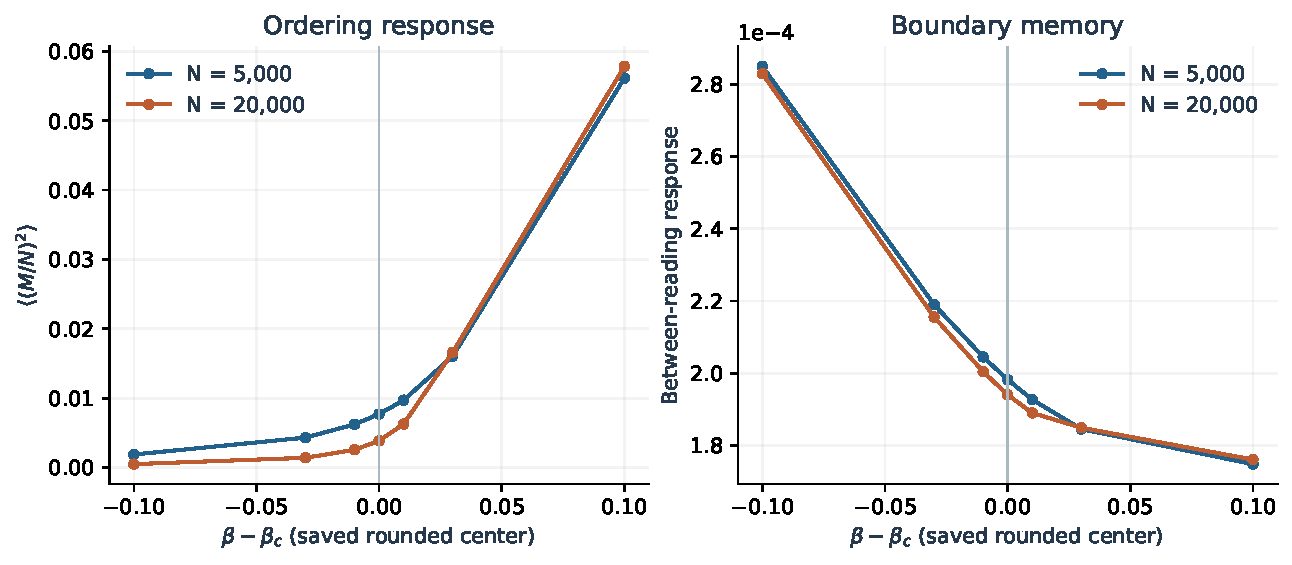
\includegraphics[width=\textwidth]{figures/transition_memory.pdf}
\caption{Recorded chain-source ordering and between-reading memory near the saved rounded critical center at $\kappa=1$. The two panels use the same finite sources and different observables. Lines connect retained data; this edition performs no thermal recalculation.\samref{SPF_FIG_TRANSITION}}
\label{fig:spin-transition}
\end{figure*}

Varying the correction-free fraction gives exact tricritical members:
\begin{table*}[tbp]\centering\small
\begin{tabular}{lccc}\toprule
Bulk components & Free fraction & $\beta_t$ & $\kappa_t$\\\midrule
Negative pairs & $1/5$ & $5/3$ & $3\log3/20$\\
Four-spin path plus four pairs & $77/461$ & $461/261$ & $261\log3/1844$\\\bottomrule
\end{tabular}
\end{table*}
Their negative sixth cumulants supply the stabilizer after the quartic term vanishes. At the displayed fixed couplings, fractions above the critical fraction have continuous first onset, and sufficiently close fractions below it have first-order onset. Critical squared magnetization scales as $N^{-1/3}$. The recorded pair control with a vanishing quartic term and a positive sixth term shows why the quartic zero alone does not classify the transition. The ratio result carries the classification: \emph{The test result suggests strong contact with the concept.}\samref{SPF_RATIO}

Negative triangles add an odd frustrated cycle as a different local component. The pure triangle/free family has an ordinary continuous first transition for every allowed free fraction and $\kappa\geq0$, with a positive quartic stabilizer. Mixing pairs, triangles and correction-free spins gives a different exact point:
\begin{align}
 \nu&=\frac9{20},&\tau&=\frac{343}{640},&f&=\frac9{640},\\
 \beta_c&=\frac{32}{15},&\kappa&=\frac{15\log3}{128}.
\end{align}
A 1920-spin bulk cell contains 432 pairs, 343 triangles and 27 correction-free spins. The fifteen-spin root and five-spin tail remain, so $N=20+1920r$. The quadratic, quartic and sextic pressure coefficients vanish, leaving
\begin{equation}
 \Phi_c(y)=-C_8y^8+O(y^{10}),\qquad C_8=\frac3{3584}.
\end{equation}
The source has a global all-field certificate as well as this local expansion. The leading stabilizer is eighth order; its boundary response need not be an eighth derivative.\samref{SPF_TRIANGLE}

With $\xi=C_8^{1/8}N^{1/8}y$, the normalized limiting density is
\begin{equation}
 p_u(\xi)\propto\exp(u\xi^2-\xi^8).
\end{equation}
The field scale is $N^{-1/8}$, the leading squared-magnetization and boundary-memory scale is $N^{-1/4}$, and the temperature window is $N^{-3/4}$. The finite calculation retains the root, tail, exact reference and physical Gaussian correction. In the completed first-correction panel, 85 of 90 observable comparisons improve; the five lower-size exceptions remain part of the result. The directed comparisons evaluate complete finite sources rather than treating the truncated local polynomial as a global Hamiltonian.\samref{SPF_OCTIC}

\begin{figure*}[tbp]\centering
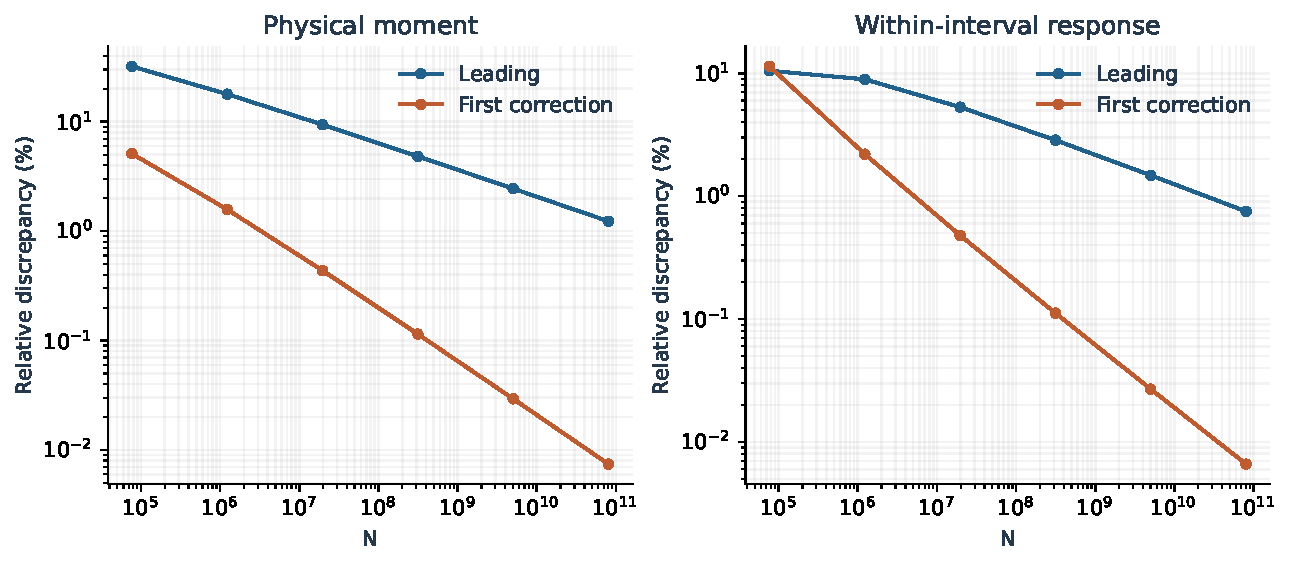
\includegraphics[width=\textwidth]{figures/octic_corrections.pdf}
\caption{Saved $u=0$ comparisons of the eighth-order leading and first-correction rules for the physical moment and within-interval response. These selected curves retain their original finite values; the complete source panel and its five lower-size exceptions have the scope stated in the text.\samref{SPF_FIG_OCTIC}}
\label{fig:spin-octic}
\end{figure*}

\subsection{A finite crossover preserves actual controls and boundary histories}

Temperature and pair/triangle fractions provide three independent physical source controls near the mixed point. In $x=\tanh^2y$, the completed control Jacobian has rank three and determinant $25/351232$. The local unfolding law is
\begin{equation}
 p(\xi)\propto\exp(\alpha\xi^2+\lambda\xi^4+\sigma\xi^6-\xi^8).
\end{equation}
The exact inverse control construction and global derivative bounds retain the associated finite source. The named dimensionless control coordinates are not the physical coupling constants of the later isotope or continuum receiver.\samref{SPF_UNFOLD}

The uniform crossover joins the eighth-order origin to merging ordered endpoints. Its simple limiting form is
\begin{equation}
 p_s(z)\propto e^{-(z^2-s)^4}.
\end{equation}
Changing variable to $t=z^2-s$ retains its half-line support and Jacobian:
\begin{equation}
 p(t)\propto\mathbf1_{t>-s}(s+t)^{-1/2}
 \exp(vt+rt^2+dt^3-g t^4),\qquad g>0.
\end{equation}
Both field endpoints and the actual rounded integer component counts enter the complete consumer. The source theorem supplies a second thermal remainder of order $N^{-3/4}$ and pressure remainder of order $N^{-7/4}$ in its stated neighborhood. All 126 first and 63 second comparison improvements pass in the selected completed crossover panel. Three reused endpoint integrals retain their earlier identities.\samref{SPF_CROSSOVER}

This thermal organization is already tied to memory. At the chain's exact $\kappa=1$ critical point, the unchanged protocol gives limiting preparation, between-reading and within-interval contributions approximately
\begin{equation}
\begin{gathered}
-0.430454602216,\\
0.000189921648477,\\
0.000344266087525.
\end{gathered}
\end{equation}
The first is a signed preparation contrast, comparing the specified state-zero start with conditional equilibrium inside its initial coarse class. The latter is not a globally stationary initial mixture. All three retain their actual middle relay, accepted state and declared heat-bath interval. Thus a bulk ordering law and a finite boundary history are measurable functions of the same source while answering different questions.\samref{SPF_TRANSITION}

\subsection{What passes to the microscopic and matter constructions}

The completed object consists of a source action, state multiplicities, ordered ports, thermal factors, finite preparation and recorded response. The exact density can answer many future weighted questions; a directed compact consumer answers a selected question using the full factor definition. The next chapters preserve that distinction when they introduce a physical generator, hidden memory and source-conditioned resolvent bounds.

For matter, this provides a constructive route from an admitted finite inventory to an interacting state. The actual Li6 phase map later in this volume retains every source constant and all contact addresses. Its conditional thermal factors carry the hidden-state normalization. The nuclear, atomic and molecular recipients then keep their actual free systems and energy payments. The underlying principle is already visible in the spin source: a complete state space can be evaluated through structured factors while its retained boundary still carries information about what happened before the next contact.

For Volume III, the same structure identifies the executable handoff. Exact integer coefficients, source-bound local factors, conditional traces, matrix intervals and retained operands are different outputs with their own useful scopes. The computation chapter of this section will connect these directly to the shared solver, native operation recipes and recorded recovery. The scientific inputs are the completed constructions developed here; this edition adds their exposition and cross-volume organization.\samref{SPF_INSTALL}

\bookchapter{Microscopic Spin Sources and the Memory of an Accepted History}
\label{ch:spin-microscopic}

\subsection{An interacting interior behind a finite boundary}

The frustrated-spin program gives Volume II a complete example of how a
small matter-facing boundary can retain a large, active interior. Pairwise
microscopic interactions generate collective boundary terms. Exact thermal
elimination determines the boundary equilibrium, while the microscopic
generator determines what happens between observations. Those operations
meet in one source without becoming the same operation. The completed work
then carries the actual interior through accepted readings, constructs
reusable response maps, and encloses very long histories with their
survival probability and complete fast remainder.

The exposition here is a Codex synthesis of the completed source
derivations. Sean Brady is originator and conceptual director; OpenAI
ChatGPT and Codex are AI research collaborators and co-authors. The
compiler, conditional-memory certificates and source-bound consumers are
identified as Codex mathematical and technical contributions in their
original records. This chapter develops that original microscopic line.
The nuclear chapters that follow apply spin representations and memory
methods to their own actual isotope sources.

\subsection{Exact thermal elimination and programmable interactions}

Take four boundary signs \(s=(s_1,s_2,s_3,s_4)\) and a hidden sign \(h\).
A full-port star of coupling \(J\) and sign row \(p=(1,p_2,p_3,p_4)\) has
energy \(-Jh(p\cdot s)\). Summing the hidden sign gives
\[
 z_{J,p}(s)=2\cosh[\beta J(p\cdot s)].
\]
For independent copies with nonnegative integer multiplicities \(w_p\),
the conditional partition functions multiply and their free energies add:
\[
 Z_s=\prod_pz_{J,p}(s)^{w_p},\qquad
 F(s)=-\beta^{-1}\log Z_s.
\]
The constant part of \(F\) remains part of absolute free energy, although
it cancels from normalized boundary probabilities.
\samref{SPM01}\samref{SPM02}

Expand in boundary characters \(\chi_A(s)=\prod_{i\in A}s_i\). A single
zero-field star has one constant, six pair terms and a quartet. Its
nonconstant scalar coefficients are
\[
\begin{gathered}
p_J=-\frac{\log\cosh(4\beta J)}{8\beta},\\
q_J=\frac{4\log\cosh(2\beta J)-\log\cosh(4\beta J)}{8\beta}.
\end{gathered}
\]
Sign copies multiply each coefficient by
\(T_A=\sum_pw_p\chi_A(p)\). This gives a finite interaction compiler:
choose the surviving character transforms, invert them to nonnegative
copy counts, and retain the resulting microscopic source.

The completed selective compiler establishes why subgroup projection
alone has a particular support. Averaging over a sign subgroup retains
its annihilator, which is closed under character multiplication.
Retaining \(s_1s_2\) and \(s_3s_4\) therefore also permits their quartet;
retaining \(s_1s_2\) and \(s_1s_3\) permits \(s_2s_3\).
Unequal nonnegative copies can remove those companion terms. Within
the fixed eight full-port unit-star dictionary, the exact minimum counts
for a pure quartet, two disjoint pairs, two overlapping pairs, and two
disjoint pairs plus their quartet are respectively \(4,8,8,2\).
Local two-port modules give the two-pair supports with two hidden spins.
These constructions compare declared supports and preserve their actual
coefficient relations.\samref{SPM02}

The integer compiler makes its count statement explicit. For a primitive
integer target transform vector \(v_A\), put
\[
 d_p=\sum_Av_A\chi_A(p),\qquad
 k_0=\frac8{\gcd(8,\{d_p-d_{p_0}\}_p)}.
\]
Fourier inversion and nonnegativity give
\[
 w_p=\frac{k_0(d_p-\min_qd_q)}8,\qquad
 N_{\min}=-k_0\min_pd_p.
\]
This is the minimum within that dictionary and transform-ratio problem.
Adding one copy of every sign pattern is an invisible uniform layer:
it changes the interior free energy while leaving normalized boundary
probabilities unchanged. The completed hidden-boundary work also gives
connected, nonisomorphic interiors with the same uniform boundary state
at every temperature, and explicit hidden interventions that distinguish
them. A complete normalized boundary equilibrium therefore need not
identify its interior source.\samref{SPM01}\samref{SPM03}

\subsection{The all-temperature ratio-one source}

Different-order coefficients in one coupling layer retain different
temperature dependence. The two-scale construction supplies the exact
identity
\[
 q_{2J}=p_{2J}-4p_J.
\]
Its ratio-one source uses pair/quartet transform units \((4,0)\) at \(J\)
and \((-1,-1)\) at \(2J\). The resulting coefficients satisfy
\[
 P=4(4p_J-p_{2J})=-4q_{2J}=Q<0,
\]
so the complete boundary free energy is
\[
 F(s)=C(\beta)+P(\beta)s_1s_2(1+s_3s_4).
\]
One parity sector of the second pair disables the first pair's effective
interaction; the other doubles it. The ratio \(Q/P=1\) holds for every
\(\beta,J>0\), while the strengths themselves vary with beta.
The derivation follows directly from the two log-cosh functions; the
positivity of \(q_{2J}\) keeps the denominator nonzero.
\samref{SPM04}\samref{SPM05}

The sixteen weak and eight strong copies total 24 hidden spins. More
generally, transform units \((4d,-d,0,-n)\) give quartic/pair ratio \(n/d\)
with \(20d+4|n|\) hidden copies. The completed native reconstruction
evaluated ratios \(1,2,1/2,-1,3/2\), requiring \(24,28,44,24,52\) copies.
Exact character cancellation and the log-vector identity establish the
all-temperature statement; nine beta samples check the constructed
sources. The prior one-scale 32-copy ratio was \(1.004288551457\) at
beta one, with derivative \(0.658276967618\). The two-scale source
has ratio one and derivative zero throughout. For this exact thermal
ratio construction, \emph{The test result suggests strong contact with
the concept.}\samref{SPM04}

The original microscopic memory model is this ratio-one source at \(J=1\).
Its actual groups, rather than a new effective surrogate, are retained in
the source artifact:
\[
\begin{array}{c|c|c}
\text{sign pattern }a_g&J_g&m_g\\
\hline
(1,1,-1,-1)&1&4\\
(1,1,-1,1)&1&4\\
(1,1,1,-1)&1&4\\
(1,1,1,1)&1&4\\
(1,-1,-1,-1)&2&2\\
(1,-1,-1,1)&2&1\\
(1,-1,1,-1)&2&1\\
(1,-1,1,1)&2&2\\
(1,1,-1,1)&2&1\\
(1,1,1,-1)&2&1
\end{array}
\]
This 24-hidden source differs from the later eight-hidden parity module
used to realize an isotope quartet's ground energy. Here the full
conditional partition function and the actual kinetics of both coupling
layers travel together.\samref{SPM06}

\subsection{Twenty-eight spins, exact multiplicities and the original clock}

If \(c_g\) is the number of plus signs in group \(g\), the exact energy
and multiplicity are
\[
 E(s,c)=-\sum_gJ_g(a_g\cdot s)(2c_g-m_g),\qquad
 \mu(c)=\prod_g{m_g\choose c_g}.
\]
There are \(16\prod_g(m_g+1)=1{,}440{,}000\) grouped coordinates,
representing all \(2^{28}=268{,}435{,}456\) microscopic configurations.
The count grouping retains the binomial number of labelled configurations
in every class. Rates into another count class depend only on the
present class, including the number of available microscopic flips.
The resulting reduction is exact for these boundary consumers and
retains unequilibrated count preparations.\samref{SPM07}

For finite beta and couplings, every Gibbs weight is positive. Write
\[
\begin{gathered}
Z_s=\prod_g[2\cosh(\beta J_ga_g\cdot s)]^{m_g},\\
\nu_s=\frac{Z_s}{\sum_bZ_b},\\
\chi_s(c)=\frac{\mu(c)e^{-\beta E(s,c)}}{Z_s},\\
\pi_{s,c}=\nu_s\chi_s(c).
\end{gathered}
\]
These are normalized boundary, conditional and joint laws. Conditional
elimination preserves the interior thermodynamics through \(Z_s\);
microscopic evolution uses the complete state \((s,c)\).

The original clock assigns attempt rate one to each boundary spin and
positive fixed rate \(\gamma_g\) to each hidden spin in group \(g\).
With \(F_i(c)=\sum_gJ_ga_{gi}(2c_g-m_g)\), boundary and hidden rates are
\[
 \rho_i(s,c)=\frac1{1+e^{2\beta s_iF_i(c)}},\qquad
 h_g(s)=\frac1{1+e^{-2\beta J_ga_g\cdot s}},
\]
\[
\begin{gathered}
c_g\longrightarrow c_g+1:
      (m_g-c_g)\gamma_gh_g(s),\\
c_g\longrightarrow c_g-1:
      c_g\gamma_g[1-h_g(s)].
\end{gathered}
\]
The binomial identity
\({m\choose c}(m-c)={m\choose c+1}(c+1)\) establishes hidden detailed
balance; the boundary heatbath ratio gives its corresponding Gibbs
balance. The resulting column generator \(L\) is reversible for \(\pi\).
The executed memory source uses beta one and common \(\gamma=1\);
time remains measured on this attempted-spin clock.\samref{SPM08}

\subsection{Exact projection retains the initial hidden forcing}

Let \(C\) sum hidden counts, \(R\) lift a boundary distribution by the
actual conditional law \(\chi_s\), and \(CR=I\). Decompose
\[
\begin{gathered}
p=Rq+r,\\
q=Cp,\\
Cr=0,\\
A=CLR,\\
G=(I-RC)LR,\\
D=(I-RC)L\big|_{\ker C}.
\end{gathered}
\]
Solving the residual equation gives the exact boundary evolution
\[
 q'(t)=Aq(t)+g(t)+\int_0^tK(t-u)q(u)\,du,
\]
\[
 g(t)=CLe^{tD}r_0,\qquad K(t)=CLe^{tD}G.
\]
Both terms are source operands. \(A\) is the conditionally averaged
microscopic generator. A heatbath built only from the integrated
boundary free energy is a different generator, whose equal equilibrium
does not assign these microscopic rates.\samref{SPM07}\samref{SPM09}

Global reversal \((s,c)\mapsto(-s,m-c)\) preserves energy, multiplicity
and rates. Its two sectors have 720,000 coordinates each. For representative
and partner probabilities, \(x=p_{\rm rep}+p_{\rm partner}\) and
\(y=p_{\rm rep}-p_{\rm partner}\) evolve independently under \(L_+\)
and \(L_-\). A boundary mask with values \(m_b,m_{\bar b}\) acts by
\[
 x_{\rm new}=\tfrac12[(m_b+m_{\bar b})x+(m_b-m_{\bar b})y],
\]
with the corresponding expression for \(y_{\rm new}\).
Reversal-invariant pair selections have \(m_b=m_{\bar b}\); every finite
history of those masks and unchanged-source propagation is determined
by the plus sector for arbitrary actual initial preparations.
Orientation-sensitive selection needs both sectors. This reduction
retains the hidden residual instead of equilibrating it.
\samref{SPM07}

The completed eight-column plus kernel covers seventeen lags through
\(t=0.02\). Its shared-lag values agree with the earlier full-source
kernel within \(6.94\times10^{-17}\). For the actual hidden-point
preparation, omitting \(g\) produces endpoint error \(0.0180851\);
retaining it gives fine-grid error \(9.029\times10^{-8}\).
For the actual accepted two-readout substate the corresponding errors
are \(1.655\times10^{-5}\) and \(4.493\times10^{-10}\).
The accepted state remains unnormalized: its mass is the probability of
the preceding history. Its residual forcing survives the intervention.
\samref{SPM09}

The sampled Volterra solver exhibits the expected fourfold error
reduction when its grid spacing halves. A retained tiny negative
coordinate records that solver's numerical positivity behavior;
direct microscopic uniformization supplies the positive propagation
baseline. The source symmetry identities are exact, the large-source
propagation is qualified float64, and the numerical integration and
series-truncation accounts retain their separate recorded scopes.
For the complete reduced kernel and retained-memory reconstruction,
\emph{The test result suggests strong contact with the concept.}
\samref{SPM09}

\subsection{A small covariance controls the entire hidden complement}

Reversibility supplies a stronger uniform result. In Gibbs-weighted
coordinates let \(H=-\Pi^{-1/2}L\Pi^{1/2}\), let \(\mathcal J\) be the
conditional isometry, and let \(Q=I-\mathcal J\mathcal J^T\). Define
\[
\begin{gathered}
a=\mathcal J^TH\mathcal J,\\
b=QH\mathcal J,\\
d=QHQ\big|_{\operatorname{ran}Q},\\
{\cal V}=b^Tb,\\
{\cal K}(t)=b^Te^{-td}b.
\end{gathered}
\]
At fixed boundary, hidden heatbath conditional expectations commute on
the independent product law. A product of centered single-spin functions
has eigenvalue equal to the sum of its participating attempt rates.
Every nonconstant hidden direction therefore costs at least
\(\gamma_*=\min_g\gamma_g>0\). Boundary heatbaths contribute a positive
operator bounded by \(4I\). Consequently
\[
 \gamma_*I\preceq d\preceq
 \left(4+\sum_gm_g\gamma_g\right)I.
\]
For common \(\gamma\), write \(\Lambda=4+24\gamma\). The complete kernel
and its Laplace transform obey
\[
\begin{gathered}
e^{-\Lambda t}{\cal V}\preceq{\cal K}(t)
       \preceq e^{-\gamma t}{\cal V},\\
\frac{\cal V}{z+\Lambda}\preceq\widehat{\cal K}(z)
       \preceq\frac{\cal V}{z+\gamma},\\
z>0.
\end{gathered}
\]
The hypotheses are a finite independent-star source, finite positive
Gibbs weights, fixed positive hidden rates and the specified microscopic
clock. They include every hidden-copy count.\samref{SPM08}

The coefficient \({\cal V}\) is computed from the four-by-four
conditional covariance of the actual boundary flip rates. It includes
every covariance cross term. It is independent of hidden attempt speed
at fixed source and boundary clock. Since
\(0\preceq H_B\preceq4I\),
\[
 0\preceq{\cal V}\preceq4a-a^2\preceq4I,\qquad
 \int_0^\infty{\cal K}(t)\,dt=b^Td^{-1}b\preceq a.
\]
The latter follows by completing the full positive quadratic form.
The exact response is the Schur inverse
\([zI+a-\widehat{\cal K}(z)]^{-1}\), with its reciprocal boundary
background retained. An eight-coordinate coefficient controls output
coupling to all 719,992 residual directions per sector.
\samref{SPM08}

For the actual beta-one source, directed calculations give even/odd
ranks \(7,8\) and norm uppers \(0.11541111,0.11540590\), about 35 times
tighter than the universal four. The even stationary direction supplies
its one-dimensional kernel. At \(T=0.2\), the saved complete-boundary
total-variation errors for \(\gamma=1/4,1,4,16\) are
\(0.000830225,0.000715785,0.000456950,0.000181530\).
Their uniform uppers are
\(0.0439544,\allowbreak0.0418539,\allowbreak0.0348203,\allowbreak0.0195585\).
All sixteen saved time/speed responses satisfy their complete-source
budgets. The comparison varies the actual hidden response speed while
retaining the same source and boundary attempts. Its exact reference
is \(A=CLR\); both reversal sectors are included for the full boundary
distribution. These new small-matrix results reused the finished source
trajectories.
\emph{The test result suggests strong contact with the concept.}
\samref{SPM10}

\subsection{Preparation, between-reading and within-wait payments}

For total waiting time \(T\), define
\[
 \psi(T)=\frac{1-e^{-\gamma T}}\gamma,\qquad
 \Phi(T)=\frac{\gamma T-1+e^{-\gamma T}}{\gamma^2},
 \qquad\bar v\geq\|{\cal V}\|.
\]
Any finite ordered history of boundary contractions retains the actual
initial \(r_0\). The sharper complete-history bound is
\[
 \|q_{\rm actual}-q_{\rm coarse}\|_{\nu^{-1}}
 \leq\sqrt{\bar v}\psi(T)\|r_0\|_{\pi^{-1}}
      +\bar v\Phi(T)\|q_0\|_{\nu^{-1}}.
\]
Its three signed responses have payments
\[
\begin{split}
 E_{\rm preparation}&\leq\sqrt{\bar v}\psi(T)\|r_0\|,\\
 E_{\rm between}&\leq\bar v
       [\Phi(T)-\sum_i\Phi(t_i)]\|q_0\|,\\
 E_{\rm within}&\leq\bar v\sum_i\Phi(t_i)\|q_0\|.
\end{split}
\]
The source norms in the first display specify those in the second.
The identity \(\Phi(s+t)-\Phi(s)-\Phi(t)=\psi(s)\psi(t)\)
pays the hidden relay between waits. Masks contract both boundary and
residual norms, so the budget needs no additional factor counting
readings. Conditioning divides by the actual acceptance mass.
\samref{SPM11}

For two waits of \(0.01\), each accepting \(s_0s_1=1\), conditional
boundary-one preparation has weighted error \(0.000245118417\),
below payment \(0.000628042124\). Actual acceptance is
\(0.999921864086\), versus coarse-reference \(0.999921316288\).
The hidden-point preparation has weighted residual norm \(36423.4512\)
and initial forcing \(L^1\)-norm \(1.90907536\); the accepted
post-readout state has \(0.111436857\) and \(0.00172853354\).
These are their actual preparation costs. Their retained signed
responses can be much smaller than a general norm budget, and remain
available without removing that budget.\samref{SPM10}

\subsection{Cache the complete consumer and continue its hidden columns}

The measured fixed-endpoint task selected direct response reuse:
eight columns of \(Ce^{TL}R\) took \(5.93\) seconds to construct,
compared with \(77.88\) seconds for seventeen kernel lags. The kernel
resolves memory; the endpoint cache answers its own specified output.
For repeated readings the reusable object is the complete ordered
consumer
\[
 {\cal H}_{\rm protocol}
       =CM e^{L/100}M e^{L/100}R.
\]
Separate projected wait maps insert a conditional reset between them.
The complete cache instead retains the full hidden columns after each
reading. Two actual residual columns supplement its eight conditional
inputs, giving \(q={\cal H}_{\rm protocol}q_0+Z\theta\) for the admitted
residual span and actual positive preparation.\samref{SPM09}\samref{SPM12}

All 44 retained preparations agree with direct microscopic histories
within \(2.22\times10^{-16}\). Their bank stores ten full columns in
43,136,071 compressed bytes. Construction takes \(12.269\) seconds;
direct propagation of 44 preparations takes \(48.080\) seconds;
installed native application takes \(0.07434\) seconds. The recorded
reuse ratio is \(646.76\), with first-cohort ratio \(3.895\) including
construction. These are measured same-worker batches with storage
charged to the build.\samref{SPM12}

The next completed consumer advances those ten columns once:
\[
 B=T[R,r_{\rm point},r_{\rm post}],\qquad
 B_s=e^{sL}B,\qquad q_m=mCB_sx.
\]
One unmasked continuation bank serves alternative terminal readouts.
Its inherited residual has the complete small Gram
\[
 G_{\rm cut}=B^TQ^T\Pi^{-1}QB,\qquad
 \|r_{\rm cut}\|_{\pi^{-1}}^2=x^TG_{\rm cut}x.
\]
Every cross term and the accepted prefix mass remain. If a comparison
has different prefix mass, acceptance difference contains its source
mean times that mass difference plus the centered signed response.
Complementary acceptance and rejection defects have opposite signs.
\samref{SPM13}\samref{SPM14}

All 44 three-wait histories match within \(5.56\times10^{-16}\).
For the actual post-readout preparation, two further accepted readings
raise residual norm from \(0.1114368572\) to \(0.2136700067\).
For the hidden point, overlapping pair12 exposes a memory acceptance
change \(-0.004252509014\), versus \(+3.82127050\times10^{-5}\) for
pair01: \(111.285\) times the magnitude with opposite sign. A fresh
parity query uses the retained bank with zero microscopic propagation.
This is actual source memory reused by a newly chosen consumer.
\samref{SPM13}

\subsection{The accepted-return mode retains its own interior}

For the proper nonempty pair mask \(M\) and wait \(s=1/100\), repeated
accepted returns use
\[
 K_{\rm ret}=Me^{sL}M
\]
on the 360,000-coordinate accepted even sector. Its symmetric weighted
counterpart is \(\mathcal K_{\rm ret}=Me^{-sH}M\). Finite positive source
rates make the source irreducible; its positive-time transition matrix
is strictly positive. Reversible weighting makes the accepted principal
block positive definite. Its largest eigenvalue is therefore simple,
strictly between zero and one, with a positive mode. Normalized positive
accepted inputs converge to that mode's actual preparation. The
acceptance ratio tends to \(\lambda_1\), and the survival rate on the
original clock is \(-\log\lambda_1/s\). The limiting hidden residual is
part of this state.\samref{SPM14}

The completed source calculation encloses
\[
 \lambda_1\in
 [0.9999999103303717,\ 0.9999999103304213],
\]
\[
 -\log\lambda_1/s\in
 [8.96695828353,\ 8.96696322351]\times10^{-6}.
\]
The survival e-fold lies between \(11{,}152{,}047.5223\) and
\(11{,}152{,}053.6662\) readings. Actual hidden residual norm is
approximately \(0.00076429382521336\). At the same cut, conditional
reset gives acceptance \(0.9999998972146613\); retaining the interior
reduces per-reading loss by approximately \(12.76\) percent.
These are properties of the actual limiting mode and its declared
readout, with finite-input amplitudes still required for finite survival.
\samref{SPM15}

The hidden gap also pays the entire remaining space. In symmetric
coordinates put \({\cal G}=(I-\mathcal K_{\rm ret})/s\). Since \(\|H\|\leq56\),
\[
\begin{gathered}
{\cal G}\succeq \eta_0MHM,\\
\eta_0=\frac{1-e^{-0.56}}{0.56}=0.7656981002699734\ldots,
 \\
d_5({\cal G})\geq \eta_0.
\end{gathered}
\]
Only four directions can have defects below that threshold. The four
computed defects are approximately
\(8.96696035\times10^{-6},8.59490215\times10^{-5},
0.03684778302,0.03685638161\). Exact thin contractions and directed
small-matrix certificates retain source-table, stencil, normalization
and residual payments. For the actual return-mode result,
\emph{The test result suggests strong contact with the concept.}
\samref{SPM15}\samref{SPM18}

\subsection{Four slow modes with the full fast remainder}

The complete finite-history consumer retains all four slow modes as a
block. For exact orthonormal stored subspace \(W\), small compression
\(T=W^T{\cal G}W\) and residual \(F={\cal G}W-WT\), separation from
\(\eta_0\) gives
\[
 \delta=\frac{\|F\|}{\eta_0-\operatorname{top}T}
          \leq7.06531\times10^{-12}.
\]
Writing the exact slow basis as \(Z=WD+(I-WW^T)Z\), \(D=W^TZ\),
yields the quadratic
block payment
\[
\begin{gathered}
\|Z^T{\cal G}Z-T\|
 \leq2b\|T\|+2\|F\|\delta+g_{\max}\delta^2,\\
b=1-\sqrt{1-\delta^2}.
\end{gathered}
\]
Here \(g_{\max}=(1-e^{-0.56})/s\) bounds the complete defect operator.
It is at most \(2.21507\times10^{-21}\); the full small-block error,
including retained source/Ritz arithmetic, is at most
\(2.469987\times10^{-12}\). Close slow pairs need no separate
eigenvector identification. The complete fast contraction is
\(\rho\leq0.992343018997301\).\samref{SPM16}\samref{SPM17}

For an actual accepted prefix \(p\), let \(y=\Pi^{-1/2}p\).
An immediate readout \(f\) has weighted terminal vector
\(a_f=M\Pi^{1/2}f\), and its response is
\(u_f(m)=a_f^T\mathcal K_{\rm ret}^my\). The mass readout gives
\(M_m\), and conditional response is \(u_f(m)/M_m\).
Let \(V\) be the actual stored mode columns, \(T_0\) their retained
small Ritz matrix, \(y_0\) a stored weighted input, and
\(\epsilon_B\) the complete small-block payment above. Put
\(v\geq\|V\|\), \(Y\geq\|y_0\|\), \(e\geq\|Z-V\|\),
\(c_0\geq\|V^Ty_0\|\), \(c_Z=c_0+eY\), and
\(r_0^{\rm fast}\geq\|(I-WW^T)y_0\|\).
Choose \(\lambda_*<1\) bounding the exact slow return and retained small
power. The complete state-response inequality, valid for every integer
\(m\geq0\), bounds
\(\|\mathcal K_{\rm ret}^my_0-V(I-sT_0)^mV^Ty_0\|\leq E_m\), where
\[
\begin{split}
 E_m={}&e\lambda_*^m(c_Z+vY)
       +vms\epsilon_B\lambda_*^{m-1}c_Z\\
       &+\rho^m(r_0^{\rm fast}+\delta Y).
\end{split}
\]
The middle term is zero at \(m=0\). The first term pays the stored
subspace and Gram normalization, the second telescopes the small
power error, and the third retains the entire fast complement.
For a stored terminal vector \(a_0\), with physical input/readout
errors \(\sigma_y,\sigma_a\), the actual scalar-response error is bounded by
\[
 \|a_0\|E_m+\sigma_a\lambda_*^mY
       +(\|a_0\|+\sigma_a)\lambda_*^m\sigma_y.
\]
The implementation additionally includes directed small-product
arithmetic and both coefficient-contraction errors. Prefix
reconstruction enters \(\sigma_y\) with the actual source
normalization and its earlier accepted mass. An immediate readout and
a readout after an unmasked wait have their own terminal vectors;
the latter carries its complete source-propagation payment.
For numerator and mass errors \(E_u,E_M\),
\[
 \left|\frac{u}{M}-\frac{\widehat u}{\widehat M}\right|
 \leq
 \frac{E_u+|\widehat u/\widehat M|E_M}{\widehat M-E_M},
 \qquad\widehat M>E_M.
\]
The survival denominator remains inside the prediction.
\samref{SPM17}

The retained numerical source scopes are part of this construction.
The large microscopic stencil and stored history columns use the
qualified floating propagation from their original campaigns. Exact
binary-rational thin contractions and native directed products certify
the stored operands they receive. The return-mode and four-mode
certificates then pay the identified source-table, action, normalization,
residual and small-block errors needed for their stated enclosures.
Thus the small consumer has an explicit route back to the original
state and readout, retaining the spin Hamiltonian, the physical
preparation and its nonzero fast component.\samref{SPM15}\samref{SPM17}\samref{SPM19}

The completed panel has 44 preparations, seventeen readout/mass rows,
and twenty checkpoints through \(10^9\) additional accepted readings.
All 44 have positive enclosed denominators from 2048 onward on that
panel. The widest conditional interval is \(5.551\times10^{-7}\) at
4096 readings and \(0.001798\) at \(10^9\); the later width includes
the accumulated retained Ritz payment. At \(10^9\), equilibrium-zero,
hidden-point and post-readout inputs retain surviving masses
\(1.1404748,1.0599825,1.0297777\), each times \(10^{-39}\).
All 306 full-sector outcome/mass comparisons and eighteen independent
spectral/block identities pass. The consumer reuses completed modes;
it performs no new eigeniteration. \emph{The test result suggests
strong contact with the concept.}\samref{SPM16}

This line supplies a concrete matter-construction method: form the
complete interior source, derive the visible recipient, and retain
the preparation and complement that carry its next response.
Its action, normalization and chronological payments connect to the
Volume I record and preparation account. Its source-bound caches,
native thin contractions and recoverable consumers connect to
Volume III computation. The completed four-mode result leaves a
focused numerical successor: sharpen the directed small Ritz
arithmetic on the same source to improve very long conditional
intervals. The full source, original clock and paid complement
already belong to the achieved construction.

\bookchapter{Composition, thermal cancellation and intrinsic spin memory}
\label{ch:spin-composition}

\subsection{Which changes alter a response, and which change only its clock?}

A spin source can keep the same visible inventory while changing the hidden preparation that supplies its next response. The completed composition sequence gives that statement a detailed mechanism. Exact component factors turn a change in graph composition into a covariance under the full thermal field. A particular integer change cancels its first field term. A unique moment condition removes the next term, and two derived temperature corrections suppress the complete count response further. At sixth order a new hidden interaction survives every shared thermal correction. Its rational dependence on relaxation scale identifies the hidden directions that a receiver detects.\samref{SPC01}\samref{SPC02}\samref{SPC05}

The sequence uses the Kac-normalized pair/triangle/free-spin family introduced in Chapter~\ref{ch:spin-foundation}, its literal fifteen-spin root and the original reading interval $\theta=1/3$. A complementary kinetic calculation uses a distinct four-boundary/24-hidden-spin source. There the microscopic boundary flip keeps the actual hidden coordinates; replacing it by a thermal-boundary flip changes individual edge rates. The completed comparison determines exactly when that change could be a common clock multiplier, and finds that the retained source does not satisfy the condition. These two constructions meet at the source-to-receiver interface while retaining their different Hamiltonians and clocks.\samref{SPC06}\samref{SPC07}

The Hamiltonians, component inventories, preparations and readouts are model assignments inherited from their original sources. The covariance identities, cancellation rules, sixth-order decomposition and kinetic comparison below are completed deductions from those assignments. They are recorded as Codex contributions within Sean Brady's composition investigation. Sean Brady is the originator and conceptual director; OpenAI ChatGPT and Codex are AI research collaborators and co-authors. The completed source campaigns classify their results as: \emph{The test result suggests strong contact with the concept.}\samref{SPC10}\samref{SPC11}\samref{SPC12}\samref{SPC13}\samref{SPC07}

\subsection{An exact component law on a fixed spin inventory}

The composition Hamiltonian and coupling are
\begin{equation}
 H=-\frac{M^2-N}{2N}+\kappa C,\qquad
 \kappa=\frac{15\log3}{128}.
\end{equation}
Here $M$ is total spin, $C$ is the retained component interaction account, and the root plus its fixed pair and three free spins occupy twenty sites. For the remaining $n=N-20$ sites, the integer pair, triangle and free counts satisfy
\begin{equation}
 2P+3T+F=n.
\end{equation}
At fixed $N,\beta,\kappa$ and fixed source center, let $X=\tanh^2y$ and define
\begin{equation}
 b=\tanh(2\beta\kappa),\qquad a=\frac{3b}{1+b+b^2}.
\end{equation}
The exact normalized pair and triangle traces are
\begin{align}
 \frac{Z_{\rm pair}(y)}{Z_{\rm pair}(0)}
 &=\cosh^2y(1-bX),\\
 \frac{Z_{\rm triangle}(y)}{Z_{\rm triangle}(0)}
 &=\cosh^3y(1-aX).
\end{align}
Thus composition changes a complete positive field law through two known logarithmic factors, rather than an assumed phenomenological memory coefficient.\samref{SPC01}

For literal boundary value $j$, let $R_j(y)$ be its positive fifteen-spin root row, reconstructed from the original integer multiplicities. Up to boundary-independent factors, the full Gaussian weight is
\begin{equation}
\begin{aligned}
 W_j(P,T)={}&\int_0^\infty R_j(y)e^{-Ny^2/(2\beta)}\\
 &\cosh^{N-15}y(1-bX)^{P+1}(1-aX)^T\,dy.
\end{aligned}
\end{equation}
The extra pair is the fixed pair outside the fifteen-spin root. The full source retains its absolute pressure constants. Their common score cancels from normalized preparation and response derivatives, while their source values remain recorded. The origin and infinite upper tail belong to the field law.\samref{SPC01}

Write $R_\Sigma=\sum_jR_j$, $r_j(y)=R_j/R_\Sigma$, and let $\mu$ be the normalized complete field law with root $R_\Sigma$. The boundary probabilities are $\pi_j=\mathbb E_\mu r_j$. Differentiating the actual component factors gives
\begin{align}
 \partial_P\pi_j&=\operatorname{Cov}_\mu(r_j,\ell_P),
 &\ell_P&=\log(1-bX),\\
 \partial_T\pi_j&=\operatorname{Cov}_\mu(r_j,\ell_T),
 &\ell_T&=\log(1-aX).
\end{align}
These are exact finite-source identities. Continuous count variables provide analytic comparisons between positive partition functions; actual graph endpoints retain integer counts. A derivative is not assigned to a fractional graph.\samref{SPC01}

The covariance also supplies a quantitative payment. If $K_j$ bounds $|dr_j/dX|$, put $\mathcal A=\max_jK_j/\pi_j$ and $\mathcal L_P=b/(1-b)$, $\mathcal L_T=a/(1-a)$. The independent-copy covariance identity yields
\begin{equation}
 \operatorname{osc}_j(\partial_i\log\pi_j)
 \leq2\mathcal A\mathcal L_i\operatorname{Var}_\mu(X).
\end{equation}
The root polynomials give explicit finite $K_j$ and a positive probability bound. Propagating this score through the complete receiver pays the between-reading derivative by $12\mathcal A\mathcal L_i\operatorname{Var}(X)$ and the within-interval derivative by $8\mathcal A\mathcal L_i\operatorname{Var}(X)$. The whole field supplies the variance; every preparation and dynamical endpoint remains in the receiving functional.\samref{SPC01}\samref{SPC08}

\subsection{The complete receiver and the compensated direction}

The receiver is the original three-reading protocol. On its retained quotient let $E_\pm=e^{\theta Q_\pm}$, $\mathsf H=(E_++E_-)/2$, and let $p$ be the normalized accepted preparation. Define
\begin{align}
 q&=\mathbf1^t\mathsf H p,
 &r&=\mathbb E_p\rho,
 &a_\theta&=\frac{1+e^{-2\theta r}}2,\\
 F_B&=\mathbf1^t\mathsf H^3p-q^3,
 &F_W&=q^3-a_\theta^3.
\end{align}
The literal flip rate is $\rho_b=w_{b\mathbin{\mathrm{xor}}1}/(w_b+w_{b\mathbin{\mathrm{xor}}1})$. Complete differentiation changes $p$, $r$, each propagator and every relay term. In particular, the middle $E_+$ derivative in the ordered relay remains present. For a score oscillation $G$, the original $\theta=1/3$ gives the bounds $|\partial F_B|\leq6G$ and $|\partial F_W|\leq4G$.\samref{SPC08}

The hidden feedback has the full reversible form
\begin{equation}
 \Gamma(z)=f^t(zI+D)^{-1}f,\qquad
 f_b=2(\rho_b-r)\sqrt{p_b},\qquad z>0,
\end{equation}
with the preparation direction projected out of $D$. Both its forcing and its operator change under a source derivative:
\begin{equation}
 \partial\Gamma
 =2(\partial f)^t(zI+D)^{-1}f
 -f^t(zI+D)^{-1}(\partial D)(zI+D)^{-1}f.
\end{equation}
The resulting score bound is $(5/z+6/z^2)G$. These formulas explain why cancellation of a complete response is stronger than cancellation in one weight, one rate or one forcing vector.\samref{SPC08}

The two memory channels have complementary operational meanings. The between-reading quantity compares the actual ordered three-reading return with the product formed from its one-interval return. The within-interval quantity compares that one-interval return product with the constant-rate expression using the actual source mean. The two differences retain their signs. Neither is replaced by the variance of a rate distribution. Their composition derivatives can vanish at a selected order even when the underlying memory observables remain nonzero. In the feedback derivative, the second term above is just as necessary as the forcing derivative: changing composition changes the operator that propagates hidden information as well as the information injected into it.\samref{SPC08}

The center subtraction has a similarly explicit role. Each complete thermal quantity compares the integrated source response with the source-center response at the same temperature. A count change at fixed temperature and center has zero derivative on the center side. Its complete center value remains stored, while the count susceptibility comes from the integrated source. Along a changing-temperature path the center has its own tangent. The corrected families below always evaluate the count derivative at their corrected fixed temperature, preserving that distinction between selecting a source and differentiating an observable on it.\samref{SPC08}

The inventory-preserving direction
\begin{equation}
 h=(-12\ {\rm pairs},+7\ {\rm triangles},+3\ {\rm free})
\end{equation}
has score $\ell_h=-12\log(1-bX)+7\log(1-aX)$. At the retained critical temperature $\beta_c=32/15$, the factors are $b=1/2$, $a=6/7$, and
\begin{equation}
\begin{gathered}
\ell_h'(X)=-\frac{(15/7)X}{(1-X/2)(1-6X/7)},\\
\ell_h(X)=-\frac{15}{14}X^2+O(X^3).
\end{gathered}
\end{equation}
The linear field term cancels exactly. At a nearby actual temperature the payment retains the departure:
\begin{equation}
 \operatorname{osc}(g_h)\leq
 2\mathcal A\left[
 |12b-7a|\operatorname{Var}(X)
 +\frac{c_\beta}{2}\operatorname{Cov}(X,X^2)\right],
\end{equation}
where $c_\beta=12b^2/(1-b)+7a^2/(1-a)$. Setting the critical coefficient to zero at every finite temperature would omit the first term and give the wrong signed expansion.\samref{SPC01}

\subsection{Critical scaling and a unique moment cancellation}

The endpoint family is specified by $\Phi_x=\Phi_{xx}=\Phi_{xxx}=0$, with
\begin{equation}
\begin{aligned}
 \Phi(x)={}&-\frac12\log(1-x)
 -\frac{\operatorname{atanh}^2\sqrt{x}}{2\beta}\\
 &+\frac{\nu}{2}\log(1-bx)+\frac{\tau}{3}\log(1-ax).
\end{aligned}
\end{equation}
Its critical parameters are
\begin{equation}
\begin{gathered}
(\beta_c,\nu_c,\tau_c)=
 \left(\frac{32}{15},\frac9{20},\frac{343}{640}\right),\\
C_8=\frac3{3584},\\
\delta=(NC_8)^{-1/4}.
\end{gathered}
\end{equation}
The coefficient Jacobian has determinant $25/351232$, so the three endpoint controls define an analytic branch through this point. Put $x_0=s\delta$. Bounded $O(N^{1/4})$ composition offsets and rounded counts lead to the complete limiting law
\begin{equation}
 d\mu_{s,v}(U)=Z^{-1}U^{-1/2}
 e^{-(U-s)^4+v(U-s)}\,dU,\qquad U>0.
\end{equation}
The square-root origin factor is retained. Global quartic domination and the original Gaussian tail control the entire field, giving generic $O(N^{-1/2})$ and compensated $O(N^{-3/4})$ count susceptibilities on compact positive $s$ families.\samref{SPC14}

Let $V=\operatorname{Var}(U)$, $C_3=\operatorname{Cov}(U,U^2)$, and $\mathcal B=81\log3/112$. For each complete response $F_i$,
\begin{align}
 \partial_PF_i&=-\frac V2L_i\delta^2+O(\delta^3),\\
 \partial_TF_i&=-\frac{6V}{7}L_i\delta^2+O(\delta^3),\\
 \partial_hF_i&=\mathcal Q(s,v)L_i\delta^3+O(\delta^4),\\
 \mathcal Q(s,v)&=\mathcal B sV-\frac{15}{14}C_3.
\end{align}
The $L_i$ are complete critical root/clock tangents. Their shared field coefficient includes the actual temperature slope $\beta_*'(0)=3/5$ as well as the compensated quadratic score. The between and within tangents are approximately $-0.01337089297098$ and $-0.02125803744488$.\samref{SPC02}

Cancellation requires a unique tilt, rather than a chosen response fit. Give independent $U,U'$ the pair law weighted by $(U-U')^2$, normalized by $2V$. Then
\begin{equation}
 \frac{C_3}{V}=\mathbb E_{\rm pair}(U+U'),\qquad
 \partial_v(C_3/V)=\operatorname{Var}_{\rm pair}(U+U')>0.
\end{equation}
Its tilted mean ranges from zero to infinity. Hence every $s>0$ has exactly one $v_*(s)$ satisfying
\begin{equation}
 \frac{C_3}{V}=\frac{27\log3}{40}s.
\end{equation}
The retained roots are approximately
\[
\begin{array}{c|r}
s&v_*(s)\\\hline
1/2&-8.103016840846506\\
2&-8.788848955616438\\
4&-64.23014856254630
\end{array}
\]
The signed coefficient $\mathcal Q$ is positive below this tilt and negative above it.\samref{SPC03}

Actual sources use nearest integers
\begin{equation}
\begin{gathered}
P=\operatorname{nint}\!\left(\frac{n\nu_*(x_0)}2-\frac{2v_*}{\delta}\right),
 \\
T=\operatorname{nint}\!\left(\frac{n\tau_*(x_0)}3\right),
 \\
F=n-2P-3T.
\end{gathered}
\end{equation}
Their two rounding errors $e_P,e_T$ remain within $[-1/2,1/2]$ and enter every later coefficient. The derivative $\partial_h$ always holds the actual temperature, center and $N$ fixed. It is not differentiation along the temperature-adjusted family.\samref{SPC03}

The limiting free-spin fraction is $9/640$, so the bounded offset and rounding rules leave all three component populations nonnegative beyond a common size threshold. The uniform statements quantify the entire admitted family, rather than only the finite sizes evaluated. Their temperature accuracy is explicit: the signed leading law uses an $O(N^{-1})$ approximation to the endpoint branch, with progressively sharper correction errors at later orders. Integrating the exact derivative over a fixed-temperature count segment also distinguishes susceptibility from an endpoint difference. A segment of length $O(N^{1/4})$ has the corresponding generic $O(N^{-1/4})$ and compensated $O(N^{-1/2})$ upper estimates when it stays in the admitted family.\samref{SPC02}\samref{SPC03}

\subsection{Two shared corrections and their exact symmetry mechanism}

Write $\mathfrak f(U)=\mathcal B sU-(15/14)U^2$ and
$T_2=\operatorname{Cov}(\mathfrak f,U^2)=\mathcal Q_v<0$ at $v_*$. At the first moment cancellation, the full fourth coefficient is
\begin{equation}
 \partial_hF_i=\delta^4
 \left[\mathcal A_4L_i+\frac{T_2}{2}M_i\right]+O(\delta^5).
\end{equation}
The literal root gives the exact identity $M_i=-12L_i$ for both memory channels, mean, complete relay and feedback at every $z>0$. It follows from hidden-flip invariance and homogeneity, with preparation and operator variations included. The whole fourth coefficient is consequently $(\mathcal A_4-6T_2)L_i$.\samref{SPC03}

Let $\chi=\Phi_{\beta x}(0)>0$ and let $\mathcal A_{4,0}$ include the actual rounding at zero additional thermal correction. The derived shift
\begin{equation}
 e_0=\frac{6T_2-\mathcal A_{4,0}}{\chi T_2},\qquad
 \beta_N=\beta_*(s\delta)+\frac{e_0}{N}
 +O(\delta/N)
\end{equation}
cancels this common scalar, giving $O(N^{-5/4})$ susceptibility. Counts and center remain identical between paired sources. The finite correction is calculated from the field/amplitude/rounding formula before evaluating the corrected response.\samref{SPC03}

The fifth coefficient still shares the same complete tangent:
\begin{equation}
 \partial_hF_i=\delta^5S_5L_i+O(\delta^6),\qquad
 S_5=B_1-6B_2+35C_3^{\,f}+m_1T_2,
\end{equation}
where $m_j=\mathbb E U^j$ and $C_3^{\,f}=\operatorname{Cov}(\mathfrak f,U^3)$. The $B_1,B_2$ retain the first and second normalized field-law variations, root amplitude, endpoint terms and actual rounding. Their highest required moment is $m_{13}$, supplied by an exact full-half-line integration-by-parts recurrence. A second correction
\begin{equation}
 e_1=-\frac{S_5}{\chi T_2},\qquad
 \beta_N=\beta_*(s\delta)+\frac{e_0+\delta e_1}{N}
 +O(\delta^2/N)
\end{equation}
gives the complete $O(N^{-3/2})$ law.\samref{SPC04}

The fifth scalar can be reconstructed without a response-root search. Expand the score as
\begin{equation}
 \ell_h(\delta U)=\delta^2\mathfrak f
 +\delta^3g+\delta^4h_4+O(\delta^5),
\end{equation}
where
\begin{align}
 g&=\lambda_2s^2U+\frac{351\kappa}{245}sU^2-\frac{95}{98}U^3,\\
 \lambda_2&=-\frac{6\kappa(27216\kappa^2-13743\kappa+740)}{1225}.
\end{align}
Let $\mathcal V_1(p,q)$ and $\mathcal V_2(p,q)$ be the ordinary first and second coefficients of the normalized covariance under the density proportional to $e^{d\psi_1+d^2\psi_2}d\mu$. Then
\begin{align}
 B_1&=\operatorname{Cov}(h_4,U)+\mathcal V_1(g,U)
       +\mathcal V_2(\mathfrak f,U),\\
 B_2&=\operatorname{Cov}(g,U^2)+\mathcal V_1(\mathfrak f,U^2).
\end{align}
Here $\psi_1,\psi_2$ come from the full source log density, and $h_4$ from the exact component log factors. The reference-amplitude derivatives include the exact values $L_{02}=-30$ and $L_{0\beta}=1125/512-(9/2)\kappa$. These contributions retain the Jacobian, literal root, fixed pair and Gaussian amplitude through the same order as the phase. Their normalization is included when expanding both the expectation of a product and the product of expectations. This is the reason a complete fifth coefficient contains more than the next polynomial term in $\ell_h$.\samref{SPC04}

The fifth-order scalar collapse has an identifiable hidden mechanism. At criticality the visible weights are $(1,3,3,1)$, independent of two hidden bits. Let $\chi_c(h)$ denote their Fourier characters. The root curvature
$n_0=w_{XX}+12w_X+2w$ lies entirely in character three, with visible amplitude $(2,-6,-6,2)$. A mixed Hessian can couple only equal characters. Its remaining matching perturbation is a pure hidden-factor change $w_{\rm visible}\chi_3$. For a positive factorized source, the visible and hidden heatbath generators form a tensor sum; the accepted visible preparation and readout depend only on the visible factor. The complete first variation in a zero-hidden-average direction therefore vanishes, as does the matching mixed Hessian. An exact mixed-temperature identity removes the remaining thermal-background term.\samref{SPC04}

These are source symmetries, not ratios inferred from a finite panel. The 162-source covariance panel uses $N=10^{16},10^{20},10^{24},10^{32},10^{40},10^{57}+10$, $s=1/2,2,4$, and independent pair/triangle offsets $-2,0,+2$ times $\lfloor N^{1/4}\rfloor$. All 972 leading-sign comparisons agree. The first-correction record uses eighteen integer baselines and eighteen matched sources. The second correction improves all 108 complete memory/feedback/mean/relay comparisons across the eighteen retained families. Actual finite residuals are preserved when they are nonzero; the asymptotic cancellation does not replace them by exact zeros.\samref{SPC10}\samref{SPC11}\samref{SPC12}

For a concrete scale comparison, at $N=10^{57}+10$ the second correction changes the absolute between-channel derivatives from approximately $1.99043\times10^{-73}$ to $1.09443\times10^{-86}$ at $s=1/2$, from $2.44684\times10^{-70}$ to $1.95056\times10^{-83}$ at $s=2$, and from $3.93687\times10^{-70}$ to $6.41114\times10^{-83}$ at $s=4$. These are evaluations of the already specified rule on the retained sources. Actual integer rounding stays inside the coefficient at each size, so a single fitted amplitude across all sizes is unnecessary. Two largest-source intervals initially included zero at inherited tolerances; source-identical field refinements resolved those numerical intervals without changing the physical inputs or searching for another response zero.\samref{SPC12}

\subsection{The full sixth coefficient separates three response directions}

Keep the same integers and allow a bounded next thermal coefficient:
\begin{equation}
 \beta_N=\beta_*(s\delta)
 +\frac{e_0+\delta e_1+\delta^2e_2}{N}
 +O(\delta^3/N).
\end{equation}
For every complete response the finished sixth-order result is
\begin{equation}
 \partial_hF_i=\delta^6\left[
 (S_6+\chi T_2e_2)L_i
 +\frac{T_2}{2}\left(\frac V2\mathcal H_i+m_1^2\mathcal T_i\right)
 \right]+O(\delta^7).
\end{equation}
Here $\mathcal H_i=D^2F_i[n_0,n_0]$ and
$\mathcal T_i=D^3F_i[u_1,u_2,n_0]$, with
$u_1=(2,0,0,-2)\chi_1$ and $u_2=(2,0,0,-2)\chi_2$. The cubic term couples the two different hidden characters to their product character. The common thermal direction and the two intrinsic hidden directions now coexist.\samref{SPC05}

The shared coefficient $S_6$ is fully specified by finite coefficient extraction from the original source. With a formal variable $d$, expand the complete normalized field law through degree three, using
\begin{equation}
 \rho_0=1,\quad \rho_1=\psi_1,\quad
 \rho_2=\psi_2+\frac{\psi_1^2}{2},\quad
 \rho_3=\psi_3+\psi_1\psi_2+\frac{\psi_1^3}{6},
\end{equation}
and
\begin{equation}
 \mathbb E_d p=
 \frac{\mathbb E_\mu[(\rho_0+d\rho_1+d^2\rho_2+d^3\rho_3)p]}
 {\mathbb E_\mu[\rho_0+d\rho_1+d^2\rho_2+d^3\rho_3]}.
\end{equation}
The $\psi_j$ are the ordinary degree-$j$ coefficients of the exact log-field density relative to the retained quartic law. They include stationary-branch phase coefficients through $D_7$, the pair displacement, $e_P,e_T$, $e_0,e_1$, and the complete reference amplitude
\begin{equation}
\begin{aligned}
 \log A(X,\beta)={}&-\frac72\log(1-X)+\log(1-bX)\\
 &-\frac{10\,\operatorname{atanh}^2\sqrt X}{\beta}
 +\log R_0(X,\beta).
\end{aligned}
\end{equation}
This keeps the literal root, fixed pair, three free spins, Jacobian and $N$ versus $N-20$ Gaussian amplitude.\samref{SPC05}

Set $S_j=[d^j]\mathbb E_dw$ for $j=0,1,2$, and
$V_j=[d^j]\operatorname{Cov}_d(w,\ell_h)$ for $j=4,5,6$, using the root quotient through degree four and score through degree five. Define the source mean on absolute weights by
\begin{equation}
 r(W)=
 \frac{\displaystyle\sum_{b\ {\rm even}}
 W_bW_{b\mathbin{\mathrm{xor}}1}/(W_b+W_{b\mathbin{\mathrm{xor}}1})}
 {\displaystyle\sum_{b\ {\rm even}}W_b}.
\end{equation}
Then the complete shared coefficient is
\begin{align}
 C_{6,r}&=[d^2t]\,
 r\!\left(w+dS_1+d^2S_2+t(V_4+dV_5+d^2V_6)\right),\\
 S_6&=\frac83\left\{C_{6,r}
 -\frac{T_2}{2}\left[-\frac98V+\frac9{16}m_1^2\right]\right\}.
\end{align}
This construction includes normalization and every actual rounding contribution before comparison with a finite response. Moments through $m_{18}$ suffice; the exact recurrence
\begin{equation}
 4m_{j+4}=12s\,m_{j+3}-12s^2m_{j+2}
 +(4s^3+v)m_{j+1}+(j+\tfrac12)m_j
\end{equation}
retains both vanishing integration-by-parts endpoints.\samref{SPC05}

The independently calculated response rows are
\begin{equation}
 \begin{array}{c|rrr}
 &L&\mathcal H&\mathcal T\\ \hline
 r&3/8&-9/4&9/16\\
 \Gamma(1)&-5/36&73/126&-29/84\\
 \Gamma(4)&-13/196&1927/6370&-14447/127400
 \end{array}
\end{equation}
Their determinant is $-4783/1337700$, so the complete response space has rank three. A further common thermal shift changes only the first column. In particular
\begin{align}
 J(1)&=\partial_h\Gamma(1)+\frac{10}{27}\partial_hr\\
 &=\delta^6\frac{-T_2}{2}
 \left(\frac8{63}V+\frac{23}{168}m_1^2\right)+O(\delta^7).
\end{align}
Its leading coefficient is strictly positive and independent of $e_2$ and leading count rounding.\samref{SPC05}

The error statement is part of the result. On compact positive $s$ and positive resolvent intervals, with bounded $e_2$ and the stated temperature accuracy, the $O(\delta^7)$ constant is uniform. The proof keeps quartic domination, positive normalization, the integrable $U^{-1/2}$ origin and the full Gaussian tail. All eighteen previously evaluated second-corrected sources have positive directed $J(1)$ intervals; no new physical source was evaluated. Their actual degree-seven scaled remainders and full finite field budgets remain recorded. Thus the strict $N^{-3/2}$ law concerns this specified family and its complete retained response.\samref{SPC05}

The remainder construction explains the strength and scope of that statement. On a fixed small-$X$ neighborhood the analytic branch, root and logarithmic factors have uniformly bounded derivatives. The normalized field expansion is an expansion in polynomially weighted integrals over the whole half-line. A small growing-$U$ split controls exponential Taylor remainders, while quartic decay pays the complementary range. Outside that neighborhood the exact negative fourth-derivative bound controls the field; beyond the retained far-field threshold the original Gaussian bound is used. The count covariance supplies an additional factor of $\delta$ from the nonconstant root, converting the score remainder into $O(\delta^7)$ in the response. The full protocol's analytic Hessian and cubic derivative carry the same paid error through preparation, relay and resolvent.\samref{SPC05}

For finite sources the record also retains non-asymptotic field costs. If $G$ is the actual score oscillation and $C_{\rm field}$ its complete field bound, then the mean derivative is paid by $G/2$. Consequently the invariant satisfies both the sum of its separately evaluated feedback and mean costs and the general bound $|J(1)|\leq(302/27)C_{\rm field}$. These remain available even at a size where the degree-seven correction is significant. At $s=4$, for example, the displayed $J/\delta^6$ at $N=10^{16}$ is about $2.02987\times10^{-3}$, while its limiting coefficient is about $5.62137\times10^{-5}$. The finite correction is retained rather than hidden by the limiting positive law.\samref{SPC05}\samref{SPC13}

\subsection{Relaxation scale reveals a sharp one-eighth criterion}

The completed arbitrary-$z$ calculation removes the common tangent at every positive inverse time:
\begin{equation}
 J(z)=\partial_h\Gamma(z)
 +\frac{2(8z+7)}{(4z+5)^2}\partial_hr.
\end{equation}
With $d(z)=(2z+5)(2z+7)(4z+5)^2$, it gives
\begin{align}
 J(z)&=\delta^6\frac{-T_2}{2}
 [A(z)V+B(z)m_1^2]+O(\delta^7),\\
 A(z)&=\frac{72(2z^2+6z+1)}{d(z)},\\
 B(z)&=-\frac{9(4z^4-44z^3-233z^2-259z-89)}
 {2(z+1)^2d(z)}.
\end{align}
$A$ is positive throughout the positive axis. $B$ changes sign once, at approximately $15.1371500240787$. The whole coefficient has the stronger criterion obtained by putting $r_U=V/m_1^2$:
\begin{align}
 P_{r_U}(z)={}&(32r_U-4)z^4+(160r_U+44)z^3\\
 &+(240r_U+233)z^2+(128r_U+259)z+(16r_U+89).
\end{align}
The sign of $A r_U+B$ is the sign of this polynomial. If $r_U\geq1/8$, its nonzero coefficients are positive. Below $1/8$, its leading coefficient is negative and every other coefficient is positive; dividing by $z^4$ gives a strictly decreasing function with exactly one positive zero.\samref{SPC06}

The retained $s=1/2$ family has $r_U\approx1.959954436$ and positive leading response at every $z>0$. The $s=2$ and $s=4$ families have ratios approximately $0.1113078007$ and $0.00602870861$, with leading-coefficient crossovers near $145.18106364$ and $15.94662072$. These are crossovers of the derived leading term. The finite-source sign at its zero needs the next term; the compact-$z$ remainder does not become a uniform all-frequency estimate. The exact critical operator has rates $1,5/4,5/2,3,7/2$. Unperturbed $\Gamma(z)=3/[4(4z+5)]$ sees only $5/4$; the selected composition derivatives expose $1,5/2,7/2$, while rate $3$ remains absent from their denominators.\samref{SPC06}\samref{SPC07}

\subsubsection{Physical parity and port controls}

The rank-three result identifies a constructive next step: change the source directions themselves. The completed successor replaces sixteen formerly free spins by a balanced sixteen-hidden-spin parity module, retaining total $N$, the original integer composition counts, center, Kac fill and literal root. At $t=\beta\kappa$, put $q_y=\operatorname{sech}^2y$, $v_t=\sinh^2(2t)$ and
\begin{equation}
 A_m(t,y)=1+4v_t(1+v_t)q_y,\qquad
 B_m(t,y)=(1+v_tq_y)^4.
\end{equation}
The actual even-port factor is $A_m(t+\epsilon,y)B_m(t-\epsilon,y)$; the odd-port factor reverses the two shifts. These are complete field-dependent factors replacing the sixteen free-spin factors. Their neutral product $G_0=A_mB_m$ changes the integrated preparation even at $\epsilon=0$.\samref{SPC15}

At criticality its exact normalized factor and logarithm are
\begin{align}
 \frac{G_0(X)}{G_0(0)}
 &=(1-16X/25)(1-X/4)^4,\\
 \log\frac{G_0(X)}{G_0(0)}
 &=-\frac{41}{25}X-\frac{1649}{5000}X^2+O(X^3).
\end{align}
A constant boundary coefficient would omit this neutral thermal change. The completed retuning therefore adds $(\Delta e_0+\delta\Delta e_1)/N$ to the original temperature, with
\begin{equation}
 \Delta e_0=\frac{41}{25\chi_\beta},\qquad
 \chi_\beta=\frac{225}{2048}-\frac{171\kappa}{320}>0.
\end{equation}
Here $\chi_\beta$ is the earlier critical temperature slope. The first adjustment is approximately $39.93580537194809$; the second adjustments are approximately $7.54942381355810$, $65.4948379976822$ and $138.322394753318$ at $s=1/2,2,4$. A source-derived two-by-two solve determines them before any finite response. It includes moving-branch derivatives, normalized moments, original rounding and the module's actual temperature dependence.\samref{SPC16}\samref{SPC17}

The parity control has literal physical couplings $J_\pm=\kappa\pm\epsilon/\beta$. Its mixed response receives both the direct count variation and the complete protocol Hessian:
\begin{equation}
 \partial_\epsilon\partial_hF_i
 =\delta^4T_2\left(\frac{462}{125}L_i-\frac25\mathcal H_i\right)
 +O(\delta^5).
\end{equation}
Selecting $\epsilon=\lambda\delta^2$ with
$\lambda=5V/8+(345/512)m_1^2$ suppresses the complete $J(1)$ derivative to $O(\delta^7)$. It leaves
\begin{equation}
 \partial_hJ(4)=
 \frac{4783}{254800}T_2m_1^2\delta^6+O(\delta^7).
\end{equation}
The remaining coefficient is negative. This parity-only control cancels one feedback invariant; the three-response structure still determines another intrinsic response. Its eighteen actual fields reduce $J(1)$ in every case, while finite $J(4)$ signs retain their own higher-order corrections.\samref{SPC18}\samref{SPC21}

Four additional physical port edges provide the missing direction. Their exponent is $\zeta q_{\rm port}$, where
\begin{equation}
 q_{\rm port}=(\sigma_0+\sigma_1)(\sigma_2+\sigma_3).
\end{equation}
Each edge has physical coupling $\zeta/\beta$, linking visible ports $0,1$ to hidden ports $2,3$. Multiplication acts on the full source and count vectors before normalized preparation. For $\zeta=\alpha\delta$, the exact invariant factors as
\begin{equation}
 C_{J4}(\alpha)-\frac{171}{455}C_{J1}(\alpha)
 =\frac{T_2}{254800}(\alpha+m_1)(16823\alpha+4783m_1).
\end{equation}
The clean root $\alpha=-m_1$ cancels the extra quadratic and cubic response directions for every named complete observable. The other root, $-(4783/16823)m_1$, cancels the mean and both feedbacks while retaining memory/relay residuals. The clean branch supplies the joint result.\samref{SPC19}

Its source-derived controls are
\begin{align}
 \alpha&=-m_1,\qquad \lambda=\frac58V-\frac54m_1^2,\\
 e_2&=-\frac{S_{6,\rm new}/T_2+2m_1^2+(462/125)\lambda}{\chi_\beta}.
\end{align}
$S_{6,\rm new}$ retains the complete neutral-module log-field and score-temperature terms. Negative $\lambda$ is admitted through the actual positive selected module couplings. The full temperature and controls are selected as
\begin{align}
 \beta&=\beta_*(s\delta)+
 \frac{e_0+\Delta e_0+\delta(e_1+\Delta e_1)+\delta^2e_2}{N},\\
 \epsilon&=\lambda\delta^2,\qquad \zeta=\alpha\delta.
\end{align}
The selected errors obey the retained $\delta^3/N$, $\delta^3$ and $\delta^2$ temperature/parity/edge budgets. All choices remain fixed during the count derivative. This cancels the sixth coefficient of between/within memory, ordered relay, source mean and both feedbacks, giving their complete $O(\delta^7)=O(N^{-7/4})$ family law.\samref{SPC19}\samref{SPC20}

The finite recipient is completed, beyond the earlier formal coefficient screen. All eighteen original sources receive actual rational joint temperatures and both physical controls before field evaluation. Their exact even/odd module products and $e^{\zeta q_{\rm port}}$ multiplier retain origin, tails and normalization. The aggregate has 216 installed EXP/SOLVE calls: 54 control solves, 72 formal calls, 72 finite protocol calls and eighteen edge exponentials. All selected-error checks pass. Every finite mean derivative is negative; both memory derivatives, ordered relay and both $J$ derivatives are positive across the panel. These nonzero seventh-order residuals remain recorded.\samref{SPC20}

The temperature test concerns the actually selected source, including uncertainty in $\beta_*$ and all three thermal terms. It is stronger than assigning a small enclosure radius to each coefficient separately. The largest selected temperature error is below $2.922\times10^{-23}$ of its allowed budget; the three previously identified refinement cases all pass. Refinement retains the same quartic law, exact origin Jacobian, analytic tails and original moment-root brackets. Each complete formal protocol has vanishing degree-four, degree-five and degree-six coefficients, with 324 directed zero checks across the eighteen sources. Actual finite protocols then evaluate the full physical products rather than a truncated control polynomial. At the largest retained size the displayed $J(1)/\delta^7$ values are approximately $6.5518216\times10^{-8}$, $0.0015764405$ and $0.00094647497$ at the three retained $s$ values. Their nonzero values are the remaining finite response after the named sixth-order cancellations.\samref{SPC20}

This supplies an actual source successor to the temperature-only obstruction. It also identifies the sixteen-hidden-spin module received by the physical-response work that follows. Equilibrium elimination and the declared $\theta=1/3$ boundary protocol have completed roles here. The module's microscopic transition law and its full uniform Kac clock retain their separate source construction; composition cancellation supplies no automatic physical-seconds conversion. The completed parity, port and thermal results retain the classification: \emph{The test result suggests strong contact with the concept.}\samref{SPC15}\samref{SPC20}

\subsection{Microscopic overlap changes shape as well as speed}

The complementary ratio-one source contains four boundary spins and 24 hidden spins in ten exact groups, representing all $2^{28}$ configurations through 90,000 count tuples per boundary state. At $\beta=1$, boundary attempt one and hidden attempt $\gamma=1$, its energy is
\begin{equation}
 E(s,c)=-\sum_gJ_g(a_g\cdot s)(2c_g-m_g).
\end{equation}
A boundary flip keeps $c$. Hidden births and deaths use their original conditional heatbath probabilities. Let $\chi_s(c)$ be the complete conditional hidden Gibbs law, and $Z_s$ the boundary partition weight. The projected microscopic rate and thermal-boundary rate satisfy
\begin{equation}
 A_{ts}=Q^{\rm th}_{ts}\Omega_{st},\qquad
 Q^{\rm th}_{ts}=\frac{Z_t}{Z_s+Z_t}.
\end{equation}
For $p=\chi_s$, $q=\chi_t$ and $\alpha=Z_s/(Z_s+Z_t)$,
\begin{equation}
 \Omega_{st}=1-\alpha(1-\alpha)
 \sum_c\frac{(p_c-q_c)^2}{\alpha p_c+(1-\alpha)q_c}.
\end{equation}
Thus overlap equals one exactly when the two hidden laws coincide. A common multiplier $A=cQ^{\rm th}$ requires identical $\Omega_{st}=c$ on every edge.\samref{SPC06}

The actual 32 undirected edges have overlaps from $0.0039362064510857445$ to $0.057696177945879945$. Two disjoint edge intervals already exclude a common multiplier. The sector mean-rate ratio is approximately $0.0233170441233$, while the RMS ratio is $0.0273573844403$; their disjoint intervals independently expose changed mode ratios. The weighted mismatch $\Delta=a_{\rm th}-a$ is positive semidefinite, with full rank fifteen and even/odd ranks seven/eight. Changing the hidden attempt rate alone leaves these instantaneous overlaps unchanged but changes the later memory.\samref{SPC06}\samref{SPC07}

The complete microscopic resolvent retains that memory:
\begin{equation}
 R_{\rm micro}(z)=[zI+a-\widehat K(z)]^{-1}
 \succeq(zI+a)^{-1}\succeq(zI+a_{\rm th})^{-1}.
\end{equation}
Here $\widehat K=b^t(zI+d)^{-1}b$ comes from the unresolved conditional complement. Even microscopic versus projected dynamics lack a source-wide clock conversion: their short-time expansion contains $(a^2+b^tb)t^2/2$, whereas matching a rescaled projected semigroup already fixes its first-order multiplier to one. The nonzero $b^tb$ remains at second order.\samref{SPC06}

For this microscopic source the retained conditional gap is $\gamma_*=1$ and the complement upper bound is $28$ on the declared attempt clock. They bound the unresolved operator $d$ and its memory resolvent. They do not assign a uniform gap to the whole source. This keeps the conditional relaxation input separate from the complete mode ratios tested above.\samref{SPC06}

For the retained two-wait protocol, both waits are $1/100$, both masks select pair $01=+1$, and all 44 preparations carry their actual hidden history. The equilibrium-one accepted masses are approximately $0.9999218641$, $0.9999213163$ and $0.9806835556$ for microscopic, projected and thermal-boundary dynamics. Preparation residual, between-reading memory, within-wait memory and kinetic mismatch are all paid separately. No new large microscopic propagation was needed; the completed assay receives the qualified stored trajectory with its original numerical scope.\samref{SPC07}

The complete comparison keeps unnormalized accepted substates through both readouts. If the initial microscopic state is a conditional lift plus residual $Rq_0+r_0$, then the actual history contains the same $r_0$ throughout its ordered propagators and masks. A conditional lift used to define the projected comparison does not reset that microscopic history. In the weighted Gibbs norm, with total wait $T$ and conditional hidden gap $\gamma_*$, define
\begin{equation}
 \psi(t)=\frac{1-e^{-\gamma_*t}}{\gamma_*},\qquad
 \phi(t)=\frac{\gamma_*t-1+e^{-\gamma_*t}}{\gamma_*^2}.
\end{equation}
For $\bar v\geq\|b^tb\|$, preparation costs
$\sqrt{\bar v}\,\psi(T)\|r_0\|_\pi$; within waits cost
$\bar v\sum_i\phi(t_i)\|q_0\|_\nu$; between waits cost
$\bar v[\phi(T)-\sum_i\phi(t_i)]\|q_0\|_\nu$. The extra projected-to-thermal mismatch is $T\|\Delta\|\|q_0\|_\nu$. These quantities are norm payments for the stated kinetic assay. Thermodynamic work requires the separate physical preparation operation.\samref{SPC06}

For the equilibrium-one example, the between and within payments are approximately $0.0003129752011$ and $0.0003150669222$, the preparation payment is zero, and the kinetic-mismatch payment is $2.118659132$, giving complete payment $2.119287174$. The actual weighted microscopic-to-projected discrepancy is $0.000245118417$, while microscopic-to-thermal discrepancy is $1.564677382$. Signed effects can oppose: in the hidden-point preparation the complete discrepancy is $1.069045558$ although the separate memory and mismatch norms are $0.495448315$ and $1.564432276$. Its nonzero preparation residual remains paid. These examples show why adding unsigned costs provides a valid comparison account while summing separately observed signed effects would lose their interaction.\samref{SPC07}

For a genuine global time scaling, $\Gamma_c(z)=c\Gamma(z/c)$ and $J_c(z)=cJ(z/c)$. Such a scaling moves all relaxation rates together. Conditional-law overlap, unresolved memory and the surviving composition directions instead change response shape. Volume I receives this distinction when connecting a source to a clock, ruler and carrier; inverse-time $z$ remains distinct from cosmological redshift. Volume III receives the complete operators and retained preparations needed to calculate it. In Volume II the result is a finite matter-side mechanism: an internal rearrangement can alter later response after every common thermal tangent has been removed. The completed sixteen-hidden-spin parity and port-edge source now supplies an actual constructive response to that mechanism. Chapter~\ref{ch:spin-physical} follows its physical preparation and full-source receiving bounds; the separate 28-spin assay retains its own microscopic clock.\samref{SPC06}\samref{SPC09}\samref{SPC20}

\bookchapter{The Physical Spin Source and Its Complete Response Receiver}
\label{ch:spin-physical}

\subsection{A retained source becomes a quantitative receiver}

The microscopic and composition constructions supply a frustrated-spin source whose visible ports retain a much larger interacting state. Its physical receiver program asks a concrete next question: how much of an original port difference survives a specified history of actual site attempts? The completed work answers with source-derived response intervals, explicit hidden directions and paid refinements of the original finite-system dynamics. Every improvement retains the same Gibbs preparation, all source sites, signed couplings and original attempt clock.

There are eighteen original families, each with \texttt{BASE}, \texttt{H\_MINUS} and \texttt{H\_PLUS} preparations. Each of these fifty-four preparations carries thirty-seven histories, from $N/1000$ through $1000N$ site attempts, giving $1998$ source/history cases. The preparations are distinct Gibbs measures with their original integer inventories. Their inherited count exchanges preserve $N$, inverse temperature, short-source parameters and center. In particular, the exchange $\Delta(P,T,F)=(-12,+7,+3)$ preserves the number of sites because $2(-12)+3(7)+3=0$. Common family parameters permit selected source kernels to be shared; preparation moments and coefficients remain attached to their own measure. \samref{SPR_SOURCE}\samref{SPR_FIFTH}

This chapter is an editorial synthesis of completed source calculations and their derivations. Sean Brady is originator and conceptual director; OpenAI ChatGPT and Codex are research collaborators and co-authors. The residual, source-completion and receiving constructions described below are attributed to Codex in the cited project records. Their completed source and receiver results carry the classification \emph{The test result suggests strong contact with the concept.} The account follows the mathematical mechanism through its successive completed operands, including the current paid source-Dirichlet result.

\subsection{The finite Gibbs system and its physical clock}

The exact inventory separates a labelled twenty-site core from all remaining sites:
\[
 (F-6)+2(P+3)+3T+16+4=N.
\]
The four ports are $s_0,s_1,s_2,s_3$. Sixteen hidden spins $\tau_p$ carry labels $p\in\{-1,+1\}^4$. The background contains free sites and pair and triangle blocks. Every background block and its integer multiplicity remains in the physical Gibbs law. A conditional twenty-site integral is a way of evaluating that law, with its full background and field payments. \samref{SPR_SOURCE}\samref{SPR_CLOSURE}

Put $\kappa=15\log(3)/128$, $g=2\beta_{\rm ph}\kappa$ and
\[
 t_p=\beta_{\rm ph}\kappa+\epsilon\prod_jp_j.
\]
For total magnetization $M$, the actual self-excluded port and hidden fields are
\begin{align*}
 F_j={}&\frac{\beta_{\rm ph}(M-s_j)}N
       +\sum_p t_pp_j\tau_p
       +\zeta\sum_{k\ \mathrm{opposite}}s_k
       -\mathbf1_{j<2}g s_{1-j},\\
 F_{\tau_p}={}&\frac{\beta_{\rm ph}(M-\tau_p)}N+t_p(p\cdot s).
\end{align*}
A background block of size $b=1,2,3$ and $k$ negative spins has local field
\[
 F_{b,k,\sigma}=\frac{\beta_{\rm ph}(M-\sigma)}N
                         -g(b-2k-\sigma),
\]
with the last term absent for a free site. The accepted flip rate is $\rho_i=(1-\sigma_i\tanh F_i)/2$. After flipping $\sigma_i$, the physical field changes by $-2\beta_{\rm ph}\sigma_i/N$. The original state and the actual post-flip state therefore enter every higher action.

Let $P$ attempt one uniformly selected site and perform its original heat-bath update. The self-adjoint positive generator in the original Gibbs inner product is
\[
\begin{gathered}
A=N(I-P)=\sum_{i=1}^NQ_i,
 \\
Q_i=I-P_i,
 \\
\langle f,g\rangle_\pi=\sum_x\pi(x)f(x)g(x).
\end{gathered}
\]
Each $P_i$ is the corresponding conditional expectation. Consequently
\[
 \langle f,Af\rangle_\pi
 =\frac12\sum_i\mathbb E_\pi\rho_i(x)[f(x)-f(x^i)]^2.
\]
This Dirichlet form is a physical source payment. Its sum includes all $N$ sites, rather than treating the twenty core sites as an autonomous process.

In $A$-time $t$, the Poissonized attempted-site count has mean $Nt$. The positive parameter $\xi$ selects mean history $N/\xi$. Thus $\xi=1$ denotes $N$ attempts and $\xi=10^{-3}$ denotes $1000N$ attempts. The source clock is unchanged across lower and upper refinements. A numerical seconds calibration belongs to the source's radius/action/receiving map, with its own physical input.

\subsection{Which hidden field the visible ports receive}

The hidden source has a direct physical signature before the higher receiver is assembled. For an undirected port-flip edge with port endpoints $a,b$, retain every outside configuration $w$ and write $a_w=\pi(a,w)$, $b_w=\pi(b,w)$. Its actual heat-bath conductance satisfies
\[
 Nc_e=\sum_w\frac{a_wb_w}{a_w+b_w}.
\]
Let $p_a=\sum_w a_w$, $p_b=\sum_w b_w$ and let the old outside receiver be $Y=(H,\mathrm{REST}_M/N)$, where $H$ sums all sixteen hidden spins. The complete conditional-variance payment is the difference between $p_ap_b/(p_a+p_b)$ and this actual conductance. Projection onto $Y$ captures a specified part $\delta_e$; the residual is
\[
 R_e=\frac{p_ap_b}{p_a+p_b}-\delta_e-Nc_e.
\]
This expression uses the original Gibbs probabilities and the same original site-attempt clock. The completed direct source integration returns strictly positive $R_e$ on all $1728$ port edges across the fifty-four preparations, approximately $0.008606953673$ to $0.025828459100$. \samref{SPR_CONDITIONAL}

The original hidden sum $H$ is informative but does not determine the signed combinations in each port field. Across the complete panel, the old hidden/rest projection captures at most $0.0295005\%$ of the full conditional-variance payment. The actual conductance is $51.178341$--$55.128475\%$ below the previous projected envelope. These source results explain why a larger receiving state is useful: a port's next conditional response can retain information that its present two-observable outside readout omits.

The source residuals retain this information explicitly. Put $p=s_2s_3$ and
\[
 \chi_j=\tanh F_j-\mathbb E[\tanh F_j\mid\text{all four ports}].
\]
The inherited physical map gives
\[
 u_d=\chi_0-\chi_1,\qquad
 u_e=p u_d-dp(s_2\chi_2+s_3\chi_3).
\]
For hidden coefficients $(a,b)$, the actual source function is therefore
\[
 au_d+bu_e=(a+bp)(\chi_0-\chi_1)
                         -bdp(s_2\chi_2+s_3\chi_3).
\]
Both signed contributions remain. A generalized direction in the later Gram calculation consequently represents an identifiable combination of real source force contrasts. Its retained lift and its complementary payment can be tracked together. This source interpretation is what connects the finite matrix receiver to the original frustrated spin system.

\subsection{The observable, the resolvent and the original retained matrices}

The exchange-odd observed difference is $d=s_1-s_0$, with its companion $e=d s_2s_3$. Equivalently these are the original Walsh differences $f_1-f_2$ and $f_{13}-f_{14}$, in their recorded label order. Global reversal makes them odd, so their Gibbs means vanish. The geometric-history response and its normalized version are
\[
\begin{gathered}
R(\xi)=\langle d,(A+\xi)^{-1}d\rangle_\pi,
 \\
\mathcal R(\xi)=\frac{\xi R(\xi)}V,
 \\
V=\langle d,d\rangle_\pi.
\end{gathered}
\]
The Laplace-resolvent identity ties this to the original correlation history. For any trial source function $v$,
\[
 R(\xi)\geq2\langle d,v\rangle_\pi
                       -\langle v,(A+\xi)v\rangle_\pi.
\]
A finite receiver supplies a lower bound by optimizing this variational expression in its retained span. Its coefficients are selected by source matrices, without fitting a response target. \samref{SPR_FIFTH_DERIV}\samref{SPR_HIDDEN_NEXT}

The retained four-coordinate row is $b_4=(d,e,u_d,u_e)$. Here $u_d,u_e$ are the first orthogonal source residuals, and $w_d,w_e$ are the next residual pair. Their precise identities are
\[
\begin{gathered}
\langle b_4,w\rangle=0,\\
Ab_4=b_4H+wE^T,\\
G=\langle b_4,b_4\rangle,\\
D=\langle b_4,Ab_4\rangle,
 \\
H=G^{-1}D,
\end{gathered}
\]
where $E$ inserts two coordinates into the $u_d,u_e$ slots, and $W=\langle w,w\rangle$. Thus
\[
 T_4=\langle Ab_4,Ab_4\rangle=DG^{-1}D+EWE^T.
\]
Every diagonal and mixed entry has a source meaning. The same source Grams provide the statistical metric used by the receiver.

The completed fifth direction is $w_d$, originally also labelled $g_1$. Its Dirichlet scalar $J_{11}=\langle w_d,Aw_d\rangle$ is calculated for all fifty-four preparations, spanning approximately $1.0498917407$ to $1.0501393447$. The rate quotient $J_{11}/\langle w_d,w_d\rangle$ spans $4.5960309380$ to $4.5961429481$ in $A$-units; its per-site-attempt relaxation rate is that quotient divided by $N$.

With $b_5=(b_4,w_d)$,
\[
 G_5=\begin{pmatrix}G&0\\0&W_{11}\end{pmatrix},\qquad
 D_5=\begin{pmatrix}D&k\\k^T&J_{11}\end{pmatrix},
 \qquad k=EWe_1.
\]
Writing $g_5=G_5[:,0]$, the completed lower is $L_5=g_5^T(\xi G_5+D_5)^{-1}g_5$. It improves all $1998$ original cases. Around $N$ attempts it removes about $22.953$--$22.955\%$ of the preceding upper-minus-lower interval. At $1000N$, the smaller $0.049978$--$0.049997\%$ removal identifies the long-history upper as a productive next source question. These percentages compare receiving bounds at the original clock; they do not assign an exact mode amplitude.

\subsection{The receiver forces one hidden generalized direction}

An upper receiver uses the unchanged original odd-sector source certificate $A\geq\gamma I$. The local-field construction supplies family bounds $\gamma\simeq0.02658127$--$0.02666111$ in $A$-units. Its complete comparison retains the signed inverse matrices, original fibers and all background updates. A signed matrix with positive spectrum is handled through its trace powers; entrywise positivity is unnecessary. \samref{SPR_CONNECTIONS}

The family gap itself has an exact local-field mechanism. Remove the mutual interaction from the two central port fields and write them as $a,b$, with common part $h=(a+b)/2$ and difference $\Delta=a-b$. The conditional exponent is $Ks_0s_1+h(s_0+s_1)+(\Delta/2)(s_0-s_1)$, where $K=-g+\beta_{\rm ph}/N$. Eliminating the two equal-spin intermediate states in the original two-path conductance gives the uniform common-field factor
\[
 c(\Delta)=\min\left(1,
       \frac{2\cosh\Delta}{\cosh\Delta+e^{-2K}}\right).
\]
The actual signed hidden-pair difference determines $\Delta$; the full update-force difference also includes the mutual-pair term and remains a different quantity. This distinction fixes the factor of two and the sign in the comparison.

Summing the local energy inequalities over disjoint original pairs and averaging over their actual Gibbs fibers gives a bound on the full $A$. Remaining site updates contribute their nonnegative Dirichlet energy. All sixteen mixed active subsets reduce by exact coupling symmetry to nine class representatives; the equal-port and empty mixed fibers stay. The largest star has thirty-two states and sixteen odd coordinates. Trace-power bounds of its signed inverse supply the completed family certificate without erasing negative matrix entries. This source-local reduction therefore improves a full finite-$N$ coercivity operand while preserving its microscopic fields and clock. \samref{SPR_CONNECTIONS}

For the optimized four-coordinate receiver define
\[
 Z=(D-\gamma G)^{-1}EW,\qquad B_h=Z^TGZ.
\]
If $c_u$ is the receiver's two-component hidden coefficient, the retained and complementary residual payments are exactly $c_u^TB_hc_u$ and $c_u^TWc_u$. Their sum is the whole residual norm. The generalized eigenproblem for $(B_h,W)$ resolves two source-metric directions. Its roots span approximately $0.48672930$--$0.48796229$ and $1.46304897$--$1.46350070$ across the preparations. The allowed retained-share extrema $\lambda/(1+\lambda)$ consequently range near $32.74\%$ and $59.40\%$. The payment ratio genuinely varies across source directions. \samref{SPR_HIDDEN}\samref{SPR_HIDDEN_DERIV}

Metric projectors $P_\pm$ split the actual coefficient. Complementary weights and whole-residual weights differ:
\[
 p_\pm=\frac{c_u^TWP_\pm c_u}{c_u^TWc_u},\qquad
 \omega_\pm=\frac{(1+\lambda_\pm)p_\pm}
                   {1+\lambda_-p_-+\lambda_+p_+}.
\]
The $\omega$ weights average the retained-share extrema. Using the $p$ weights in that average would mix two different payments. The full residual functions
\[
 q_\pm=b_4ZP_\pm c_u-wP_\pm c_u
\]
are orthogonal, so the decomposition concerns actual source functions, including their retained lifts and hidden complements.

In every one of the $1998$ cases, the larger generalized direction carries more than $99.99999\%$ of the whole residual payment. The receiver retained share lies near $59.39991$--$59.40736\%$, with within-preparation history variation at most $0.000002175$ percentage points. The stable split follows a highly aligned actual forcing, although other directions permit substantially different shares. This result selects a useful mathematical route: calculate the missing action of that source residual instead of repeatedly rotating an already aligned receiving direction.

\subsection{A Schur map separates source action from receiving geometry}

The completed five-coordinate lower needs $G_5,D_5$. Its corresponding upper additionally needs $T_5=\langle Ab_5,Ab_5\rangle$. Source self-adjointness reduces all missing entries to just
\[
 J_{21}=\langle w_e,Aw_d\rangle,\qquad
 F_{11}=\langle Aw_d,Aw_d\rangle.
\]
The full cross column is $t=H^Tk+E(J_{11},J_{21})^T$, so
\[
 T_5=\begin{pmatrix}T_4&t\\t^T&F_{11}\end{pmatrix}.
\]
The signed mixed $J_{21}$ and the squared-action norm $F_{11}$ are different observables. Neither is replaced by $J_{11}$. \samref{SPR_HIDDEN_NEXT}

For $r_\gamma=(D_5-\gamma G_5)e_d$ and
\[
 K_{\gamma,5}=T_5+(\xi-\gamma)D_5-\xi\gamma G_5,
\]
the source upper is
\[
 U_5=\frac{V-r_\gamma^TK_{\gamma,5}^{-1}r_\gamma}{\xi+\gamma}.
\]
It follows by paying the full residual $q=d-(A+\xi)v$ through $\|q\|^2/(\xi+\gamma)$ and minimizing over $v\in\operatorname{span}b_5$. The fifth component of $r_\gamma$ is zero, but the fifth row and column of $K_{\gamma,5}$ still couple to the retained receiver.

Before the two source contractions were integrated, the completed Schur analysis calculated the exact scalar dependence
\[
 U_5=U_4-
 \frac{(a_0+a_1J_{21})^2}
 {(\xi+\gamma)(F_{11}+s_0+s_1J_{21}+s_2J_{21}^2)}.
\]
All coefficients are source-bound, with signed mixed entries retained. A source Gram inequality imposes the necessary parabola
\[
\begin{gathered}
F_{11}\geq k^TG^{-1}k+\frac{J_{11}^2}{W_{11}}
 +\frac{(J_{21}-\alpha J_{11})^2}{\delta_W},
 \\
\alpha=W_{21}/W_{11},\\
\delta_W=W_{22}-W_{21}^2/W_{11}.
\end{gathered}
\]
This is an admissible-moment floor, rather than a measured source value. \samref{SPR_SCHUR}\samref{SPR_SCHUR_DERIV}

Each history has an algebraic extremizing $J_{21}^*(\xi)$, obtainable directly from the completed lower receiver without $\gamma$. Yet one original source pair $(J_{21},F_{11})$ must serve all thirty-seven histories. Shortest- and longest-history extremizer intervals are disjoint in twenty-seven of fifty-four preparations. Their separate history extrema therefore cannot both describe that one physical source. The shared-source constraint explains why source integration, rather than choosing a favorable pair independently for each history, is the decisive receiving operand.

\subsection{Completing the two original source contractions}

The original-source calculation evaluates $J_{21},F_{11}$ for all fifty-four preparations. It enumerates every $16\times65536=1{,}048{,}576$ core assignment and all twenty core flips, including actual post-flip mean fields. The seven source features are
\[
 \phi=(d,e,Cd,Ce,C^2d,C^2e,C^3d),\qquad A=C+B,
\]
where $C$ is the sum of core updates and $B$ contains all background sites. Their full signed Gram supplies the core contractions. Original Arb rate caches, complete normalized Chebyshev moments and source normalizers are reused with their original bindings. \samref{SPR_UPPER_SOURCE}\samref{SPR_UPPER}

The exact decomposition is $w_d=K_d+Bh_d$, $h_d=Cd$, with
\[
 Aw_d=CK_d+\epsilon_d,
 \qquad\epsilon_d=BK_d+CBh_d+B^2h_d.
\]
The background remainder includes core/background cross terms, background-field changes and same-block changes. If $a=\beta_{\rm ph}/N$, conditional background-block independence in the auxiliary field gives finite-$N$ norm bounds. For example,
\[
 \|Bh\|_{\rm aux}\leq
 2aH_1\sqrt{3(N-20)}+(N-20)a^2(H_1+2H_2).
\]
The physical Gibbs law receives a separate heat-transfer payment on each complete observable, with factor $a/(\pi/4)^2$ and the appropriate analytic-strip envelope. Thus auxiliary conditional independence is used in its stated calculation space and is paid when the result is transferred to the physical source.

The $J_{21}$ enclosure keeps its signed core/background error; $F_{11}$ retains both its signed cross interval and positive remainder square. Interpolation, complete infinite tails, arithmetic and inherited coefficient uncertainty propagate into each result. For \texttt{V000\_BASE}, displayed intervals are approximately $J_{21}\in[1.0532051,7.4632747]\times10^{-5}$ and $F_{11}\in[6.3832583,6.3834661]$. The actual mixed sign is preserved in every preparation.

With those operands, all $1998$ new upper enclosures are strictly below the retained prior upper. At $1000N$, normalized upper ranges improve from $0.01735396$--$0.01739903$ to $0.01105964$--$0.01108194$, removing $54.76884$--$54.77327\%$ of the previous $U_4-L_5$ interval. Independent direct full-five and scalar Schur routes overlap in all $222$ expanded pilot/history comparisons. In six pilots the source-action excess above the moment parabola is near $1.421$, while the long-history direction factor is essentially one. The remaining upper payment is consequently located in source action, with the aligned geometry already accounted for.

\subsection{Actual finite-source closure and retained memory}

The completed receiving spans are useful projections of a finite source. Their exact action can also be followed. Since the residual definitions have leading coefficient one, their spans equal
\[
\begin{gathered}
V_5=\operatorname{span}(d,e,Ad,Ae,A^2d),\\
V_7=V_5+AV_5
 =\operatorname{span}(d,e,Ad,Ae,A^2d,A^2e,A^3d).
\end{gathered}
\]
The literal-source calculation evaluates those functions at actual configurations, with every background multiplicity and self-excluded rate retained. A certified nonzero point minor establishes independence in the original Gibbs space because each literal configuration has positive Gibbs mass. \samref{SPR_CLOSURE}\samref{SPR_CLOSURE_REPORT}

Every preparation has ten independent functions through paired power four. The actual outgoing residual of $V_7$ has exact rank two in all fifty-four cases; $V_9$ remains noninvariant. The selected deeper \texttt{V001\_BASE} calculation reaches fourteen independent functions, with $V_{13}$ still carrying an outgoing direction. Thus the smallest invariant source dimension is at least ten throughout the panel and at least fourteen in that deeper source. An explicit symmetry-lumped invariant upper space is also constructed using the exact free/pair/triangle occupancy multiplicities. Its dimension is finite, with ninety-six to 342 decimal digits across the preparations. The smallest invariant span remains the exact Krylov union, to be identified by an invariant action or minimal-polynomial identity.

Projection explains the physical consequence. In an orthogonal retained/complement split,
\[
 A=\begin{pmatrix}B&C^*\\C&D\end{pmatrix},\qquad
 K(t)=C^*e^{-Dt}C.
\]
The retained equation receives both this memory kernel and the term from an initially prepared complement. For the seven-span source, $K(t)$ has rank two at every finite original source time. Its norm is a separately determined quantity. If a nonorthonormal basis has Gram $G_b$, the residual bilinear Gram is $L_b=T_b-D_bG_b^{-1}D_b$, and its physical norm uses $G_b^{-1/2}L_bG_b^{-1/2}$. Ordinary coordinate eigenvalues of $L_b$ would use another metric.

The full-source bound also gives
\[
 \|\Pi e^{-At}|_V-e^{-Bt}\|
 \leq\tfrac12t^2e^{-\gamma t}\|K(0)\|.
\]
This connects a source residual to a paid finite-time receiving error in the original $A$-clock. Pointwise closure certificates and integrated global residual moments retain their respective scopes; the latest Dirichlet calculation below supplies one of the identified global source payments.

\subsection{Sharper payments and finite-parameter receiving}

Before adding a new source observable, the program also reuses completed operands to sharpen the paid receiver. The cloud finite-$\theta$ pilot evaluates $\theta=10^{-12},10^{-15}$ on the original signed physical/background forms. It improves retained maximum lower endpoints in $886$ histories; the other $1112$ preserve earlier maxima. The smaller parameter is the sole supplier in $852$ cases and ties above the old maximum in thirty-four more. The head-to-head outcome includes wins, losses and ties, so the retained record uses actual endpoint selection rather than treating smaller $\theta$ as uniformly better. Positive normalized gains span approximately $1.82\times10^{-31}$ to $1.93\times10^{-13}$. \samref{SPR_PILOT}

The completed local C1 payment cycle then calculates quarter-factor and full signed four-corner operands for all fifty-four preparations. Four-corner upper payments are about $0.3337579$ times corresponding trace lower endpoints; quarter trace payments are about $0.5000000$ times the original trace lower endpoints. These compare payment coefficients. Their receiving consequences are recorded separately. Across $3576$ history/variant cases, $11{,}796$ receiving evaluations have positive supports, and stationary proposals have their native derivative flanks. All $1998$ original-trace cases are evaluated, but this cycle improves zero retained canonical endpoint maxima. Prior maxima, ties and their actual suppliers remain intact. \samref{SPR_C1}

That outcome has mathematical content. A smaller physical payment and a tighter recorded response endpoint are different objects when the latter repeats correlated source intervals. The preserved variational-increment construction holds the certified old receiver fixed and bounds a positive increment separately. If a valid sharper payment changes a positive Schur form from $S$ to $S-E$, $E\geq0$, its old receiver $x=S^{-1}z$ gives
\[
 z^T(S-E)^{-1}z\geq z^TS^{-1}z+x^TEx.
\]
The increment can be added to the exact retained old lower endpoint with full source uncertainty. This is a useful source-preserving receiving route, while full interval stationary-root coverage retains its recorded continuation status. \samref{SPR_INCREMENT}

\subsection{The new source-edge Dirichlet observable}

The latest completed scientific result enriches the source itself. Reuse $G_5,D_5,T_5$ and define
\[
 k=D_5[:,4],\quad c=G_5^{-1}k,\quad
 r=Aw_d-b_5c,
\]
\[
 \beta_r=F_{11}-k^Tc,\qquad
 h=T_5[:,4]-D_5c.
\]
Here $c$ projects the actual source function $Aw_d$ in the Gibbs metric. It is distinct from a receiving parameter chosen separately at each $\xi$. The new direction $r$ is orthogonal to $b_5$, with squared norm $\beta_r$. Only its Dirichlet scalar $d_r=\langle r,Ar\rangle$ is needed to add it to a lower receiver. One source payment serves all thirty-seven histories. \samref{SPR_EDGE_DERIV}

The direct edge identity
\[
 d_r=\frac12\sum_{i=1}^N\mathbb E_\pi
                 \rho_i(x)[r(x)-r(x^i)]^2
\]
avoids explicitly forming a fourth source action. The new kernel integrates the complete seven-feature core edge Gram,
\[
 E_{{\rm core},ij}(y)=\frac12\sum_xw_y(x)
          \sum_{\ell=1}^{20}\rho_\ell(x)
              \Delta_\ell\phi_i\,\Delta_\ell\phi_j.
\]
All million labelled core states and all twenty updates participate. Seven first-action, five second-action and three third-action layers retain the actual post-flip fields. The expanded source cache contains $38{,}947$ dyadics; all $27{,}555$ common original entries are authenticated against their retained values. One family kernel serves its three original preparations through their own coefficient maps and moments.

This new observable has its own numerical envelope. The seven feature amplitudes are bounded by $(2,2,4,12,160,480,6400)$. An edge-Gram entry has analytic envelope $40A_iA_j$, whose largest multiplier is $1{,}638{,}400{,}000$. The interpolation payment is enlarged accordingly; the complete omitted tail and every signed arithmetic path are paid entrywise. The original normalizers, moments and source intervals remain, with $144$ new positive source nodes across the eighteen families. \samref{SPR_EDGE_DERIV}\samref{SPR_EDGE_REVIEW}

\subsection{From the core edge integral to the full physical certificate}

The physical source residual splits exactly as $r=r_{\rm core}+v$, with
\[
 r_{\rm core}=CK_d-b_{\rm core}c,\qquad
 v=\epsilon_d-c_4Bh_d.
\]
The new edge Gram supplies the full signed quadratic contraction $I_{\rm aux}$ of $r_{\rm core}$. The inherited complete background bounds give $\|v\|_{\rm aux}\leq\varepsilon+|c_4|b_d$. Analytic-strip bounds and the heat-transfer lemma then produce
\[
 \|v\|_\pi^2\leq\delta_\pi^2,
 \qquad\langle r_{\rm core},Cr_{\rm core}\rangle_\pi
                                  \leq I_{\pi,\rm upper}.
\]
Both contain their full physical-field correction. The physical core satisfies $0\leq C\leq20I$, so its Dirichlet triangle inequality pays the complete core mixed term. Adding the inherited background sensitivity yields
\[
 d_r\leq
 \left(\sqrt{I_{\pi,\rm upper}}+\sqrt{20\delta_\pi^2}\right)^2
 +\frac{(N-20)(\beta_{\rm ph}/N)^2L_r^2}{2}.
\]
The square retains the source/complement interference through an explicit upper payment. All background words, finite-$N$ corrections, source coefficients, tails and numerical errors stay in the certificate. \samref{SPR_EDGE_DERIV}

The completed auxiliary core integral spans approximately $9.7459912$--$9.7487630$. After the physical and background payments, the receiving upper certificate spans $9.7473121$--$9.7579030$. The preceding local-cap range was $28.4187261$--$28.4263969$. Comparing these certificate upper endpoints gives a $65.6713$--$65.7013\%$ reduction. This percentage describes the paid cap comparison. The completed source result supplies an upper enclosure for $d_r$, retaining exact $d_r$ as its separately defined source quantity. \samref{SPX_DIRICHLET}

For $K=\xi G_5+D_5$ and $g=G_5[:,0]$, the new separate six-coordinate lower is
\[
 L_6=L_5+
 \frac{(h^TK^{-1}g)^2}
 {\xi\beta_r+d_{r,\rm upper}-h^TK^{-1}h}.
\]
Every one of its $1998$ Schur denominators is strictly positive, and every native gain is positive. Independent full-six solves overlap the Schur route in all $108$ first/last-history controls. The scalar certificate is used in this separate valid one-direction receiver. A joint two-direction matrix requires its own signed mixed block and positive-semidefinite ordering.

\begin{table*}[tbp]\centering\small
\begin{tabular}{>{\raggedright\arraybackslash}p{0.22\textwidth}>{\raggedright\arraybackslash}p{0.16\textwidth}>{\raggedright\arraybackslash}p{0.48\textwidth}}
\hline
Line&Status&Retained result or exact continuation\\
\hline
Fifth source and $T_5$ upper&Completed&$J_{11}$, then $J_{21},F_{11}$, all original $1998$ lower/upper cases.\\
Finite-$\theta$ pilot&Completed&$886$ improved maxima; $1112$ retained prior maxima.\\
Local C1 payment cycle&Completed&Sharper paid forms; all original-trace cases; zero improved endpoint maxima in that cycle.\\
Source-edge Dirichlet&Completed&Paid one-residual scalar upper and separate six-coordinate lower for all $1998$ cases.\\
C2 payment cycle&Stopped incomplete&Fifty-one retained returns; explicitly included WORD snapshot governs the frontier comparison.\\
RAM workstore comparison&Partial three-arm&DISK\_A and RAM complete; DISK\_B partial; full native cold recovery prepared but unexecuted.\\
Mixed two-residual block&Proposed&Reuse the measured edge Gram, add full joint physical/background cross-term ordering.\\
Next squared-action norm&Proposed&Supply $\|Ar\|^2$ through its own source observable and complete payments.\\
\hline
\end{tabular}
\vspace{-12pt}
\end{table*}

\subsection{The completed endpoints and their exact comparison scopes}

Three useful statements follow from the latest result. First, all $1998$ new native gains are positive relative to the retained five-coordinate lower. Second, the new lower endpoints exceed the old local-cap \emph{upper endpoints for those lower-receiver evaluations} in $1989$ histories. That endpoint separation shows a resolved improvement of that receiving construction; those upper endpoints were not full response upper bounds. Third, all $1998$ new lower endpoints improve the separately selected frozen-C1 plus included-C2 native exact-variational frontier. These are different comparisons, with different inherited endpoints. \samref{SPX_DIRICHLET}\samref{SPR_FRONTIER}

The C2 comparison is pinned to the native WORD snapshot observed on 17 October 2026 at 05:49:34 UTC. Other C2 routes are outside that comparison. C2 was subsequently stopped by the user at 05:53:06 UTC with fifty-one retained returns and twenty-seven uncollected admissions. Its status is \texttt{STOPPED\_INCOMPLETE}; the new source result neither finalizes that campaign nor changes its retained observations.

The normalized new lower intervals, as outer ranges over the fifty-four preparations, are
\[
\begin{array}{c|c}
\text{Mean original attempts}&\text{New normalized lower range}\\
\hline
N &[0.8353317612,\ 0.8353910019]\\
10N &[0.3668636508,\ 0.3669667635]\\
100N &[0.0559939180,\ 0.0560174161]\\
1000N &[0.0059113331,\ 0.0059139456]
\end{array}
\]
Exact rational endpoints retain every preparation and all thirty-seven history labels. The $1998$-case frontier comparison is exact selection among supplied immutable endpoints; it adds no new source calculation. The completed scientific run contains $24{,}462$ native receiving matrix calls, and the retained selected-root cold recovery covers fifty-five sessions and $163$ native GETs, with no numerical replay. All $84{,}714$ original evidence files checked afterward remain unchanged.

At $1000N$ attempts, the completed sequence can be read in one common normalization. The original fifth-direction lower had an outer lower endpoint near $0.00586236$. The source-preserving finite-parameter pilot retained lower endpoints around $0.005876874$--$0.005879484$. The new paid edge receiver raises its outer range to $0.0059113331$--$0.0059139456$, while the completed $T_5$ response upper remains available around $0.01105964$--$0.01108194$. These displayed ranges summarize different preparations; the exact matched endpoint tables establish the individual comparisons. The progression changes the certified receiving interval through identified source or payment operands while keeping the same observable, physical Gibbs measure and attempt history. It gives a concrete long-history example of why a new source action payment can be more productive than repeating a scalar-parameter grid on unchanged moments. The source's physical time and energy conversion can then be attached to an already explicit response and clock, with its original normalization visible.

\subsection{Completed sources, selected continuations and cross-volume use}

The current record separates source science, receiving optimization and runtime comparison. Its main statuses are compactly stated below.



The later RAM experiment compares execution/storage on completed operands. DISK\_A and RAM return identical mathematical payloads for all fifty-four preparations and $1998$ histories. Native workstore time changes from $128.69$ to $26.28$ seconds, while durable publication changes from $45.88$ to $110.35$ seconds; their sum improves from $174.57$ to $136.63$ seconds. The third disk arm remains partial. Archive custody passes; prepared native cold recovery was not executed after the owner's pivot. These measurements describe that closed comparison and introduce no new source integral. \samref{SPR_RAM}

The latest scientific follow-up names two distinct operands. The completed seven-feature edge data already contains the core bilinear information for $r_e=w_e-\lambda w_d$ and $r=Aw_d-b_5c$. The full $2\times2$ Dirichlet block needs joint physical-field/background and signed cross-term payments establishing the whole matrix ordering. The separate next upper-response target, $\|Ar\|^2$, needs additional action observables. Neither is assigned a numerical value by the completed scalar certificate. Exact $d_r$, the smallest invariant closure and the next global action norms retain their defined places in the source program. \samref{SPR_EDGE_NEXT}

This receiver chapter supports three connections across SAM. Volume I receives an explicit finite-source time convention, a normalized response and source-metric memory, complementing its accumulation, action and clock constructions. The matter chapters receive a concrete method for carrying an occupied source through a changed physical receiver: retain signed mixed functions, full finite inventory, physical field transfer and complete preparation payments before interpreting the result. Volume III receives executable source functions, exact matrix contracts, retained histories and dependency-bound results. The common count fifty-four in the separate electron sweep supplies no row correspondence with these spin preparations; actual source maps establish any physical join.

The completed progression is consequently a detailed physical source/receiver account: original Gibbs flips determine moments, moments determine hidden direction and action, actual source action tightens upper response, and a newly paid edge observable raises the lower response. Its physical field, background, norm and clock remain identifiable at each stage, so the resulting information can be received and reused across volumes with its original meaning.

\subsection{Results received, 21--24 October 2026}
\label{v2c9:received}

Seven idea runs on the installed exact engine (ironclad H002762--H002767, H002782; four research peers each, the lead outside the window, the prototype source and its library recipes as material, no external data) acted on the objects of Chapters~VII--IX. Their results are readings in the engineering register.\cite{viimatterruns,viigaterun} The prototype's staircase values were reproduced by three implementations to the enclosure width before anything else (the one-stage gain $0.0087532343$ at dwell 4, $0.387$ of the record's information ceiling $I=0.0226357$; two- and four-stage staircases converting $0.65$ and $0.79$ of the hidden information). The two recipients of a lapse were separated natively: a clock recipient rescales time and leaves every stage order invisible, by identity recipe on every stage state; an energy recipient changes the record's law and is order-sensitive, with a lapse term that at gain-optimal fields varies by a factor of four across field families while the gains agree to $1.8\times10^{-6}$. Every chain's continuous total optimum was certified a local maximum natively, the field and lapse ledgers failing the same cross with equal and opposite gradients, which is the mechanism behind that dependence. The switched share at lapse $1/4$ exceeds the share at $1/2$ on every family, witnessed.

The lawfulness gate built for Volume~I's line of sight (realisation, monotonicity, slope) was run on this chapter's objects the same day. The one-stage gain $g(d)$ is neither a positive mixture nor a one-signed relaxation ($g-g_\infty$ changes sign). The hidden spin's autocorrelation is a positive two-mode mixture, and its first flip is a positive mixture from a Gibbs entrance and a hidden-stage ledger from the ground entrance, with the threshold $4/5<p^\ast<5/6$ at $\beta=1$: the label belongs to the entrance, not to the generator. The retained information is monotone and log-convex and not completely monotone. The structure behind these is exact: $Q=(P_v+P_h)/2-I$ with spectrum $\{0,-1,-(1\mp|\rho|)/2\}$, the hazard sum fixed by the attempt clock and split by the Gibbs correlation with a closed form for $|\rho(\mu)|$, the $-1$ mode the parity, weightless. ``Hazard as temperature'' is a change of name (Arrhenius through the saddle, $T_A\to1/\beta$), which bears on Volume~I Chapter~VII. None of this changes the receiver developed in this chapter; it locates the retained memory of this chapter as a hidden-stage mechanism whose label depends on the preparation, which Chapter~XVIII's phase register then shows to be a different mechanism again.

\bookchapter{Spin across substrate clocks, matter and exact computation}
\label{ch:spin-connections}

\subsection{One research chain, with explicit receiving maps}

The completed spin program connects the three volumes through concrete mathematical objects. Volume I supplies source, clock, propagation and physical-record questions. The spin section of Volume II supplies complete interacting preparations, hidden-state response, retained histories and calculated receiving bounds. The following matter chapters receive those methods through actual isotope, atomic and molecular source maps. Volume III supplies exact factorization, native operator composition and persistent computational objects. This chapter organizes those connections as an editorial synthesis of the recorded interfaces.\samref{SPX_VOLI}\samref{SPX_VOLIII}

The useful chain is
\begin{gather}
 \begin{gathered}
 \text{source action and preparation}\\
 \longrightarrow\text{ordered response},
 \end{gathered}\\
 \begin{gathered}
 \text{ordered response}\longrightarrow\text{paid receiver}\\
 \longrightarrow\text{retained computational object}.
 \end{gathered}
\end{gather}
The object passed along this chain includes the source identity, normalization, state or Gibbs law, actual generator, clock and receiving observable. A completed thermal factor can be reused by another recipient, but its numerical coefficient still belongs to the source that generated it. These mappings make the connection constructive: the next calculation receives identified operands rather than a shared label.

\begin{table*}[tbp]\centering\small
\begin{tabularx}{\textwidth}{@{}l*{3}{>{\raggedright\arraybackslash}X}@{}}\toprule
Interface & Volume I & Volume II & Volume III\\\midrule
Source & Energy, field and reference & Complete spin or matter preparation & Exact source object and factors\\
Clock & Proper age and source phase & Original attempt law and memory & Generator, elapsed operand and ordered calls\\
History & Propagation and retained record & Post-contact state and hidden response & Event order, dependency graph and checkpoint\\
Readout & Detector, calibration and work & Thermal, energy and response bounds & Certified matrices, contractions and recovery\\\bottomrule
\end{tabularx}
\end{table*}

The entries identify a division of work within one research program. The source-specific results in the preceding chapters supply the equations and evidence for the links.

\subsection{The clock connection is a statement about the full generator}

Volume I retains the static local lift and endpoint lapse
\begin{equation}
 A_{\rm lift}(r)=\frac{r_s}{r},\qquad
 \frac{d\tau}{dt}=\sqrt{1-A_{\rm lift}},
 \qquad r_s=\frac{2GM}{c^2}.
\end{equation}
Its action-phase convention is $\Delta\phi=S/\hbar$. The formation floor $A_0=1/(12\pi)$ has its own shared-reference normalization. The global accumulated road $A_{\rm los}=\pi^{-1}[1-(1+z)^{-3}]$ has a different source and observational role from a local lift. These physical observables provide specified recipients for a microscopic construction.\samref{SPX_VOLI}

The exact spin clock criterion identifies the pure common-rate sector. If every boundary and hidden attempt receives the same positive multiplier, with dimensionless energy gaps fixed, then
\begin{equation}
 L_A=\ell(A)L_0.
\end{equation}
The Gibbs law, conditional hidden weights and rate-overlap structure remain unchanged. For a time-dependent common multiplier the same full-state protocol uses operational time
\begin{equation}
 \tau(t)=\int_0^t\ell(A(u))\,du.
\end{equation}
Matched $\tau$ compares the same ordered generator evolution; fixed laboratory waits can distinguish the resulting histories. The retained assay uses the declared example $\ell(A)=\sqrt{1-A}$ with lifts zero and $1/4$. It states the source-lift assignment and scales all attempts together.\samref{SPX_CHANNEL}

Changing source composition or dimensionless gaps changes another part of the dynamics. Chapter~\ref{ch:spin-composition} calculates the exact source-dependent overlap between microscopic and conditional thermal rates. Its edge dependence and memory are retained in addition to any common kinetic multiplier. The later source-clock construction uses a separate compiled seven-spin, 128-state gate, with one output bit, six hidden spins, inverse temperature one and unit attempts. Write $B(s)$ for the sum of its hidden signs divided by six. For its literal strain $E_A=E_0-AB$, bank activity ratios have opposite signs relative to baseline: two increase and two decrease for every $0<A\leq1$. A single positive common prefactor cannot turn these four distinct shape responses into one prescribed activity ratio.\samref{SPX_CLOCK}\samref{SPX_CLOCK_PROOF}

This supplies a practical physical connection. A proposed source-to-lapse map must carry both the common kinetic or phase factor and the actual source-shape response. In the retained canonical-field example, put $z_s=1+B(s)/2$, inertia $\mu_A(s)=1+Az_s$ and restoring coefficient $\chi=1$. Its frequency factor $(1+Az_s)^{-1/2}$ and the static lapse $\sqrt{1-Az_s}$ share their weak half slope but differ at second order. The exact lapse requires the constitutive ratio $\chi/\mu=1-Az_s$. The source calculation identifies the response that this physical assignment must receive.\samref{SPX_CLOCK_PROOF}

The spin histories in the latest response chapter keep their original $N/\xi$ uniform site-attempt clock. Their certified intervals are available in that clock. A physical seconds map is an additional source/action assignment, with its retained source normalization, rather than an adjustment of those completed intervals.\samref{SPX_DIRICHLET}

\subsection{The field and record connection retains chronology}

The spin memory mechanism explains why a present coarse reading can leave out information that affects the next interaction. Chapter~\ref{ch:spin-microscopic} retains the hidden-state forcing, memory kernel, preparation and post-reading state. The physical response chapter then uses source functions and their full-Gibbs norms to obtain paid bounds on a collective receiver. These results distinguish local conditional relaxation from a later full-source response.

Volume I's current shared-field construction asks a related question with an explicit continuum quantum source and actual event propagators. Two prescribed source worldtubes act in one common Fock field. Its comoving generator is
\begin{equation}
 K_j=H_f-v_j\cdot P_f+n_j(H_0-H_f),
 \qquad n_j=\sqrt{1-|v_j|^2}.
\end{equation}
Translation mixes field modes, and the source-driven field retains its interacting currents and backreaction. For physically specified histories, the record contains the coherence matrix
\begin{equation}
 G_{wv}=\operatorname{Tr}(\rho U_v^*U_w),
\end{equation}
which is positive with unit diagonal. Equal endpoints or action totals do not determine this ordered operator matrix. Actual accessible conditional states determine the decoding instrument. The completed chapter carries route, encoder, decoder, detector and retained-memory costs through the same pipeline.\samref{SPX_SHARED}

The connection to spin is a precise research method: keep the full state selected by an earlier interaction when calculating a later response. The classical Gibbs/heat-bath memory source and the continuum unitary source keep their own generators. The shared-field report explicitly records that no spin coefficients enter its receiving model. Its mathematical use of full mixed terms, physical background and retained correlations is the transferable lesson. The new spin section now gives that lesson its original source derivation and completed response evidence.

The response estimates likewise carry different kinds of payment. A small state-distance error controls a bounded final observable through its receiving channel. An energy or action norm requires its own source moments and field/background bounds. The latest spin Dirichlet result supplies one such source-specific paid moment. The shared-field construction separately carries actual encoder and switching energy. Both preserve the relationship between a particular error estimate and the observable it bounds.\samref{SPX_DIRICHLET}\samref{SPX_SHARED}

\subsection{The matter connection uses the actual nuclear action}

The link to the following matter chapters is already executable. For the retained Li6 source, nine contact phases $z_e\in\{1,i,-1,-i\}$ have the exact binary chart
\begin{equation}
 z_e=\frac{s_e+t_e}{2}+i\frac{s_e-t_e}{2},
 \qquad s_e,t_e\in\{-1,+1\}.
\end{equation}
The full source quadratic form becomes
\begin{equation}
 S_m=\sigma^TG_m\sigma
 =\operatorname{tr}G_m-\sum_{i<j}J_{ij}\sigma_i\sigma_j,
 \qquad J_{ij}=-2(G_m)_{ij}.
\end{equation}
All self, motif and hidden-loop terms remain in the complete action. The eighteen binary coordinates encode the nine original phases while the material inventory stays $3p3n$. The original source result explicitly retains that distinction. It calculates the four physical join/separation masks and their connected response on the same phase addresses.\samref{NUC_ISOTOPE}

The hidden-spin quartet module supplies a constructive ground interaction for the occupied contact interface. Its absolute reference and degeneracies then matter to a finite-temperature recipient. The completed comparison finds that the original isotope and ground-matched auxiliary module have different thermal responses at the same source beta. The matter construction therefore receives the actual original conditional spectra. It keeps 256 boundary rows with 1024 hidden states each, every source constant and the original Gibbs preparation.\samref{NUC_THERMAL}

For that preparation the same-address work and free-energy change satisfy
\begin{equation}
 D(p_{00}\Vert p_m)=\beta\big[W_m-(F_m-F_{00})\big].
\end{equation}
This is the source-specific place where hidden relaxation, thermal interaction and payment enter a nuclear contact. It is also why the quartet's exact ground realization and its different thermal factor both belong in the book. The completed thermal stage supplies the correct factors for larger nuclear assemblies and electronic recipients.

The later isotope histories then retain the changed wave, actual contact coordinate, selected incoming preparation and full complete-energy difference. The occupied atom receives that history through its moving Pauli propagators and conditional channel. The molecule receives the same source with its full moving-fragment reference. These connections are developed in the following chapters using their actual coefficients. The spin source supplies a method and, where the explicit chart permits it, exact operands; each physical recipient retains its source-to-field and energy map.

\subsection{A common energy family is an achieved intermediate connection}

The completed interaction-metric work maps retained source interactions into two preparation-independent energy families on the original 54 spin preparations. Its actual current incidence has rank fourteen and leaves four tensor/scalar parity modes to complete. The full compatible parity-energy kernel is
\begin{equation}
 \alpha P_{TT}+\beta_LP_L+\beta_RP_R.
\end{equation}
The coefficients specify one tensor-pair energy and separate scalar-parity energies. They are common across preparations. A second, literal two-object incidence retains all sixteen port modes and its signed-turn work.\samref{SPX_METRIC}

The calculation carries the coherent mean, fluctuations, six-function forcing, constant and higher complement, and their signed interference. The recorded matrix identities match the six-coordinate energy calculation with the complete eighteen-coordinate source form on all 54 preparations. The older covariance-dual metrics remain available with their preparation dependence. The Hamiltonian forms have a separate physical role.

This result gives the cross-volume source question a finite list of inputs: actual role/current incidence, the common interaction and parity coefficients, field-force normalization, receiving scale, and the action/radius/seconds map. The same campaign retains a complete receiving norm conversion, including acceptance, failure and arbitrary ancillas. Its spin packet and completed electron controls have different preparations; the common number of controls supplies no isotope row pairing. The achieved connection is the explicit energy-and-receiver family. Its remaining physical selections can be carried into Volume I's source field and Volume II's matter energies without changing the recorded mathematical results.\samref{SPX_METRIC}

\subsection{Volume III receives exact states and reusable operations}

The computational companion receives several different finished objects. A joint density supplies every integer multiplicity $g(E,M,b)$. A compact thermal source supplies the exact factor definition for a specified directed integral. A dynamical source supplies its actual generator, conditional weights, initial state and readout. A certified receiver supplies matrix intervals and their physical norm payments. A retained native object supplies the bound mathematical value together with the source and dependency closure needed for later composition.\samref{SPX_VOLIII}

Exact factorization preserves the complete mathematical state space. The packet construction evaluates local polynomials and signed bridges while retaining the dense interaction through magnetization. Permutation grouping retains binomial multiplicities for every hidden class. Krylov or receiving-coordinate calculations retain or bound their complementary source action. These are distinct ways of reducing work with the required source information still present.

The shared joint-spin installation already adopts those sources in Starbreaker and ATOM3D. Later recorded spin methods compose source projection, hidden residual maps, residual payment, generalized directions and receiving lower bounds through native retained references. The installed source-clock route also receives certified signed-Write integrals as elapsed operands. Its original trajectory results and qualification records retain their own execution versions. The five recorded spin compositions are a concrete Volume III interface for the mathematical chain developed in this section.\samref{SPX_INSTALL}

A representative receiving dependency is
\begin{equation}
 \begin{gathered}
 (G_5,D_5,\text{source moments})\\
 \longrightarrow\text{projected residual}\\
 \longrightarrow\text{paid moment}\\
 \longrightarrow\text{Schur response bound}.
 \end{gathered}
\end{equation}
The source, matrix and payment dependencies survive export and fresh recovery. A later consumer can receive the completed operand without repeating its source integral. The current Dirichlet result uses exactly this separation: retained normalizers and source moments combine with a newly evaluated edge observable, which then feeds the six-coordinate receiver. The computation is part of the scientific construction because it preserves which actual source supplied each operand.\samref{SPX_DIRICHLET}

The more recent layered dense-source solver adds another completed computational route. It verifies an integer decomposition
\begin{equation}
 J=\sum_k a_k(v_kv_k^T-I)+S,
\end{equation}
then carries layer magnetizations through sparse residual elimination and an exact min-plus join. The floating calculation only proposes candidate layer vectors; the decomposition and final accounting are checked exactly. Its output is an exact ground energy, degeneracy and witness with exhaustive $2^N$ accounting, rather than a full joint density by the same name. In the retained qualification, 52 of 60 planted small sources admit and agree with complete enumeration. Both later raw dense-source solve tasks completed; their separate selection tasks failed on an absent mathematical object store. The report preserves both outcomes.\samref{SPX_LAYERED}

This computational addition belongs naturally in Volume III's route selection and exactness account. In Volume II it identifies the mathematical object available to the matter researcher. A ground-state certificate, complete density, thermal trace and time-dependent response each remain available for their own receiving questions.

\subsection{The completed bridge and the next source operands}

The dedicated spin section now supplies a continuous scientific account: exact state organization, finite thermal structure, hidden memory, composition control, actual kinetic response, physical source moments and paid receiving bounds. Its connections to matter are explicit phase/action and conditional-preparation maps. Its connections to Volume I identify the full generator and physical source/clock/field recipients. Its connections to Volume III identify the exact data, operators and retained dependencies that make the research reusable.

The latest source review retains a completed one-residual Dirichlet upper and a separate six-coordinate lower receiver. The full mixed two-residual Dirichlet block and next squared-action norm remain the named source targets. C2 optimization remains stopped/incomplete and the RAM comparison remains partial in their own records. These statuses identify the next mathematical operands without turning them into results already present. The following matter chapters can use the completed source constructions now, with their physical coefficients, references and units carried explicitly.\samref{SPX_DIRICHLET}

\bookpart{III}{Nuclear, atomic and molecular construction}
\bookchapter{Occupied Nuclear Sources, Conditional Interactions and Formation}
\label{ch:occupied-nuclear}

\subsection{The source becomes an interacting object}

An isotope inventory fixes which constituents are present. An interacting
source must additionally specify their actual relations, the states carried
by those relations, their complete action, and the reference against which
joining is measured. The completed Volume II research supplies this extra
structure. Its progression runs from the retained Li6 source, through an
occupied contact interface and its exact thermal factors, to complete
three-He4 and four-He4 constructions. The source states remain available
through every reduction. Preparation, relaxation and field self energy have
explicit entries in the same account.

This chapter is an editorial synthesis by Codex of completed source
derivations and results. New mathematical constructions in those campaigns
are attributed to Codex on the project sources; Sean Brady remains the
originator and conceptual director, with OpenAI ChatGPT and Codex as AI
research collaborators and co-authors. Equations below explain the achieved
construction and identify the physical assignments left by each stage.
The isotope labels retain their declared inventories throughout.

\subsection{From nine contact phases to the complete Li6 action}

The retained Li6 object contains three protons and three neutrons on six
named sites, with nine oriented relations. Each relation carries an actual
quarter-turn phase \(z_e=i^{q_e}\), \(q_e\in\{0,1,2,3\}\). If \(B\) is the
signed site-incidence matrix, the two-component current is
\[
 J(q)=\bigl(B\operatorname{Re}z,B\operatorname{Im}z\bigr).
\]
The center source at placement \(a\) is
\[
\begin{gathered}
Q_a=8\sum_e w_{a,e}D_e^{T}R_e(\rho)D_e,\\
 S_a(q)=J(q)^TQ_aJ(q).
\end{gathered}
\]
Here \(D_e\) takes endpoint differences, \(R_e\) is the retained reciprocal
TMR1 response, and the weights retain their typed account numerators.
The complete action also contains the motif, hidden-loop and self terms.
Those common terms cancel in a placement contrast, but remain in a
formation or joining comparison.\samref{NUC_TENSOR}

The exact binary change of coordinates is
\[
\begin{gathered}
z_e=\frac{s_e+t_e}{2}+i\frac{s_e-t_e}{2},\\
 s_e,t_e\in\{-1,1\}.
\end{gathered}
\]
Thus nine C4 records become eighteen binary coordinates. For the corresponding
linear map \(M\),
\[
\begin{gathered}
S_m=\sigma^TG_m\sigma,\\
 G_m=M^TQ_mM,\\
 S_m=\operatorname{tr}G_m-\sum_{i<j}J_{ij}\sigma_i\sigma_j,\\
 J_{ij}=-2(G_m)_{ij}.
\end{gathered}
\]
The trace is the original source constant. Dropping it would change each
absolute source energy. These binary coordinates encode contact phases;
their number leaves the six-constituent inventory unchanged.

The four masks \(00,10,01,11\) retain the same source addresses while adding
neither, either or both actual proton and neutron depth contacts. Two covers,
two coefficient channels and six placements give 96 complete cases at
\(\rho=1\). For the observed COVER03 source at placement zero, the complete
minima are as follows.\samref{NUC_ISOTOPE}

\begin{center}
\begin{tabular}{lrr}
\toprule
Mask and source & Minimum action & Full-address ties\\
\midrule
\(00\), He4 plus H2 & \(245895957657\) & 4608\\
\(10\), proton join & \(122947978929/2\) & 128\\
\(01\), neutron join & \(61473989443\) & 288\\
\(11\), both joins & \(737/16\) & 16\\
\bottomrule
\end{tabular}
\end{center}

The joining and connected lowerings therefore differ:
\[
\begin{gathered}
B_{\rm join}=E_{00}-E_{11}=\frac{3934335321775}{16},
 \\
 B_{\rm conn}=E_{10}+E_{01}-E_{00}-E_{11}
             =-\frac{1967167660729}{16}.
\end{gathered}
\]
The negative connected value records overlapping effects on one retained
source: the combined lowering is smaller than the sum of separate lowerings.
All 24 cover/channel/placement comparisons share eight minimizing
preparations across the four masks, including address 14336. The
nonadditivity consequently survives a common fixed preparation.

The connected observed source has 21,618 distinct levels and first gap
\(27/32\). Inactive phase multiplicities are \(16,4,4,1\) for the four
masks. They remain attached to the individual partition sums. After a
consistent inactive-phase quotient, the ground-degeneracy cross ratio is
two, giving the low-temperature asymptotic factor
\[
 \frac{Z_{00}Z_{11}}{Z_{10}Z_{01}}
 \sim 2\exp(\beta B_{\rm conn}).
\]
The exponential and its multiplicity factor carry different information.
The campaign matched all 33,563,000 complete source energies in its main
and receiver-extension panels by independent direct formulas. For the
complete contact-to-spin representation and connected response,
\emph{The test result suggests strong contact with the concept.}
\samref{NUC_ISOTOPE}

\subsection{An occupied square has eight binary ports}

The interface uses the actual depth-square records \(0,1,4,7\). Its boundary is
\[
 b=(s_0,s_1,s_4,s_7,t_0,t_1,t_4,t_7),
\]
with 256 boundary states. The other ten coordinates form a surrounding state
\(h\), with 1024 possibilities. The completed reducer groups all 25,165,824
retained energies across the 96 masks into these conditional tables.
Every row keeps its exact denominator, constant, degeneracy and witnesses.

Two operations on a table answer different construction questions:
\[
\begin{gathered}
H_m(b)=\min_h S_m(b,h),\\
 \overline E_m(b)=\sum_h p_{00}(h\mid b)S_m(b,h).
\end{gathered}
\]
For the ground-prepared account, \(p_{00}\) is uniform on the actual
\(00\)-minimizers at that boundary. \(H_m\) permits a new surrounding
minimizer for each mask; \(\overline E_m\) applies each mask to the same
prepared fragments. Their difference
\(R_m=\overline E_m-H_m\geq0\) is the exact reorganization payment.
In particular,
\[
 V_{\rm conn}^{\rm prep}-V_{\rm conn}^{\rm relaxed}
       =R_{11}-R_{10}-R_{01}+R_{00}.
\]
This identity locates where a relaxed interaction differs from a prepared
contact account.\samref{NUC_DEPTH_DERIV}

Every function of eight binary ports has the unique character expansion
\[
\begin{gathered}
V(b)=\sum_{A\subseteq\{1,\ldots,8\}}c_A\prod_{i\in A}b_i,\\
 c_A=2^{-8}\sum_b V(b)\prod_{i\in A}b_i.
\end{gathered}
\]
Spin reversal removes odd orders. Although the original eighteen-coordinate
source is pairwise, conditional minimization can generate higher even
orders. The executed relaxed single-contact sources contain pair, quartic
and sixth-order terms. In the connected contrast the sixth-order terms
cancel exactly, leaving
\[
 V_{\rm conn}^{\rm relaxed}
 =c_0+\sum_{i<j}c_{ij}b_ib_j
 +\gamma(s_0s_1s_4s_7+t_0t_1t_4t_7).
\]
There are fourteen nonzero pair terms, two quartets and no octic term.
The exact quartet coefficient is \(12\) in the native channel and \(43/4\)
in the observed channel, across both covers and all six placements.
The same-preparation energies retain only constant and pair terms.
Collective response here is produced by the surrounding state's allowed
relaxation.\samref{NUC_DEPTH}

\subsection{A microscopic quartet retains its reference constant}

The completed frustrated-spin module supplies an explicit realization of
each derived quartet. For four ports \(v\), take eight sign rows \(p\) with
\(\prod_i p_i=1\), one hidden sign \(a_p\) for each row, and
\[
 U(v,a)=-J\sum_p a_p(p\cdot v).
\]
Minimizing each hidden sign gives
\[
\begin{gathered}
\min_aU=-J\sum_p|p\cdot v|=-12J+4J\chi,\\
 \chi=\prod_i v_i.
\end{gathered}
\]
The absolute-value sum is eight for positive parity and sixteen for negative
parity. The corresponding ground multiplicities are 64 and one. Choosing
\(J=\gamma/4\), two modules realize the two actual quadrature quartets:
\[
\begin{gathered}
U_{\rm aux}=L(b)+24J+U(s,a)+U(t,c),\\
 \min_{a,c}U_{\rm aux}=V_{\rm conn}^{\rm relaxed}.
\end{gathered}
\]
The offset \(+24J\) cancels the two module reference constants. Sixteen
explicit auxiliary signs supplement the eight actual ports in this
24-coordinate pair-spin construction.\samref{NUC_DEPTH_DERIV}

Its thermal weights expose why the reference matters:
\[
\begin{gathered}
Z_+=256\cosh^2(4\beta J),\\
 Z_-=256\cosh^8(2\beta J).
\end{gathered}
\]
The full normalization and parity-dependent multiplicity survive ground
matching. The original ten-hidden isotope spectrum remains a different
thermal object. The completed calculation established the source-realized
ground interaction with 149,297 independent assertions and retained the
full auxiliary spectra. For that occupied-interface construction,
\emph{The test result suggests strong contact with the concept.}
\samref{NUC_DEPTH}

\subsection{Original thermal factors and paid contact}

The next completed stage contracts the original isotope spectra directly.
For each boundary and mask,
\[
\begin{gathered}
Z_m(b;\beta)=\sum_h e^{-\beta S_m(b,h)},\\
 F_m(b;\beta)=-\frac1\beta\log\frac{Z_m(b;\beta)}{1024}.
\end{gathered}
\]
The conditional reference is the same 1024 addresses. Sparse histograms
preserve every energy and degeneracy; their shifted storage retains each
row's minimum. The connected free interaction is
\(F_{11}-F_{10}-F_{01}+F_{00}\), whose exponential is the corresponding
Boltzmann cross ratio. Factors that cancel in this ratio remain present
in each absolute free energy.

Use the actual conditional Gibbs preparation
\(p_{00}(h\mid b)=e^{-\beta S_{00}}/Z_{00}\) in every contact. Its mean work
and relative entropy satisfy
\[
\begin{gathered}
W_m=\langle S_m-S_{00}\rangle_{p_{00}},\\
 D(p_{00}\Vert p_m)
   =\beta\{W_m-[F_m-F_{00}]\}.
\end{gathered}
\]
The identity follows by inserting the normalized probabilities into
\(\sum_h p_{00}\log(p_{00}/p_m)\). It preserves the original hidden addresses
and fixes which preparation supplies the contact work.
\samref{NUC_THERMAL_DERIV}

At source betas \(10^{-12}\) and \(10^{-10}\), all 24 relaxed connected
interactions have 28 pair, 70 quartic, 28 sixth-order and one eighth-order
coefficient separated from zero. At \(10^{-8},1/100,1\), fourteen pair and
two quartet coefficients are separated at the recorded interval resolution.
The prepared connected interaction remains constant plus fourteen pair
terms across the panel. All 92,160 Gibbs comparisons certify positive
relative entropy with the displayed work identity.\samref{NUC_THERMAL}

The original and auxiliary quartet coefficients can now be compared on the
same source beta. Representative native-channel values are
\[
\begin{array}{c|rr}
\beta&\text{original quartet}&\text{ground-matched auxiliary}\\
\hline
10^{-10}&14.9954570294&1.296\times10^{-27}\\
1/100&14.3378210743&0.00128980761925\\
1&12.0000000000&9.92058303506
\end{array}
\]
All 240 comparisons separate. For identifying the complete thermal
interaction of the auxiliary module with the original isotope source,
\emph{The test falsifies the concept.} Its exact ground realization remains
available. For the complete original conditional factors and paid contact,
\emph{The test result suggests strong contact with the concept.}
The completed thermal work made 626 native scientific calls and retained
345,973 independent assertions.\samref{NUC_THERMAL}

\subsection{Three complete He4 cores form a C12-inventory source}

Each actual isolated He4 K4 source has 4096 phase states, minimum 110,
144 ground histories and 49 possible INITIAL receivers
\[
\begin{gathered}
u=\sum_{e=1}^{6}z_e,\\
 \{u\}=\{a+ib:|a|+|b|\leq6,\ a+b\ {\rm even}\}.
\end{gathered}
\]
Its conditional density \(g_c(u,E)\) counts every original address. Three
separately owned cores retain six protons, six neutrons and
\(4096^3=2^{36}\) histories. The declared unit bilinear contact is
\[
 H_m=E_0+E_1+E_2-\sum_{ij\in m}\operatorname{Re}(\overline u_i u_j).
\]
The contact graph specifies source incidence. Complete minimization over
all \(49^3\) receiver triples gives joined minima \(318,310,282\) for cover
triples 333,343,444, against unjoined 330. Their lowerings are \(12,20,48\)
and their joined ground counts \(2916,324,4\). The minimizing witnesses use
isolated-core ground histories as an outcome of the full minimization.
\samref{NUC_C12}

The 49-value receiver is sufficient for this declared contact because its
energy depends on each core only through \(u\). The conditional table still
stores the internal energies and original-address witnesses. An arbitrary
later microscopic Write may distinguish states with the same \(u\), so its
recipient uses the actual full operator and retained preparation. This
separation makes the reduction reusable: a source can be contracted exactly
for one interaction while preserving the finer source records needed by
another. The same principle underlies the following joint-spectrum reduction
and the chronological construction in the next chapter.
\samref{NUC_C12_DERIV}

For finite beta define the complete normalized factors
\[
\begin{gathered}
A_c(u)=\frac1{4096}\sum_Eg_c(u,E)e^{-\beta(E-110)},\\
 K_{ij}(u,v)=e^{\beta\operatorname{Re}(\overline uv)}
\end{gathered}
\]
on active edges, with \(K=1\) on absent edges. Then
\[
 \frac{Z_m}{4096^3}
 =e^{-330\beta}\operatorname{tr}
       (D_0K_{01}D_1K_{12}D_2K_{20}).
\]
The diagonal \(D_i\) contains \(A_{c_i}\). Complete conditional spectra
thus compose by finite matrix contractions without replaying \(2^{36}\)
states. Each common phase coordinate is summed once and each intrinsic
constant is retained once.\samref{NUC_C12_DERIV}

The flat phase reference has Hamiltonian zero. Switching on the complete
three-core intrinsic source costs mean work 990. Its independent Gibbs
cores have \(\langle u_i\rangle=0\), so the subsequent contact quench has
zero mean work. Formation and contact relaxation obey
\[
\begin{gathered}
D_{\rm form}=\beta(990-F_{00}),\\
 D_{\rm contact}=\beta(F_{00}-F_m),\\
 D_{\rm total}=\beta(990-F_m).
\end{gathered}
\]
At \(\beta=1/1000\), contact lowerings for 333,343,444 are
\(0.027386518,0.026430222,0.024592906\); at \(\beta=1\) they become
\(5.352521918,11.010756182,34.482932348\). The warm/cold ordering reverses.
The frozen-ground preparation retains mass \((144/4096)^3\) and its
selection cost. Equal isolated minima therefore coexist with different
complete preparation and contact responses.\samref{NUC_C12}

\subsection{Exact factors supply the nuclear field response}

An external two-component recipient extends the same source by
\(H(h)=H_{\rm C12}-h\cdot U\), \(U=\sum_i u_i\). Starting with the complete
joined Gibbs source \(p_0\), define
\[
 \Phi(h)=-\beta^{-1}\log\langle e^{\beta h\cdot U}\rangle_{p_0}.
\]
Differentiating this finite sum gives
\[
\begin{gathered}
\nabla\Phi=-\langle U\rangle_h,\\
 \nabla^2\Phi=-\beta\operatorname{Cov}_h(U),\\
 D(p_0\Vert p_h)=-\beta\Phi(h).
\end{gathered}
\]
D4 symmetry makes the prepared external-field work zero and the quadratic
response isotropic. Direction first appears in the quartic term.
\samref{NUC_FIELD}

The source itself explains the measured equality of two fourth cumulants.
Its Gray halves separate exactly:
\[
\begin{gathered}
H_{36}=H_{18}(S)+H_{18}(T),\\
 U_x=(M_S+M_T)/2,\\
 U_y=(M_S-M_T)/2.
\end{gathered}
\]
Consequently
\[
 Z_{36}(\beta,h_x,h_y)
 =Z_{18}\!\left(\beta,\frac{h_x+h_y}{2}\right)
  Z_{18}\!\left(\beta,\frac{h_x-h_y}{2}\right).
\]
The two half sources retain their trace 495 and all nineteen magnetization
sectors; 5310 joint energy/magnetization rows represent all \(2^{36}\)
histories. If \(v=\langle M^2\rangle\) and \(w=\langle M^4\rangle\),
\[
\begin{gathered}
m_{20}=v/2,\\
 m_{40}=(w+3v^2)/8,\\
 m_{22}=(w-v^2)/8,\\
 \kappa_{40}=\kappa_{22}=(w-3v^2)/8.
\end{gathered}
\]
This all-beta identity comes from the original source factorization.
At beta one the susceptibilities are
\(16.433365151,30.977625987,71.932798026\); all 24 equal-norm direction
comparisons separate the axis potential below the 3--4--5 direction
potential. The 224 native calls and 672 independent assertions retain
the complete field and factor results. \emph{The test result suggests
strong contact with the concept.}\samref{NUC_FIELD}

\subsection{Four-core formation carries its own complete reference}

Four original COVER04 He4 cores give an 8p8n source with \(2^{48}\) phase
histories and 64 possible contact masks. Let
\[
\begin{gathered}
I_m=\sum_iE_i-\sum_{ij\in m}\operatorname{Re}(\overline u_i u_j),
 \\
 C_m=\lambda I_m+\frac{64+|U|^2/10}{2r_c}.
\end{gathered}
\]
The scalar and polarization self terms now participate in phase selection.
For complete K4 contact the intrinsic minimum is 344 against separated
440, with four coherent histories and \(|U|^2=256\). The positive-\(t\)
rest envelope, \(t=\lambda r_c\), changes from \(I=440,q=0\) below \(2/15\)
to \(I=344,q=256\) above it, keeping the boundary tie.
\samref{NUC_O16}

At \(\lambda=r_c=1\), joined rest is \(1944/5\), separated rest 448,
and complete bare-core binding \(296/5=59.2\). At distinct radii,
\[
 B_{\rm core}=96\lambda+\frac8{r_{\rm He}}
                    -\frac{224}{5r_{\rm O}},
\]
so equal-radius binding is positive for \(\lambda r_c>23/60\) in the
selected phase. The common 8p8n constituent baseline cancels between
joined and separated sources; the two self energies do not.
\samref{NUC_O16_DERIV}

The complete source again factors into two 24-spin halves. Its 5541
joint rows retain every half state, all 25 magnetization sectors and
the full-source constant 1320. The separated Gibbs preparation has
zero mean core receiver. Complete compaction/contact work is 24,
including scalar cross self, and
\[
 D(p_{\rm sep}\Vert p_{\rm join})
       =\beta[24+F_{\rm sep}-F_{\rm join}].
\]
At beta \(1/1000\), the free formation difference is \(-23.960117764\);
at beta one it is \(41.573088854\), with relative entropy
\(65.573088854\). These values preserve the distinction among intrinsic
lowering, whole-source thermal formation and bare-core ground binding.
The completed source, rest envelopes and occupied atomic recipient carry
the classification \emph{The test result suggests strong contact with
the concept.}\samref{NUC_O16}

The construction now supplies actual source operators, conditional spectra,
finite-temperature factors, references and prepared interactions for larger
matter assembly. Its remaining assignments are concrete: determine the
physical connector incidence and current operator, and carry the same
energy, action and radius map through isotope, electron and fragment
references. The following chapter develops the retained field and chronological
process already available to receive those assignments.

\bookchapter{Retained Nuclear State and the Successive-Contact Process}
\label{ch:nuclear-process}

\subsection{A visible source value does not close its next response}

The completed nuclear construction carries more than a minimum energy or
instantaneous current. A preparation can retain phase information invisible
to the current receiver, while a changed source leaves a propagating field
that affects later contacts. These two forms of memory have explicit source
maps. This chapter connects their exact finite construction to the derived
successive-contact process on the full phase and wave state. Its organization
is a Codex editorial synthesis; the cited campaigns distinguish their
inherited operands, new Codex derivations and completed numerical panels.

For the actual Li6 source at \(\rho=1\), write
\[
\begin{gathered}
x=(\operatorname{Re}z_0,\ldots,\operatorname{Re}z_8,
       \operatorname{Im}z_0,\ldots,\operatorname{Im}z_8)^T,\\
 y=Fx\in\mathbb Q^6.
\end{gathered}
\]
The exact map \(F=W^TST\) combines the full incidence \(T\), active-coordinate
selection \(S\) and qualified rational frame \(W\). Its six outputs are three
relative current modes with two phase components. Define
\[
\begin{gathered}
R=F^T(FF^T)^{-1},\\
 K=I-RF,\\
 x=Ry+h,\\
 h=Kx.
\end{gathered}
\]
Here \(FR=I_6\), \(FK=0\), \(K^2=K=K^T\), and \(\operatorname{rank}K=12\).
An actual quarter-turn Write \(U_e\) therefore evolves the source as
\[
 \begin{split}
 y'&=FU_eRy+FU_eKh,\\
 h'&=KU_eRy+KU_eKh.
 \end{split}
\]
The retained \(h\) enters the next visible response. Composing only the
visible compressions \(FU_eR\) removes that contribution between Writes.
\samref{FND03}

Preparations 14336 and 14591 have the same complete site currents and the
same full action \(737/16\). The same positive Write on relation 002 sends
them to 14338 and 15613. At placement zero their complete actions become
\[
 \frac{36822028203481}{32}
 \quad\hbox{and}\quad
 \frac{31643739911641}{32},
\]
and all six placements distinguish the two responses. The exact predictive
observation closure grows from six center coordinates to ten under center
Writes and sixteen under all nine Writes. Starting with the complete site
current instead gives ranks ten, twelve and eighteen. These numbers
describe the actual source coordinates needed for prediction.
\samref{FND03}\samref{NUC_ISOTOPE}

\subsection{Closed paths retain chronological cross terms}

The executed closed words \(ABAAABBB\) and \(BABBBAAA\), with \(A\) and
\(B\) the actual Writes on 002 and 006, start at 14336 and return to that
address. They share their endpoint and event variation while their prefix
actions differ. Let \(\delta_k\) be each receiver displacement evaluated
from its actual preceding state. Then
\[
\begin{gathered}
V=\sum_k\delta_k\delta_k^T,\\
 C=\sum_{i<j}\delta_j\delta_i^T,\\
 dd^T=V+C+C^T,\\
 d=\sum_k\delta_k.
\end{gathered}
\]
For a closed path, \(d=0\), so the complete signed cross terms cancel the
nonzero variation. Reversal preserves \(V\), transposes \(C\), and negates
\(C-C^T\). The prefix-action differences of the two eight-letter words are
\[
 \begin{gathered}
 \bigl(-845628332544,-703604095488,\\
 -299888300544,-379776933888,\\
 -507137683968,-729050554368\bigr)
 \end{gathered}
\]
across the six placements. Chronology is thus retained by complete
intermediate response even when endpoint and summed variation agree.
\samref{FND03}

The same source work connects this response to actual directional contact
receipts. W8, active W9, transient X1 and completed W8/W8 custody enter
336 retained isotope events; their address transitions agree exactly.
All 36,864 forward/reverse placement-history comparisons differ at equal
endpoints. The original 128 response settings and six placements remain
attached to those statements.\samref{NUC_TENSOR}

\subsection{A finite profile supplies a causal field}

The later C12 and four-He4 sources receive an explicit full wave action.
For uniform shells of radius \(R\), separation \(d\), speed \(c\), the
retarded kernel is
\[
 {\cal K}_R(d,t)=\frac{c}{4dR^2}
       [\,\min(2R,d+ct)-|d-ct|\,]_+.
\]
Its self kernel is \(c/(2R^2)\) on \(0<t<2R/c\). Integrating in time gives
the original static profile Gram,
\[
 \int_0^\infty{\cal K}_R(d,t)\,dt=
 \begin{cases}
 R^{-1}-d/(4R^2),&d\leq2R,\\
 d^{-1},&d\geq2R.
 \end{cases}
\]
The full radial and angular source is present; no finite harmonic cut
selects the response. The plane-wave angular Gram supplies passivity.
\samref{NUC_CAUSAL}

Different changes of this source select different low-frequency modes.
An original single C4 change has squared receiver displacement two and
leading dissipative response \(2\omega/c\), a monopole term. Frozen-phase
relocation has leading dipole term
\[
\begin{gathered}
\frac{\omega^3S^2(mQ_{\rm core}-M_2)}{3c^3(m-1)},\\
 Q_{\rm core}=\Big\langle\sum_i|u_i|^2\Big\rangle,\\
 M_2=\Big\langle\Big|\sum_i u_i\Big|^2\Big\rangle.
\end{gathered}
\]
Coherent relocation preserving the regular centroid starts at fifth
order in the dissipative response. The correlated factor \(mQ_{\rm core}-M_2\)
retains the complete interacting thermal preparation. Its signed
integrated relocation correlation is zero, with positive equal-time
covariance and finite propagation.

For the full relocation kernel \(H\),
\[
\begin{gathered}
C_{\rm field}(t)=\beta^{-1}\int_{|t|}^{\infty}H(s)\,ds,\\
 S_{\rm field}(\omega)=\frac{2\operatorname{Im}\widehat H(\omega)}
                            {\beta\omega}.
\end{gathered}
\]
The complete horizon is \((a_mS+2R)/c\), where
\(a_m=\sqrt{2m/(m-1)}\). Initial/initial, initial/joined and self profiles
all contribute. Thermal relocation begins with an \(\omega^2\) spectrum;
coherent relocation begins with \(\omega^4\).
\samref{NUC_CAUSAL}

Outgoing energy is part of the same static and dynamic account:
\[
\begin{gathered}
E_{\rm wave}=\tfrac12\operatorname{tr}(H_0C)
 =D_{\rm field}/\beta\\
 =\frac{(1-\chi)Q_{\rm core}+(1+\chi-2\delta)M_2}{2},\\
 \chi=\frac{R}{a_mS},\quad\delta=\frac RS.
\end{gathered}
\]
The dispersion identity
\(H_0=(2/\pi)\int_0^\infty\operatorname{Im}\widehat H(\omega)
\,d\omega/\omega\) connects these static and spectral costs.
An abrupt original phase event costs outgoing displacement energy
\(\epsilon_{\rm phase}=G_{\rm feedback}/R\); its mean instantaneous work
is \(\Delta C+\epsilon_{\rm phase}\). With action \(I\),
\[
\begin{gathered}
\epsilon_{\rm phase}(R/c)/I=\alpha\gamma_{\rm feedback},\\
 \alpha=G_{\rm scalar}/(Ic),\\
 \gamma_{\rm feedback}=G_{\rm feedback}/G_{\rm scalar}.
\end{gathered}
\]
Thus energy and field time already share an action/radius map.
The 110-call causal campaign retained 32,382 independent checks, including
all 48 original Gray events and the complete cross-event matrices.
\emph{The test result suggests strong contact with the concept.}
\samref{NUC_CAUSAL}

\subsection{One joint energy retains phase and field}

The original four-He4, 8p8n source has all \(2^{48}\) phase states and two
complete field realizations, collective and edge. On phase \(\sigma\)
and wave state \((\Phi,\Pi)\), its joint energy is
\[
 {\cal H}(\sigma,\Phi,\Pi)
 =C(\sigma)+{\cal H}_{\rm fluctuation}(\Phi-\Phi_\sigma,\Pi).
\]
A Gray involution \(F_j\) changes the phase while retaining field and
momentum. The supplied symmetric attempt family gives
\[
\begin{gathered}
L=A+S,\\
 Sf=\sum_jr_j[f(F_j\sigma,\Phi,\Pi)-f(\sigma,\Phi,\Pi)],\\
 r_j=\frac{\nu_j}{1+\exp(\beta\Delta_j{\cal H})}.
\end{gathered}
\]
The numerical canonical recipient uses \(\nu=1\). The gap includes source
energy, coupling and all counterterms. Wave evolution preserves each
conditional Gaussian preparation, and the full Gibbs law has original
phase weights \(e^{-\beta C}\).
\samref{NUC_JOINT}

Exact 54D and 64D boundary-energy matrices retain all scalar and
polarization channels. The reference ground has four addresses
\([32,32,32,32]\), intrinsic energy 344 and complete \(C=1944/5\).
Its four original gap classes are \(21/2,107/2,213/2,2477/10\).
Collective and edge constructions have the same relaxed \(C\), but
instantaneous mean jump costs \(\Delta C+11/10\) and \(\Delta C+31/10\).
Their noise variances in the beta-scaled gap are respectively
\((11/5)\beta\) and \((31/5)\beta\).

Let \(P\) average over the full field conditional on phase, \(Q=I-P\).
Projection of the actual joint evolution yields the memory recipient
\[
\begin{gathered}
K(t)=PLQe^{tQLQ}QLP,\\
 K(0)=PSQSP,
\end{gathered}
\]
\[
\begin{gathered}
\langle f,K(0)g\rangle
   =\mathbb E_{\rm phase}\operatorname{Cov}_{\rm fields}(Sf,Sg),
 \\
 PL^2P=(PSP)^2+K(0).
\end{gathered}
\]
The conditional covariance measures exactly the response carried by the
retained field. Ground nonlinear rate-function ranks are eight and
32 at finite beta, while original linear-noise ranks are two and eight.
Whole-source high-temperature departure-memory coefficients are \(33/5\)
and \(93/5\).\samref{NUC_JOINT}

The complete physical readout consists of eight core displacements and
the complete energy. Its leading memory matrices are
\[
 \frac{K(0)}{\nu^2}=
 \beta\operatorname{diag}(K_u,K_C)+O(\beta^2),
\]
{\setlength{\arraycolsep}{3pt}
\[
\begin{array}{c|c|c|c}
 &K_u&K_C&\text{rank}\\
\hline
\text{collective}&(99/10)J_4\otimes I_2&70439677/500&3\\
\text{edge}&[18I_4+(99/10)J_4]\otimes I_2&216740057/500&9
\end{array}
\]
}
The energy coordinate includes intrinsic, contact and polarization terms.
The collective field cancels the leading relative-core response; the edge
field retains it. Full Hermite series, explicit remainder bounds,
unbounded Gaussian tails and both field horizons remain in the recorded
conditional temporal panels. Those panels hold the phase fixed; the
operator \(e^{tQLQ}\) specifies the endogenous continuation.
The completed campaign retained 141 qualified native calls and 362,556
main independent assertions. \emph{The test result suggests strong contact
with the concept.}\samref{NUC_JOINT}

\subsection{Actual relative currents and a matching physical metric}

The source supplies the six relative coordinates
\[
 f=(u_0-u_3,u_1-u_3,u_2-u_3).
\]
At uniform preparation their covariance is
\(G_0=3[(I_3+J_3)\otimes I_2]\). A literal Gray contact and the literal
core-cycle/quarter-turn carrier generate the full rational response
algebra on these currents. Thirty-six actual ordered products have
rank 36, with the complete 48-coordinate energy preserved. This is the
isotope recipient of the contact/carrier algebra developed elsewhere in
the volume.\samref{FND04}\samref{FND06}

Complete canonical metrics were calculated and inverted at twelve
\((t,\beta)\) controls, retaining rank nine. The exact constant-\(\nu\)
relative-memory coefficient is
\[
\begin{gathered}
\frac{K_{0,\rm rel}}{\nu^2}
 =\Lambda(t)\beta^4[(DD^T)\otimes I_2]+O(\beta^5),\\
 D=(I_3\mid-\mathbf1_3),
\end{gathered}
\]
with
\[
\begin{gathered}
\Lambda(1/2)=\frac{8479989}{625},\\
 \Lambda(1)=\frac{228392703}{20000},\\
 \Lambda(2)=\frac{3332364903}{320000}.
\end{gathered}
\]
Each coefficient has six-coordinate rank six. The averaging and matching
metric identify this physical receiver while leaving the actual ordered
carrier history available.\samref{NUC_PHYSICAL_PROOF}

\subsection{The whole contact form carries its selected preparation}

The contact clock is derived from the source field. Its low-gap coordinate
has mean \(\Delta C+Q_L\), fluctuation variance \(2Q_L/\beta\), and
velocity variance \(2D_L/\beta\). A transverse zero costs minimum quadratic
preparation energy
\[
 E_{\rm prep}=\frac{(\Delta C+Q_L)^2}{4Q_L}.
\]
The complete stationary accepted intensity per occupied source phase is
\[
 \nu_{\rm contact}
 =\frac1{48\pi}\sqrt{\frac{D_L}{Q_L}}\,
 e^{-\beta E_{\rm prep}}g(0,2\beta Q_H),
\]
where \(Q_H\) retains the complementary field and \(g\) its actual logistic
acceptance,
\[
 g(0,v)=\mathbb E_{Z\sim N(0,1)}
       \frac1{1+\exp(v/2+\sqrt v\,Z)}.
\]
This crossing law supplies the proposal mechanism from the
wave preparation. Its full forward/reverse ratio is
\(e^{-\beta\Delta C}\). The later same-shell construction receives this
complete crossing/acceptance account with its own retained low/full
covariance kernels.\samref{NUC_CLOCK}

The source-specific boundary clock was evaluated on every original phase
through exact four-core marginals. Its stationary form is
\[
 {\cal D}_{\rm contact}\tau_\phi
      =\operatorname{diag}(d_uI_8,d_E).
\]
Total accepted intensity is \(8d_u\), and energy jump-variation rate is
\(2d_E\). With radius ratio \(d=R_\phi/R_c\), at
\(t=d=1,\beta=1/100\), the rounded native values are
\[
\begin{array}{c|rr}
 &\text{collective}&\text{edge}\\
\hline
d_u&0.00484004911285&0.00610313876365\\
d_E&0.810119644229&8.94384926114
\end{array}
\]
The edge/collective ratios are \(1.26096628802\) for displacement and
\(11.0401584813\) for energy. Their directed intervals are disjoint at
all twelve paired controls. A common clock multiplier therefore does not
relate these complete stationary contact responses.
\samref{NUC_WHOLE}

An accepted contact selects the contact coordinate, the full unobserved
acceptance field and an absolute-velocity bias. Its velocity variance is
twice equilibrium variance. Exact regression supplies its temporal
moments while retaining the selected non-Gaussian law. After the source
switch, position and momentum remain continuous; the fluctuation about
the new source includes \(-\cos(\Omega u)\Delta a\). Write \(Q_{\rm jump}\)
for this event's complete field displacement cost. At equal radii and
\(u=2R/c\), low and complementary drive contractions are
\(+9Q_{\rm jump}/32\) and \(-9Q_{\rm jump}/32\).
They cancel in the full drive, but the selected
preparation retains the complete reverse-gap mean
\[
 \mathbb E_{\rm event}\Delta{\cal H}_{\rm reverse}(2R/c)
       =Q_{\rm jump}-\frac56\Delta C.
\]
The retained information outlives the unconditioned full triangle's
horizon. This whole-source/Palm calculation made 75 native calls and
retained 356,013 main independent checks plus 1152 endpoint checks.
\samref{NUC_WHOLE}

\subsection{Every later contact retains the changed wave}

The successive-contact construction closes this chronological source
recipient. If actual contacts at \(t_i\) change the eight currents by
\(\Delta u_i\), each channel retains its own radius time
\(\tau_r=R_r/c\) and exact field Gram \(G_r=F_r^TF_r\).
Its complete low and full candidate gaps contain
\[
\begin{gathered}
\sum_i\Delta u_f^TG_rR_r(z-t_i)\Delta u_i,\\
 \sum_i\Delta u_f^TG_rT_r(z-t_i)\Delta u_i.
\end{gathered}
\]
Here \(R_r(0)=27/32\), with support \(3\tau_r\), while the full triangular
\(T_r\) has support \(2\tau_r\). Low/low covariance has its distinct
\(4\tau_r\) support, and the complement remains full minus low.
\samref{NUC_BOUNDARY}

Put \(v(z)=u(z)-u(0)\), zero before the start, and \(k_r=-R_r'\).
Stieltjes integration by parts yields
\[
 \sum_iR_r(z-t_i)\Delta u_i
   =\frac{27}{32}v(z)-\int_0^zk_r(z-q)v(q)\,dq.
\]
The right side depends on the bounded source displacement, rather than
growing linearly with the number of previous switches. For
\(M_{jr}=\max_\sigma|v_j^TG_ru_\sigma|\), the derived bounds are
\[
\begin{gathered}
|\text{history response}_j|\leq\frac{27}{16}\sum_rM_{jr},
 \\
 |\text{drive velocity}_j|\leq\sum_r\frac{9M_{jr}}{8\tau_r}.
\end{gathered}
\]
They preserve the initial endpoint and every legal finite history.
\samref{NUC_BOUNDARY_PROOF}

An exact arithmetic simplification occurs at \(t=59/50\). All eighteen
other-core threshold coefficients in a source half equal
\[
 b(t)=\frac{-5+59/(10t)}{32}.
\]
At that ratio they vanish. Contact levels then depend on the other five
signs of the same core, while source energy, thermal law and fields stay
coupled across cores. The five level-class support counts reduce from
\(342,456,342,570,456\) to \(18,24,18,30,24\), with all boundary
operators still rank 48 and all multiplicities retained.

The Gaussian readouts have a causal box/triangle Brownian representation
with continuous low-field velocity. The source drive has an exact causal
delay inverse with coefficients \((-1)^m(m+2)\). On each finite horizon
its squared drift has a deterministic bound \(\Gamma_T\), independent
of the stopped contact prefix. The resulting change of measure compares
contacts with fixed-source Gaussian surface crossings. The source
argument establishes absence of tangencies and nonparallel simultaneous
contacts and finite crossing count \(Z_T\) almost surely. For the process
stopped at its \(n\)th contact,
\[
 {\mathbb P}_n(N_T\geq n)
 \leq e^{\Gamma_T/2}{\mathbb Q}(Z_T\geq n)^{1/2}
 \longrightarrow0.
\]
The consistent stopped constructions define finite candidate and accepted
counts on every finite horizon, under both canonical and accepted-contact
Palm initial laws.\samref{NUC_BOUNDARY_PROOF}

The complete weak boundary balance uses actual crossings, original
48-label marks, full heatbath acceptance and paired absolute velocities:
\[
 \mu_\sigma f(\beta Y)=\mu_{\sigma'}f(-\beta Y).
\]
The explicit trace domain retains the full field/cylinder law; its
stationary phase-observable jump cost is the whole nine-coordinate form
already calculated. The contact compensator is atomic on actual
crossings. No source-only reset substitutes for the changed field.
\samref{NUC_WEAK}

Two prescribed 96-switch histories flip every Gray label twice in opposite
orders. Their 784 complete energy frames and 64 history comparisons give
zero Stieltjes-versus-integral residuals. The endpoint phase returns while
the wave response retains memory. These are diagnostic algebraic histories;
the finite-horizon process result is analytic. The campaign used 100 native
calls and 25,711 exact independent assertions. \emph{The test result
suggests strong contact with the concept.}\samref{NUC_BOUNDARY}

\subsection{Source preparation also changes the fragment threshold}

Later fragment work extends this lesson to the actual He3 path
\(\mathrm{ppn}\to\mathrm p+\mathrm{pn}\). Independent addressed fragments
have a 192-state source, compared with the connected 48 states. Their
complement has dimension 144, source floor 12 and connected prepared
expectation 18. Thus formation costs \(6\tau_h\). The prepared frame
satisfies \(E^THE=18I\), while \(QHE\) has rank 48. Its exact boundary
Gram has 24 blocks
\[
 \begin{pmatrix}12&8\\8&12\end{pmatrix},
\]
with eigenvalues four and twenty. The complementary source action enters
the actual relaxed fragment threshold.\samref{NUC_FRAGMENT}

For the declared intrinsic-exchange receiving family, the connected path
floor is \(-2\epsilon j\), the retained pair floor \(-\epsilon j\).
The full normalized paid field, motion, recoil and record upper \(P_i\)
therefore gives the sufficient ordering
\[
 E_{\rm connected}^{\rm upper}-E_{\rm fragment}^{\rm lower}
       \leq6\tau_h-\epsilon j+P_i<0.
\]
Four retained \(mR=10^6\) controls supply a common conditional interval
\(0\leq\tau_h<1.470672796811\times10^{-7}\). The positive-gate origin
instead adds its mandatory identity baseline and gives \(6\tau_h+P_i\);
all twelve sufficient ceilings are negative in that receiving case.
The source origin selects which ledger applies.\samref{NUC_FRAGMENT}

The complete switched field current \(A(\lambda)=A_0+\lambda A_1\)
produces \(H(\lambda)=H_0+\lambda H_1+\lambda^2H_2\).
Its mixed counterterm is in \(H_1\), self counterterm in \(H_2\), and
external work is
\[
 W_{\rm ctl}=\int\dot\lambda\,
       \langle H_1+2\lambda H_2\rangle\,d\tau.
\]
The actual normalized joint state carries source, continuum field,
records and actuator. These signed work terms connect source formation
to complete fragment energy without discarding the complement.
\samref{NUC_FRAGMENT_ACTION}

An explicit neutron-arrival account provides another ordered recipient.
Across 1263 retained source cells, three target-independent orders give
759 endpoint-preserving paths and 47,262 unit neutron Writes.
The declared candidate proton-share incidence retains all sixteen
cross terms and all 24 global role assignments. For a source vector \(v\),
increment \(\delta\) and complete reference form \(B\), the exact work is
\[
 \Delta E=2v^TB\delta+\delta^TB\delta.
\]
All 36,432 signed-work identities telescope to endpoint-minus-seed energy.
Positive contact sums and integrated history retain order dependence;
their spreads are nonzero for 249 of 253 isotope identities under each
reference form. This separates endpoint energy from chronological payment
on the actual constructed paths. The completed calibrated readout and its
transfer outcomes retain their own comparison scope in the binding account.
\samref{NUC_NEUTRON}

The later D/C source makes the same requirement visible in an ordered
local receiver: before/after records yield nonzero lower paired response
for 252 of 253 isotope rows over 47,262 actual Writes, including one-cell
C12 whose endpoint lower response vanishes. Its full six-lane denominator
is \(\omega+2\epsilon\), with \(\epsilon=1/573049\); both quadratures,
counterterm and individual free-template histories remain together.
\samref{NUC_DC}

The completed process therefore provides the retained nuclear chronology,
selected wave preparation and fragment-source complement needed by
atomic and molecular recipients. The remaining source assignments are
the actual connector origin and incidence, the physical coupling/radius
map, and the common energy/action conversion. The completed contact
process, conditional fragment windows and original result classifications
remain available as inputs to that continuing construction.

\bookchapter{Elements, isotopes and composite matter}
\label{sec:vii-elements}

\subsection{From a nuclear address to a periodic family}

The nuclear ledger distinguishes proton number, neutron number and the channels carried by their populations. A periodic construction asks a different question: how should the finite matter account organize families whose members share a proton number? The move from an isotope to an element family removes information for a particular purpose. It does not turn every isotope of the family into the same nuclear state.

The current source construction assigns one native family row to each integer $Z$ from $1$ through $126$. It audits the native coordinate before applying a familiar name or measured comparator. The order is important because an externally supplied label cannot count as a prediction of a construction that used the label to choose its own input. In this account the native row is constructed first; the label is a downstream field.\cite{viisama,viireview}

The finite periodic surface is useful as an organized model inventory. It places known-label families and source-native frontier families within one declared indexing scheme. Its value does not depend on calling every row an observed element. The scheme can be exact as an inventory while the physical status of an individual frontier row remains unestablished. The distinction is carried explicitly through this chapter.

Chemistry belongs to this volume because elements, isotopes and composites continue the matter construction. This placement does not imply that a complete molecular chemistry operator has been derived. This chapter supplies the family indexing, nuclear populations and source-support channels. The later chapters then develop the completed occupied atomic and molecular source constructions, including full pair fields, collective recoil and paid motion. The family inventory and the dynamical calculation retain their own definitions.

\subsection{Three row types and two maps}

An element-family row is denoted $E_Z$. An isotope row has the more informative address
\begin{equation}
I_{Z,N}=(Z,N,A_{\rm nuc}=Z+N,\ldots),
\end{equation}
where the remaining fields are defined by the source schema. The family projection is
\begin{equation}
\pi_Z(I_{Z,N})=E_Z.
\end{equation}
This map is many-to-one whenever the retained isotope roster contains more than one neutron count for the same proton count. The information it discards is not invalid information. It is simply not needed for the grouping question answered by the periodic surface.

A representative-isotope table requires another map,
\begin{equation}
\sigma_{\rm rep}(E_Z)=I_{Z,N_{\rm rep}(Z)}.
\end{equation}
The selector supplies one isotope for a one-row-per-element comparison. It does not invert the family projection on the entire isotope roster. Nor does it assert that the chosen isotope is the only allowed, stable or physically important member of the family. Those statements would require additional predicates.

The distinction can be followed directly in a readout. First construct $E_Z$. Then record the selector that supplies $N_{\rm rep}(Z)$. Next evaluate the nuclear or binding operator on the selected $(Z,N)$ pair. Finally compare the resulting field with a measured value if the row has an authorized comparator. If the selected isotope changes, the family coordinate may remain fixed while the readout changes. The selector is therefore part of the comparison specification.

This separation also explains why a periodic roster and an isotope vault can have different sizes without disagreement. The LC05 account retains 126 native family rows and an older scoped roster of 162 isotope rows. Neither number describes the cardinality of every possible isotope family. The first is the declared range of the periodic construction. The second is a particular retained source roster. Their coexistence is expected once the row types are stated.

\subsection{Native construction before label reveal}

For each permitted coordinate the source emits a row of the form
\begin{equation}
E_Z=(Z,{\rm native\_id}_Z,{\rm frontier}_Z,\ldots).
\end{equation}
The ellipsis is not permission to fill absent physical columns by analogy. It represents only fields already supplied by the source construction. In particular, a native identifier does not supply a shell configuration, a half-life, a decay channel or a molecular interaction law.

The periodic invariant audit checks that the coordinate lies in the declared range, that the number of rows is 126, and that the coordinates are unique. After that audit the label stage supplies 118 known labels for $Z\le118$ and eight native frontier identifiers for $119\le Z\le126$. These are descriptions of the source table's reveal policy. A successful label join validates the correspondence it actually checks; it does not by itself establish every physical property associated with the conventional name.

The chronological order prevents label-first backfilling. In a label-first procedure, a familiar name could select an isotope and the isotope could then be used to construct the row claimed to explain that name. That would make a visually convincing table without preserving the direction of inference. The retained procedure puts the invariant audit before reveal so that the native inventory can be inspected without relying on the display labels.

This does not make the full construction independent of all historical discovery. A method can be native-first in its executed replay while its design arose from earlier examination of familiar data. The stronger claim of prospective empirical prediction requires a corresponding frozen design and an eligible unseen comparison. The source order is a necessary piece of that discipline, not a substitute for the complete history of discovery and testing.

\subsection{The two surfaces of cardinality 126}

The retained matter capacity is $M=126$, and two major source surfaces share that count. Their partitions are different. The finite matter inventory is organized as
\begin{equation}
126=63\ \text{single}+63\ \text{bound},
\end{equation}
while the periodic surface is organized as
\begin{equation}
126=118\ \text{known labels}+8\ \text{frontier}.
\end{equation}
These decompositions make clear why equal cardinality cannot be used as an elementwise identity. The membership predicates differ, and the rows carry different kinds of addresses.

A row-position pairing between the two tables would certainly be possible as a display operation: first row with first row, second with second, and so on. Such a pairing is not a source-derived physical relation. To give it scientific meaning, the pairing would need to preserve a declared property or follow an independently specified map. The mere existence of a bijection between finite sets of equal size is insufficient.

The source account calls their common value a structural contact at the retained horizon. That statement can be retained without overextending it. The construction organizes both surfaces using a common finite capacity while allowing them to answer different questions. Keeping two schemas is not an admission of numerical inconsistency. It is what permits their respective information to remain available.

The same reasoning applies to other totals in the volume. The 321-row catalog, its 169 bound entries, the 80-row stable structural surface, and the 100-row computation grammar are not rival answers to one census question. They are different selected views. A periodic-family reader need not regard every carrier or rejected catalog candidate as an element, and an executable grammar need not contain a separate operation for every isotope represented in an input table.

\subsection{The reported periodic replay}

The LC05 source replay reports retention of all 126 native periodic rows, the 118 downstream labels, eight native frontier identities, the scoped 162-row isotope roster and the frontier seal inherited from CR071. Its decimal replay of the one-eighth/seven-eighths source split reports maximum error $10^{-96}$ against a $10^{-90}$ tolerance. These are recorded replay quantities, not a new execution undertaken for this manuscript.\cite{viireview}

The diagnostic alternatives include label backfill, row deletion, primitive mutation and frontier relabeling. Each challenges a specific part of the construction. Deleting a row challenges the declared inventory; changing a primitive challenges dependence on the locked structural inputs; replacing a frontier status with a known label challenges the distinction between native identity and external observation. Their purpose is to make clear what has been preserved by the replay.

A numerical tolerance in a decimal implementation is compatible with exact underlying rational identities. It records the implementation's arithmetic behavior. It does not enlarge the physical meaning of the identities. A very small split-reconstruction error is evidence about the split calculation, not evidence that a frontier nucleus has been synthesized or that its chemical behavior follows from the same tolerance.

The appropriate result is therefore a finite periodic and isotope record with reproducible labels and source custody. The completed replay establishes this inventory. The occupied electronic and molecular constructions developed later in this edition provide the subsequent dynamical recipients. 

\subsection{The balanced frontier addresses}

The eight source-native frontier families use balanced anchors
\begin{equation}
N=Z,\qquad A_{\rm nuc}=2Z.
\end{equation}
Their names are internal native identifiers of the SAM construction. They are retained here to make the source record identifiable, without presenting them as recognized observations.

\begin{table}[t]
\centering
\small
\begin{tabular}{lrrr}
\hline
Native identity & $Z$ & $N$ & $A_{\rm nuc}$\\
\hline
Harlium &119&119&238\\
Brockium &120&120&240\\
Uniquium &121&121&242\\
Liamium &122&122&244\\
Cooperium &123&123&246\\
Lindesium &124&124&248\\
Dorisium &125&125&250\\
Jerroldium &126&126&252\\
\hline
\end{tabular}
\caption{Source-native balanced frontier addresses. The table specifies model identities and arithmetic, not measured existence, stability or synthesis.}
\label{tab:vii-frontier}
\end{table}

At the terminal address,
\begin{equation}
Z=N=126=M.
\end{equation}
It follows that
\begin{equation}
A_{\rm nuc}=252=2M=14\Theta.
\end{equation}
The balanced nuclear ledger gives
\begin{equation}
u=2Z+N=378,\qquad d=Z+2N=378,
\end{equation}
and the neutral electron count is $e=Z=126$. With the source volume address $\hat V=54$,
\begin{equation}
u=d=7\hat V.
\end{equation}
Every equality in this chain follows from the displayed definitions. The chain does not require an empirical measurement of the frontier row in order to be an exact internal identity.

CR273 records a five-way terminus contact involving the matter horizon, the source doubly-magic predicate, carrier-mode inheritance, noble-cipher inheritance and component symmetry. These descriptions refer to the source predicates. A familiar phrase such as ``doubly magic'' or ``noble'' must not be allowed to import an unstated experimental nuclear or chemical conclusion. The arithmetic and model predicates remain available for inspection; observation, stability and chemical behavior remain separate statuses.

The balanced choice also has a clear domain. It supplies a particular anchor for each frontier family. It does not establish that the balanced isotope is the physically realized or longest-lived isotope, nor that all other neutron counts are excluded. The family and the anchor continue to be different objects even when the table displays one row per family.

\subsection{Historical readout and zero-refit extension}

The historical nuclear readout enters after the nuclear ledger and asymmetry columns have been constructed. CR274 reports a 55-row fitted benchmark. The base readout has RMS $3.9102$ MeV. Four fitted family gates reduce the reported RMS to $2.7160$ MeV, with 50 of 55 rows within 5 MeV. The fitted gates are parameters of that empirical construction. They do not become substrate primitives merely because the resulting expression uses structural coordinates.\cite{viireview}

CR277 then freezes that operator and extends it to one representative isotope per $Z$. It first reproduces the retained benchmark predictions to less than $10^{-3}$ MeV and then evaluates the extended table without refitting. The sequence is important: construction and fitting precede freezing; benchmark reproduction checks the implemented frozen operator; extension examines its behavior on a broader representative surface.

The reported observed-label subset contains 118 rows and has RMS $6.672$ MeV. Its light subset, $Z=1$ through $7$, has seven rows and RMS $19.907$ MeV. The middle subset, $Z=8$ through $82$, has 75 rows and RMS $4.145$ MeV. The heavy subset, $Z=83$ through $118$, has 36 rows and RMS $5.752$ MeV. The extended-only comparison has 78 rows and RMS $7.974$ MeV.

These figures should be read together. The full-table residual is not represented adequately by the more favorable middle subset, and the light-row miss should not disappear when a global value is quoted. The zero-refit extension provides information precisely because the operator was not adjusted to absorb every new deviation. It reveals a domain in which the frozen readout transfers less well.

Zero refit is a statement about the extension, not the origin of the coefficients. It does not convert the historical fitted operator into a wholly parameter-free law. Nor does it turn a representative-isotope evaluation into a test over all isotopes of all element families. The frozen readout, the representative selector, the comparator source and the reported residual must remain joined in the account.

This historical chain is also distinct from the later current B5T binding authority discussed in the preceding chapter. The tests have different representations, data splits and questions. Their RMS values should not be ranked as though they were interchangeable scores from one benchmark. The historical periodic readout remains evidence about that construction's extension; B5T remains a later representation and held-chain residual result with its own physical limits.

\subsection{What makes a composite more than a collection}

A collection of admitted constituents is the beginning of a composite description, not its completion. A composite also requires a connector pattern, a debit or credit operator, a closure gate and a source-emission rule. The source abstraction is
\begin{equation}
C=\bigl(\{\mathfrak r_i\},\Gamma,\mathcal D,
\mathcal G_{\rm close},\mathcal E_{\rm source}\bigr).
\end{equation}
The constituent set records which rows are present. The connector pattern $\Gamma$ records how they are related. The operator $\mathcal D$ specifies the relevant debit or credit. The gate decides whether that connected configuration closes. The emission rule states how an admitted composite returns support.

Adding catalog indices cannot recover these fields. Indices are identifiers, and changing the order of a table can change an index without changing the physical or grammatical object it identifies. Even if an index happened to equal a useful scalar, the sum of indices would still omit orientation, pair class, gate state and emitted support. The composite construction must preserve the relationships that make the collection one object.

This explains the different composite counts encountered earlier. CR252 retains 169 bound entries inside the 321-row catalog. LC06 retains 63 bound writes inside a 126-row matter inventory. A four-slot nucleus is yet another representation. The entries are selected and grouped under different predicates. A complete account can preserve all three without manufacturing a universal row-number correspondence.

The four-slot ledger supplies constituent population and channel information. It does not, by itself, specify every connector of a three-dimensional object. A graph-based reception construction may add exact incidence for a particular object, while an empirical binding operator supplies a separate energy readout. The fact that these descriptions can be joined at selected interfaces does not make each description independently sufficient for all the others.

\subsection{From periodic families to occupied and moving matter}

The periodic construction supplies family coordinates, labels, neutral electron counts and isotope grouping. The complete nuclear source adds conditional states and histories. The next step receives that source in an occupied electronic system.

The following chapters develop the completed scalar and polarization Hamiltonian, Pauli occupation, direct and exchange pairs, whole ion/free references and collective recoil. Their molecular continuation retains all 91 carbon and 153 oxygen moving reference channels, source-sector kinetic motion and paid virtual binding witnesses. These dynamical constructions receive the inventory and supply the additional state and interaction data. Reaction rates, resolved molecular spectra and environmental response retain their separate observables.\samref{pair_source}\samref{molecular_motion}


\bookchapter{Occupied Atoms from the Complete Nuclear Source}

\subsection{From a neutral count to an electronic state}

A neutral ledger specifies an electron inventory, $N_e=Z$. To construct an atom one must also specify the electronic space, its kinetic action, the field to which it couples, its antisymmetry, and the energy of the separated constituents. The completed Volume II work supplies these objects on the original helium and carbon sources. The transition is substantial: the electron entry becomes an occupied state with orbital coefficients, spin labels, radial moments, a complete Hamiltonian and an explicit ionization reference. Nuclear phase multiplicity remains part of the object throughout.

The helium inputs contain $2p2n$ and all $4096$ original phase histories per cover. The carbon inputs contain $6p6n$ and all $68{,}719{,}476{,}736=2^{36}$ original histories. Their intrinsic energies and signed receiver $U$ are retained. At the ground-state level these sources have $49$ helium conditional receiver sectors and $361$ ordered carbon sectors. A shared electron source acts on each of these original nuclear states before the nuclear minimum or Gibbs average is taken. The construction consequently permits electronic occupation to change which nuclear sector is energetically selected. \samref{electronic_source}\samref{radial_occupancy}

The initial electronic Hilbert space is
\[
\begin{gathered}
\mathcal H_1=L^2(S^2)\otimes\mathbb C^2,
 \\
 \mathcal H_{N_e}=\bigwedge^{N_e}\mathcal H_1.
\end{gathered}
\]
The two components are declared spin labels. Antisymmetrization determines the available occupations. Helium retains every charge sector $N_e=0,1,2$; carbon retains $N_e=0,\ldots,6$. On a sphere of radius $R$ the one-electron generator is
\[
\begin{gathered}
h_U=\frac{\tau}{R^2}(-\Delta_{S^2})-\frac gR U\cdot n,
 \\
 H(q)=E_{\rm nuc}(q)+d\Gamma(h_{U(q)}).
\end{gathered}
\]
Here $d\Gamma$ is the fermionic sum of the one-body action and $n$ is the position direction. The coefficient $\tau$ controls kinetic action. The same actual $U(q)$ couples to every electron. Replacing that common nuclear variable by independent electron averages would define another source.

This electronic law, its radial continuations and the field incidence developed below are Codex mathematical contributions, consuming the nuclear constructions directed by Sean Brady. The completed source calculations use the project's classification: \emph{The test result suggests strong contact with the concept.} The physical charge, energy and length assignment is carried by its own common-source recipient; it is not supplied by the neutral count.

\subsection{The full angular trace and its preparation payment}

The angular construction keeps the kinetic operator inside the quantum exponential. If $p_0$ is the complete original nuclear Gibbs preparation, its canonical electronic trace is
\[
\begin{gathered}
Z_{N_e}=\mathbb E_{p_0}\operatorname{Tr}_{\mathcal H_{N_e}}
           e^{-\beta d\Gamma(h_U)},\\
 \Delta F_{N_e}=-\frac1\beta\log\frac{Z_{N_e}}{Z^{\rm free}_{N_e}}.
\end{gathered}
\]
The free reference has the same radius, temperature and electron number and includes the complete angular spectrum. Its rotational symmetry makes the initial interaction work zero. The joint relative entropy then supplies the relaxation payment
\[
 D(\rho_0\Vert\rho)=-\beta\Delta F_{N_e}.
\]
For nonzero coupling and nonempty occupation the complete-source free-energy change is strictly negative; the empty sector gives exactly zero. This connects a prepared atomic response to an explicit thermodynamic ledger. \samref{electronic_source}

Rotational covariance reduces each conditional spectrum to a function of $|U|^2$, while the original nuclear weights stay attached to that receiver. The carbon source has $51$ receiver-squared values. Across the declared parameter panel, exact sharing yields $240$ dimensionless spectral packets. At angular prefix $L=32$, each packet retains $1089$ spatial modes and $2178$ spin orbitals. The number of possible $N_e$-electron occupations is a binomial count in that orbital inventory; the calculation does not form a matrix of that binomial dimension.

The angular complement is retained by an operator bound. With $P=P_L$, $Q=1-P$, $a=g|U|/R$ and kinetic operator $K$, the omitted link satisfies
\[
\begin{gathered}
b^2\leq\frac{a^2(L+1)^2}{(2L+1)(2L+3)},
 \\
 h_U\geq(P h_U P-\delta)\oplus
          (QKQ-a-b^2/\delta),\quad\delta>0.
\end{gathered}
\]
Finite-sector traces give one partition endpoint; this inequality and the infinite free tail give the other. The completed panel contains $1620$ electron-sector accounts. All $264$ populated $L=32$ accounts have negative full-source $\Delta F_{N_e}$ bounds, hence positive relaxation payments. All $60$ empty accounts remain zero.

The shared source also gives a concrete departure from independent-electron addition. For the connected readout $\Delta F_2-2\Delta F_1$, $37$ cohorts have positive intervals, five have negative intervals and eighteen contain zero. In the $\beta=R=g=1$ controls, helium cover 3 has positive connected response, whereas cover 4 has negative response. For cover 3, the displayed one- and two-electron intervals are approximately $[-0.233294,-0.232789]$ and $[-0.433514,-0.432425]$; for cover 4 they are $[-0.551141,-0.549727]$ and $[-1.129610,-1.126065]$. At this stage the response combines shared nuclear averaging and Pauli occupation. The direct pair field enters subsequently.

\subsection{Radial binding and the occupied orbital family}

The three-dimensional completion uses
\[
 h_U=\tau(-\Delta_{\mathbb R^3})-g\frac{U\cdot n}{r}.
\]
A free electron has continuum ground infimum zero. The separated reference is therefore the original nuclear ground plus the specified number of free electrons. This ground account and the finite-temperature sphere account retain their respective preparations. Completing the full gradient square gives the whole-space lower bound $-g^2|U|^2/(4\tau)$ per electron. A regular two-state $s/p$ trial has kinetic matrix $(\tau/a^2)I$ and field cross term $-g|U|/(3a)$. Its lower Ritz level selects
\[
\begin{gathered}
a=\frac{6\tau}{g|U|},\\
 E_{\rm trial}=-\frac{g^2|U|^2}{36\tau}.
\end{gathered}
\]
Two opposite spin labels may occupy that spatial level. The exact two-electron exterior action retains all six antisymmetric states of the initial trial space. Minima over every original nuclear sector yield twenty positive populated one- and two-electron binding accounts. \samref{electronic_source}

For general occupation, rotate $U$ to the polar axis and put $A=g|U|$, $r=(\tau/A)\rho$. The operator becomes
\[
 h_U=\frac{A^2}{\tau}\left[-\Delta_\rho-\frac{\cos\theta}{\rho}\right].
\]
One universal orbital calculation consequently serves every original receiver, with $U=0$ retaining the free continuum. Regular $r^l e^{-r/a}Y_{lm}$ multiplets retain every signed $m$ and both spins. Four radial functions per angular mode, with relative lengths $1/2,1,2,4$, form physical Gram pencils through $L=16$. The largest individual pencil block is $68$, and the full $L=16$ family has $2312$ spin orbitals. \samref{radial_occupancy}

Six actual occupied spatial shapes are returned with normalized coefficients and radial moments. Carbon's best six-electron trial occupies two distinct $m=0$ levels and the $m=\pm1$ multiplet. For fixed coefficients let $T_{N_e}$ and $C_{N_e}$ be the complete occupied kinetic and field expectations. Common dilation gives
\[
\begin{gathered}
E(a)=\frac{\tau T_{N_e}}{a^2}-\frac{A C_{N_e}}a,
 \\
 a=\frac{2\tau T_{N_e}}{A C_{N_e}},
 \\
 E_{\rm opt}=-\frac{A^2 C_{N_e}^2}{4\tau T_{N_e}}.
\end{gathered}
\]
All six occupied coefficients improve under this dilation, and their full virial residual $2K+V$ contains zero. The dimensionless coefficients are approximately
\[
\begin{array}{c|rrr}
 N_e&1&2&3\\\hline
 E_{\rm opt}\tau/A^2&-0.04720782&-0.09441564&-0.11456431\\[3pt]
 N_e&4&5&6\\\hline
 E_{\rm opt}\tau/A^2&-0.13500524&-0.14862815&-0.16225149
\end{array}
\]

All forty-four populated whole-source binding lower bounds are positive. At $\tau=g=1$, the six-electron carbon binding intervals are approximately $[5.84105,66]$, $[10.38410,104]$ and $[23.36421,216]$ for the 333, 343 and 444 sources. These source-energy intervals already include the original nuclear minimization. They show explicitly how a complete electronic state can sit on the same retained nuclear history rather than being appended as an integer label.

\subsection{Electronic occupation feeds back into the nuclear minimum}

The universal full-space electronic ground coefficient $e_{N_e}$ obeys
\[
 -N_e/4\leq e_{N_e}\leq c_{N_e}<0.
\]
The exact coupled nuclear selection is the lower envelope
\[
\begin{gathered}
\min_q\{E_{\rm nuc}(q)-tq\},\\
 t=(-e_{N_e})g^2/\tau,\\
 q=|U|^2.
\end{gathered}
\]
Every original nuclear sector participates in this envelope. The completed calculation obtains eleven response phases and six exact transition values. Helium cover 3 changes from $q=4$ to $36$ at $t=43/8$; cover 4 changes from $16$ to $36$ at $129/5$. Carbon 333 changes from $36$ to $324$ at $35/24$; carbon 343 follows $64\to256\to324$ at $35/24$ and $123/17$; carbon 444 changes from $144$ to $324$ at $124/15$. \samref{radial_occupancy}

Combining the full electronic coefficient bounds with this exact nuclear envelope supplies forty-four nonempty coupling ranges that guarantee a nuclear receiver phase for the whole-space electron ground. The intermediate carbon 343 envelope exists exactly; its six intermediate coupling guarantees are unresolved with those electronic bounds. This is a precise remaining assignment within an otherwise completed response calculation. The envelope retains the nuclear energy price of changing receiver, so a larger $|U|$ is not selected freely.

This feature provides an important construction principle for the rest of the volume. The source, recipient and occupied state are solved together through a shared energy. A signed receiver is neither a fixed empirical charge nor a coefficient that can be transferred independently of its nuclear energy. Subsequent scalar and polarization fields preserve that distinction while adding explicit interactions and finite core self energy.

\subsection{One scalar and three polarization channels}

The interacting atom uses the Green normalization $G(x,y)=1/(2\pi|x-y|)$ and a positive stored constrained-displacement energy. A scalar channel assigns proton $+1$, neutron $0$ and electron $-1$. Three polarization channels retain the original vector $U$ and the electron direction $n(x)$. The incidence is a declared source construction. For a uniform nuclear shell of radius $r_c$, the resulting terms are
\begin{align*}
 S_{\rm core}(q)&=\frac{g_c^2Z^2/v_c+g_p^2q/v_p}{2r_c},\\
 V_{\rm core}(x)&=-\frac{g_cZ+g_pU\cdot n(x)}{\max(r,r_c)},\\
 W(x,y)&=\frac{v_c+v_p n(x)\cdot n(y)}{|x-y|}.
\end{align*}
The coefficients derive from the source amplitudes and field stiffness: $g=\lambda_{\rm core}\lambda_e/(2\pi\kappa)$ and $v=\lambda_e^2/(2\pi\kappa)$. Equal scalar proton/electron magnitudes give $g_c=v_c$. For $v_c\geq v_p\geq0$ the pair interaction is pointwise nonnegative. \samref{pair_derivation}\samref{pair_source}

Core self energy stays inside both nuclear minima. The regularized electron self, $N_e(v_c+v_p)/(2r_e)$, is common at fixed inventory; it cancels between coupled and separated preparations before taking the point-electron limit. A $q$-dependent core self cannot be cancelled between different nuclear states. This bookkeeping determines the full binding reference:
\[
\begin{gathered}
E_{\rm sep}=\min_q[E_{\rm nuc}(q)+S_{\rm core}(q)],\\
 E_{\rm atom}=\min_q[E_{\rm nuc}(q)+S_{\rm core}(q)+E_{e,N_e}(q)].
\end{gathered}
\]
Binding is $E_{\rm sep}-E_{\rm atom}$. Both use the same field recipient and intrinsic source.

The retained radial orbitals generate every product multipole through rank $32$. The polarization contraction also carries adjacent radial orders through $33$. Exact Gaunt coefficients and complete two-region radial integrals retain off-diagonal orbital products and signed magnetic terms. These products define direct and exchange entries on the actual physical Gram. The calculation therefore includes the changing pair field of the occupied state, with its own angular structure.

The complete retained fermion spaces use one, two and four spatial orbitals with both spins. All configurations through the actual helium and carbon inventories are retained. Grouping by particle number, spin-up inventory and total magnetic number preserves every configuration. The resulting $59{,}052$ certified configuration spectra include kinetic action, finite-core attraction and full scalar/polarization pair terms. Their largest block has twelve states. The original all-angular and all-radial complement is covered separately by the whole-space lower account.

\subsection{Pauli bounds, ion thresholds and complete filling}

The antisymmetric lower account fills distinct Coulomb spin states. For $N_e\leq6$ its occupation weight is
\[
 w_{N_e}=\min(N_e,2)+\frac{\max(N_e-2,0)}4.
\]
For six electrons this gives $3$, improving the distinguishable occupation weight $6$. With $A(q)=g_cZ+g_p\sqrt q$, the full-space electronic lower bound is
\[
 E_{e,N_e}(q)\geq
 \max\left\{-\frac{w_{N_e}A(q)^2}{4\tau},
                  -\frac{N_eA(q)}{r_c}\right\}.
\]
The first entry is the complete Pauli spectral comparison; the second uses the finite-core potential floor. Positive pair energy may be discarded for this lower account, whereas the upper witness retains its full pair and exchange action. \samref{atomic_derivation}\samref{pair_source}

The completed interacting panel has positive total binding lower bounds in all forty-four populated accounts. Its initial upper portfolio sometimes selected a localized ion plus free electrons. All ion/free thresholds were retained, yielding ten positive numerical ionization lower bounds and thirty-four intervals containing zero. The next construction supplies fully occupied witnesses in every populated account and an analytic retention result on the same Hamiltonian. \samref{outer_filling}

A spherical outer orbital has support $[R,2R]$ and radial polynomial $s(1-s)P_4(s)$, $s=r/R-1$. The four coefficients enforce orthogonality to all four actual inner $l=0$ radial primitives. Angular orthogonality handles the other modes; later shells have disjoint support. The correlated inner configuration-interaction state remains intact. Exchange subtracts a positive quadratic form from the direct upper account. For electron $j$, the complete exterior bound has the form
\[
 \Delta E_j\leq\frac{\tau K+v_pM_1J_2/3}{R^2}
                  -\frac{[g_cZ-v_c(j-1)]J_1}{R}.
\]
Positive residual scalar charge makes the $1/R$ attraction dominate. Thus the whole-space ground decreases strictly on adding electron $j$ whenever $g_cZ>v_c(j-1)$, with the stated positive parameters and $v_c\geq v_p$. At $g_c=v_c$ every $j\leq Z$ qualifies. Every neutral helium and carbon sector therefore retains all its electrons, including every original nuclear phase.

The added shells replace nine earlier ion/free witnesses and improve ten upper energies. For carbon 333 at $g_p=v_p=1/10$, the five- and six-electron improvements are approximately $0.00244396$ and $0.00389937$ source units; the latter uses outer radii $64$ and $256$. The analytic filling result covers all forty-four populated accounts. The quantitative numerical gap ledger remains ten positive intervals and thirty-four overlaps. These two completed outputs answer different questions: existence of strict retention and the current enclosed size of that retention energy.

\subsection{A worked interacting binding account}

Consider the weak-polarization panel $\tau=r_c=g_c=v_c=1$, $g_p=v_p=1/10$. The original interacting helium cover-3 and cover-4 neutral accounts both return a total binding interval approximately $[0.436748933182,2.22]$. Their equality in this interacting panel is a result of the complete source minima. It is obtained after finite core self and the occupied electronic action have been added, rather than by setting the two receivers equal. In the stronger polarization panel $g_p=v_p=1$, their retained total-binding interval is approximately $[0.368497146536,6]$. The same upper-reference rule is applied in each case. \samref{pair_source}

For carbon 444 with weak polarization, the interacting neutral interval is approximately $[6.0992574809,38.88]$. At that stage its best upper witness localized five of the six electrons. The complete account still contained six electrons: one occupied the separated free-electron continuum. The compact exterior-shell construction subsequently replaced this witness by a normalized six-electron determinant joined to the correlated inner state, lowering its upper energy by about $0.00126403124427$. This is a useful example of how the ledger records a physical improvement. The total reference is held fixed, an explicit additional localized state is supplied, and its complete extra kinetic, direct and exchange cost is calculated. \samref{outer_filling}

The electron count alone would not reveal that difference between the two witnesses. The actual state specifies it through its support and occupations. The finished neutral atom has a fully occupied variational witness, and the analytic residual-charge construction establishes strict whole-space retention. The numerical ionization interval continues to report the available quantitative gap enclosure. A future tighter interval can be compared with the same reference without revising the meaning of the earlier result.

A related distinction applies to an orbital radius. The radial dilation $a$, a mean radius, a compact shell's support radius and the nuclear field-shell radius $r_c$ are separately stored quantities. The original radial trial has mean radius $2a$ and mean-square radius $21a^2/4$; an outer shell occupies $[R,2R]$. Neither is automatically a measured atomic radius. The completed constructions retain enough information to define a radius-sensitive receiver later, with its actual source normalization and energy cost.

The execution record follows these constructions at their stated scope. The first complete electronic source used $422$ native scientific returns and $105{,}924$ independent assertions. The interacting pair and configuration calculation used $2237$ native returns and $16{,}730$ independent assertions; the full filling continuation added $148$ native returns and $3026$ checks without repeating the earlier pair spectra. These counts identify completed operands and their independent reconstructions. They are not additional physical assumptions. Full copied-session recovery retained the published values, including the corrected pair calculation and the later outward endpoint correction.

\subsection{Radial freedom in helium, carbon and oxygen}

The later He/C/O refinement brings the same construction into a twenty-four-spin-orbital preparation family. Ten inherited spatial orbitals remain, including the original $264$-component source. Two compact/diffuse $m=0$ seeds, with radial lengths $1/2$ and $2$, are projected off the existing orbitals and each other in the full physical Gram. Each new row has sixty-eight components; the complete twelve-orbital preparation has $406$. The Gram enclosure contains the identity. \samref{radial_pod}\samref{radial_correction}

Fifty-four matched controls cover three species, three dilations, three radii and two inventory references. Every charge $N_e=0,\ldots,Z$ and every original neutral phase remains attached to its readout. The twenty-spin family is a literal subset. Neutral oxygen now has $735{,}471$ Slater configurations per control, and the entire expanded comparison makes $26{,}315{,}604$ all-charge occupation comparisons. These are complete occupations of the declared family.

Forty-five of fifty-four neutral upper witnesses improve and lie below the entire corrected preceding band. All fifty-four neutral lower readouts improve. In the inherited source-to-reference normalized eV readout, best attachment lower margins change from $21.85869$ to $54.90420$ for helium, $445.48578$ to $876.34827$ for carbon and $824.36874$ to $1651.35979$ for oxygen. Each best witness uses core radius $1/65536$; oxygen's best dilation changes from $1/2$ to $1$. These are prepared-family attachment margins on the specified free-inventory reference. Full configuration mixing, independently relaxed ion states and the common physical-unit assignment remain their named recipients.

The whole massive action, every same-spin exchange term, full collective recoil and momentum outside the orbital span are retained. Exact angular-sector assembly also reproduces the complete Gram and second/fourth moments through fifty-five small angular sectors. All $432$ difference enclosures contain zero against the primary route. The source's physical content survives this computational rearrangement: the same coefficient map reconstructs all $406$ components.

The preceding one-body upper-endpoint selection was corrected without changing native primitives. Rebuilding $252$ controls and $4788$ endpoints raises an upper by at most $8.281\times10^{-20}$ source units; lower endpoints and winning occupations are unchanged. The retained correction is part of the finished result. Together, the angular trace, occupied radial orbitals, scalar/polarization pair source, charge-filling construction and radial improvement supply an actual atomic chapter with explicit states, energies and references. Their authorized classification is strong contact; their remaining physical assignments are the common energy/action/ruler map and the specifically identified ground and ion recipients.

\bookchapter{Common Action, Moving Atoms and Fully Paid Molecular Binding}

\subsection{Particle motion and field energy on the same geometry}

Occupied electronic states connect to Volume I through a common action. The completed recipient places the atom and its constrained field on one explicit radial geometry. Write the constant lapse as $\mathcal N$, with $0<\mathcal N\leq1$, and the spatial metric and volume measure as
\[
\begin{gathered}
ds^2=\mathcal N^{-2}dr^2+r^2d\Omega^2,
 \\
 d\mathrm{vol}=\mathcal N^{-1}r^2dr\,d\Omega.
\end{gathered}
\]
The areal sphere remains $4\pi r^2$. A lapse-weighted particle action with action unit $I_*$ gives the external kinetic form
\[
 \tau\mathcal N^3|\partial_r\psi|^2
       +\frac{\tau\mathcal N}{r^2}|\nabla_\Omega\psi|^2.
\]
Both factors follow from this metric and measure. A fixed-position clock multiplying an unchanged Hamiltonian by $\mathcal N$ is another specified recipient; the present atom includes the changed spatial geometry. \samref{radial_geometry}

The constrained scalar and polarization field uses that same geometry. Its positive Green inverse has angular exponent
\[
 \alpha_l=\frac{-1+\sqrt{1+4l(l+1)/\mathcal N^2}}2,
\]
\[
 G_{\mathcal N}(x,y)=\frac1{2\pi}
  \sum_{l\geq0}\frac{2l+1}{2\alpha_l+1}
  \frac{r_<^{\alpha_l}}{r_>^{\alpha_l+1}}P_l(n_x\cdot n_y).
\]
At $\mathcal N=1$ this is the original Coulomb Green kernel. Its monopole is unchanged, so the uniform nuclear shell retains its core self and scalar potential. Higher angular terms, pair interaction and exchange use the new complete kernel. The all-degree remainder is explicitly bounded, and the finite field determinant stays in the reference.

Three geometries, $\mathcal N=1,3/4,1/2$, produce $132$ positive populated binding accounts on the original helium/carbon sources. Every account has an occupied witness. Thirty numerical ionization lower bounds are positive; $102$ intervals contain zero. The complete source phase and self terms remain inside both nuclear minima. This geometry makes the common radial units explicit:
\[
\begin{gathered}
\ell_{\rm rad}=\frac{\tau\mathcal N^3}{v_c},\\
 E_{\rm rad}=\frac{v_c^2}{\tau\mathcal N^3},\\
 t_*=I_*/\epsilon_*.
\end{gathered}
\]
A physical lapse, action and absolute field radius are the concrete remaining inputs to their physical assignment.

\subsection{Full massive action and collective recoil}

The local massive action identifies $\tau=I_*^2c_*^2/(2E_0)$. With full geometric Laplacian $L_g$, its rest-subtracted external kinetic operator is
\[
 T_{\rm rel}=\mathcal N E_0
 \left[\sqrt{1+2\tau L_g/E_0}-1\right].
\]
Its low-momentum quadratic recipient has exactly the preceding radial and angular factors. The square root acts on the full spatial space before an orbital matrix is formed. This ordering carries momentum states outside the retained orbital span into the occupied source. \samref{common_action}

The completed common-action panel evaluates the $132$ occupied accounts at six rest regimes, giving $792$ positive total-binding accounts. Every occupied upper witness improves. The full fourth moment pays smooth inner states; compact hard-support shells use their entire momentum tail, including their endpoints. For every retained occupied account, $E_0/E_{\rm atom}\geq1167221$ is a sufficient regime for a complete kinetic correction of at most one percent of that state's nonrelativistic kinetic energy. This is a calculated finite-family sufficient regime. The six evaluated rest ratios $8,32,128,512,8192,131072$ retain their own larger or smaller enclosed errors.

Finite nuclear mass adds collective electron recoil. Let $\Pi$ project onto the actual one-electron orbital span, $P_\alpha=\Pi p_\alpha\Pi$ and $Q=\Pi|p|^2\Pi$. The positive remainder
\[
 R=Q-\sum_\alpha P_\alpha^2
   =\sum_\alpha\Pi p_\alpha(1-\Pi)p_\alpha\Pi
\]
records momentum intermediates outside that span. On the full fermion sector, with $\Gamma$ denoting second quantization, the literal compressed collective second moment is
\[
 M_2(P)=\sum_\alpha(P_\alpha^{\rm total}I-\Gamma(P_\alpha))^2+\Gamma(R).
\]
It retains cross-electron momentum and exchange. Total atomic momentum zero still leaves internal core recoil. \samref{recoil_moment}

The full fourth-moment matrix $Q_4$ yields $M_4(0)\leq B_4=N_e^3\Gamma(Q_4)$. For the massive core kinetic $K_m=\sqrt{m^2+a^2p^2}-m$, spectral calculus gives
\[
 \frac{a^2M_2}{2m}-\frac{a^4B_4}{8m^3}
 \leq\Pi K_m\Pi\leq\frac{a^2M_2}{2m}.
\]
This encloses the true square root before compression. The completed scale-one atom retains all $256$ configurations, all $N_e=0,\ldots,8$ sectors and both original Gray phases. The largest midpoint error is $2.861\times10^{-7}$ source energy units. The corresponding twenty-seven contact controls have instrument-error upper bound $7.250\times10^{-8}$. H002381 also corrects the earlier numerical scale association: the frozen H002378 matrices used the scale-two orbital family with unscaled coefficients; their matrix results remain, while the literal scale-one recipient supplies the corrected same-atom association.

\subsection{History acts on the full occupied atom}

A retained isotope history supplies actual phases and contact times. Between contacts the full moving Pauli Hamiltonian $H_s$ acts on occupied states, ion sectors and free continua. For an original Gray change $s\to s'$, the complete difference is bounded:
\[
\begin{gathered}
H_{s'}-H_s=\Delta A=\delta\chi(p_c)-V,
 \\
 0\leq\chi\leq1,
 \\
 \|V\|\leq\frac{N_e\sqrt2}{10t}.
\end{gathered}
\]
Kinetic and pair terms remain in each full Hamiltonian even when identical entries cancel in the difference. Common domains give complete propagators. For history $h$ with phases $s_0,\ldots,s_n$ and intervals $\Delta t_i$, the conditional atomic evolution is
\[
 U_h=e^{-iH_{s_n}\Delta t_n/I_*}\cdots
       e^{-iH_{s_0}\Delta t_0/I_*}.
\]
The actual order matters. Averaging $U_h\rho U_h^*$ over the retained history law gives a completely positive trace-preserving driving channel; correlated preparations retain their conditional density in that average. \samref{history_atomic}

The full energy change is the sum of incoming-state switch work, $w_i=\operatorname{Tr}(\rho_i\Delta A_i)$. Because the source contact already pays its nuclear gap $\delta_i$, the extra atomic payment is $w_i-\delta_i$. The recoil allowance bounds this extra term using the actual incoming recoil moment. This prevents counting the same source energy twice.

The coupled quantum contact supplies the corresponding full atomic-plus-field instrument. For the two eligible phases put $\Gamma_s=e^{-\beta(A_s+W_s)}$ and $\Gamma=\Gamma_a+\Gamma_b$. Bounded operators satisfy
\[
\begin{gathered}
K_s\Gamma^{1/2}=\Gamma_s^{1/2},\\
 \sum_sK_s^*K_s=I,\\
 K_s\Gamma K_s^*=\Gamma_s.
\end{gathered}
\]
Both changed and held outcomes alter the conditional atomic state. The paired channel retains thermal weight and KMS reciprocity; its scalar limit is the original complete-energy heat-bath rule. Its complete mean energy increase obeys
\[
 \sum_s\operatorname{Tr}[K_s\rho K_s^*(A_s+W_s)]
 \leq\operatorname{Tr}[\rho(A_a+W_a)]+\frac{\log2}{\beta}.
\]
The full moving-space result uses thermal weights on their proper domains, including the free continuum. \samref{quantum_contact}

An explicit carrier receives the opposite energy change and retains the outcome record. Its energy intertwining uses the same $I_*$. A finite normal carrier packet has a quantified energy-class accuracy bound, with its width and energy variance both charged. In the retained Gaussian example, width $10^{-6}$ source time gives a trace-norm bound below $0.025598$ and energy variance $2.5\times10^{11}$ source units squared. These are completed preparation operands; the positive-energy field realization and its original correlations have their separate receiving construction.

\subsection{An actual eight-electron original contact preparation}

The original-frame calculation joins that contact to a literal atom. It uses frame $0$ to frame $7$, mark $6$, all forty-eight signs, $U_a=(1,1)$, $U_b=(0,2)$, $C_a=25361/10$, $C_b=11391/5$, and $\beta=1/16$. The electron preparation is the original four spatial orbitals with both spins occupied, retaining all $264$ angular/radial components. Its axis is along $U_b$. The total-momentum preparation is the normalized Gaussian
\[
\begin{gathered}
\Omega(P)=\pi^{-3/4}e^{-|P|^2/2},\\
 \langle P\rangle=0,\quad\langle P^2\rangle=3/2.
\end{gathered}
\]
Full massive electron kinetic, collective recoil and the original dressed $T$ are retained. The preparation consequently has finite localization and motion. \samref{actual_atom}

The detached reference has the same Gaussian, source record, held field and baseline. Full source recoil and the attached-minus-detached recoil difference have distinct places in the ledger. The actual intrinsic energies are $2504$ and $2246$; conditional-minimum orbital-bank rows both using $440$ cannot substitute for these records. Record-independent native integrals are reused and the actual phase-dependent mass and orientation are compiled from them.

A complete-space lower gauge retains positive pair repulsion. With $x_i=1/\max(|r_i|,r_c)$, the pair bound $|r_i-r_j|^{-1}\geq x_ix_j/(x_i+x_j)$ gives a concave box function. Its vertex with $k$ nonzero coordinates has energy
\[
 f_k=\frac{-(41/5)k+(9/40)k(k-1)}{r_c}.
\]
For $N_e=8,r_c=1$, its minimum is $-53$. With original wave offset $-11/10$, the common floor is $-541/10$. Actual electronic means are approximately $-7.9399362574$ and $-8.1451906120$; full Gaussian/electron recoil is below $0.000231495$. The outgoing source energy above the common gauge is at most $44.855040883$.

Spectral Jensen and the full source-normalized cube-root Gibbs receiver yield selected-contact acceptance at least $0.04714669$ across all sixteen original directions. This is a full joint bound on the supplied eight-electron preparation. The full joint mean/effect matrix and both ordered mixed covariances are the named next recipient.

The completed original-boundary supplement also supplies a finite-energy transverse datum. A field displacement reaches $\xi=0$ while preserving the full source readouts; its minimum position preparation cost is $851358848/7425$. A momentum field of kinetic energy one gives $\dot\xi=\sqrt{2V}>0$. The common preparation work is charged once in source and matched reference and in their common gauge, so the energy-above-gauge and acceptance bounds are unchanged. This makes explicit why an eligible original boundary and a paid atomic preparation belong in the same ledger.

\subsection{One molecular field and the true dissociation reference}

Two atoms must inhabit one field geometry. Put their centers at $R_A=-De/2$, $R_B=De/2$ and define $r_a=|x-R_a|$, $n_a=(x-R_a)/r_a$. The completed two-center recipient is
\[
 n_D(x)=\frac{r_Bn_A+r_An_B}{|r_Bn_A+r_An_B|}.
\]
It is translation/rotation covariant, exchange symmetric and of unit norm. Near either core it tends to the original radial recipient at large separation. Unit norm keeps the electron's regularized polarization self constant through assembly. The source's exact Cartesian $U$ remains necessary in cross terms; $|U|^2$ alone does not encode orientation. \samref{molecular_geometry}

The molecular Hamiltonian includes both original intrinsic energies, both finite core self energies, full electron massive kinetic, every scalar/polarization core-electron attraction, every pair/exchange term and the core cross energy
\[
 C_{AB}(D)=\frac{g_c^2Z_AZ_B/v_c+g_p^2U_A\cdot U_B/v_p}{D}.
\]
Changing $D$ also changes $n_D$. Its derivative therefore acts in the own-core potential and internal electron-pair terms. Those terms contribute at the same leading order as cross attraction. Their full signed response is retained before its sign is optimized.

Antisymmetric products of compactly localized actual atomic states give explicit admissible molecular trials. Disjoint supports eliminate cross Coulomb exchange while preserving all internal correlation and exchange. The nonlocal massive one-body kinetic still adds through the block-diagonal one-particle density. Localization error and recipient Taylor remainder are paid. The separated ground is minimized over every electron allocation, every free-electron channel, every original nuclear phase and all fragment momenta. A prepared neutral pair and that complete dissociation reference are distinct quantities, both retained in the source record.

\subsection{Complete moving-reference attraction for carbon and oxygen}

For carbon the complete moving comparison retains ninety-one charge/free allocations and all fragment momenta. Its phase condition is $\lambda r_c>923/2500$. In this region minimizing nonvacuum atoms are attained below their escape thresholds, and no minimizing allocation leaves free electrons. All positive finite core rest parameters $B$ are admitted. The earlier sufficient heavy-core condition remains its quantitative predecessor; the completed signed-source argument removes it from this existence result. \samref{carbon_moving}

For a correlated ion write
\[
\begin{gathered}
v=U-\mu,\\
 t=TU-V_{\rm int},
\end{gathered}
\]
where $\mu$ is the complete electron direction mean, $T$ the finite-core own-field response and $V_{\rm int}$ the changing internal polarization-pair response. Carbon's signed leading coefficient is
\[
 C_1(e)=(6-n_A)(6-n_B)+v_A\cdot v_B/10
                         +e\cdot(t_A-t_B)/10.
\]
Core/state reversal at the same fragment momentum preserves atomic energy and reverses the appropriate signed moments. Optimizing signs and separation gives $C_1\leq-(n_A-6)^2$ for unequal charges and $C_1\leq-18/5$ for matched neutral atoms. Thus $C_1\leq-1$ suffices over the complete minimizing reference.

The actual four-helium $8p8n$ source has a parallel completed result with all $2^{48}$ phases, $83$ receiver classes and $153$ charge/free allocations. Its phase condition is $\lambda r_c>2/15$. All twenty-eight higher-$q$ competitors have positive paid margins already at that boundary; the smallest is about $9.0812315001$. Its leading coefficient replaces $6$ by $8$ above, giving $C_1\leq-1$ across all seventeen no-free charge splits and $-32/5$ for matched neutral conjugate states. Possible overcharged minimizing ions remain in the complete reference. \samref{oxygen_moving}

Writing $C_*=344\lambda+224/(5r_c)$ and $\tau_c=\tau E_0/(B+C_*)$, oxygen's full molecular trial obeys
\[
 \begin{aligned}
 E_{\rm mol}(0)\leq{}& S_B(0)-\frac1{D+L}\\
 &+\frac{3\pi^2(16\tau+256\tau_c)}{2R^2}
 +\frac{22\tau_c}{L^2}\\
 &+\frac{721000000R+80L}{(D-L)^2}.
 \end{aligned}
\]
The terms pay actual-ground preparation, collective localization, relative recoil and every common-field/direction remainder. Choosing $D=k^3$, $L=k^2$, $R=k^2/128$ gives positive gain exceeding $1/(2k^3)$ for sufficiently large finite $k$ at every fixed positive finite $B$. Actual ion-gap magnitudes and resulting bond separation remain unevaluated. The completed result is strict molecular lowering below the complete moving reference at finite separation.

\subsection{Feedback preparation and spatial formation are paid}

The nuclear contact also has a positive-stiffness Gaussian field realization. For $m$ cores, $U=\sum_i u_i$, $q_i=|u_i|^2$ and $J=g^2/\kappa$, its augmented energy is
\[
 H_{\rm aug}=\sum_iE_i+\frac J2\sum_iq_i
 +\frac\kappa2|h|^2-gh\cdot U
 =I+\frac\kappa2|h-(g/\kappa)U|^2.
\]
The normalized Gaussian trace recovers the original contact energy $I$ exactly. Stored energy, drive and diagonal counterterm all stay. Within the declared Gaussian class, the collective two-component field minimizes independent-core preparation payment. Its attaining Gram has rank two; edge-by-edge realizations cost twice as much for three cores and three times as much for four. \samref{paid_feedback}

The same source identifies $\epsilon_{\rm phase}=G_{\rm fb}/R$ and $\lambda r_c=G_{\rm fb}/G_{\rm scalar}$. The complete spatial envelope gives favorable carbon formation for $d<13R$, with barrier $2/3$ in $G_{\rm scalar}/R$, and favorable four-core formation for $d<19.5R$, with barrier $8/9$. All $2^{36}$ and $2^{48}$ phases and their changing ground multiplicities remain. The original ratio $G_{\rm fb}/G_{\rm scalar}=1$ satisfies a common sufficient condition greater than $2/5$ for both bare formation and moving molecular regions.

Field protocols include their actual preparation. A separated source whose initial field already carries each core has another payment from an initially free collective field, even if their effective phase dynamics agree. At infinite separation the former field KL is $\beta m\sigma$, twice the independent-core free-field payment. This difference is determined by the specified initial state. The completed twenty-four protocols retain full work, free energy and field relative entropy. Their finite-temperature free-formation signs change with temperature while every protocol has its positive relaxation payment.

\subsection{A normalized virtual packet with every molecular motion retained}

The full molecular-motion continuation goes beyond clamped core coordinates. It keeps the original autonomous Hamiltonian, original electronic preparation and all ninety-one carbon fragment channels. Let $G$ contain every matched opposite source minimum, $P=G\otimes|0\rangle$ its vacuum sector, and $S$ the complementary paired source space with the full Fock space. For any normalized constant vector $c$ in the entire ground space, define
\[
\begin{gathered}
R_S=(H_0|_S)^{-1},\\
 u_c=tR_SSA Pc,\\
 F_c(x)=\frac{Pc+u_c(x)}{\sqrt{1+\|u_c(x)\|^2}},\\
 t=q(R)/180.
\end{gathered}
\]
The molecular trial multiplies this state by the original cosine packets and electronic state and applies the full source-controlled Weyl displacement. It retains $12{,}259$ paired ground states in thirty-six complete factors and all $910$ departures. The virtual tail contains the complete source-conditioned Fock resolvent, oscillator counts, STF space and Gaussian continuum frequencies. \samref{molecular_motion}\samref{motion_derivation}

Full compound-Poisson inverse returns obey
\[
 \frac1{\Delta+\mu}\leq R_{\rm self}
 \leq\frac1{\Delta+\mu}
       +\frac{\operatorname{Var}}{\Delta(\Delta+\mu)^2}.
\]
Reciprocal entries remain in the complete return operator $B(x)$, with uniform $B_-I\leq B(x)\leq B_+I$ across the original packet support. The source gap and full field moments pay the virtual norm and its coordinate derivatives, using
\[
 \partial_xR_S=-R_S(\partial_xH_S)R_S.
\]
The entire resolvent is differentiated, including source offsets, frequency changes and Weyl profiles.

The ground packet and virtual tail have orthogonal source labels. All original kinetics and dressing connections are source-diagonal, so their cross kinetic terms vanish exactly. Pointwise normalization preserves the common electronic terms and supplies its exact derivative metric. Radial/core connection squares, full field momentum, original electron recoil and the original massive core actions are then paid. Tail-tail exchange and normalization remain in
\[
\begin{gathered}
G_{\rm source}=\frac{t_-^2B_--t_+a n_*}{1+n_*},
 \\
 G_{\rm motion}=G_{\rm source}-\Delta T_{\rm radial}-\Delta T_{\rm core}.
\end{gathered}
\]
All six original carbon families retain positive full-motion gains. For 333, 343 and 444 at weak polarization they are approximately $7.19359,7.75886,8.90615$ times $10^{-6}$ source units; at strong polarization they are $7.31984,8.99286,12.37149$ times $10^{-6}$. The largest added motion payment is $7.02436\times10^{-7}$. Radial motion dominates that increment; massive core and shared-field recoil increments are at most $3.128\times10^{-12}$.

All thirty-six central molecular witnesses improve; the least new full-fragment binding lower bound is $356.88838984$ source units. The $1548$ original preparation rows receive the additional ground witness for their own family and rest chart. Their historical prepared energies remain unchanged. All thirty-six complete references, or $3276$ explicit fragment-channel occurrences, are retained. Three native scientific returns, $40{,}327$ independent assertions, $150$ infinite Laplace quadratures and six derivative checks close this full-motion construction.

The finished result is a fully paid molecular ground-state variational gain, classified strong contact. The clamped exact-eigenvalue intervals retain their own completed meaning. Its physical receiving equations are $\Delta E_{\rm phys}=E_*G_{\rm motion}$, $t_{\rm phys}=(I_*/E_*)t_{\rm model}$ and $x_{\rm phys}=L_*x_{\rm model}$. The same constituent/fragment reference must supply $E_*$, the source/current phase supplies $I_*$, and the spatial source/receiver supplies $L_*$. These are the precise remaining common physical assignments joining atomic attachment, nuclear formation, molecular motion and measured energy, time and length.

\bookchapter{One source, one energy convention: isotope tests and the physical map}
\label{ch:common-map}

\subsection{The question after a complete construction}

The completed constructions now supply more than a roster of isotope labels. They retain legal internal states, occupied electronic sectors, field squares, counterterms, recoil, and the free systems against which formation is measured. This makes a more specific physical question possible: can one source law calculate the bound object and its free constituents in the same energy convention, and then carry that law across isotopes? The question connects the exact matter construction to the measured energy comparison. Its operands are the full systems developed in the preceding chapters.

Three recent records make the distinction concrete. The carbon isotope calculation transfers an already specified source into a complete prepared-electron family. The light-isotope calculation tests a particular scalar species-current law against a held helium extension. The 37-isotope preparation lays out a common prediction convention and preserves the structural operands for the next source derivation. These records have different completed outputs. Their relationship gives the volume a precise source-to-energy map.\samref{map-carbon}\samref{map-light}\samref{map-plan}

The organization in this chapter is an editorial synthesis of those completed records. The source hypotheses and numerical outcomes retain their original attribution. Sean Brady is the originator and conceptual director; OpenAI ChatGPT and Codex are AI research collaborators and co-authors. In particular, the scalar species-current extension is recorded as a Codex contribution, rather than attributed to the original matter ledger.

\subsection{The calculated atomic reference}

For a neutral isotope with proton count $Z$ and neutron count $N$, the prepared common-law comparison is
\begin{equation}
B_{\rm at}(Z,N)=Z E_{\mathrm{H1,free}}+N E_{\mathrm{n,free}}-E_{\rm atom}(Z,N).
\label{eq:atomic-binding-common}
\end{equation}
Each energy is calculated with the same source, electron, field, counterterm and energy-zero convention. A measured composite mass is a later comparator. The free endpoints are mathematical recipients in the same construction as the atom. This is particularly useful when a source contains a nonzero self-energy or an identity baseline: the term has a definite place in both sides of the subtraction.\samref{map-plan}

Common additive proton, neutron and electron rest baselines cancel once in Equation~\eqref{eq:atomic-binding-common}. The masses inside kinetic and collective recoil operators still affect the calculated state. Their role is dynamical. An independently supplied inertial mass must therefore remain listed among the inputs even when a common rest-energy constant disappears from the formation difference.

The neutral-atom convention also differs from bare-nuclear binding by a specified electronic contribution:
\begin{equation}
B_{\rm at}=B_{\rm nuclear}+B_{\rm electrons}(\mathrm{atom})-ZB_{\rm electrons}(\mathrm{H1}).
\end{equation}
Here the electronic binding quantities are positive. A comparison to a bare-nucleus reference needs this conversion and the corresponding bounds. It cannot change the reference system merely by changing the label on a table column. Fragment separation energies likewise come from differences of calculated endpoints. The 37-isotope preparation explicitly excludes measured light-fragment bindings as fixed offsets in the prediction inputs.

The same principle applies to numerical enclosures. Subtracting two variational upper witnesses does not establish an enclosure for their difference. A binding interval needs compatible lower and upper information for the complete systems. The source preparations retain whole-ground lower and upper recipients, as well as the reference-dependent electronic and recoil corrections needed when the nuclear source changes.

\subsection{Units and source identification are separate steps}

The retained independent unit map is
\begin{align}
E_{\rm unit}&=2\alpha^2m_ec^2,\\
L_{\rm unit}&=\frac{\hbar c}{2\alpha m_ec^2},\\
T_{\rm unit}&=\frac{\hbar}{E_{\rm unit}}.
\end{align}
The declared inputs are the existing CODATA reference values for the fine structure constant, electron rest energy, Planck constant, speed of light and elementary charge. These provide a common dimensional chart without selecting parameters from isotope binding values. The provenance of those constants remains part of the calculation.\samref{map-plan}

A dimensional chart and a source assignment do different work. The chart says how a quantity with an established role is expressed in energy, length or time units. A source assignment says which internal current acts on which field, with what spatial profile, radius and coupling. The retained D/C source and the electronic source have their own specified operators. Placing both beside the same unit ruler does not determine their intertwiner. That map is an explicit part of the continuing connector-action question.

This separation explains why a dimensionless spectrum remains valuable before all physical inputs have been selected. It can determine sectors, degeneracies, conditional minima, operator identities and source-dependent thresholds. A physical prediction then uses the selected source law and the common unit map. The complete earlier spectrum is retained as an operand, rather than recalculated under a new interpretation of its units.

\subsection{Carbon: a completed source-preserving isotope transfer}

The completed carbon calculation receives the neutral C4-rotor source with fixed $U=(12,0)$, $q=144$, $\gamma=\xi=1$, intrinsic coefficient $I=282$, and contact lowering $-12$. The complete source coefficients are
\begin{equation}
C_{0,12}=\frac{1536}{5},\qquad C_{0,13}=\frac{1476}{5}.
\end{equation}
The mass recipient has the form $\mu=B+C_0/r$, with the C13 inventory obtained by adding the same complete free-neutron reference to C12. Both existing C12 baseline inventories are retained. The source model supplies the isotope transfer without using a measured C13 mass to select its parameters.\samref{map-carbon}

The receiving electronic construction retains the common basis, complete massive kinetic operator, finite-core scalar and axial potential, full direct and exchange terms, collective momentum and the outside-span contribution. Both 20-spin and 24-spin banks are kept, with every electron count from zero through six. The declared homothetic control radius is $1/65536$; the independent physical-radius member and the whole source/field phase minimization remain separately identified.

The calculation is complete across 4,791 retained dilations and 9,582 new profiles, producing 134,148 envelopes. The source reports 670,740 independent exact checks. At the neutral 24-spin optimum both baselines select the unique sampled dilation $511/512$ and occupation mask $15728643$, which doubly occupies spatial indices 0, 10 and 11. The matching C12 static lower endpoints stay fixed. The C13 transfer reduces the recoil upper allowance.

\begin{table*}[htbp]
\centering\small
\caption{Prepared carbon attachment lower certificates in the retained nominal source chart.}
\begin{tabular}{lrrr}\toprule
Baseline & C12 (eV) & C13 (eV) & Gain (eV)\\\midrule
B1 inventory control &876.015801973&876.181678261&0.165876288\\
Reference free inventory &876.351683954&876.353893038&0.002209083777\\\bottomrule
\end{tabular}
\end{table*}

These values are prepared attachment certificates. Their change has an identified mechanism: the changed complete source mass tightens the recoil allowance. The physical isotope shift is a different observable. All best-grid dilations for the occupied charge families are unchanged. Five B1 point/charge pairs change the selected 24-spin spatial mask; the reference-inventory upper witness has no corresponding spatial change. The enumerator preserves every exact dilation tie while retaining one endpoint occupation witness at each point.

The 20-spin neutral control selects $841/1024$ and gives C13 certificates $458.214795799$ and $458.299935741$ eV in the two baselines. The comparison exposes two distinct improvements: enlarging the orbital family changes the attachment certificate substantially; transferring the isotope mass changes a smaller recoil contribution within that family. The source classification is: \textbf{The test result suggests strong contact with the concept.} Its tested concept is reuse of the original electron operands with the changed complete source mass and fresh all-charge occupation enumeration in the declared model.

The recorded scientific grid is complete. The original guest cold-closure receipt remains partial, and the supplemental local recovery restores all 178 stores, all 4,788 cloud point references, 9,932 mathematical values and 44,642 objects, including 178 actual worker-summary reads with recomputation disabled. Those receipts explain the completed result without converting the earlier partial closure into an altered historical record.\samref{map-carbon}

\subsection{A legal-state neutron current changes the existing source}

The separate neutron-to-electron test starts with the original six-C4 intrinsic operator. Its conditional minima at magnetizations $-6,-4,-2,0,2,4,6$ are
\begin{equation}
626,\quad110,\quad110,\quad110,\quad110,\quad110,\quad626.
\end{equation}
This allows an exact reduction of the complete ground question to 49 H2 tuples and 343 tuples each for H3 and He3, retaining the two independent Gray halves. The source report records 8,820 Bernstein coefficients agreeing with the literal formulas: 8,748 positive, 72 zero and none negative in the tested parameter box.\samref{map-light}

For the scalar-current hypothesis, the actual branches are H2$(4,4)$, H3$(2,4,4)$ and He3$(4,4,4)$, with their global-sign partners. H3 can lower its proton current to two while retaining its intrinsic minimum. Adding a neutron can therefore change a current already present in the source. A fixed current increment for the new constituent would omit the relaxation of the existing constituent.

The retained shifted-profile electronic potential is
\begin{align}
V(x)&=-\sum_{p}G_R(x-x_v)
-\frac1{10}\sum_v a_v\,U_v\!\cdot n(x)\,G_R(x-x_v),\\
G_R(y)&=\frac1{\max(|y|,R)},\qquad a_p=1,\quad a_n=\eta.
\end{align}
Each shifted profile remains in the calculation. The aligned branch has total-current coefficients $4+4\eta$, $2+8\eta$ and $8+4\eta$ for H2, H3 and He3 respectively. These coefficients summarize the co-centred or far-field leading term; they do not erase the finite spatial source.

The light-source diagnostic calibrates the scalar family to the retained nominal H2/H3/He3 atomic formation values. It finds the local enclosures
\begin{align}
\eta&\in[0.6479399,0.6479401],\\
\gamma&\in[0.337148885323,0.337149328220],\\
S_{\rm MeV}&\in[11.908003512263,11.908055649761].
\end{align}
These are source-only calibration enclosures. They have measured binding contact and remain outside the inputs of the prepared no-binding-calibration prediction. Fresh atomic and recoil intervals are carried separately. The calculation completed 25 native calls with no scientific-call failure. The earlier all-current-four branch calculation remains labeled as preliminary and is superseded by the legal-state branches above.

\subsection{The held helium extension identifies the scalar law's outcome}

The held extension uses the same intrinsic/free/current law on the original He4 outer K4 inventory. The tested geometry is an explicitly assigned regular tetrahedral tangent shell with one PP, four PN and one NN contact. Four legal templates supply a complete source-energy upper witness and the binding coefficient lower
\begin{equation}
\begin{aligned}
g_4&\geq16\bigl[(\gamma-0.1)(1+4\eta+\eta^2)\\
&\qquad-0.1(2+2\eta^2)\bigr]-1\\
&\geq9.589406784.
\end{aligned}
\end{equation}
The actual H2 branch has $g_2\leq0.2078544$. Combining its independent atomic reference, the new atomic correction and the same source scale gives
\begin{equation}
B_{\rm at}(\mathrm{He4})\geq102.4621574335\ \mathrm{MeV}.
\end{equation}
The retained reference is $28.295662378$ MeV. The lower bound lies $74.1664950555$ MeV above that reference. The complete electron/recoil allowances are included. For the specified static scalar-current branch box and equal-shell complete-K4 extension, the recorded classification is: \textbf{The test falsifies the concept.}\samref{map-light}

The outcome is obtained from a compatible full-energy witness; a further minimization would increase the binding lower bound. This is why the test could settle its stated scalar family without another large ground-state enumeration. The exact legal-state receiver and the observed current-two branch remain completed structural results. The retained C13 electron expansion has its own fixed source and remains unchanged by this separate scalar-law test.

\subsection{A prepared 37-isotope recipient, with an explicit next operand}

The staged roster contains 31 primary isotopes in six element chains: O16--18; Ca40,42,43,44,46; Fe54,56,57,58; Ni58,60,61,62,64; Sn112,114,115,116,117,118,119,120,122,124; and Pb204,206,207,208. C12 and C13 form the carbon pair. H2, H3, He3 and He4 form the separate light diagnostic panel. H1 and the free neutron supply the calculated references. These groups total 37 prediction targets; the larger tensor identity roster is retained for subsequent expansion under the same law.\samref{map-plan}

The preparation is complete; no new physical prediction or native scientific calculation is recorded for that panel. Its immediate operand is the connector action and the common source/current/radius map. The retained PN actions are $38/36$, the PP actions $10/8$, with roles $60/0/1$ and the actual H3 neutron-neutron connector. Both recovered PN and PP connectors have $J=1$. That identity is an operator property; selecting the physical coefficients still requires the same action and source-current map.

The He3 fragment recipient makes the next question explicit:
\begin{equation}
6\tau_h-\epsilon j+P_{\rm paid}+\Delta_{\rm changed}<0.
\end{equation}
Here the hopping clock, source coefficient, paid preparation and changed complete reference each retain their source-defined meanings. A positive-gate construction carries its mandatory identity baseline once. The original two polarizations, field squares, self and mixed counterterms, and the full free reference remain in that expression. The 48 placement, 192 fragment, 144 shared-cell control, 64 colour and complete 16-state D/C spaces are retained as differently typed operands.\samref{map-plan}\samref{NUC_FRAGMENT}

The carbon source trial supplies an earlier conditional prediction precedent. Using independent C12 radius data and declared unit-contact choices, it froze a whole-ground separation interval $[6.983342570476823,7.007083582298198]$ MeV before comparison to $4.9463087(5)$ MeV. The prepared panel preserves that result and its information order. It excludes isotope-specific offsets, binding-selected radii and the fitted scalar parameters above from the new prediction inputs.

The matter-side achievement is thus a continuous set of recipients: legal source states, complete energy differences, electronic occupation and recoil, declared physical units, and a common-law isotope comparison. The remaining connector/current/radius assignment is stated as an exact source question. It can be developed from the retained operands while every completed structural, atomic and comparative result remains available to the book.

\bookchapter{Carrier return and matter reception}
\label{sec:vii-carriers}

\subsection{How a closed object remains a source}

Finite closure does not isolate a material object from the substrate account. An admitted row continues to emit source support, and a composite must retain a rule for the support emitted by its connected configuration. The return route begins with the admitted object and ends with the source accepted by the accumulation field. It preserves the object as matter throughout the route.

The support decomposition established in Chapter~\ref{sec:vii-foundations} is
\begin{equation}
q_A\longmapsto
\left(T=\frac{q_A}{8},W=\frac{7q_A}{8}\right).
\end{equation}
The next operation is ledger compression, schematically
\begin{equation}
\mathcal C_{\rm ledger}(T,W,\text{source address})
\longmapsto r_s.
\end{equation}
Only after this operation does the spatial readout take the form
\begin{equation}
A(r)=\frac{r_s}{r}.
\end{equation}
The compression symbol identifies the interface supplied by the source construction. It is not an additional universal SI conversion derived in this chapter. The field readouts that consume $A(r)$ remain those of Volume I.\cite{viisama,viispine}

The order matters. Directly substituting $q_A$ for measured mass would omit the carrier and compression stages. Calling the released carrier another material constituent would instead count a channel of support as an added object. Both shortcuts change the source semantics even when they produce a familiar-looking scalar expression.

The present chapter follows this route through functional carrier and container roles, then examines the more detailed ATOM3D reception constructions. The early part concerns exact ledger distinctions and scoped catalog tests. The later part concerns finite information receipts, graph reconstruction and candidate support demand. The two parts are related, but neither supplies an automatic conversion from informational structure to physical length or energy.

\subsection{Conservation and the controls that identify its scope}

The source record QP092d reports conservation tests across seven particle-source rows, six macro-ledger rows and eighteen propagation rows. All 31 scoped rows pass their reconstruction checks, and three ledger scopes close. The reported maximum conservation relative error is approximately $2.98274132099\times10^{-19}$. The same record adds zero matter rows and rejects direct $q_A$-as-mass use on 24 of 24 tested rows.\cite{viireview}

The coexistence of successful conservation and failed direct mass identification is instructive. The exact decomposition concerns the sum of two support channels. It says nothing by itself about which downstream physical quantity should be identified with that sum. A construction can preserve its source quantity exactly while an attempted physical interpretation of the quantity fails.

The LC03 replay follows the longer matter-to-accumulation route and retains fifteen rejected wrong controls. The alternatives include missing carrier support, altered fractions, promotion of carriers to matter, vector/scalar substitution, mass-only source, omitted compression and direct use of support as measured mass. Each alternative changes a particular interface rather than merely perturbing an arbitrary output.

Some of these distinctions can be seen without a numerical test. Deleting $T$ while retaining $W$ leaves only $7q_A/8$, so the original support is no longer conserved. Other alternatives require the source's full typed structure. If both fractions were changed so that their sum remained one, the generic arithmetic conservation equation would still hold, but the specified one-eighth carrier relation to the structural domain would no longer be preserved. Conservation alone therefore does not select the source's fractions; the locked structural relation and its scoped controls are also part of the construction.

The tests should be read at this resolution. A rejected wrong fraction supports dependence on the specified domain relation. Its result has the scope of the specified carrier-transport mechanism. A successful replay establishes the mechanism it actually reconstructs, using the inputs and gates it records.

\subsection{Output fixed point and terminal closure}

Carrier and container roles are classified by source addresses, not by sorting their magnitudes. In CR281 the addresses have the form $h^a d^b$, with the primitive values associated with the binary and ternary structure. The classifier assigns terminal closure at address $162$; fixed-point behavior at $(a,b)=(2,1)$ or $a=0,b\ge3$; output behavior at $a=1,1\le b\le3$ or $(a,b)=(0,2)$; and OUT otherwise.\cite{viireview}

For the specific addresses used in the volume, this gives
\begin{align}
6,9,18,54&\longrightarrow\mathrm{OUTPUT},\\
12,27,81&\longrightarrow\mathrm{FIXED\ POINT},\\
162&\longrightarrow\mathrm{TERMINAL\ CLOSURE}.
\end{align}
The terminal case is evaluated as its declared special role. The list is a finite functional classification, not a monotone ordering by size. In particular, $12$ is fixed while $18$ is output. The source records six broken alternatives involving numerical ordering, parity, pure versus mixed powers, an unrestricted grade, swapped primitive addresses and inverted labels.

The role of $\Theta18$ illustrates why this classifier is needed. A hypothetical retained lift would produce
\begin{align}
18\left(1+\frac{18}{144}\right)
&=18\frac98\\
&=\frac{81}{4}.
\end{align}
The source does not seat that value as the carrier's material target row. The corresponding rest closure is $18-18=0$. It remains released output traffic. The same numeral can participate in a lift expression without thereby acquiring the right type for that expression's physical interpretation.

The archived QP101 audit provides an earlier inventory context: a 299-row V2 catalog with thirteen added roles, including five named carrier roles and eight lifted connector rows. That historical count is preserved as the scope of that audit. It does not replace the later 321-row catalog or imply that the thirteen roles are homogeneous. The current interpretation keeps X1, W8, W9, the lift-value alphabet, $\Theta18$ and F81 distinct.

\subsection{The non-row operator and the closed ledger}

The conjugation operator $\mathsf A$ transforms declared charged antecedents. In the compact laws its effect includes a sign- and address-dependent factor $C_A(s,p,d)$. The positive branch has a hard zero at $p=12,d=0$:
\begin{equation}
C_A(+)=\frac65\left(1-\frac{12}{12}\right)=0.
\end{equation}
The output is a consequence of the transform. The transform itself is not another particle-bearing row.

CR282 traces a historical A-field-carrier row that was retired as a footprint duplicate. Restoring that row would change the closed ledger from $162$ to $163$. The retained reading keeps the active operator concept while refusing the duplicate row count. This correction separates a useful operation from an inappropriate inventory representation of it.\cite{viireview}

A separate appeal source supports a route from contact through an X1 axis fee to W9, but its permanent direct test key is absent from the current registered source. The supported route is therefore identified as a separate source claim rather than silently assigned the key of the registered CR282 row-trace test. The direct relations from $A$ to contact and from $A$ to X1 remain open in that source account.

The custody distinction is scientifically important. Two documents can discuss related concepts while testing different propositions. A shared numerical identifier or a similar title is insufficient to transfer a result between them. The present manuscript retains the available route and the missing connection without creating a new causal edge between matter, activator and carrier.

\subsection{Cardinality closure without a geometric assignment}

From the completed relation $W9=8+1=9$, the source constructs the full-face value
\begin{equation}
F=9^2=81.
\end{equation}
Removing a non-row closure address leaves
\begin{equation}
F-1=80=(9-1)(9+1)=8\cdot10.
\end{equation}
The paired face ledger is $\mathcal L=2F=162$. These relations organize a useful cardinality contact: eighty active rows and one non-row address complete an eighty-one-position face.

Cardinality does not determine placement. CR283 tested two specified placements: a punctured $9\times9$ row map and a single-field ten-octet grouping. Both precommitted searches returned zero valid geometries. The result therefore has two parts. The arithmetic contact remains exact; the proposed row-to-face maps failed to supply the required geometry.\cite{viireview}

There is no need to discard the cardinality because the map failed, and no justification for claiming the map because the cardinality succeeded. A finite set can have the right number of members for a target without satisfying the target's adjacency, class or incidence constraints. Those constraints are additional mathematical content.

The N100-to-F81 audit makes the same distinction in a computation-facing setting. The reported source-native surface has 100 unique N100 keys, 72 rows inside the exact aggregate-incidence domain and an 81-site target with ten classes. It supplies zero source-authorized elementwise assignments; the contact lane is not executed. The resulting boundary prevents the missing map from being filled by fitting an outcome. It also keeps an executable grammar from rewriting the physical source tables it consumes.

\subsection{From ledgers to an ATOM3D scaffold}

The ATOM3D branch asks how typed matter information can be represented as exact incidence and, in selected cases, as an unscaled geometric readout. Its current authority distinguishes an informational construction from a calibrated physical nuclear model. The distinction is maintained even when a graph has a visually recognizable shape.\cite{viiatom}

The reported A1 O-16 scaffold installs eight identified protons, eight neutrons and eight electrons. It organizes 100 N100 roles into eight components, with 260 exact tensor relations, eight octahedral sites and 48 directed reciprocal actions. Its validation passes 14 of 14 checks. At that stage the scaffold assigns neither matter endpoints nor physical coordinates. The count of relations is a property of the installed ledger, not a measurement of nuclear geometry.

The hydrogen ladder then makes increasingly structured finite objects. H-1 is an empty-bridge control: one proton, no neutron, no inter-nucleon pair and no carrier event. The reported validation passes 22 of 22. H-2 installs the first reciprocal proton-neutron connector and calibrates it at $2.2245662$ MeV, with 29 of 29 validation checks. The energy here is a calibration. It is not an unanchored prediction of the preceding finite counts.

The H-3 and He-3 construction supplies reflected three-role paths and a frozen common prediction of $4.4491324$ MeV. It misses the two reference values by $4.03266380$ and $3.26890892$ MeV respectively. The source classification is falsification of that concept. The residual separates into a common part $3.65078636$ MeV and a signed half-difference of $0.38187744$ MeV. This decomposition organizes the recorded miss; it does not erase it.

A later signed-surface join matches the centered sign of the measured mirror relation while direct transfer of the surface magnitude fails. A target-visible discovery search then enumerates 13,641 expressions and finds a leading mirror half-split residual of $0.003918$ eV. The source assigns no confirmatory classification or installed physical law to that target-visible result. It is preserved as discovery, with its information access stated.

The sequence is useful because the successful structural pieces and the failed energy transfer can coexist. Reflection and exact incidence may be correctly implemented while a proposed calibration transfer is wrong. Treating a passing validator as proof of the physical prediction would lose that distinction: the validator can confirm that the frozen prediction was calculated correctly, including when the prediction disagrees with the measurement.

\subsection{He-4 and the difference between discovery and confirmation}

The reported He-4 pre-reveal construction forms an exact four-role N100 $K_4$. It contains six relations, six carrier cycles, twelve actions and six closures, with zero centered surface. Its self-mirror construction returns the ledger exactly after two reflections. These are structural results, and the source leaves them unclassified as physical-energy claims.

The frozen tetrahedral energy candidate combines six calibrated pair contributions and four common residual contributions:
\begin{align}
B_4={}&6(2.2245662)\\
&+4(3.65078636)\\
={}&27.95054264\ \mathrm{MeV}.
\end{align}
Against the recorded AME2020 value $28.2956624$ MeV, its miss is $0.34511976$ MeV. The exact-energy concept is classified as falsified. Within the frozen face-count comparison, four faces are nevertheless the unique best choice among zero through six, and that narrower result is recorded as strong contact.\cite{viiatom}

The target-visible T8C1 composition study then joins the eight-face Theta18 prism to the native partition alphabet. The inactive complement $\{2,3,4,6\}$ has squared fee $65/144$. Scaled by the A=3 mirror split, it yields a composition correction of $0.344750466666\ldots$ MeV. The resulting He-4 composition value is $28.295293106666\ldots$ MeV, leaving $369.293333\ldots$ eV. The source records no confirmatory classification because the target was visible.

The reduction in residual is substantial within the discovery calculation. Its epistemic status is still different from a frozen prediction tested against an unseen target. The chapter retains both facts. Neither dismissing the small residual nor presenting it as blind confirmation would preserve the actual record.

The same candidate extends to 24 balanced alpha multiples with $x=2,\ldots,25$, using
\begin{equation}
Z=N=2x,\qquad A_{\rm nuc}=4x,
\end{equation}
and a connector seam count $x-2$. The proposed readout is
\begin{equation}
B(x)=B_{4,\rm composition}\frac{5x-2}{4}.
\end{equation}
The reported relative RMS is $0.810343\%$ through Ca-40, $0.712682\%$ through Ni-56 and $3.757561\%$ for Zn-60 through Sn-100. The heavier drift remains in the record. A corrected validator passes 58 of 58 after an initial numeric-comparison defect left the first version at 54 of 58. These are candidate counts and readouts, not measured nuclear geometry or a general unbalanced binding law.

\subsection{Correcting the carbon and balanced-relation types}

The C12 type correction distinguishes three neutral seed cells from a whole-object coordinate. Three seeds give $6p+6n$. The aggregate quark coordinates are $u=d=18$, matching the scalar Theta value at the whole-object level. The correction does not establish a Theta multiplicity of three. The quantity $54=3\Theta$ remains an unassigned derived three-dimensional quantity in that record.

This is another instance of the central type discipline. A seed count and a whole-object coordinate can enter the same construction without being interchangeable. Multiplying a familiar scalar by the number of seeds does not establish that the object contains that many physical tensors. The corrected workbench retains the neutral seeds and places Theta18 at the whole-object level; the mistaken earlier artifacts remain preserved.

The balanced relation-emergence test reports closures $6,12,18,24,30$ before opening the comparison record and matches the balanced relation
\begin{equation}
I_{3D}=6N_{\rm seed}=\frac{3A_{\rm nuc}}2=3Z=u=d
\end{equation}
on five of five cases. Its classification is strong contact. The expression is scoped to the balanced seed construction; it is not a count law for arbitrary nuclear incidence.

The later loop-split construction preserves exact relation types and total $I_{3D}$ while redistributing closures. For C-12 it partitions eighteen as fourteen intra-seed and four inter-seed closures. The source assigns no new physical classification to this structural redistribution. Its importance is that connectivity can change while an aggregate count remains fixed. A count is therefore insufficient to identify the connected object.

Li-6 supplies a balanced non-alpha-multiple example. The target-barred N100 enumeration selects stable-matter depth-successor roles and emits nine relations: six $K_4$ addresses, one proton-neutron address and two same-role depth relations. All four connected balanced extensions return nine; 72 disconnected balanced controls return seven. Two same-charge candidates also return nine. Thus the numerical total alone is insufficient; the matter-role information is load-bearing. Exact incidence is installed, while action frames, physical geometry and binding readout for the added relations remain open.\cite{viiatom}

\subsection{The accumulation carrier and graph reconstruction}

AFC1 selects the separate A-field carrier for the local accumulation relay in sixteen of sixteen cases. This carrier is not the non-row conjugation operator $\mathsf A$. Maintaining the distinction prevents the accumulation field, an operator on charged antecedents and a transport role from being collapsed under the same letter.

AFC2 reconstructs a $3p+3n$ object from eighteen target-barred records. Its degree sequence is $4,4,3,3,2,2$, and its aggregate quark coordinates are $u=d=9$. Wrong-information controls can preserve the aggregate nine while losing the object. The result therefore tests more than a total: it relies on relation identities, endpoints and the information needed to reconstruct the graph.

AFC3 applies classical multidimensional scaling to the anonymous graph. The reported output has rank three, nonzero tetrahedral volume and four symmetries. The reveal identifies one full matter exchange, a proper 180-degree rotation about a common axis containing the three paired midpoints. Scrambled or disconnected ledgers fail the corresponding construction, while tampering and density-only alternatives change the shape.\cite{viiatom}

The coordinates are unscaled. Rank three establishes the dimension of the reported geometric representation under the selected construction, not a calibrated nuclear size. A proper rotation in that representation is a mathematical symmetry of the reconstructed object. It does not by itself identify a measured motion, a binding potential or a dynamical law. The source explicitly leaves physical length, $q_A$, binding and energy outside this result.

The distinction between exact incidence and displayed coordinates is useful. Incidence identifies which relations exist. A geometric embedding represents those relations using coordinates under a specified method. Physical calibration would be an additional map from that representation to measured units and observables. Preserving the three stages makes the finite reconstruction interpretable without overstating its physical reach.

\subsection{Relative support and complete delivery}

AFC4 joins the frozen relay and hologram ledger to the installed accumulation-conditioned support account. Matter-side $q_A$ remains source support, $q_A/8$ is the candidate carrier-support budget, and the A-field carrier remains non-matter. The reported gravity-only and velocity-only lanes agree when they have the same total accumulation.

With the inherited $A_0=1/(12\pi)$, the normalized demand is one baseline at $A=A_0$, $\pi$ baselines at $A=1/12$, $11\pi$ baselines at $A=11/12$, and $12\pi$ baselines at $A=1$. The source interprets the $11/12$ condition as the end of reliable old-object closure and the $A=1$ condition as a parent-road reset within that construction. These are inherited support hypotheses and relative outputs, not a newly derived SI-energy law.\cite{viiatom}

The finite delivery test enumerates all 512 reciprocal-delivery patterns of the nine-relation Li-6 ledger. Only complete delivery reproduces the exact AFC3 shape. Every single-relation loss changes it. Six of the nine single losses also destroy the full proton-neutron exchange; three preserve that exchange while deforming the object. Two missing relations can disconnect it. The reported independent validation passes 39 of 39.

This is a useful example of why both symmetry and object identity must be checked. Preserving one exchange symmetry does not guarantee preservation of the whole shape, and preserving a total count does not guarantee the required graph. Complete relation delivery supplies more information than those compressed diagnostics. The result is a finite, scoped statement about the reconstruction from its receipts.

It installs relative support demand, not joules and not a finite bounce-to-energy operator. The physical meaning of the extreme accumulation regime remains separately bounded. The chapter does not convert a successful information-delivery reconstruction into an experimental demonstration of matter transformation.

\subsection{Current partition families and local completion reports}

The current R4 partition study freezes 470 sum-12 families. Its reported minimum is 70 families over $\{3,9\}$ and $\{4,8\}$, while $\{2,4,6\}$ supplies a 100-family Q3-face witness with four closed routes. All 340 receipts distinguish 170 pairs, reverse and reproduce their sealed hashes; sixteen negative and two positive controls pass. The current authority retains strong contact for this finite informational result. Physical incidence, energy, Theta, training and the RH branch remain separate boundaries.\cite{viiatom}

The typed T63/W9 crosswalk supplies compatible account views:
\begin{align}
63+63+18&=144,\\
(63+9)+(63+9)&=144,\\
63+18&=81,\\
81+81&=162.
\end{align}
The source reports reconstruction across 48,620 custody partitions and 72 reciprocal receipts, together with 67,174,416 exchange cases. These are recorded finite checks. The type correction and Theta own-object fingerprint are retained, while a shared cross-layer identity receipt for the two-W9 intersection remains absent.

The local completion-report architecture expresses the roles in order: W8 and X1 complete W9; W9 supplies demand; local accumulation supplies conditions; $q_A$ supplies matter-side support; the A-field carrier transports it; and Theta reports completion at one local intersection. A distributed object is then described through its local reports. The architecture preserves these role assignments and their recorded physical transformations.

The scalar-parent relay study provides a further partial join. It identifies QP093A-0299 as the unique row that is both a closed scalar loop and a loop-closed-then-split object in the 321-row grammar. Its one-eighth and seven-eighth support fields agree with the generic support split. The source reports consistency across all 286 matter-allowed rows and failure of nine wrong controls, including a same-partition wrong parent. Exact shared receipts for the W9-to-scalar-parent and tensor-support-to-A-field-carrier edges remain open. Its classification is possibility, not an installed causal matter-generation law.

\subsection{The return that can be carried forward}

The finite return account is now explicit. An admitted material configuration emits typed support. Its carrier and retained channels conserve that support. Ledger compression supplies the interface to accumulation. Functional addresses distinguish output, fixed-point and terminal roles. Selected reception tests reconstruct exact graphs, unscaled geometric representations and relative support behavior from finite receipts.

The account preserves the failures that define its reach: no direct support-as-mass identity, no carrier promotion through a numerical lift, no duplicate operator row, no successful CR283 row-to-face geometry, no universal calibrated energy transfer, and no automatic physical interpretation of informational tensors. These limits do not remove the exact constructions. They identify the information that may be exported without alteration to the computation volume.

\bookchapter{Matter, directional history and the quantum receiver}

\subsection{A finite object carries more than its present readout}

Finite closure gives Volume II an object that can maintain a state. Interaction adds a second question: what information from the construction remains available to its next receiver? A scalar support account, a current, an ordered source history and a quantum field state answer different parts of that question. The completed matter constructions now connect these parts explicitly. They begin with actual source phase coordinates, identify the information removed by a current projection, construct a contact and carrier on the retained receiver, and carry their actions into a full outgoing quantum field. This supplies a substantial development beyond a catalog of admitted rows or an arithmetic carrier budget.\samref{FND01}

The distinction can first be seen in a small exact example developed in the completed retained-history manuscript. The legal connector histories $(1,8)$ and $(8,1)$ have the same terminal sum, $9$. With the source lift
\begin{equation}
 L(p)=p+\frac{p^2}{144},
\end{equation}
the same permitted first-prefix readout gives $145/144$ and $76/9$, respectively, separated by $119/16$. Their symmetric full-contact residual is instead $1/9$ in both cases. The information needed depends on the receiver's question. The terminal sum is sufficient for summation; the ordered operands are required for the first-prefix action. Those response values retain their source meanings, without acquiring a physical energy unit through the calculation.\samref{FND02}

This example gives a precise meaning to equality of present readouts. If $\pi$ exports an observation and $C$ is a subsequent admitted action, then
\begin{equation}
 \pi(x)=\pi(y),\qquad C(x)\ne C(y)
\end{equation}
means that $C$ needs information beyond $\pi$. The completed matter results supply this pattern inside fixed isotope inventories. Their hidden information consists of original phase coordinates and actual field records. It enters later source responses through explicit maps. Consequently, directional history has a finite material meaning: it can determine how the same next interaction acts on two presently equal receiver preparations.\samref{FND02}\samref{FND03}

The following construction keeps three related accomplishments distinct. A reciprocal event can be packed into one completed response record. An actual matter contact and carrier can generate the whole response algebra on six source coordinates. A full source can be encoded into native phase records while retaining every source direction. Each achievement has its own operands and equality. Their composition is much more informative than identifying objects from a shared integer such as $18$ or a shared matrix dimension.\samref{FND03}\samref{FND04}\samref{FND05}

\subsection{The exact phase source behind a matter current}

The Li-6 construction fixes the inventory at $3p3n$ and uses its nine oriented relations and six retained placements. Each relation carries an actual four-phase coordinate $q_e$. Write its source characters as
\begin{equation}
 x=\bigl(\Re i^{q_0},\ldots,\Re i^{q_8},
          \Im i^{q_0},\ldots,\Im i^{q_8}\bigr)^t\in\mathbb Q^{18}.
\end{equation}
The signed site incidence maps these characters into site currents. A retained selection and rational orthonormal frame then produce a six-coordinate center receiver
\begin{equation}
 y=Fx,
\end{equation}
whose three relative center modes retain both phase components. The placement response is the original quadratic form $y^tH_a y$, with the inherited source normalization and placement tensor. These are actual source coordinates and responses; the six receiver coordinates do not enumerate six additional material constituents.\samref{FND03}

A positive Write on relation $e$ acts by the literal quarter turn
\begin{equation}
 (x_e,x_{e+9})\longmapsto(-x_{e+9},x_e).
\end{equation}
Let this full source action be $U_e$. An exact right inverse of the receiver projection and its complementary projector are
\begin{align}
 R_F&=F^t(FF^t)^{-1}, & FR_F&=I_6,\\
 K&=I_{18}-R_FF, & FK&=0.
\end{align}
Here $K^2=K=K^t$ and $\operatorname{rank}K=12$. Every original source character vector splits as $x=R_Fy+h$, with $h=Kx$. The full next update is therefore
\begin{align}
 y'&=(FU_eR_F)y+(FU_eK)h,\\
 h'&=(KU_eR_F)y+(KU_eK)h.
\end{align}
This block decomposition identifies the retained preparation in the equation of motion. Multiplying only the visible compression $FU_eR_F$ would omit the term through which the retained source changes the next current. The completed trajectories apply $U_e$ to the full source before projecting.\samref{FND03}

The distinction is observable within the retained source. Preparations $14336$ and $14591$ have identical complete site currents and the same center receiver $y=0$. The same positive center Write $002$ gives different subsequent currents and different responses at all six placements. In the original $H_0$ response, the results are $1{,}150{,}688{,}381{,}184$ and $988{,}866{,}872{,}064$ source-action units. The source remains finite and the action is the same; the difference is carried by the retained phase preparation.\samref{FND03}

The completed invariant-closure calculation also measures how much extra linear information predicts the permitted evolution. Starting from the rank-six center receiver, closure under the three center Writes has dimension $10$; closure under all nine Writes has dimension $16$. Starting from the complete rank-ten site current, the corresponding dimensions are $12$ and $18$. Thus the physically useful compression depends on which interactions are allowed next. A source address or a complete retained phase chart can preserve the necessary information compactly, while an isolated current export can lose it.\samref{FND03}

\subsection{Reciprocal completion and the response algebra}

The same Li-6 source gives an explicit bridge from the older reciprocal-lane construction to a completed Theta response. For one actual Write set $d=F(I-U_e)x$. The two reciprocal lane deviations from their common retained baseline are $d/2$ and $-d/2$, each with weight $2$. The completed single lane has deviation $d/2$ and weight $4$. For every retained placement form $H_a$,
\begin{equation}
\begin{aligned}
 &2\left(\frac d2\right)^tH_a\left(\frac d2\right)\\
 &\quad+2\left(-\frac d2\right)^tH_a\left(-\frac d2\right)\\
 &=4\left(\frac d2\right)^tH_a\left(\frac d2\right)
 =d^tH_a d.
\end{aligned}
\end{equation}
The completed calculation verifies the full source pullbacks for the three center events and six placements: $18$ cases and $36$ matrix equalities. The opposite lane is the opposite deviation of this same event. Actual path reversal uses the inverse Write from the event's endpoint, preserving the difference between reciprocal response packing and a reversed trajectory.\samref{FND03}

The response algebra then develops in stages. With $D_e=F(I-U_e)$, the three center event Grams $D_eD_e^t$ generate a nine-dimensional algebra: $M_3(\mathbb Q)$ duplicated on the two phase components. The three signed Write compressions generate $M_3(\mathbb Q(i))$, represented by real rational six-by-six matrices, of dimension $18$ over $\mathbb Q$. Those compressions commute with the retained complex structure
\begin{equation}
 J=\begin{pmatrix}0&-I_3\\ I_3&0\end{pmatrix}.
\end{equation}
Finally, one actual center Write compression together with the existing placement response $H_0$ generates $M_6(\mathbb Q)$, of rational dimension $36$. The source response breaks the earlier complex-structure restriction: its commutator with $J$ has rank six.\samref{FND03}

These dimensions count linearly independent operators acting on the specified receiver. The full algebra statement means that every rational linear transformation of its six coordinates can be expressed using sums, rational scalar multiples and ordered products of the two admitted generators. It is a concrete account of the receiver's expressive capacity. It does not assign transition probabilities or a physical clock to those products. Those quantities are supplied by the corresponding source and field construction.\samref{FND03}

At this stage the old reciprocal-event language has acquired a material recipient. The event acts on a fixed-inventory source; its completed reciprocal response preserves the exact quadratic pullback; its retained phase enters later Writes; and the response algebra is identified on the same coordinates. The source result consists of $207$ native scientific calls and $1{,}050$ independent assertions, with complete copied-session recovery. Its classification is: \emph{The test result suggests strong contact with the concept.}\samref{FND03}

\subsection{A literal carrier on the actual isotope source}

The later four-He4/$8p8n$ source makes the contact/carrier pair literal in the original isotope coordinates. Each core has a two-component current $u_a$. Retain the six relative currents
\begin{equation}
 f=(u_0-u_3,\ u_1-u_3,\ u_2-u_3),
\end{equation}
including the original $x/y$ component of each difference. Put
\begin{equation}
 A=(I_3+\mathbf1_3\mathbf1_3^t)\otimes I_2.
\end{equation}
The uniform-source covariance is $G_0=3A$, with
\begin{equation}
 G_0^{-1}=\frac13\left(I_3-\frac14\mathbf1_3\mathbf1_3^t\right)\otimes I_2.
\end{equation}
A literal core-zero $S$ Gray contact changes the receiver by either sign of $v=(1,1,0,0,0,0)^t$. Its rational normalized response geometry is
\begin{equation}
 T_{\rm phase}=G_0^{-1}vv^t,
\end{equation}
whose single nonzero eigenvalue is $1/2$. Actual contact intensity remains a separately retained source quantity.\samref{FND04}\samref{FND06}

The carrier $R$ cycles cores $(012)$, fixes core $3$, and rotates every original phase plane by $(x,y)\mapsto(-y,x)$. In the literal binary-source convention $x=(S+T)/2$, $y=(S-T)/2$, its action is
\begin{equation}
 S'_{\pi(a)}=T_a,\qquad T'_{\pi(a)}=-S_a.
\end{equation}
Both intrinsic half-source quadratic energies, the combined polarization term and the complete scalar self term are invariant. The source derivation therefore retains the original $48$-sign energy for every positive source parameter $t$; native checks explicitly evaluate $t=1/2,1,2$. The carrier is also an isometry of the receiver metric, and the contact response is self-adjoint in that metric:
\begin{equation}
 R^tG_0R=G_0,\qquad T_{\rm phase}^tG_0=G_0T_{\rm phase}.
\end{equation}
These identities identify a carrier that acts on the actual source while preserving its complete energy account.\samref{FND04}\samref{FND06}

The $36$ ordered products
\begin{equation}
 R^iT_{\rm phase}R^j,\qquad 0\leq i,j<6,
\end{equation}
have exact rank $36$ as six-by-six matrices. Their six column factors and six row factors span the receiver and its dual, giving the complete rational response algebra $M_6(\mathbb Q)$. Here $R^6=-I_6$: after six carrier steps the core cycle has closed while the phase quarter turns leave the antipodal action. The source, receiver metric and ordered words all participate in the statement. A stationary average or an integer label would not supply these identities on its own.\samref{FND06}

Uniform covariance fixes this rational normalization. The completed calculation separately retains full nine-coordinate source covariances and inverses at twelve thermal controls, including the eight original core-displacement readouts and complete energy. Consequently the uniform metric used to expose the exact algebra does not replace finite-temperature physical preparation. The report supplies $405$ native calls and $14{,}714$ checks across the algebra, metrics and physical-memory recipient. Historical W9P/Theta naming and the carrier's physical evolution frequency retain their own construction questions.\samref{FND04}

\subsection{The outgoing field receives the relative matter directions}

The field construction determines which source directions a specified arrangement actually receives. Define the relative-current map and zero-total lift by
\begin{equation}
 D=(I_3\mid-\mathbf1_3)\otimes I_2,\qquad
 L=D^tA^{-1}.
\end{equation}
Then $DL=I_6$. With the total-current lift $Q=\mathbf1_4/4\otimes I_2$, the invertible map $X=(L\mid Q)$ decomposes every eight-coordinate source current into its six relative and two total components. In this basis the full source arrangements have the exact metrics
\begin{align}
 X^tG_{\rm collective}X&=\operatorname{diag}(0_6,(11/10)I_2),\\
 X^tG_{\rm edge}X&=\operatorname{diag}(2A^{-1},(8/5)I_2).
\end{align}
The collective arrangement receives the two total currents. The actual edge arrangement also receives all six relative currents. This is a geometric source-to-field statement, with a directly identified null space and recipient.\samref{FND07}

For a common causal impulse leg the full normal one-photon Gram has a positive scalar factor $\kappa_{\rm leg}$ multiplying the arrangement metric. Its relative part is therefore
\begin{equation}
 B=2\kappa_{\rm leg}A^{-1}
   =6\kappa_{\rm leg}G_0^{-1}.
\end{equation}
The field geometry is dual to the uniform matter covariance. The contact direction has a bounded geometric field projector
\begin{equation}
 P_{\rm field}=\frac{vv^tB}{v^tBv}
              =\frac23vv^tA^{-1}
              =2T_{\rm phase}^t.
\end{equation}
The transpose reverses the order of operator words. This connects the actual matter contact to its actual field recipient while keeping the two metrics distinct. The literal carrier remains an isometry of $B$, and its ordered contact words span all $36$ field-response directions.\samref{FND07}

The complete field carrier also extends beyond this six-coordinate display. Its original fourteen-channel edge/outer action is unitary at every radial frequency, with identity on unforced components. Second quantization preserves full free-field energy and intertwines the prescribed source histories. Carrier-rotated backgrounds remain in the field even when they leave a chosen finite preparation basis. In the retained controls the background-plus-impulse normal and energy Grams have rank three for the collective arrangement and nine for the edge arrangement. These ranks describe those preparation responses; the full field and its later temporal complement remain available.\samref{FND12}

Every actual source Gray label keeps its intrinsic gap, both bit signs and its complete current increment. The prescribed-contact work is checked with the incoming field history still present. Thus a geometrically complete field recipient already carries more information than a covariance rank: it carries source energy, normal wave preparation, older increments and the ordered carrier action. Autonomous scattering and its outcome statistics are the subsequent coupled recipient, rather than numbers inferred from the response dimension.\samref{FND07}

\subsection{A quantum history survives equal local contact means}

The outgoing quantum wave supplies a full-state version of retained directional history. For original whitened source amplitude $a_s$ and action scale $I_\star$, the source field form is
\begin{equation}
\begin{gathered}
 F_s=H_{\rm free}-\Phi(g_s)+D_s,\\
 g_s=\sqrt{I_\star\omega/2}\,a_s,\\
 D_s=\frac12\sum_r\|a_{s,r}\|^2.
\end{gathered}
\end{equation}
Its finite-time unitary has the exact Weyl form
\begin{align}
 U_s(t)&=e^{-i\theta_s(t)}W(f_s(t))e^{-itH_{\rm free}/I_\star},\\
 f_s(t)&=\frac{a_s(1-e^{-i\omega t})}{\sqrt{2I_\star\omega}}.
\end{align}
The finite difference makes $f_s(t)$ a normal one-photon vector with finite free energy. The separate static displacement need not belong to that Hilbert space. The finite-time state and the source counterterm must therefore be retained together in the actual propagator.\samref{FND13}

For a piecewise source history, the final amplitude sums every source increment with its causal age. Weyl composition contributes the ordered cross phase through
\begin{equation}
 W(f)W(g)=e^{-i\operatorname{Im}\langle f,g\rangle}W(f+g).
\end{equation}
The complete phase also contains the nuclear action accumulated over every source segment. With normal-state Grams $N_{ab}$ and retained phases $\varphi_a,\varphi_b$, the coherent-state overlap is
\begin{equation}
 \exp\!\left[-\frac{N_{aa}+N_{bb}-2\Re N_{ab}}2
 +i\bigl(\Im N_{ab}+\varphi_b-\varphi_a\bigr)\right].
\end{equation}
This overlap reads the whole outgoing state, including its phase. A collection of present local contact means is a smaller observation.\samref{FND13}

The executed equal-radius EDGE diagnostic makes the difference explicit. Its FORWARD and REVERSE prescribed histories return to the same nuclear source at time $12$. Their complete overlap is
\begin{equation}
 \exp\!\left(\begin{aligned}
 &-633.1236142821446351937854864738\\
 &\quad-i\,12.7265625
 \end{aligned}\right),
\end{equation}
with magnitude approximately $1.09\times10^{-275}$. That full complex value remains constant at observation times $12,14,16,20$, because the two completed histories then evolve under the same unitary. Meanwhile the new receiver means agree by time $16$ in the equal-radius geometry, and by time $20$ across all six retained geometry controls; all $48$ actual contact means then agree. The outgoing state retains the different history after those local means coincide.\samref{FND08}

The ledger also retains different prescribed work, $26111/40$ and $25727/40$ source-energy units. Each switch pays
\begin{equation}
 W_i=\Delta C_{s,i}+\Delta D_i
 -\langle\Phi(\Delta g_i)\rangle_{\rm before}.
\end{equation}
Equal final source coordinates do not remove the field work already transferred. These histories are explicitly prescribed diagnostics, with their original source preparation. Their $124$ qualified calls and $343{,}781$ independent assertions establish the stated wave and contact results. The complete autonomous localized interaction retains its subsequent task of selecting actual outputs on a paid incoming state.\samref{FND08}

\subsection{Two full phase records retain the whole source}

The paired-record construction gives the original $48$ source signs an exact native phase chart. For each core and literal edge label, the pair $(S,T)$ determines
\begin{equation}
 x=(S+T)/2,\qquad y=(S-T)/2.
\end{equation}
The four sign pairs $(++),(+-),(--),(-+)$ map bijectively to the native phases $q=0,1,2,3$. An $S$ flip is the signed native Write $-ST$; a $T$ flip is $+ST$. Thus the original source flip and native phase action intertwine at every address, including their signs.\samref{FND05}\samref{FND09}

The first three source cores contain eighteen actual rotors, filling two distinct complete nine-coordinate records. Their layout uses $n=6a+k$, record index $\lfloor n/9\rfloor$ and coordinate $n\bmod9$. The fourth core keeps its twelve original signs as the reference source. The original carrier makes one positive Write on each selected rotor and permutes cores, mixing the two complete records; the fourth core retains its own phase turn. The resulting map $\Phi$ is bijective on all $2^{48}$ source configurations. Native transition checks cover $4{,}718{,}592$ complete-context values, and all $49$ ground/source-carrier probes retain actual word histories.\samref{FND05}\samref{FND09}

A receiver correction is part of this result. One authenticated $16\times6$ J4 triple map has rank four because two cosine columns, and likewise two sine columns, are opposite. Retaining a second cyclic view $(1,2,0)$ with the same calibration gives a stacked $32\times6$ map of rank six. Six doubled triples produce $192$ readouts; together with the twelve reference signs there are $204$ readouts. Their whole source covariance has rank $48$, and an exact left inverse reconstructs every source direction, including all six relative currents and their cross terms. The single-view preparation fault remains in the record alongside the completed doubled-view correction.\samref{FND09}

On the original quantum source basis, $\Phi$ is an isometry onto its encoded image. Extended by identity on the other source factors, it carries the whole receiving contact and Hamiltonian forms by
\begin{equation}
 V_R=\Phi_{\rm out}V\Phi_{\rm in}^{*},\qquad
 G_R=\Phi G\Phi^{*},\qquad H_R=\Phi H\Phi^{*}.
\end{equation}
Field, momentum, Pauli, receiving packet, outcome and reference factors retain their spaces. The map preserves the original energy payments and the retained-memory recipient on the complete encoded images. It introduces no extra record energy or independent Write clock. The uniform covariance diagnoses reconstruction; the actual paid incoming quantum preparation keeps its own field continuum and energy Grams.\samref{FND09}

\subsection{Retained physical memory has an explicit domain}

The receiver maps also clarify what a physical memory calculation must retain. A source covariance describes how the chosen phase readouts vary in their prepared ensemble. A field-memory Gram describes how the unresolved field changes the instantaneous action on those readouts. These are different averages over different variables. The complete source calculation keeps the eight core-displacement coordinates and complete phase energy, with their full nine-coordinate covariance. The conditional-field recipient keeps the field randomness at each original phase preparation before performing the source average. For phase readouts $f,g$, its zero-lag form is
\begin{equation}
 \langle f,K_0g\rangle
 =\mathbb E_{\rm phase}\operatorname{Cov}_{\rm fields}(Sf,Sg),
\end{equation}
where $S$ is the specified source-contact action. Equal source means therefore need not remove a conditional-field response. Equally, an invertible source covariance by itself does not evaluate the field-memory matrix.\samref{FND10}

The completed analytic recipient makes its domain explicit with a finite Gaussian contact window. For one original contact, write the low-field gap as $\xi$, its velocity as $v$, and let
\begin{equation}
 \delta_\epsilon(\xi)=\frac{e^{-\xi^2/(2\epsilon^2)}}{\sqrt{2\pi}\epsilon},
 \qquad \nu=\frac{|v|\delta_\epsilon(\xi)}{48},
 \qquad \epsilon>0.
\end{equation}
The complete joint-field acceptance remains in the accepted rate $r$, with $0\leq r\leq\nu$. At equal time the position and velocity are independent in the original equilibrium field. Put $m=\Delta C+Q_L$, with position variance $2Q_L/\beta$ and velocity variance $2D_L/\beta$. The exact proposal second moment is
\begin{equation}
 \mathbb E\nu^2=
 \frac{D_L\exp[-m^2/(\epsilon^2+4Q_L/\beta)]}
 {48^2\pi\beta\epsilon\sqrt{\epsilon^2+4Q_L/\beta}}.
\end{equation}
For every positive width this is finite. Since the original finite source has bounded phase and energy increments, all nine $Sf$ readouts are square integrable. Cross-contact terms are retained and have finite bounds by the same conditional covariance construction. Thus the memory Gram has an admitted physical-field domain, prior to any numerical evaluation of all its entries.\samref{FND10}

The width is an explicit construction control. As $\epsilon$ tends to zero, this second moment grows as $1/\epsilon$, while the first moment approaches the finite boundary flux. The source's weak boundary process consequently keeps its own operator domain. Replacing the smooth window by a surface delta function inside a squared-rate Gram would change the mathematical object. The result gives a usable finite-window recipient and a precise boundary connection without inserting a chosen physical width, fitted radius or energy scale. Its retained source supplies all of those subsequent questions with the same field and counterterm account.\samref{FND10}

The full paired recipient further retains correlations that separate contacts cannot supply. At an original source state, literal bit signs transport every original event column into its actual signed Gray direction. Two-contact position and velocity Grams then include both observed and unobserved fields. For the edge arrangement, the original unsigned $K_4$ incidence has phase diagonal $3$ and off-diagonal $1$: a core belongs to three pair channels and two different cores share one. This source geometry fixes the pair correlation, while the original outer channel supplies its additional shared term. Within one core, contacts retain their complete sign-related correlation. These are direct source relationships, rather than an assumption of independent contacts.\samref{FND11}

For two equal Gaussian windows, the selection factor uses the complete two-by-two covariance and remains defined even when its unregularized position block is singular. The exact Gaussian velocity contraction is
\begin{equation}
 \mathbb E|v_e||v_f|=\frac2\pi\sigma_e\sigma_f
 \left(\sqrt{1-\rho^2}+\rho\arcsin\rho\right).
\end{equation}
The paired acceptance keeps both complete gap coordinates, including the unobserved field. Subtracting the product of the first moments gives the conditional covariance. Whole-source averaging uses the exact one-core and two-core marginals, retaining every original $2^{48}$ preparation and the full self term. Source symmetry organizes the nine-coordinate result into common displacement, relative displacement and complete-energy contributions. Numerical paired evaluation and positive-lag propagation are explicitly later recipients; their inputs and complete source summation are already specified here.\samref{FND11}

This is the material meaning of an interface for retained memory. The interface identifies the original source state, the full incoming field, the literal contact increment, the preparation selected by that contact, and the later receiver. It also says which quantities have already been calculated and which await their paired or temporal contraction. The exact phase chart and field isometries developed above can transport this complete object. They preserve both visible response and retained complement, making the next calculation a continuation of the same material construction.\samref{FND04}\samref{FND09}\samref{FND11}

\subsection{The material interface supplied by these results}

The completed chain now has a clear material interpretation. Source phases determine currents; a present current can omit preparation that affects the next contact. Reciprocal event completion preserves an exact receiver response. A literal contact and energy-preserving carrier generate the full algebra on actual relative currents. The edge field receives those directions through a dual metric. Finite-time normal wave evolution carries older increments and ordered phases after local contact means agree. Finally, the paired native phase chart retains the full original source and transports the whole quantum recipient without tracing away its reference factors.\samref{FND03}\samref{FND04}\samref{FND07}\samref{FND08}\samref{FND09}

These results extend the finite-matter foundation in the language of source, event, receiver and retained history. They also locate the remaining physical assignments precisely. The historical W9P/Theta identity remains a source-comparison question; carrier evolution frequency, autonomous output amplitudes and physical incidence belong to their corresponding dynamical recipients. The common energy, action and ruler map must carry the same retained source into binding and atomic or molecular comparisons. Each completed report retains its own source-era boundary, while later chapters develop the subsequent energetic and occupied-matter recipients. The exact maps presented here provide the common object through which those developments can be composed.\samref{FND04}\samref{FND05}\samref{FND07}

\subsection{Results received, 25 October 2026}
\label{v2c18:received}

The phase source of this chapter was reproduced natively from its archive operands on 25 October 2026 (ironclad H002783; Chapter~XII, Section~\ref{v2c12:received}). What the reproduction adds to the chapter is the name of the retained object: the two full phase records are one frame under the complex structure $J$, and the information a current-based readout drops is the $J$-antilinear part of each placement tensor, carried by a $\mathbb Z_4$ register with a conserved label and a gauge. ``A finite object carries more than its present readout'' (Section~XVIII.1) is therefore exact in this sense: the present readout is the $J$-linear part, and the complement is a register, not a payment. Volume~I's inertia identity and the spin engine's hidden stage are different mechanisms with the same symptom, and the three are listed side by side, not equated, in the editorial spine of the volumes.

\bookchapter{The finite handoff to computation}
\label{sec:vii-handoff}

\subsection{What leaves the matter volume}

The matter volume ends with objects that a computation can receive without changing their scientific status. They include typed particle rows, native generator forms, admission and stability fields, mass-lift channels, nuclear population ledgers, element and isotope addresses, carrier budgets, closure addresses and selected relation receipts. Some are exact algebraic constructions; some are catalog records; some carry measured comparators or fitted parameters. A faithful computation preserves those distinctions.

The receiving volume develops the Substrate Ledger Computer and its language, exact-state representations, write lifecycle and applications. It does not need to repeat every physical argument in order to serialize a matter row. It does need to know what the row means, which operations are defined on it and which results remain only conditional or empirical. The handoff is therefore a contract between types and operators, rather than a claim that execution supplies missing physical evidence.\cite{viisama,viispine}

The conceptual route is finite matter grammar, typed mass and binding channels, carrier/container return, computation grammar, language and write lifecycle. This route connects the volumes while leaving ownership of each result clear. Matter definitions and comparisons remain in Volume II. Runtime behavior and computational exploitation belong to Volume III. A successful execution may validate its implementation of the received rule; it does not by itself validate the rule as a description of nature.

\subsection{The row as a serializable scientific object}

The row identity introduced in Chapter~\ref{sec:vii-foundations} contains a source table, schema, address and acting operator. A computational representation must retain enough of that identity to distinguish rows whose numerical fields happen to agree. It must also retain the difference between an input and a derived field.

For example, a native value, a debit and a resulting readout are three related fields. If the representation stores only the readout, a null result could be indistinguishable from a row that never had a native candidate. The LC06 witness shows why the history matters: native value $18$ and debit $18$ produce a null readout, and that cancellation has a different meaning from an absent record. Exact arithmetic can preserve the cancellation only if the operands and their types remain available.

Likewise, a known particle or element label should remain a reveal field. Moving the label into the address-generation stage would alter the inference order even if the displayed table remained unchanged. The computational interface must preserve which information was available at construction, which was used for selection and which was opened only for comparison.

The same applies to admission. A nonzero native value is not a replacement for the admission predicate. A rejected candidate can be represented exactly and can remain valuable as a control. A hidden-support row can be needed for the grammar while being barred from matter-source emission. The receiving language should be able to carry those statuses without turning every stored record into an admitted physical object.

This is not a new implementation specification. It states the semantic content of the source objects already used in the volume. Different implementations may encode the fields differently, but they cannot omit a load-bearing distinction and still claim to reproduce the same scientific object.

\subsection{Exact rationals before decimal display}

Several central quantities are rational:
\begin{equation}
\frac18,\qquad\frac5{48},\qquad\frac{17}{192},
\end{equation}
\begin{equation}
\kappa=\frac{7117}{768},\qquad
\frac{7093}{192}.
\end{equation}
The exact forms support cancellation and comparison without introducing a display tolerance into the underlying identity. A decimal representation is useful for communicating scale, but it should not replace the rational source when the claim concerns exact equality.

The normalized-square asymmetry relation is an example. Its coefficient follows from the exact difference between two source channels. Storing a rounded decimal for each channel and subtracting them can introduce a residual that belongs to the representation rather than the model. Retaining the rational forms makes the source of exactness explicit and separates it from the precision used for later measured comparisons.

Exact representation does not remove the need for units. The rational $7117/768$ is a structural coefficient in the declared channel. A measurement in MeV or atomic mass units enters through its own conversion and comparison specification. Exactness of the rational coefficient does not turn that conversion into a derived physical law.

Undefined expressions require equal care. The $K=X=0$ carrier row remains part of the lift table while $Y=X/K$ is undefined. A receiving program that fills the quotient with zero would preserve the table's length but change its mathematical content. Filling it with one would impose a different unsupported convention. The appropriate representation distinguishes a retained row with an inapplicable or undefined quotient from an ordinary numerical value.

This distinction also affects aggregate statistics. A reported closure of 138 evaluable quotients is not a failure to account for a 139-row table. It is a statement that one row lies outside the quotient's domain. A computation that silently includes an invented endpoint could appear more complete while actually weakening the specification.

\subsection{Source inventories and executable grammars}

The executable N100 basis contains one hundred typed computation rows. It is not a replacement census for the physical-source surfaces. The matter volume has already used 35 compact mass rows, 139 lift-table rows, 321 catalog rows, 126 inventory rows, an 80-row stable structural surface and a 126-row periodic surface. Their counts remain attached to their own selection predicates.

A computation may prune or select a basis for an operation. The cross-volume source gives the example of removing five $p{:}9$ rows from an executable basis. Such a selection does not delete rows from the particle catalog, the mass table or the periodic source. It changes the operation's admitted domain. The source inventories must remain recoverable without applying the computation's pruning as a scientific revision.

This is analogous to the distinction between a table and a query over the table, but the consequences here are mathematical. An executable basis can omit a source row because the chosen operator is not defined on it, because it is redundant for a particular representation, or because the operation uses a narrower class. None of those possibilities is equivalent to declaring that the source row is physically nonexistent or experimentally rejected.

A program can therefore consume a 126-row periodic input while using a 100-row operation grammar. It can compare a 139-row lift table while evaluating only 138 quotients. It can preserve a 321-row catalog that includes carriers and rejected candidates while selecting a smaller matter-allowed subset for source support. Correctness requires the selection rule and its domain, not equality of all counts.

The source-authorized N100-to-F81 elementwise join remains absent in the inspected record. Its aggregate contact is not enough to fill the missing assignment. A receiving computation can carry both source and target objects and can record that the join is undefined; it need not invent the map to remain a complete representation of the current state.

\subsection{Writes receipts and retained history}

The W8/X1/W9 lifecycle supplies a computation-facing language for a supported relation, activation and completion. In the current typed reading, these roles are distinct from homogeneous mass-lift tensors. Theta18 supplies a carrier or completion-report role at the relevant interface, while the A-field carrier supplies transport. The matter volume exports these meanings rather than merely the displayed values $8$, $1$, $9$ and $18$.

The reception results show why an endpoint value can be an insufficient record. Different relation histories or incomplete delivery patterns can preserve an aggregate number while changing the reconstructed object. A computation that retains only the final count would lose the information needed to distinguish those cases. Exact receipts preserve relation identity, direction, address and payload at the scope established by the source test.

The AFC2 and AFC3 chain is a concrete example. A scalar coordinate such as $u=d=9$ does not identify the six-object incidence structure. The eighteen target-barred records carry information that the aggregate omits. The geometry is reconstructed from that information under a declared procedure. The subsequent delivery test shows that a retained symmetry can survive some losses even though the exact shape changes. A successful serialization must therefore preserve more than the diagnostic that happens to remain constant.

The relation between an informational receipt and a physical event remains a separate interpretive question. An exact reversible record can demonstrate fidelity within a finite computational model. It does not automatically establish a physical energy, a measured length or a causal matter-generation process. Keeping the receipt exact is nevertheless valuable: it preserves the construction so that its actual content can be inspected without relying on a picture or a compressed summary.

\subsection{Empirical fields retain their provenance}

The matter account includes several kinds of empirical contact. A neutrino absolute scale uses a measured splitting. A historical nuclear readout uses fitted coefficients and then evaluates a frozen extension. B5T identifies an informational tensor before binding targets are opened, then evaluates a binding residual lane with its own development and held data. A target-visible He-4 discovery calculation uses information that a blind confirmation would withhold.

These histories remain part of the exported object. A numerical prediction cannot be interpreted solely from its final residual. The receiving program or report must preserve which quantities were fixed, which were fit, which targets were visible, which rows were held and which controls were part of the declared test. The same residual can mean different things under different information histories.

A useful example is the phrase ``zero refit.'' For CR277 it identifies the extension stage: the earlier fitted operator is frozen and applied to a broader representative table. It does not say that the original coefficients were never fit. Similarly, a typed-rational coefficient selected near a fitted value retains that selection history even when the final displayed coefficient is exact. Exact arithmetic and empirical selection are compatible, but their combination is not the same as a coefficient derived without data contact.

The B5T target-blind tensor stage also must be stated precisely. Freezing the assignment before binding is opened prevents binding from selecting that assignment or breaking its tie. It does not mean that every subsequent component of the binding prediction is unsupervised or that the measured scale is derived from a finite permutation alone. The representation and the residual test have related but distinct evidence burdens.

An executable record is most useful when it preserves these distinctions rather than replacing them with a single PASS flag. The flag identifies the outcome of declared predicates. The predicates, inputs, controls and classification explain what that outcome means.

\subsection{Failures are part of the finite export}

Several unsuccessful propositions are load-bearing parts of this volume. The direct source-to-rest-mass identity failed its locked control. CR241 retained low holdout residual while failing candidate uniqueness. The proposed linear constituent binding account did not supply the nonlinear binding readout. The two CR283 geometry searches returned no valid maps. Frozen hydrogen-ladder energy transfers missed their measured targets. Target-visible refinements remain discoveries rather than confirmations.

A computational export that retains only successful rows would make the source record less informative. The failures distinguish quantities that would otherwise be easy to merge. The direct mass failure separates coupling from rest-source information. The failed geometry searches separate cardinality from placement. The energy-transfer misses separate exact structural graphs from a calibrated physical law.

Failures also need their scope. A failed specific map has the scope of the tested mapping. A failed frozen energy expression does not invalidate every relation in the graph on which it was evaluated. Conversely, a surviving graph or exact identity does not rescue the rejected physical prediction. The export must retain the proposition tested, not merely a favorable or unfavorable label.

This principle avoids two opposite distortions. One would erase useful exact work whenever a stronger interpretation fails. The other would use useful exact work to imply that the stronger interpretation succeeded. The finite record supports neither shortcut. It permits each result to retain the status earned by its own evidence.

\subsection{Source custody for the completed account}

The continuous matter synthesis in SAMA supplies the historical narrative foundations. The expanded chapters receive the later completed source reports, derivations and current authority summarized in the source register. Its frozen repository version preserves the source chapters and the copied Courtroom material. The SAM Research Project technical spine supplies the source-bound recovery map, while its live binding and ATOM3D documents control the current status of those branches. The evidence-rich unapproved review assembly supplies focused derivation and deviation chains without conferring author approval by its existence.\cite{viisama,viispine,viireview,viibinding,viiatom}

The sources have different authority roles. A later prose assembly does not automatically supersede an executed result. A repository reorganization does not change a scientific classification. A historical result remains evidence for its own test even when a later domain authority supplies the current synthesis. Where a source identifies a missing permanent test key, the missing key remains a custody boundary rather than being replaced by a similar identifier.

The numerical receipts quoted in this book are reported from those records unless the text explicitly describes code inspection. The preparation of this manuscript did not rerun scientific campaigns, refit coefficients or reproduce every independent validator. Selected code inspection establishes what the inspected routine does, such as retaining a fitted coefficient when a typed substitution falls outside its threshold. It does not substitute for execution of every dependency or independent replication of the entire research program.

This distinction does not reduce a source-based book to a mere list of claims. The exact algebra can be followed directly, the definitions can be stated without ambiguity, and the historical tests can be described with their controls and limitations. The resulting account is complete at the level it declares: an organized mathematical construction and its recorded evidence, with physical identifications bounded by the evidence actually available.

\subsection{The matter account at its stopping point}

The dedicated spin section adds exact joint state counting, controlled thermal ordering, microscopic memory, composition cancellation, source-specific kinetic clocks and the latest paid physical response to the matter construction. These pass to Volume III as source-bound exact factors, generators, certified matrix operands and retained dependency closures.

The work developed here has a definite finite content. It supplies a typed distinction between substrate support and admitted matter; complementary carrier and retained channels; several explicitly different particle and matter surfaces; class-dependent generator and lift laws; conditional Higgs and neutrino packets; a four-slot nuclear ledger; an exact channel-gap asymmetry relation; historical fitted and later held binding readouts; periodic-family and isotope organization; finite reception and reconstruction results; complete conditional nuclear and thermal sources; causal ordered contact histories; occupied Pauli atoms; full-motion molecular recipients; isotope recoil transfer; a held light-source test; and an explicit common physical energy convention.

It also has definite limits. Candidate uniqueness does not follow from a small residual. The absolute neutrino scale retains its external anchor. A periodic frontier identity is not an observation. The completed atomic and molecular recipients retain their declared source and prepared-family scopes. An informational tensor or unscaled graph embedding is not yet a calibrated physical nuclear law. The later chapters identify the achieved source, field, occupied-state and outgoing-record maps, together with the specific physical assignments still open. These statements are the boundary of the present account, not a schedule of obligations appended to it.

Volume III receives the objects on the established side of that boundary together with the statuses that protect their meaning. It can preserve them, transform them under declared operators and examine their computational consequences. It need not solve every open physical question before doing so. The finite handoff is thus the appropriate end of the matter volume: exact structure where the construction is exact, recorded comparison where the evidence is empirical, and explicit limits where the source has not completed the bridge.

\clearpage\onecolumn\markboth{Source register}{}\begin{thebibliography}{999}
\bibitem{viisama}
Sean Brady with OpenAI ChatGPT and Codex.
\emph{SAMA Volume II Matter and Finite Closure}, continuous volume and associated chapters.
Frozen repository commit \nolinkurl{4c2b5dc1649da5900c90b90d0ce56c223dbb7717}.
\url{https://github.com/iwtbotiwtwot/SAMA/blob/4c2b5dc1649da5900c90b90d0ce56c223dbb7717/vol_ii/complete-volume.md}.

\bibitem{viispine}
Sean Brady with OpenAI ChatGPT and Codex.
\emph{SAM Volume II Matter Technical Spine}, source-bound technical synthesis, updated 11 August 2026.
SAM Research Project, frozen commit \nolinkurl{81ba5a1f39b244235fdfb80e197abd2bd2a00e96}.
\url{https://github.com/iwtbotiwtwot/SAM_Research_Project/blob/81ba5a1f39b244235fdfb80e197abd2bd2a00e96/volume_II/SAM_VOLUME_II_MATTER_TECHNICAL_SPINE.md}.

\bibitem{viireview}
Sean Brady with OpenAI ChatGPT and Codex.
\emph{SAMA Volume II Matter and Finite Closure Complete Unapproved Review Rendering}.
Source assembly SAMA-P000003; Library copy uploaded 25 August 2026, filename \texttt{SAMA\_VOLUME\_II\_UNAPPROVED\_REVIEW.md}.
Contains focused source documents SAMA-D000024 through SAMA-D000033 and the derivation and test-reference registers.
The source assembly explicitly records review and approval as pending; its custody does not confer approval on this edition.
Earlier public atlas preserved at
\url{https://github.com/iwtbotiwtwot/SAMA/tree/5fa6bad8d4fec6596098755139db50b2eac37c05}.

\bibitem{viibinding}
Sean Brady with OpenAI ChatGPT and Codex.
\emph{Binding Current Authority}, updated 16 August 2026, and immutable history entry H000258, \emph{Binding B5T Exhaustive 3D Tensor Hunt Result}.
Frozen SAM Research Project commit \nolinkurl{81ba5a1f39b244235fdfb80e197abd2bd2a00e96}.
\url{https://github.com/iwtbotiwtwot/SAM_Research_Project/blob/81ba5a1f39b244235fdfb80e197abd2bd2a00e96/SAM_LIVE/06_BINDING_CURRENT.md}.
Reported independent reconstruction is part of the historical source receipt, not a rerun for this edition.

\bibitem{viiatom}
Sean Brady with OpenAI ChatGPT and Codex.
\emph{ATOM3D Current Authority}, updated 16 August 2026.
Frozen SAM Research Project commit \nolinkurl{81ba5a1f39b244235fdfb80e197abd2bd2a00e96}.
\url{https://github.com/iwtbotiwtwot/SAM_Research_Project/blob/81ba5a1f39b244235fdfb80e197abd2bd2a00e96/SAM_LIVE/05_ATOM3D_CURRENT.md}.
The source routes the individual A1, hydrogen-ladder, T8C1, AFC, partition-family and cross-layer records and their classifications.

\bibitem{viicr241}
CR241, \emph{Rest Mass Holdout Uniqueness}, recorded summary and source family.
\url{https://github.com/iwtbotiwtwot/SAMA/tree/4c2b5dc1649da5900c90b90d0ce56c223dbb7717/courtroom/09a_PARTICLE_MASS_CHAIN/CR241_REST_MASS_HOLDOUT_UNIQUENESS}.
The inspected summary preserves the failed uniqueness verdict alongside the successful scoped residual and anchor tests.

\bibitem{viicr245}
CR245, \emph{Binding Curvature from Typed Substrate}, runner and source family.
\url{https://github.com/iwtbotiwtwot/SAMA/tree/4c2b5dc1649da5900c90b90d0ce56c223dbb7717/courtroom/09a_PARTICLE_MASS_CHAIN/CR245_BINDING_CURVATURE_FROM_TYPED_SUBSTRATE}.
The inspected runner separates the exact asymmetry identity, fitted coefficients, typed-rational substitutions and retained fitted fallbacks.

\bibitem{viicr252}
CR252, \emph{Particle Catalog Spine Refresh}, amended summary, runner and preserved initial failure.
\url{https://github.com/iwtbotiwtwot/SAMA/tree/4c2b5dc1649da5900c90b90d0ce56c223dbb7717/courtroom/09a_PARTICLE_MASS_CHAIN/CR252_PARTICLE_CATALOG_SPINE_REFRESH}.
The recorded regeneration, baseline/output hash identity and matter-count correction are scoped catalog results.


\bibitem{electronic_source} Sean Brady with OpenAI ChatGPT and Codex. \emph{Electronic construction and radial ground binding on complete nuclear sources (H002295)}. SAM Research Project. Source: \path{GEN4/volii_electronic_source1/REPORT.md}. Snapshot read 19 October 2026.

\bibitem{radial_occupancy} Sean Brady with OpenAI ChatGPT and Codex. \emph{Occupied radial atoms and exact nuclear response (H002300)}. SAM Research Project. Source: \path{GEN4/volii_radial_occupancy1/REPORT.md}. Snapshot read 19 October 2026.

\bibitem{pair_derivation} Sean Brady with OpenAI ChatGPT and Codex. \emph{Scalar incidence plus retained polarization from one field energy (H002305)}. SAM Research Project. Source: \path{GEN4/volii_pair_source1/DERIVATION.md}. Snapshot read 19 October 2026.

\bibitem{pair_source} Sean Brady with OpenAI ChatGPT and Codex. \emph{Retained pair field and interacting atomic construction (H002305)}. SAM Research Project. Source: \path{GEN4/volii_pair_source1/REPORT.md}. Snapshot read 19 October 2026.

\bibitem{atomic_derivation} Sean Brady with OpenAI ChatGPT and Codex. \emph{Complete configuration interaction and full nuclear reference (H002305)}. SAM Research Project. Source: \path{GEN4/volii_pair_source1/ATOMIC_DERIVATION.md}. Snapshot read 19 October 2026.

\bibitem{outer_filling} Sean Brady with OpenAI ChatGPT and Codex. \emph{Fully occupied atomic witnesses and electron filling (H002309)}. SAM Research Project. Source: \path{GEN4/volii_outer_filling1/REPORT.md}. Snapshot read 19 October 2026.

\bibitem{radial_pod} Sean Brady with OpenAI ChatGPT and Codex. \emph{He/C/O radial refinement and installed GEN5 method adoption (H002542)}. SAM Research Project. Source: \path{GEN4/volii_electron_radial_pod1/REPORT.md}. Snapshot read 19 October 2026.

\bibitem{radial_correction} Sean Brady with OpenAI ChatGPT and Codex. \emph{Corrected electron endpoints, radial refinement and built-in GEN5 adoption}. SAM Research Project. Source: \path{SAM_HISTORY/entries/H002542_2026-10-09_ELECTRON_RADIAL_GEN5_AND_H002539_ENDPOINT_CORRECTION.md}. Snapshot read 19 October 2026.

\bibitem{radial_geometry} Sean Brady with OpenAI ChatGPT and Codex. \emph{One radial geometry for particle and field energy (H002311)}. SAM Research Project. Source: \path{GEN4/volii_lapse_field1/DERIVATION.md}. Snapshot read 19 October 2026.

\bibitem{common_action} Sean Brady with OpenAI ChatGPT and Codex. \emph{Common action now reaches the complete occupied atomic source (H002317)}. SAM Research Project. Source: \path{GEN4/volii_action_kinetic1/REPORT.md}. Snapshot read 19 October 2026.

\bibitem{recoil_moment} Sean Brady with OpenAI ChatGPT and Codex. \emph{Actual collective moments and true finite-mass kinetic enclosure (H002381)}. SAM Research Project. Source: \path{GEN4/volii_recoil_moment1/PROOF.md}. Snapshot read 19 October 2026.

\bibitem{history_atomic} Sean Brady with OpenAI ChatGPT and Codex. \emph{Ordered atomic evolution driven by the complete retained history (H002375)}. SAM Research Project. Source: \path{GEN4/volii_physical_memory1/INHERITED_HISTORY_ATOMIC_CHANNEL.md}. Snapshot read 19 October 2026.

\bibitem{quantum_contact} Sean Brady with OpenAI ChatGPT and Codex. \emph{Full atomic contact channel and explicit complete energy carrier (H002377)}. SAM Research Project. Source: \path{GEN4/volii_quantum_contact1/REPORT.md}. Snapshot read 19 October 2026.

\bibitem{actual_atom} Sean Brady with OpenAI ChatGPT and Codex. \emph{Actual original atom, whole-atom gauge and paid transverse contact boundary (H002543)}. SAM Research Project. Source: \path{GEN4/samland_atomic_response1/REPORT.md}. Snapshot read 19 October 2026.

\bibitem{molecular_geometry} Sean Brady with OpenAI ChatGPT and Codex. \emph{A common molecular field and an actual prepared-assembly attraction term}. SAM Research Project. Source: \path{GEN4/volii_molecular_source1/DERIVATION.md}. Snapshot read 19 October 2026.

\bibitem{carbon_moving} Sean Brady with OpenAI ChatGPT and Codex. \emph{Complete moving-reference attraction from the retained spin source (H002348)}. SAM Research Project. Source: \path{GEN4/volii_moving_reference1/REPORT.md}. Snapshot read 19 October 2026.

\bibitem{oxygen_moving} Sean Brady with OpenAI ChatGPT and Codex. \emph{The actual 8p8n source now has a complete moving molecular recipient (H002351)}. SAM Research Project. Source: \path{GEN4/volii_o16_moving1/REPORT.md}. Snapshot read 19 October 2026.

\bibitem{paid_feedback} Sean Brady with OpenAI ChatGPT and Codex. \emph{The isotope contact now has a paid field realization and spatial formation envelope (H002353)}. SAM Research Project. Source: \path{GEN4/volii_feedback_field1/REPORT.md}. Snapshot read 19 October 2026.

\bibitem{molecular_motion} Sean Brady with OpenAI ChatGPT and Codex. \emph{Carbon virtual binding survives complete molecular motion (H002475)}. SAM Research Project. Source: \path{GEN4/samland_molecular_motion1/REPORT.md}. Snapshot read 19 October 2026.

\bibitem{motion_derivation} Sean Brady with OpenAI ChatGPT and Codex. \emph{A normalized virtual packet with all molecular motion paid (H002475)}. SAM Research Project. Source: \path{GEN4/samland_molecular_motion1/DERIVATION.md}. Snapshot read 19 October 2026.

\bibitem{FND01} Sean Brady with OpenAI ChatGPT and Codex. \emph{Volume II modular flow, source geometry and receiver channels: current authority}. SAM Research Project. Source: \path{SAM_LIVE/14_VOLII_MODULAR_CURRENT.md}. Snapshot read 19 October 2026.

\bibitem{FND02} Sean Brady with OpenAI ChatGPT and Codex. \emph{Equal Observable States, Distinct Executable Histories: completed source-bound manuscript}. SAM Research Project. Source: \path{SAM_REVIEW/manuscripts/SLC_EQUAL_OBSERVABLE_DISTINCT_HISTORY_2026-09-05/manuscript.md}. Snapshot read 19 October 2026.

\bibitem{FND03} Sean Brady with OpenAI ChatGPT and Codex. \emph{Reciprocal interaction, retained source state and the Li-6 receiver algebra (H002269)}. SAM Research Project. Source: \path{GEN4/volii_theta_response1/REPORT.md}. Snapshot read 19 October 2026.

\bibitem{FND04} Sean Brady with OpenAI ChatGPT and Codex. \emph{Actual isotope contact/carrier algebra and complete memory recipient (H002374)}. SAM Research Project. Source: \path{GEN4/volii_physical_memory1/REPORT.md}. Snapshot read 19 October 2026.

\bibitem{FND05} Sean Brady with OpenAI ChatGPT and Codex. \emph{Actual isotope source in paired full T18 records (H002405)}. SAM Research Project. Source: \path{GEN4/volii_t18_lift1/REPORT.md}. Snapshot read 19 October 2026.

\bibitem{FND06} Sean Brady with OpenAI ChatGPT and Codex. \emph{Source-defined six-relative-current contact and carrier algebra: exact derivation}. SAM Research Project. Source: \path{GEN4/volii_physical_memory1/PROOF_ALGEBRA.md}. Snapshot read 19 October 2026.

\bibitem{FND07} Sean Brady with OpenAI ChatGPT and Codex. \emph{The actual matter-to-field dual recipient: relative-current field derivation (H002403)}. SAM Research Project. Source: \path{GEN4/volii_relative_field1/DERIVATION.md}. Snapshot read 19 October 2026.

\bibitem{FND08} Sean Brady with OpenAI ChatGPT and Codex. \emph{Original isotope wave retains the ordered quantum record (H002385); exact continuum derivation linked therein}. SAM Research Project. Source: \path{GEN4/volii_quantum_wave1/REPORT.md}. Snapshot read 19 October 2026.

\bibitem{FND09} Sean Brady with OpenAI ChatGPT and Codex. \emph{Actual eighteen-rotor encoding and the whole receiving operator: complete phase/source map}. SAM Research Project. Source: \path{GEN4/volii_t18_lift1/DERIVATION.md}. Snapshot read 19 October 2026.

\bibitem{FND10} Sean Brady with OpenAI ChatGPT and Codex. \emph{Finite contact-window second moments and the boundary domain}. SAM Research Project. Source: \path{GEN4/volii_physical_memory1/FINITE_MEMORY_DOMAIN.md}. Snapshot read 19 October 2026.

\bibitem{FND11} Sean Brady with OpenAI ChatGPT and Codex. \emph{Full paired contact moments on the original source: analytic memory recipient}. SAM Research Project. Source: \path{GEN4/volii_physical_memory1/PAIR_MEMORY_RECIPIENT.md}. Snapshot read 19 October 2026.

\bibitem{FND12} Sean Brady with OpenAI ChatGPT and Codex. \emph{Actual relative-current field construction and complete edge formation (H002403)}. SAM Research Project. Source: \path{GEN4/volii_relative_field1/REPORT.md}. Snapshot read 19 October 2026.

\bibitem{FND13} Sean Brady with OpenAI ChatGPT and Codex. \emph{Exact continuum source propagation: finite-time Weyl history and complete work ledger}. SAM Research Project. Source: \path{GEN4/volii_quantum_wave1/DERIVATION.md}. Snapshot read 19 October 2026.

\bibitem{NUC_TENSOR} Sean Brady with OpenAI ChatGPT and Codex. \emph{Typed tensors, actual Li6 contact receipts and source response}. SAM Research Project. Source: \path{GEN4/volii_tensor_assembly1/REPORT.md}. Snapshot read 19 October 2026.

\bibitem{NUC_ISOTOPE} Sean Brady with OpenAI ChatGPT and Codex. \emph{Complete Li6 contact-to-spin construction and energy-reference experiments}. SAM Research Project. Source: \path{GEN4/volii_isotope_spin1/REPORT.md}. Snapshot read 19 October 2026.

\bibitem{NUC_DEPTH} Sean Brady with OpenAI ChatGPT and Codex. \emph{Occupied eight-port interface and microscopic quartet channels}. SAM Research Project. Source: \path{GEN4/volii_depth_square1/REPORT.md}. Snapshot read 19 October 2026.

\bibitem{NUC_DEPTH_DERIV} Sean Brady with OpenAI ChatGPT and Codex. \emph{Exact occupied-interface, preparation and parity-module derivation}. SAM Research Project. Source: \path{GEN4/volii_depth_square1/DERIVATION.md}. Snapshot read 19 October 2026.

\bibitem{NUC_THERMAL} Sean Brady with OpenAI ChatGPT and Codex. \emph{Original conditional thermal factors and paid isotope contact}. SAM Research Project. Source: \path{GEN4/volii_conditional_thermal1/REPORT.md}. Snapshot read 19 October 2026.

\bibitem{NUC_THERMAL_DERIV} Sean Brady with OpenAI ChatGPT and Codex. \emph{Complete original-source partition factors and same-preparation work}. SAM Research Project. Source: \path{GEN4/volii_conditional_thermal1/DERIVATION.md}. Snapshot read 19 October 2026.

\bibitem{NUC_C12} Sean Brady with OpenAI ChatGPT and Codex. \emph{Three complete He4 cores: C12 inventory, formation and thermal contraction}. SAM Research Project. Source: \path{GEN4/volii_c12_formation1/REPORT.md}. Snapshot read 19 October 2026.

\bibitem{NUC_C12_DERIV} Sean Brady with OpenAI ChatGPT and Codex. \emph{C12 conditional contraction and common phase-formation reference}. SAM Research Project. Source: \path{GEN4/volii_c12_formation1/DERIVATION.md}. Snapshot read 19 October 2026.

\bibitem{NUC_FIELD} Sean Brady with OpenAI ChatGPT and Codex. \emph{Nuclear field response and exact two-factor spin source}. SAM Research Project. Source: \path{GEN4/volii_nuclear_field1/REPORT.md}. Snapshot read 19 October 2026.

\bibitem{NUC_O16} Sean Brady with OpenAI ChatGPT and Codex. \emph{Four retained He4 sources, complete 8p8n formation and e8 recipient}. SAM Research Project. Source: \path{GEN4/volii_o16_source1/REPORT.md}. Snapshot read 19 October 2026.

\bibitem{NUC_O16_DERIV} Sean Brady with OpenAI ChatGPT and Codex. \emph{Four-core source, complete shell self and common formation reference}. SAM Research Project. Source: \path{GEN4/volii_o16_source1/DERIVATION.md}. Snapshot read 19 October 2026.

\bibitem{NUC_CAUSAL} Sean Brady with OpenAI ChatGPT and Codex. \emph{Full causal shell field, original phase events and outgoing energy}. SAM Research Project. Source: \path{GEN4/volii_causal_profiles1/REPORT.md}. Snapshot read 19 October 2026.

\bibitem{NUC_JOINT} Sean Brady with OpenAI ChatGPT and Codex. \emph{Joint isotope phase/field thermal source and physical nine-readout memory}. SAM Research Project. Source: \path{GEN4/volii_joint_memory1/REPORT.md}. Snapshot read 19 October 2026.

\bibitem{NUC_WHOLE} Sean Brady with OpenAI ChatGPT and Codex. \emph{Whole-source contact form, accepted Palm preparation and changed-source wave leg}. SAM Research Project. Source: \path{GEN4/volii_whole_contact1/REPORT.md}. Snapshot read 19 October 2026.

\bibitem{NUC_BOUNDARY} Sean Brady with OpenAI ChatGPT and Codex. \emph{Successive isotope contact process and retained-history source bounds}. SAM Research Project. Source: \path{GEN4/volii_boundary_process1/REPORT.md}. Snapshot read 19 October 2026.

\bibitem{NUC_BOUNDARY_PROOF} Sean Brady with OpenAI ChatGPT and Codex. \emph{Exact Volterra history identity and finite-horizon process construction}. SAM Research Project. Source: \path{GEN4/volii_boundary_process1/PROOF.md}. Snapshot read 19 October 2026.

\bibitem{NUC_WEAK} Sean Brady with OpenAI ChatGPT and Codex. \emph{Complete canonical weak boundary balance and trace domain}. SAM Research Project. Source: \path{GEN4/volii_boundary_process1/WEAK_BOUNDARY_DOMAIN.md}. Snapshot read 19 October 2026.

\bibitem{NUC_PHYSICAL_PROOF} Sean Brady with OpenAI ChatGPT and Codex. \emph{Whole source metric, exact relative-memory coefficient and contact window}. SAM Research Project. Source: \path{GEN4/volii_physical_memory1/PROOF.md}. Snapshot read 19 October 2026.

\bibitem{NUC_FRAGMENT} Sean Brady with OpenAI ChatGPT and Codex. \emph{He3 actual path, independent fragment source and complete paid conditional windows}. SAM Research Project. Source: \path{GEN4/volii_fragment_action1_20261016/REPORT.md}. Snapshot read 19 October 2026.

\bibitem{NUC_FRAGMENT_ACTION} Sean Brady with OpenAI ChatGPT and Codex. \emph{Original joint action, connector incidence and mandatory switching work}. SAM Research Project. Source: \path{GEN4/volii_fragment_action1_20261016/action/DERIVATION.md}. Snapshot read 19 October 2026.

\bibitem{NUC_NEUTRON} Sean Brady with OpenAI ChatGPT and Codex. \emph{Ordered unit-neutron source cells and complete signed common-energy work}. SAM Research Project. Source: \path{GEN4/volii_neutron_cell1/REPORT.md}. Snapshot read 19 October 2026.

\bibitem{NUC_DC} Sean Brady with OpenAI ChatGPT and Codex. \emph{Complete paired D/C source, ordered local histories and paid field/free references}. SAM Research Project. Source: \path{GEN4/volii_dc_exchange1/REPORT.md}. Snapshot read 19 October 2026.

\bibitem{NUC_CLOCK} Sean Brady with OpenAI ChatGPT and Codex. \emph{Isotope field-contact clock with complete preparation, fast-mode acceptance and boundary balance}. SAM Research Project. Source: \path{GEN4/volii_contact_clock1/REPORT.md}. Snapshot read 19 October 2026.

\bibitem{map-carbon} Sean Brady with OpenAI ChatGPT and Codex. \emph{C13 electron expansion: complete source-preserving prepared family}. SAM Research Project. Source: \path{GEN4/electron_isotope_panel1_20261017/REPORT.md}. Snapshot read 19 October 2026.

\bibitem{map-light} Sean Brady with OpenAI ChatGPT and Codex. \emph{Neutron-to-electron source bridge: completed light-isotope test}. SAM Research Project. Source: \path{GEN4/neutron_electron_bridge1_20261017/REPORT.md}. Snapshot read 19 October 2026.

\bibitem{map-plan} Sean Brady with OpenAI ChatGPT and Codex. \emph{Binding predictions without fitting nuclear binding energies: completed source preparation}. SAM Research Project. Source: \path{GEN4/binding_no_fit1_20261017/PLAN.txt}. Snapshot read 19 October 2026.

\bibitem{SPC01} Sean Brady with OpenAI ChatGPT and Codex. \emph{Actual composition scores, field covariance and complete memory response (H002242)}. SAM Research Project. Source: \path{GEN4/spin_composition_covariance1/PROOF.md}. Snapshot read 19 October 2026.

\bibitem{SPC02} Sean Brady with OpenAI ChatGPT and Codex. \emph{Complete signed leading composition law: source family, root tangents and full-field remainder}. SAM Research Project. Source: \path{GEN4/spin_composition_covariance1/LEADING.md}. Snapshot read 19 October 2026.

\bibitem{SPC03} Sean Brady with OpenAI ChatGPT and Codex. \emph{Unique composition cancellation and the complete finite correction (H002243)}. SAM Research Project. Source: \path{GEN4/spin_composition_cancel1/PROOF.md}. Snapshot read 19 October 2026.

\bibitem{SPC04} Sean Brady with OpenAI ChatGPT and Codex. \emph{Complete fifth coefficient and second common thermal correction (H002246)}. SAM Research Project. Source: \path{GEN4/spin_composition_fifth1/PROOF.md}. Snapshot read 19 October 2026.

\bibitem{SPC05} Sean Brady with OpenAI ChatGPT and Codex. \emph{Complete sixth response and a positive hidden-feedback invariant (H002249)}. SAM Research Project. Source: \path{GEN4/spin_composition_sixth1/PROOF.md}. Snapshot read 19 October 2026.

\bibitem{SPC06} Sean Brady with OpenAI ChatGPT and Codex. \emph{Kinetic overlap, complete-history comparison and the intrinsic response J(z) (H002253)}. SAM Research Project. Source: \path{GEN4/spin_kinetic_overlap1/PROOF.md}. Snapshot read 19 October 2026.

\bibitem{SPC07} Sean Brady with OpenAI ChatGPT and Codex. \emph{Exact kinetic mismatch and the relaxation-scale response J(z): completed outcomes}. SAM Research Project. Source: \path{GEN4/spin_kinetic_overlap1/REPORT.md}. Snapshot read 19 October 2026.

\bibitem{SPC08} Sean Brady with OpenAI ChatGPT and Codex. \emph{Signed composition sensitivity with complete mean, forcing and middle relay (H002240)}. SAM Research Project. Source: \path{GEN4/spin_composition_response1/PROOF.md}. Snapshot read 19 October 2026.

\bibitem{SPC09} Sean Brady with OpenAI ChatGPT and Codex. \emph{Carrying the spin mechanism into the Volume I source-to-clock interface}. SAM Research Project. Source: \path{GEN4/spin_kinetic_overlap1/CHANNEL_MAP.md}. Snapshot read 19 October 2026.

\bibitem{SPC10} Sean Brady with OpenAI ChatGPT and Codex. \emph{Composition now has an explicit signed memory law: 162-source completed panel}. SAM Research Project. Source: \path{GEN4/spin_composition_covariance1/REPORT.md}. Snapshot read 19 October 2026.

\bibitem{SPC11} Sean Brady with OpenAI ChatGPT and Codex. \emph{Unique composition cancellation and a shared finite thermal correction: completed source comparisons}. SAM Research Project. Source: \path{GEN4/spin_composition_cancel1/REPORT.md}. Snapshot read 19 October 2026.

\bibitem{SPC12} Sean Brady with OpenAI ChatGPT and Codex. \emph{A second common correction gives composition sensitivity O(N\textasciicircum{}-3/2): completed outcomes}. SAM Research Project. Source: \path{GEN4/spin_composition_fifth1/REPORT.md}. Snapshot read 19 October 2026.

\bibitem{SPC13} Sean Brady with OpenAI ChatGPT and Codex. \emph{Sixth-order composition response: an intrinsic positive hidden effect}. SAM Research Project. Source: \path{GEN4/spin_composition_sixth1/REPORT.md}. Snapshot read 19 October 2026.

\bibitem{SPC14} Sean Brady with OpenAI ChatGPT and Codex. \emph{Uniform composition susceptibility on the compact critical family}. SAM Research Project. Source: \path{GEN4/spin_composition_covariance1/UNIFORM.md}. Snapshot read 19 October 2026.

\bibitem{SPC15} Sean Brady with OpenAI ChatGPT and Codex. \emph{Complete mixed field recipient: physical sixteen-hidden-spin parity module and neutral normalization (H002294)}. SAM Research Project. Source: \path{GEN4/spin_parity_mixed1/DERIVATION.md}. Snapshot read 19 October 2026.

\bibitem{SPC16} Sean Brady with OpenAI ChatGPT and Codex. \emph{Additional thermal corrections for the complete neutral parity source (H002296)}. SAM Research Project. Source: \path{GEN4/spin_parity_tuning1/DERIVATION.md}. Snapshot read 19 October 2026.

\bibitem{SPC17} Sean Brady with OpenAI ChatGPT and Codex. \emph{Source-derived parity temperature tuning: completed eighteen-source calculation}. SAM Research Project. Source: \path{GEN4/spin_parity_tuning1/REPORT.md}. Snapshot read 19 October 2026.

\bibitem{SPC18} Sean Brady with OpenAI ChatGPT and Codex. \emph{Source-derived physical parity control and its remaining rank-three response (H002301)}. SAM Research Project. Source: \path{GEN4/spin_parity_control1/PROOF.md}. Snapshot read 19 October 2026.

\bibitem{SPC19} Sean Brady with OpenAI ChatGPT and Codex. \emph{Four physical port edges remove the transverse sixth response: complete clean and small-edge branches (H002306)}. SAM Research Project. Source: \path{GEN4/spin_port_control1/DERIVATION.md}. Snapshot read 19 October 2026.

\bibitem{SPC20} Sean Brady with OpenAI ChatGPT and Codex. \emph{Complete finite four-edge/parity/thermal source: eighteen actual controls and 216 native calls (H002314)}. SAM Research Project. Source: \path{GEN4/spin_port_thermal1/REPORT.md}. Snapshot read 19 October 2026.

\bibitem{SPC21} Sean Brady with OpenAI ChatGPT and Codex. \emph{Physical parity control suppresses complete J1 while retaining the J4 response: actual eighteen-source panel}. SAM Research Project. Source: \path{GEN4/spin_parity_control1/REPORT.md}. Snapshot read 19 October 2026.

\bibitem{SPX_VOLI} Sean Brady with OpenAI ChatGPT and Codex. \emph{Volume I expansion: current source, clock, geometry and physical interfaces}. SAM Research Project. Source: \path{SAM_LIVE/15_VOLI_EXPANSION_CURRENT.md}. Snapshot read 19 October 2026.

\bibitem{SPX_VOLIII} Sean Brady with OpenAI ChatGPT and Codex. \emph{Volume III computation technical spine: exact spin state spaces and executable handoffs}. SAM Research Project. Source: \path{volume_III/SAM_VOLUME_III_COMPUTATION_TECHNICAL_SPINE.md}. Snapshot read 19 October 2026.

\bibitem{SPX_CHANNEL} Sean Brady with OpenAI ChatGPT and Codex. \emph{Physical channels and the shared microscopic source-clock assay}. SAM Research Project. Source: \path{GEN4/source_clock_spectrum1/CHANNEL_MAP.md}. Snapshot read 19 October 2026.

\bibitem{SPX_CLOCK} Sean Brady with OpenAI ChatGPT and Codex. \emph{Uniform source-clock consequences and the Volume I mechanism}. SAM Research Project. Source: \path{GEN4/voli_source_clock1/CLOCK_MECHANISM.md}. Snapshot read 19 October 2026.

\bibitem{SPX_CLOCK_PROOF} Sean Brady with OpenAI ChatGPT and Codex. \emph{Microscopic lapse compatibility, seven-spin source deformation and complete masked clocks}. SAM Research Project. Source: \path{GEN4/voli_source_clock1/PROOF.md}. Snapshot read 19 October 2026.

\bibitem{SPX_SHARED} Sean Brady with OpenAI ChatGPT and Codex. \emph{Volume I Chapter VI: integrated quantum routes, shared fields and retained records}. SAM Research Project. Source: \path{GEN4/voli_chvi_shared_routes1_20261017/REPORT.txt}. Snapshot read 19 October 2026.

\bibitem{SPX_DIRICHLET} Sean Brady with OpenAI ChatGPT and Codex. \emph{Latest original-source residual Dirichlet result and six-coordinate spin receiver}. SAM Research Project. Source: \path{GEN4/spin_source_moments_gcp1_20261017/REPORT.md}. Snapshot read 19 October 2026.

\bibitem{SPX_METRIC} Sean Brady with OpenAI ChatGPT and Codex. \emph{Retained interaction mapped to common spin energy and complete receivers}. SAM Research Project. Source: \path{GEN4/spin_interaction_metric1/REPORT.md}. Snapshot read 19 October 2026.

\bibitem{SPX_INSTALL} Sean Brady with OpenAI ChatGPT and Codex. \emph{Recorded spin methods, source clock and retained native operand access}. SAM Research Project. Source: \path{GEN4/spin_clock_install1_20261014/REPORT.md}. Snapshot read 19 October 2026.

\bibitem{SPX_LAYERED} Sean Brady with OpenAI ChatGPT and Codex. \emph{Layered dense-source exact method and completed ground-certificate solver installation}. SAM Research Project. Source: \path{GEN4/spin_layered_install1_20261017/REPORT.md}. Snapshot read 19 October 2026.

\bibitem{SPF_SYNTHESIS} Sean Brady with OpenAI ChatGPT and Codex. \emph{Exact spectra, critical response and microscopic dynamics in frustrated spin sources: completed work through 6 October}. SAM Research Project. Source: \path{manuscripts/drafts/frustrated-spin-work-to-date-20261006/paper.md}. Snapshot read 19 October 2026.

\bibitem{SPF_N2000} Sean Brady with OpenAI ChatGPT and Codex. \emph{Exact joint energy-magnetization-boundary densities for six complete N2000 Ising graphs}. SAM Research Project. Source: \path{GEN4/frustrated_spin_n2000_manuscript1_v1_2/MANUSCRIPT.md}. Snapshot read 19 October 2026.

\bibitem{SPF_INSTALL} Sean Brady with OpenAI ChatGPT and Codex. \emph{Shared exact packet and joint spin capability: completed installation and domain adoption}. SAM Research Project. Source: \path{GEN4/spin_joint_install1/RESULT.md}. Snapshot read 19 October 2026.

\bibitem{SPF_THERMAL} Sean Brady with OpenAI ChatGPT and Codex. \emph{Exact thermal boundaries and selected densities for structured signed Ising models}. SAM Research Project. Source: \path{manuscripts/drafts/spin-thermal-coefficients-20261002/paper.md}. Snapshot read 19 October 2026.

\bibitem{SPF_TRANSITION} Sean Brady with OpenAI ChatGPT and Codex. \emph{Global transition, boundary memory and occupied exact counts}. SAM Research Project. Source: \path{GEN4/spin_transition1/REPORT.md}. Snapshot read 19 October 2026.

\bibitem{SPF_RATIO} Sean Brady with OpenAI ChatGPT and Codex. \emph{Free/core ratios and exact tricritical first ordering}. SAM Research Project. Source: \path{GEN4/spin_ratio1/REPORT.md}. Snapshot read 19 October 2026.

\bibitem{SPF_TRIANGLE} Sean Brady with OpenAI ChatGPT and Codex. \emph{Negative triangles and the exact globally first eighth-order critical point}. SAM Research Project. Source: \path{GEN4/spin_triangle1/REPORT.md}. Snapshot read 19 October 2026.

\bibitem{SPF_OCTIC} Sean Brady with OpenAI ChatGPT and Codex. \emph{Complete finite eighth-order source and first correction}. SAM Research Project. Source: \path{GEN4/spin_octic1/REPORT.md}. Snapshot read 19 October 2026.

\bibitem{SPF_UNFOLD} Sean Brady with OpenAI ChatGPT and Codex. \emph{Global physical unfolding of the mixed critical source}. SAM Research Project. Source: \path{GEN4/spin_unfold1/REPORT.md}. Snapshot read 19 October 2026.

\bibitem{SPF_CROSSOVER} Sean Brady with OpenAI ChatGPT and Codex. \emph{Uniform finite crossover from the eighth-order origin to ordered endpoints}. SAM Research Project. Source: \path{GEN4/spin_crossover1/REPORT.md}. Snapshot read 19 October 2026.

\bibitem{SPF_FIG_TRANSITION} Sean Brady with OpenAI ChatGPT and Codex. \emph{Retained transition and boundary-memory figure from completed finite-source data}. SAM Research Project. Source: \path{manuscripts/drafts/frustrated-spin-work-to-date-20261006/figures/transition_memory.pdf}. Snapshot read 19 October 2026.

\bibitem{SPF_FIG_OCTIC} Sean Brady with OpenAI ChatGPT and Codex. \emph{Retained eighth-order finite-correction figure at the zero thermal coordinate}. SAM Research Project. Source: \path{manuscripts/drafts/frustrated-spin-work-to-date-20261006/figures/octic_corrections.pdf}. Snapshot read 19 October 2026.

\bibitem{SPM01} Sean Brady with OpenAI ChatGPT and Codex. \emph{Hidden-boundary source design, exact parity interactions and invisible interiors}. SAM Research Project. Source: \path{GEN4/hidden_boundary_wildfowl1/REPORT.md}. Snapshot read 19 October 2026.

\bibitem{SPM02} Sean Brady with OpenAI ChatGPT and Codex. \emph{Selective interaction compiler: exact support, nonnegative copies and local modules}. SAM Research Project. Source: \path{GEN4/interaction_compiler1/REPORT.md}. Snapshot read 19 October 2026.

\bibitem{SPM03} Sean Brady with OpenAI ChatGPT and Codex. \emph{Integer ratio compiler, fixed-dictionary minimum counts and invisible copy layers}. SAM Research Project. Source: \path{GEN4/unequal_copy_ratios1/DERIVATION.md}. Snapshot read 19 October 2026.

\bibitem{SPM04} Sean Brady with OpenAI ChatGPT and Codex. \emph{Exact all-temperature pair/quartet ratio construction from two coupling scales}. SAM Research Project. Source: \path{GEN4/two_scale_ratios1/REPORT.md}. Snapshot read 19 October 2026.

\bibitem{SPM05} Sean Brady with OpenAI ChatGPT and Codex. \emph{Two-scale log-cosh identity and rational ratio realization}. SAM Research Project. Source: \path{GEN4/two_scale_ratios1/DERIVATION.md}. Snapshot read 19 October 2026.

\bibitem{SPM06} Sean Brady with OpenAI ChatGPT and Codex. \emph{Actual H28 source: ten hidden groups, conditional generator and normalized boundary preparation}. SAM Research Project. Source: \path{GEN4/volii_duck_expansion2/LUMPED_SOURCE.json}. Snapshot read 19 October 2026.

\bibitem{SPM07} Sean Brady with OpenAI ChatGPT and Codex. \emph{Exact microscopic count grouping, reversal sectors and retained-memory projection}. SAM Research Project. Source: \path{GEN4/volii_memory1/DERIVATION.md}. Snapshot read 19 October 2026.

\bibitem{SPM08} Sean Brady with OpenAI ChatGPT and Codex. \emph{Conditional hidden gap, full rate-covariance Gram and all-lag memory certificate}. SAM Research Project. Source: \path{GEN4/volii_feedback1/PROOF.md}. Snapshot read 19 October 2026.

\bibitem{SPM09} Sean Brady with OpenAI ChatGPT and Codex. \emph{Complete eight-column memory kernel and direct endpoint-reuse comparison}. SAM Research Project. Source: \path{GEN4/volii_memory2/REPORT.md}. Snapshot read 19 October 2026.

\bibitem{SPM10} Sean Brady with OpenAI ChatGPT and Codex. \emph{Uniform hidden-memory control on the original microscopic source}. SAM Research Project. Source: \path{GEN4/volii_feedback1/REPORT.md}. Snapshot read 19 October 2026.

\bibitem{SPM11} Sean Brady with OpenAI ChatGPT and Codex. \emph{Complete protocol map and preparation/between/within memory budget}. SAM Research Project. Source: \path{GEN4/volii_protocol_cache1/PROOF.md}. Snapshot read 19 October 2026.

\bibitem{SPM12} Sean Brady with OpenAI ChatGPT and Codex. \emph{Full microscopic protocol cache and exact stored-consumer reuse}. SAM Research Project. Source: \path{GEN4/volii_protocol_cache1/REPORT.md}. Snapshot read 19 October 2026.

\bibitem{SPM13} Sean Brady with OpenAI ChatGPT and Codex. \emph{Source-preserving continuation, actual residual growth and terminal readout changes}. SAM Research Project. Source: \path{GEN4/volii_protocol_extend1/REPORT.md}. Snapshot read 19 October 2026.

\bibitem{SPM14} Sean Brady with OpenAI ChatGPT and Codex. \emph{Inherited-memory Gram, complementary outcome costs and accepted-return limit}. SAM Research Project. Source: \path{GEN4/volii_protocol_extend1/PROOF.md}. Snapshot read 19 October 2026.

\bibitem{SPM15} Sean Brady with OpenAI ChatGPT and Codex. \emph{Original-source accepted-return mode, survival clock and four slow directions}. SAM Research Project. Source: \path{GEN4/volii_return_mode1/REPORT.md}. Snapshot read 19 October 2026.

\bibitem{SPM16} Sean Brady with OpenAI ChatGPT and Codex. \emph{Complete four-mode history consumer, actual survival mass and full fast remainder}. SAM Research Project. Source: \path{GEN4/volii_four_mode_response1/REPORT.md}. Snapshot read 19 October 2026.

\bibitem{SPM17} Sean Brady with OpenAI ChatGPT and Codex. \emph{All-integer four-mode response inequality and quadratic slow-block payment}. SAM Research Project. Source: \path{GEN4/volii_four_mode_response1/PROOF.md}. Snapshot read 19 October 2026.

\bibitem{SPM18} Sean Brady with OpenAI ChatGPT and Codex. \emph{Actual return-mode source stencil, full complement and directed certificate payments}. SAM Research Project. Source: \path{GEN4/volii_return_mode1/PROOF.md}. Snapshot read 19 October 2026.

\bibitem{SPM19} Sean Brady with OpenAI ChatGPT and Codex. \emph{Literal retained source columns, physical admission and complete preparation/readout payments}. SAM Research Project. Source: \path{GEN4/volii_four_mode_response1/RECONSTRUCTION.md}. Snapshot read 19 October 2026.

\bibitem{SPR_SOURCE} Sean Brady with OpenAI ChatGPT and Codex. \emph{Direct original-source conditional variance: original microscopic operand and complete Gibbs source}. SAM Research Project. Source: \path{GEN4/spin_conditional_variance1/DERIVATION.md}. Snapshot read 19 October 2026.

\bibitem{SPR_CONDITIONAL} Sean Brady with OpenAI ChatGPT and Codex. \emph{Original conditional-variance residual evaluated (H002594)}. SAM Research Project. Source: \path{GEN4/spin_conditional_variance1/REPORT.md}. Snapshot read 19 October 2026.

\bibitem{SPR_FIFTH} Sean Brady with OpenAI ChatGPT and Codex. \emph{Measured fifth direction and five-coordinate difference response (H002602)}. SAM Research Project. Source: \path{GEN4/spin_difference_fifth1/REPORT.md}. Snapshot read 19 October 2026.

\bibitem{SPR_FIFTH_DERIV} Sean Brady with OpenAI ChatGPT and Codex. \emph{One new source moment for the difference response}. SAM Research Project. Source: \path{GEN4/spin_difference_fifth1/DERIVATION.md}. Snapshot read 19 October 2026.

\bibitem{SPR_HIDDEN_NEXT} Sean Brady with OpenAI ChatGPT and Codex. \emph{Exact five-coordinate source assembly and two-scalar continuation from H002611}. SAM Research Project. Source: \path{GEN4/spin_hidden_direction1/NEXT.md}. Snapshot read 19 October 2026.

\bibitem{SPR_CONNECTIONS} Sean Brady with OpenAI ChatGPT and Codex. \emph{Retained receiver and source local-field comparison (H002609)}. SAM Research Project. Source: \path{GEN4/duck_spin_connections1/DERIVATION.md}. Snapshot read 19 October 2026.

\bibitem{SPR_HIDDEN} Sean Brady with OpenAI ChatGPT and Codex. \emph{One dominant hidden residual direction across the original spin preparations (H002611)}. SAM Research Project. Source: \path{GEN4/spin_hidden_direction1/REPORT.md}. Snapshot read 19 October 2026.

\bibitem{SPR_HIDDEN_DERIV} Sean Brady with OpenAI ChatGPT and Codex. \emph{Generalized directions of the retained hidden receiver}. SAM Research Project. Source: \path{GEN4/spin_hidden_direction1/DERIVATION.md}. Snapshot read 19 October 2026.

\bibitem{SPR_SCHUR} Sean Brady with OpenAI ChatGPT and Codex. \emph{Scalar completion and a shared-source constraint for the spin upper receiver (H002626)}. SAM Research Project. Source: \path{GEN4/duck_spin_schur1_20261014/REPORT.md}. Snapshot read 19 October 2026.

\bibitem{SPR_SCHUR_DERIV} Sean Brady with OpenAI ChatGPT and Codex. \emph{Scalar completion of the fifth-coordinate upper response}. SAM Research Project. Source: \path{GEN4/duck_spin_schur1_20261014/DERIVATION.md}. Snapshot read 19 October 2026.

\bibitem{SPR_UPPER_SOURCE} Sean Brady with OpenAI ChatGPT and Codex. \emph{The original J21 and F11 source integrals}. SAM Research Project. Source: \path{GEN4/spin_upper_source1_20261014/DERIVATION.md}. Snapshot read 19 October 2026.

\bibitem{SPR_UPPER} Sean Brady with OpenAI ChatGPT and Codex. \emph{Original J21/F11 source integrals and completed five-coordinate spin upper (H002627)}. SAM Research Project. Source: \path{GEN4/duck_spin_upper1_20261014/REPORT.md}. Snapshot read 19 October 2026.

\bibitem{SPR_CLOSURE} Sean Brady with OpenAI ChatGPT and Codex. \emph{Actual finite-source closure after seven coordinates (H002636)}. SAM Research Project. Source: \path{GEN4/voli_chapter2_physical3_20261015/closure/DERIVATION.md}. Snapshot read 19 October 2026.

\bibitem{SPR_CLOSURE_REPORT} Sean Brady with OpenAI ChatGPT and Codex. \emph{Chapter II: actual closure and specified receiving protocols}. SAM Research Project. Source: \path{GEN4/voli_chapter2_physical3_20261015/REPORT.md}. Snapshot read 19 October 2026.

\bibitem{SPR_PILOT} Sean Brady with OpenAI ChatGPT and Codex. \emph{First cloud spin pilot: completed and retained locally (H002680)}. SAM Research Project. Source: \path{GEN4/spin_gcp_pilot1_20261016/REPORT.md}. Snapshot read 19 October 2026.

\bibitem{SPR_C1} Sean Brady with OpenAI ChatGPT and Codex. \emph{Original Duck spin payment and analytic-theta cycle (H002684)}. SAM Research Project. Source: \path{GEN4/duck_spin_payopt1_20261016/REPORT.md}. Snapshot read 19 October 2026.

\bibitem{SPR_INCREMENT} Sean Brady with OpenAI ChatGPT and Codex. \emph{Source-preserving variational increment from the sharper payment}. SAM Research Project. Source: \path{GEN4/duck_spin_payopt1_20261016/analysis/VARIATIONAL_INCREMENT_LEAD.md}. Snapshot read 19 October 2026.

\bibitem{SPR_EDGE_DERIV} Sean Brady with OpenAI ChatGPT and Codex. \emph{Original-source edge integral for the next residual Dirichlet upper}. SAM Research Project. Source: \path{GEN4/spin_source_moments_gcp1_20261017/science/DERIVATION.md}. Snapshot read 19 October 2026.

\bibitem{SPR_EDGE_REVIEW} Sean Brady with OpenAI ChatGPT and Codex. \emph{Independent scalar-certificate and edge-kernel review}. SAM Research Project. Source: \path{GEN4/spin_source_moments_gcp1_20261017/science/INDEPENDENT_REVIEW.md}. Snapshot read 19 October 2026.

\bibitem{SPR_FRONTIER} Sean Brady with OpenAI ChatGPT and Codex. \emph{Exact endpoint selection against frozen C1 and included C2 native WORD snapshot}. SAM Research Project. Source: \path{GEN4/spin_source_moments_gcp1_20261017/analysis/CLOUD_FRONTIER_COMPARISON.json}. Snapshot read 19 October 2026.

\bibitem{SPR_RAM} Sean Brady with OpenAI ChatGPT and Codex. \emph{Bounded RAM receiver workstore trial: partial three-arm experiment (H002693)}. SAM Research Project. Source: \path{GEN4/spin_ram_workstore1_20261017/REPORT.md}. Snapshot read 19 October 2026.

\bibitem{SPR_EDGE_NEXT} Sean Brady with OpenAI ChatGPT and Codex. \emph{Selected continuation from the completed source-edge result}. SAM Research Project. Source: \path{GEN4/spin_source_moments_gcp1_20261017/FOLLOW_UP.md}. Snapshot read 19 October 2026.
\end{thebibliography}

\end{document}
